\documentclass{article}
\usepackage{pgfplots}
\usepackage{pgf}
\usepackage{subfiles}
\pgfplotsset{compat=newest}
\usepackage[a4paper, margin=1in]{geometry}
\usepackage{multirow, tcolorbox, xcolor, booktabs}
\usepackage{titlesec}
\usepackage{subcaption}
\usepackage[authordate]{biblatex-chicago} 
\addbibresource{references.bib}
\usepackage[colorlinks=true, linkcolor=black, urlcolor=black, citecolor=black]{hyperref}
\usepackage{helvet}
\usepackage{fontspec}
\usepackage[titles]{tocloft} 

\setmainfont{Acathist}
\usepackage{setspace}


\setlength{\parindent}{0pt}  % Remove paragraph indentation
\setlength{\parskip}{5pt}  % Space between paragraphs


\newcommand{\colorbold}[2]{\textcolor{#1}{\textbf{#2}}}

\newcommand{\itlist}[1]{\begin{itemize} #1 \end{itemize}}
\newcommand{\itenum}[1]{\begin{enumerate} #1 \end{enumerate}}

\newcommand{\al}[1]{\begin{align} #1 \end{align}}
\newcommand{\aln}{\begin{align*}}
\newcommand{\ealn}{\end{align*}}

% Math packages
\usepackage{amsmath, amsfonts, amsthm, amssymb} % AMS packages for math
\usepackage{mathrsfs} % For calligraphic fonts in math
\usepackage{cancel} % For striking out equations
\usepackage{bm} % For bold math symbols

% SI Units
\usepackage{siunitx} % For SI units
\sisetup{locale = FR} % Setup for SI units localization

% Graphics and Figures
\usepackage{graphicx} % For including graphics
\usepackage{float} % For figure placement control
\usepackage{import} % For importing graphics
\usepackage{pdfpages} % For including PDF pages
\usepackage{transparent} % For transparency support
\usepackage{pdflscape} % Optional for landscape pages

% Theorem styles
\usepackage{thmtools} % For defining theorem styles
\usepackage[framemethod=TikZ]{mdframed} % For framed theorems

% Define theorem styles
% theorems
\usepackage{thmtools}
\usepackage[framemethod=TikZ]{mdframed}
\mdfsetup{skipabove=1em,skipbelow=0em, innertopmargin=5pt, innerbottommargin=6pt}


\theoremstyle{definition}

\makeatletter


\@ifclasswith{report}{nocolor}{
    \declaretheoremstyle[headfont=\bfseries\sffamily, bodyfont=\normalfont, mdframed={ nobreak } ]{thmredbox}
    \declaretheoremstyle[headfont=\bfseries\sffamily, bodyfont=\normalfont]{thmbluebox}
    \declaretheoremstyle[headfont=\bfseries\sffamily, bodyfont=\normalfont]{thmblueline}
    \declaretheoremstyle[headfont=\bfseries\sffamily, bodyfont=\normalfont, numbered=no, mdframed={ rightline=false, topline=false, bottomline=false, }, qed=\qedsymbol ]{thmproofbox}
    \declaretheoremstyle[headfont=\bfseries\sffamily, bodyfont=\normalfont, numbered=no, mdframed={ nobreak, rightline=false, topline=false, bottomline=false } ]{thmexplanationbox}
    \AtEndEnvironment{eg}{\null\hfill$\diamond$}%
}{
    \declaretheoremstyle[
    headfont=\color{black},  % Fake bold for Concrete Math
    bodyfont=\normalfont,
    mdframed={
        linewidth=1pt,  % Set linewidth to 0 to remove the lines
        rightline=false, topline=false, bottomline=false,
        linecolor=myorange,  % Change line color to black (will have no effect since linewidth is 0)
        backgroundcolor=myorange!5,  % Change background color to white (no color)
    }
    ]{thmorangebox} 

    \declaretheoremstyle[
        headfont=\color{black},  % Fake bold for Concrete Math
        bodyfont=\normalfont,
        mdframed={
            linewidth=1pt,  % Set linewidth to 0 to remove the lines
            rightline=false, topline=false, bottomline=false,
            linecolor=brown,  % Change line color to black (will have no effect since linewidth is 0)
            backgroundcolor=brown!5,  % Change background color to white (no color)
    }
    ]{thmbrownbox} 

    \declaretheoremstyle[
        headfont=\bfseries\sffamily\color{NavyBlue!70!black}, bodyfont=\normalfont,
        mdframed={
            linewidth=2pt,
            rightline=false, topline=false, bottomline=false,
            linecolor=NavyBlue, backgroundcolor=NavyBlue!5,
        }
    ]{thmbluebox}

    \declaretheoremstyle[
        headfont=\bfseries\sffamily\color{NavyBlue!70!black}, bodyfont=\normalfont,
        mdframed={
            linewidth=2pt,
            rightline=false, topline=false, bottomline=false,
            linecolor=NavyBlue
        }
    ]{thmblueline}

    \declaretheoremstyle[
        headfont=\bfseries\sffamily\color{RawSienna!70!black}, bodyfont=\normalfont,
        mdframed={
            linewidth=2pt,
            rightline=false, topline=false, bottomline=false,
            linecolor=RawSienna, backgroundcolor=RawSienna!5,
        }
    ]{thmredbox}

    \declaretheoremstyle[
        headfont=\bfseries\sffamily\color{RawSienna!70!black}, bodyfont=\normalfont,
        numbered=no,
        mdframed={
            linewidth=2pt,
            rightline=false, topline=false, bottomline=false,
            linecolor=RawSienna, backgroundcolor=RawSienna!1,
        },
        qed=\qedsymbol
    ]{thmproofbox}

    \declaretheoremstyle[
        headfont=\bfseries\sffamily\color{NavyBlue!70!black}, bodyfont=\normalfont,
        numbered=no,
        mdframed={
            linewidth=2pt,
            rightline=false, topline=false, bottomline=false,
            linecolor=NavyBlue, backgroundcolor=NavyBlue!1,
        },
    ]{thmexplanationbox}
}





\declaretheorem[style=thmorangebox, name=Definition]{definition}
\declaretheorem[style=thmbrownbox, numbered=no, name = {}]{A}
\declaretheorem[style=thmorangebox, numbered=no, name=Question]{Q}
\declaretheorem[style=thmredbox, name=Proposition]{prop}
\declaretheorem[style=thmredbox, name=Theorem]{theorem}

\@ifclasswith{report}{nocolor}{
    \declaretheorem[style=thmproofbox, name=Proof]{replacementproof}
    \declaretheorem[style=thmexplanationbox, name=Proof]{explanation}
    \renewenvironment{proof}[1][\proofname]{\begin{replacementproof}}{\end{replacementproof}}
}{
    \declaretheorem[style=thmproofbox, name=Proof]{replacementproof}
    \renewenvironment{proof}[1][\proofname]{\vspace{-10pt}\begin{replacementproof}}{\end{replacementproof}}

    \declaretheorem[style=thmexplanationbox, name=Proof]{tmpexplanation}
    \newenvironment{explanation}[1][]{\vspace{-10pt}\begin{tmpexplanation}}{\end{tmpexplanation}}
}

\makeatother


\declaretheorem[style=thmblueline, numbered=no, name=Remark]{remark}
\declaretheorem[style=thmblueline, numbered=no, name=Note]{note}

\newtheorem*{uovt}{UOVT}
\newtheorem*{notation}{Notation}
\newtheorem*{previouslyseen}{As previously seen}
\newtheorem*{problem}{Problem}
\newtheorem*{observe}{Observe}
\newtheorem*{property}{Property}
\newtheorem*{intuition}{Intuition}


\usepackage{etoolbox}
\AtEndEnvironment{vb}{\null\hfill$\diamond$}%
\AtEndEnvironment{intermezzo}{\null\hfill$\diamond$}%
% \AtEndEnvironment{opmerking}{\null\hfill$\diamond$}%

% http://tex.stackexchange.com/questions/22119/how-can-i-change-the-spacing-before-theorems-with-amsthm
% \def\thm@space@setup{%
%   \thm@preskip=\parskip \thm@postskip=0pt
% }

\newcommand{\oefening}[1]{%
    \def\@oefening{#1}%
    \subsection*{Oefening #1}
}

\newcommand{\suboefening}[1]{%
    \subsubsection*{Oefening \@oefening.#1}
}

\newcommand{\exercise}[1]{%
    \def\@exercise{#1}%
    \subsection*{Exercise #1}
}

\newcommand{\subexercise}[1]{%
    \subsubsection*{Exercise \@exercise.#1}
}


\usepackage{xifthen}

\def\testdateparts#1{\dateparts#1\relax}
\def\dateparts#1 #2 #3 #4 #5\relax{
    \marginpar{\small\textsf{\mbox{#1 #2 #3 #5}}}
}

\def\@lesson{}%
\newcommand{\lesson}[3]{
    \ifthenelse{\isempty{#3}}{%
        \def\@lesson{Lecture #1}%
    }{%
        \def\@lesson{Lecture #1: #3}%
    }%
    \subsection*{\@lesson}
    \testdateparts{#2}
}

% \renewcommand\date[1]{\marginpar{#1}}
% Custom commands
\newcommand\N{\ensuremath{\mathbb{N}}} % Natural numbers
\newcommand\R{\ensuremath{\mathbb{R}}} % Real numbers
\newcommand\Z{\ensuremath{\mathbb{Z}}} % Integers
\newcommand\C{\ensuremath{\mathbb{C}}} % Complex numbers
\newcommand\hr{ % Horizontal rule
    \noindent\rule[0.5ex]{\linewidth}{0.5pt}
}

% Notes and comments
\usepackage{tcolorbox} % For colored boxes
\tcbuselibrary{breakable}

\newenvironment{verbetering}{%
    \begin{tcolorbox}[colback=white, colframe=green!60!black, title=Opmerking, fonttitle=\sffamily, breakable]
}{%
    \end{tcolorbox}
}

% Fancy headers and footers
\usepackage{fancyhdr}  % For fancy headers
\pagestyle{fancy}  % Enable fancy page style
\setlength{\headsep}{14pt}
\setlength{\headheight}{15pt} % Adjust based on your header content
\fancyhf{}  % Clear all header and footer fields
\fancyfoot[R]{\thepage} % Footer: Page number on the right
% Left header: Current section title
\fancyhead[L]{\leftmark}
% Right header: Line at the top
\renewcommand{\headrulewidth}{0pt}  % Remove the header line


% Redefine the headrule to draw a line under the header
\renewcommand{\headrule}{%
    \vspace{2pt} % Add a small space above the line
    \hrule width \headwidth height 0.4pt % Draw the line
    \vspace{2pt} % Add a small space below the line
}

% Ensure all header text fits within page margins
\newcommand{\setheader}[1]{%
    \fancyhead[R]{\small #1 | \thepage}  % Right header with title and page number
}




% Figure support
\newcommand{\incfig}[1]{%
    \def\svgwidth{\columnwidth}
    \import{./figures/}{#1.pdf_tex}
}


\usepackage{enumerate}
\usepackage{tikz}
\usepackage{multicol}
\usepackage{booktabs}

% Reset the section counter to 0
\setcounter{section}{0}



% Define custom colors
\definecolor{orange}{HTML}{089000} % RGB value for a more orange shade
\definecolor{sectioncolor}{HTML}{32213A} 
\definecolor{subsectioncolor}{HTML}{D0312D} % #CFEE9E for subsection headings
\definecolor{teal}{HTML}{008080}  % Teal color for contrast

% Customize section headings
\titleformat{\section}
{\normalfont\Large\bfseries\color{sectioncolor}} % Format for \section
  {\thesection}{1em}{}

% Customize subsection headings
\titleformat{\subsection}
  {\normalfont\large\bfseries\color{subsectioncolor}} % Format for \subsection
  {\thesubsection}{1em}{}


\newcounter{lecture}
\newcommand{\lecturetitle}[2]{% Now takes two arguments
  \setcounter{lecture}{#1}%
  \renewcommand{\thesection}{\thelecture.\arabic{section}} % Section numbering
  \renewcommand{\thesubsection}{\thesection.\arabic{subsection}} % Subsection numbering
  \renewcommand{\thesubsubsection}{\thesubsection.\arabic{subsubsection}} % Subsubsection numbering
  \begin{center}
    {\Huge{Lecture \thelecture: #2}} % Uses both arguments
  \end{center}
  \vspace{1cm} % Add some vertical space after the title
}

\begin{document}



% Cover Page
% \begin{titlepage}
    % Center the image
  %  \centering
  %  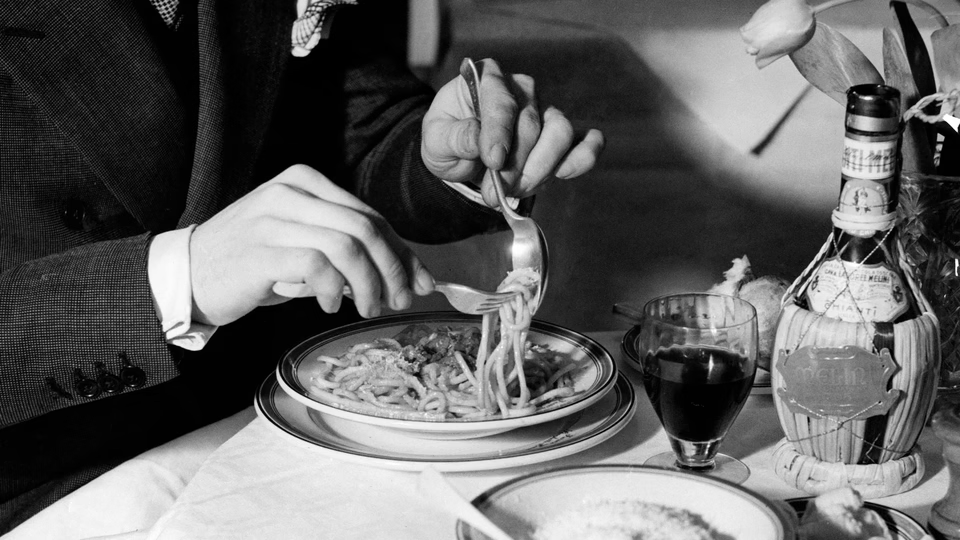
\includegraphics[width=1\textwidth]{original.png} % Adjust the width as needed
  %  \vspace{0.3cm} % Reduced space after the image

    % Left-align everything else
  %  \raggedright % Switch to left alignment

    % Title of the Note
   % {\Huge\bfseries ECON3011 Assignment: Macaronia\par}
   % \vspace{0.8cm} % Reduced space after the title
% Course Name and Number
%{\Large\bfseries Course Name: ECON3011 Economics of Financial Institutions\par}
% Name of Student with IDs
%{\Large\bfseries Khai Jones: 400019518\par}
%{\Large\bfseries Carly Jordan: 400017108\par}
%{\Large\bfseries Nikayla Als: 400018491\par}



% Faculty
%{\Large\bfseries Faculty: Social Sciences\par}

% Date
 %   {\Large Date: \today\par} % Automatically inserts the current date
  %  {\Large\bfseries Group H\par}
   % \vspace{0.8cm} % Reduced space after the faculty
%\end{titlepage}

% PROJECT %
%------------% 
%Title Page 
% % Title Page
\begin{titlepage}
    \centering % Center everything on the title page

    % Title of the document
    \vspace*{2cm} % Add some space at the top
    {\Huge\bfseries The Economic Crisis in the Democratic Republic of Macaronia: A Comprehensive Analysis and Policy Recommendations\par}
    \vspace{1.5cm} % Add some space after the title

    % Subtitle or additional information (optional)
    {\Large\itshape Addressing Systemic Risks and Stabilizing the Financial Sector\par}
    \vspace{2cm} % Add some space after the subtitle

    % Author name (optional)
    {\Large\bfseries Addressed To Governor Lesetja Kganyago }
    \vspace{1cm} % Add some space after the author name
 
    \vspace{2cm} % Add some space after the institution

    % Date (optional)
    {\Large \today\par} % Automatically inserts the current date
    \vfill % Fill the rest of the page with space

    % Optional: Include a logo or image (if needed)
    % \includegraphics[width=0.4\textwidth]{logo.png} % Replace 'logo.png' with your image file

    \vspace{3cm} % Add some space at the bottom
\end{titlepage}

% Introduction 
% \section*{Introduction}



The Democratic Republic of Macaronia is experiencing a \textbf{\textcolor{teal}{severe financial crisis}} caused by global economic shocks and domestic vulnerabilities. Once a flourishing economy with rapid economic expansion, fueled by aggressive credit expansion, a \textbf{\textcolor{teal}{booming real estate sector}}, and high foreign direct investment, Macaronia now faces financial distress. The recent collapse of a \textbf{\textcolor{teal}{major U.S. financial institution}} has created instability in the global credit market, triggering \textbf{\textcolor{teal}{capital flight}}, a drastic decline in Macaronia’s stock market performance, and increased liquidity pressure on the domestic banking sector. As a result, two commercial banks have already failed, and \textbf{\textcolor{teal}{deposit outflows}} are threatening the stability of the financial system.  

In light of these developments, this research note will provide an assessment of the current economic and financial state of Macaronia, with suggestions for possible intervention strategies by the \textbf{\textcolor{teal}{Central Bank}} to stabilize the financial sector while mitigating long-term economic risks. It provides a background on the economy, outlines major financial and macroeconomic variables, and sets forth the \textbf{\textcolor{teal}{policy options}} for the Central Bank. Adjustments to \textbf{\textcolor{teal}{monetary policy}}, management of the exchange rate and reserves, and stability for the financial sector form part of the analysis. Given the \textbf{\textcolor{teal}{urgency of the situation}}, this note presents a clear and data-driven set of recommendations to inform policy decisions.

%Background and Stylised Facts 
%
\section*{Background and Stylised Facts}



\subsection*{Macaronia's Economic Landscape}


In the past decade, the economic development of the \textcolor{teal}{Democratic Republic of Macaronia}, a 
small open economy with a \textcolor{teal}{floating exchange rate} and a population of 4.6 million, was
primarily \textcolor{teal}{FDI-led} and accelerated due to aggressive credit expansion. However, as global 
financial markets fall into turmoil, the country's financial system could face significant risks due to 
domestic vulnerabilities. 

The IMF projects a contraction in \textcolor{teal}{global economic growth} to 2.5\% in 2023 and
3\% in 2024, which is predicted to hit small economies like Macaronia extremely hard.
This  may reduce external investment, increase risks within the financial system, and
 contribute to instability.

Rising \textcolor{teal}{inflation}, heightened tensions in the financial sector, and declining 
\textcolor{teal}{investor confidence} further compound the downside risks to Macaronia’s economy.
A reduction in \textcolor{teal}{foreign capital inflows} could constrain credit conditions and hinder growth. 
If financial stress deepens, reliance on \textcolor{teal}{foreign financing} may expose the country to additional
vulnerabilities, complicating efforts by policymakers to stabilize the economy.

\subsection*{Macaronia's Economic Performance}

% Insert "Real GDP Growth" graph here 
% Insert "Inflation Trends" graph here

\begin{figure}[h]
    \centering
    \begin{subfigure}{0.48\textwidth}
        \centering
        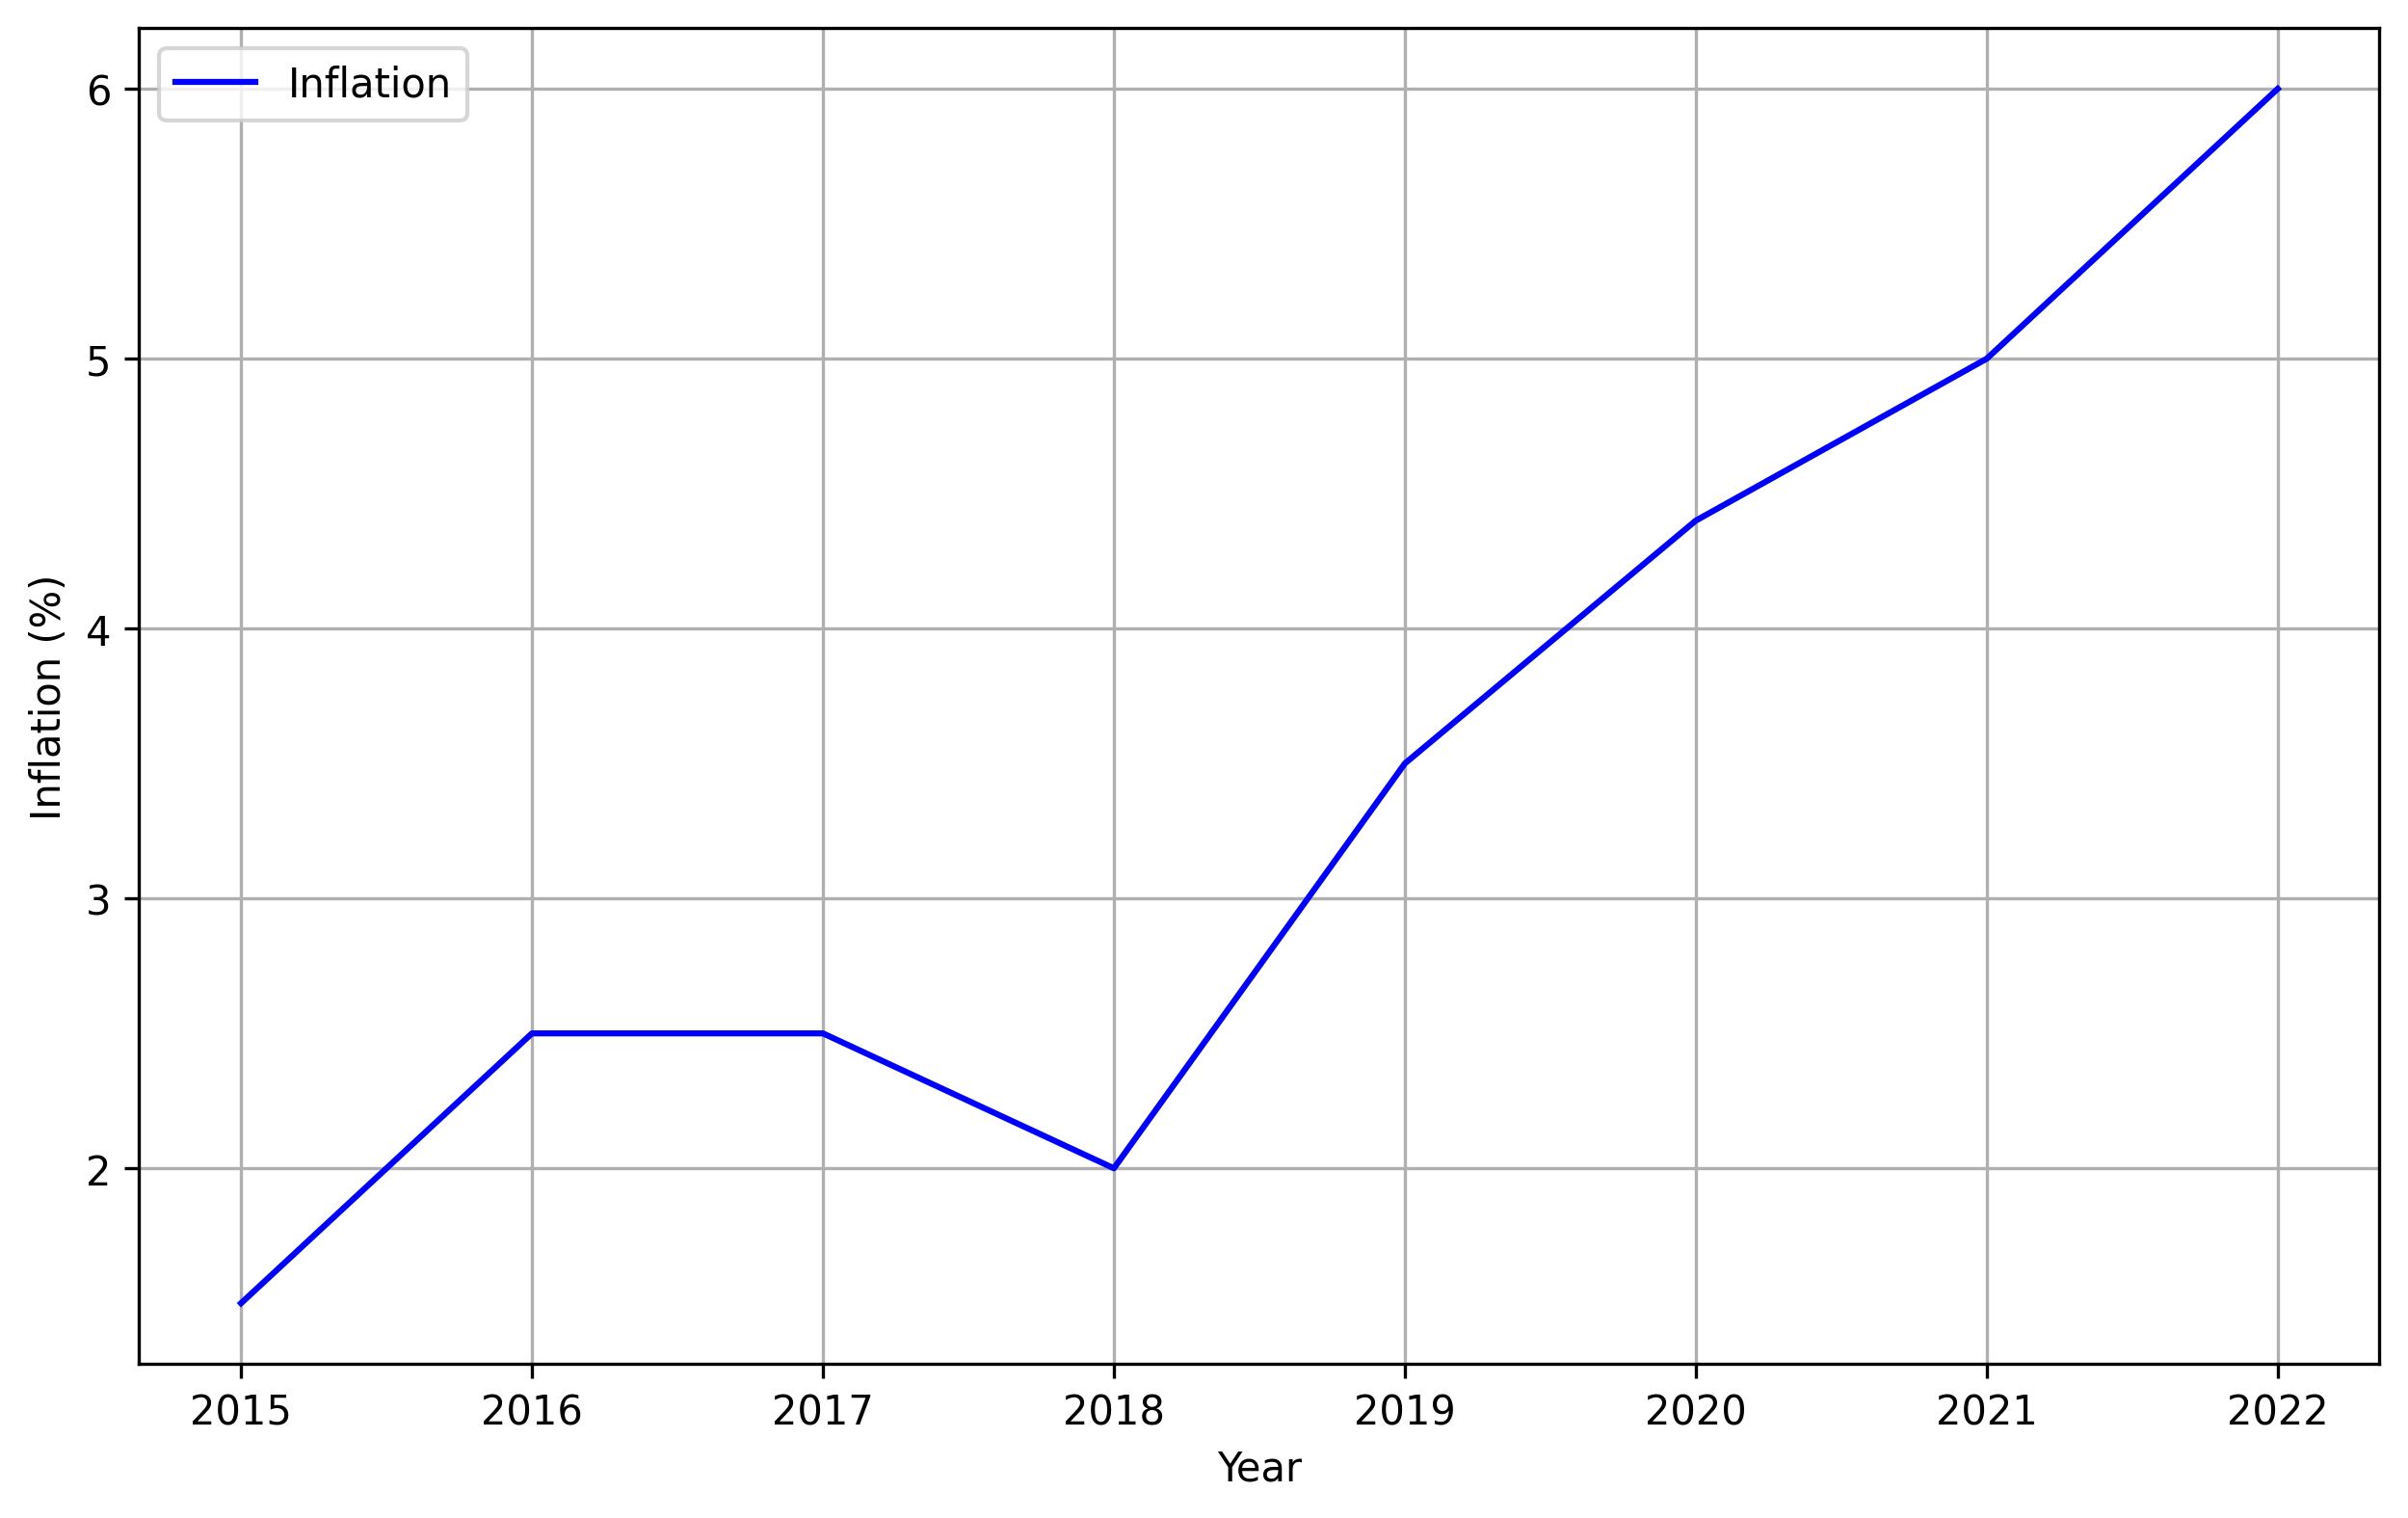
\includegraphics[width=\textwidth]{inflation.png}
        \caption{\small Inflation Rate}
        \label{fig:inflation}
    \end{subfigure}
    \hfill
    \begin{subfigure}{0.48\textwidth}
        \centering
        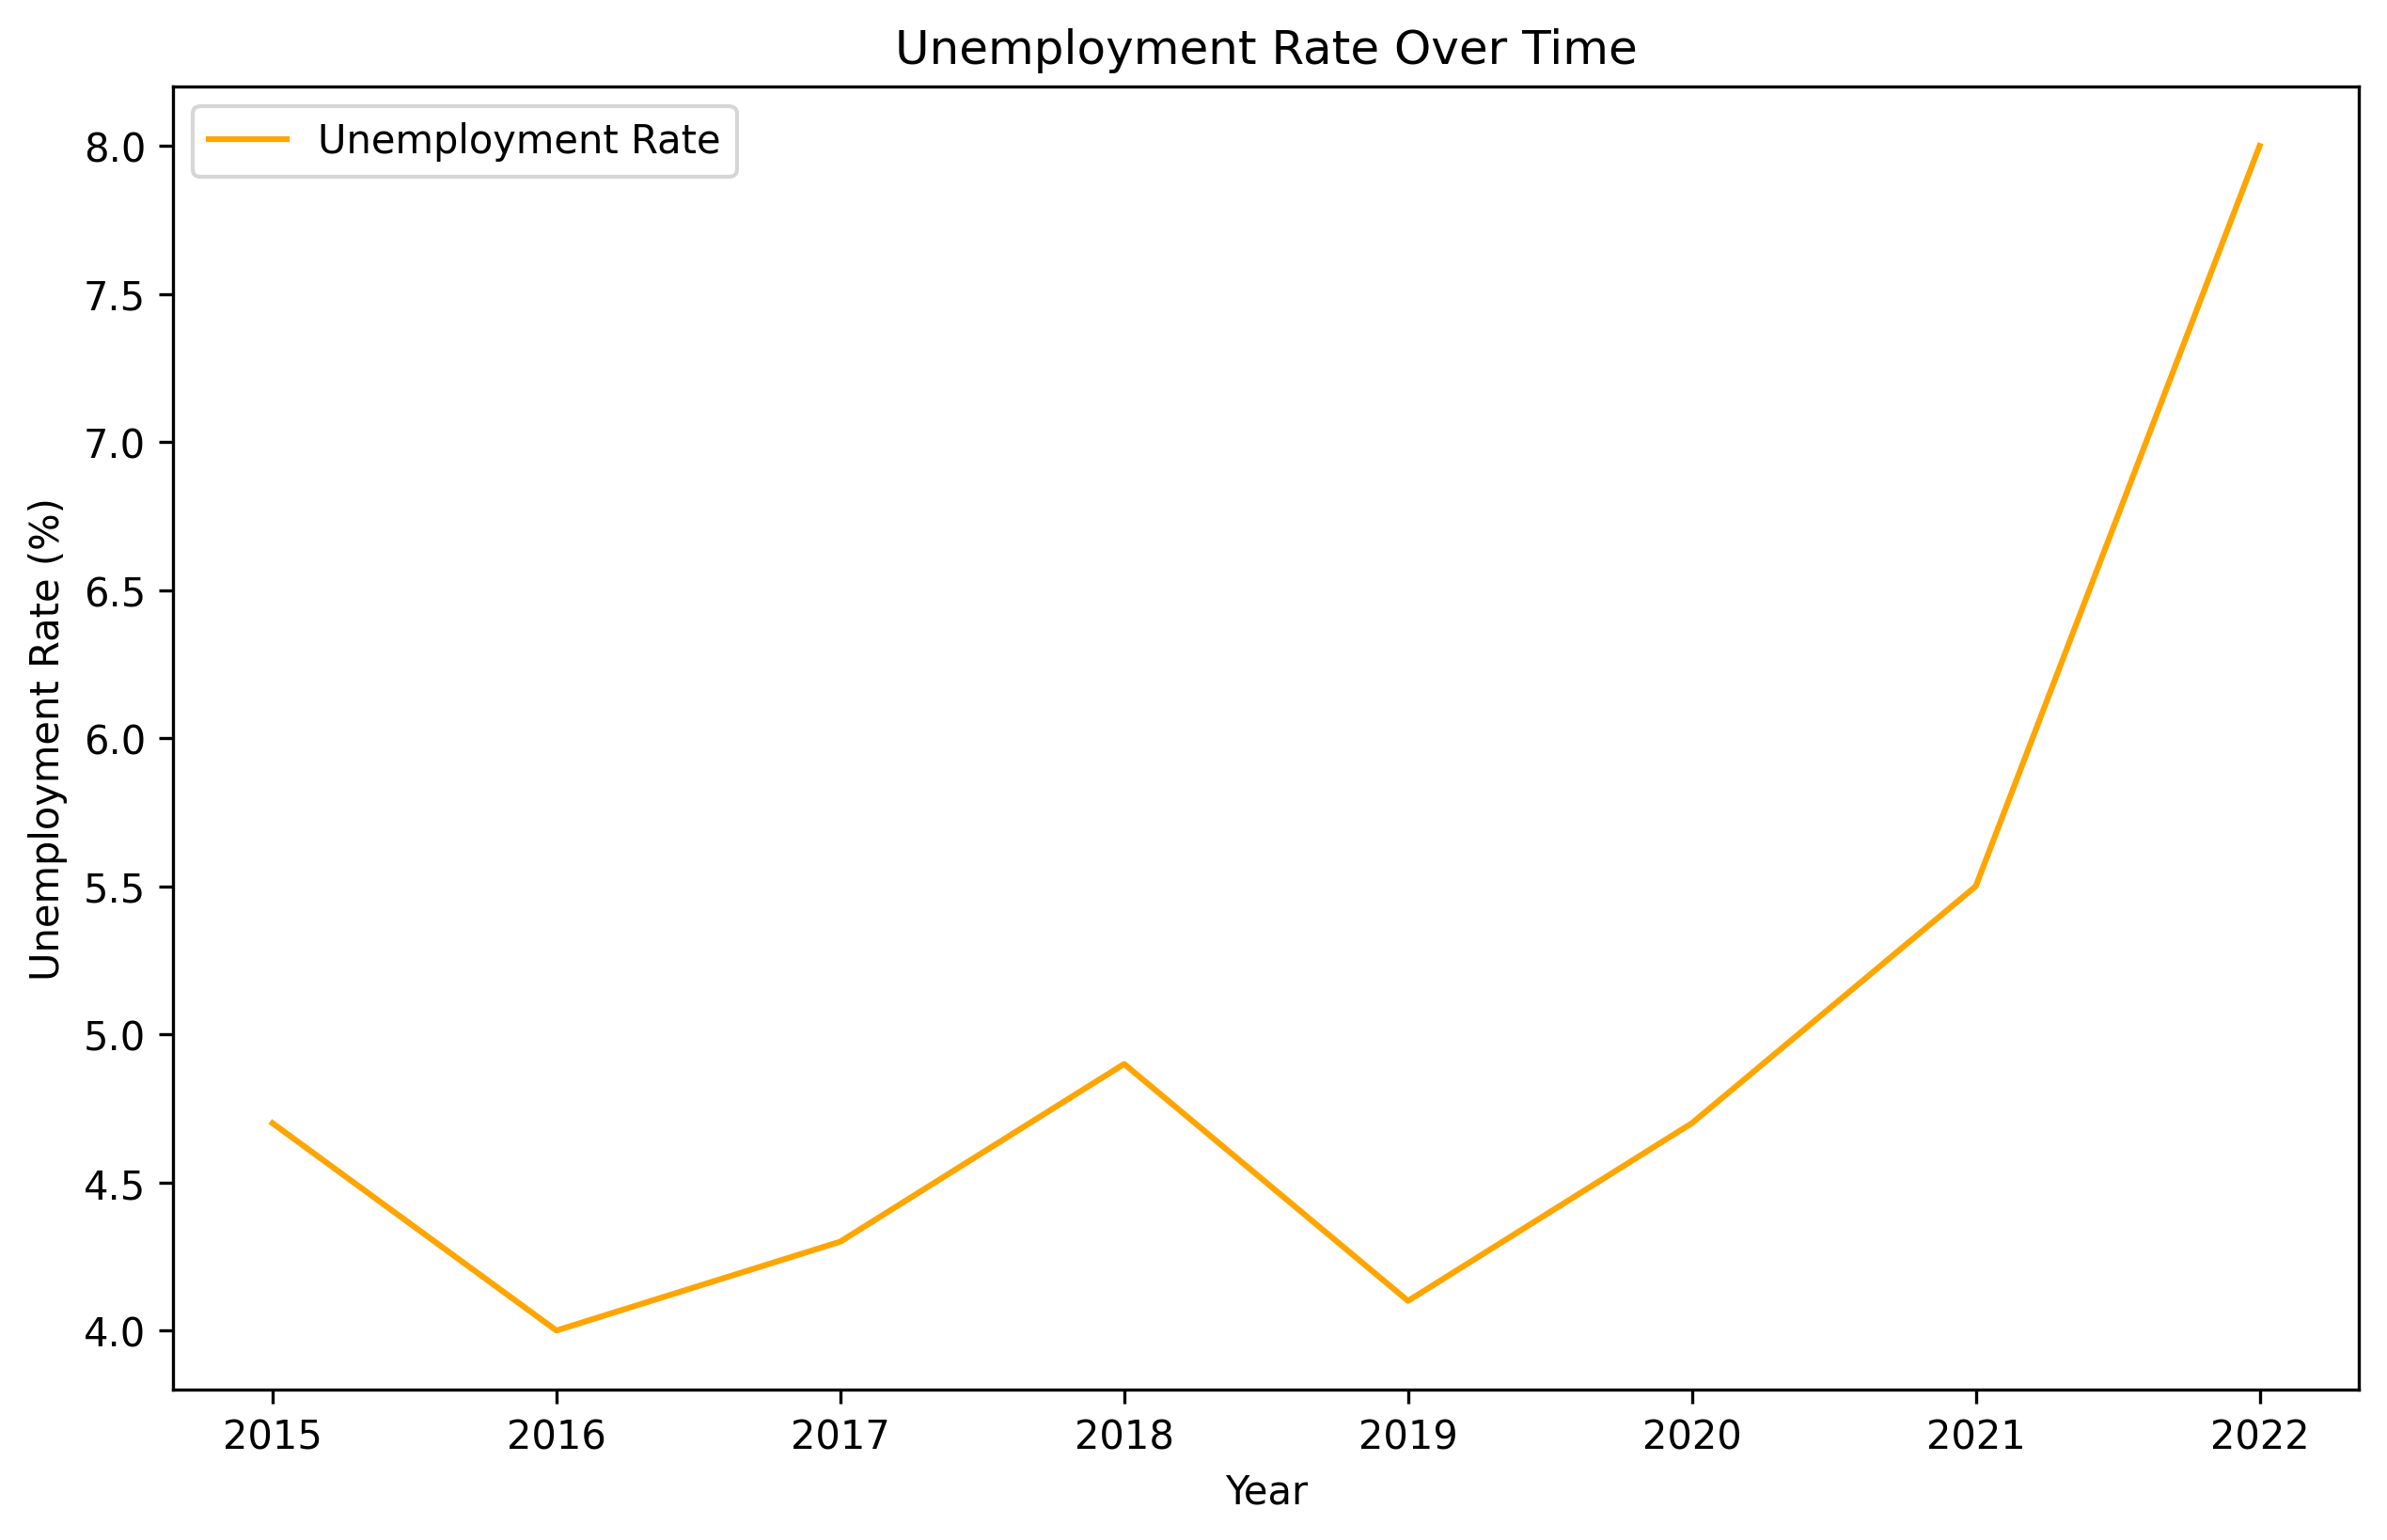
\includegraphics[width=\textwidth]{unemployment.png}
        \caption{\small Unemployment Rate}
        \label{fig:unemployment}
    \end{subfigure}
    \caption{Inflation and Unemployment Trends}  % Main caption for the whole figure
    \label{fig:main_figure}  % Main label for reference
\end{figure}


Macaronia's economy expanded at an average rate of 
\textcolor{teal}{\textbf{4.8\%}}, supported by a booming real estate market. However,
in 2022, the economy contracted by \textcolor{teal}{\textbf{3\%}}, marking the first downturn in nearly a 
decade. The slowdown was mainly driven by the sharp depreciation of REIT values, declining investor confidence,
and tighter global financial conditions.

Figure 1(a) illustrates that inflation rose significantly from \textcolor{teal}{\textbf{1.5\%}}
in 2015 to \textcolor{teal}{\textbf{6\%}} in 2022, fueled by both external price pressures and domestic 
structural vulnerabilities. This surge has been aggravated by the depreciation of the exchange rate and
higher commodity prices, reducing household purchasing power. At the same time, Figure 1(b) demonstrates
that unemployment increased to \textcolor{teal}{\textbf{8\%}} in 2022 from \textcolor{teal}{\textbf{4.7\%}} 
in 2015, as economic activity slowed and businesses reduced hiring. The simultaneous rise 
in \textcolor{teal}{\textbf{inflation}} and \textcolor{teal}{\textbf{unemployment}}, as depicted in
Figures 1(a) and 1(b), suggests that Macaronia is experiencing \textcolor{teal}{\textbf{stagflation}}, 
a challenging economic condition characterized by slow growth, high inflation, and rising unemployment.


\subsection*{Financial Sector Risks and Credit Growth}



Macaronia’s financial system, including commercial banks, credit unions, and insurance companies, 
has expanded greatly in recent years. At the same time, concerns have grown over increasing 
\textcolor{teal}{systemic risks}, especially with excessive exposures to volatile assets like 
\textcolor{teal}{REITs}.  

The commercial banking sector holds assets worth \textcolor{teal}{MCR\$32.0 billion} 
(\textcolor{teal}{20\%} of GDP), with \textcolor{teal}{15\%} of total assets tied up in REITs. 
Credit unions, while smaller, have \textcolor{teal}{MCR\$15.0 billion} in assets, with 
\textcolor{teal}{25\%} of those in REITs.  

The banking sector’s \textcolor{teal}{liquidity position} has weakened, as 
deposit withdrawals have increased in response to concerns about financial stability.
Liquidity ratios dropped from \textcolor{teal}{75\%} in 2020 to \textcolor{teal}{65\%} 
in 2022 for commercial banks, and from \textcolor{teal}{78.8\%} to \textcolor{teal}{68.3\%}
for credit unions. However, \textcolor{teal}{capital adequacy} remains above regulatory benchmarks,
with \textcolor{teal}{12\%} for banks and \textcolor{teal}{10\%} for credit unions.  

These trends align with Diamond and Dybvig’s (1983) model of \textcolor{teal}{bank runs},
which highlights how liquidity mismatches and depositor panic can trigger financial crises. 
The failure of \textcolor{teal}{two} commercial banks in Macaronia due to poor capitalization and
deteriorating asset values underscores these risks.  

\subsection*{Public Sector Debt and Fiscal Position}

\begin{figure}[h]
    \centering
    \begin{subfigure}{0.48\textwidth}
        \centering
        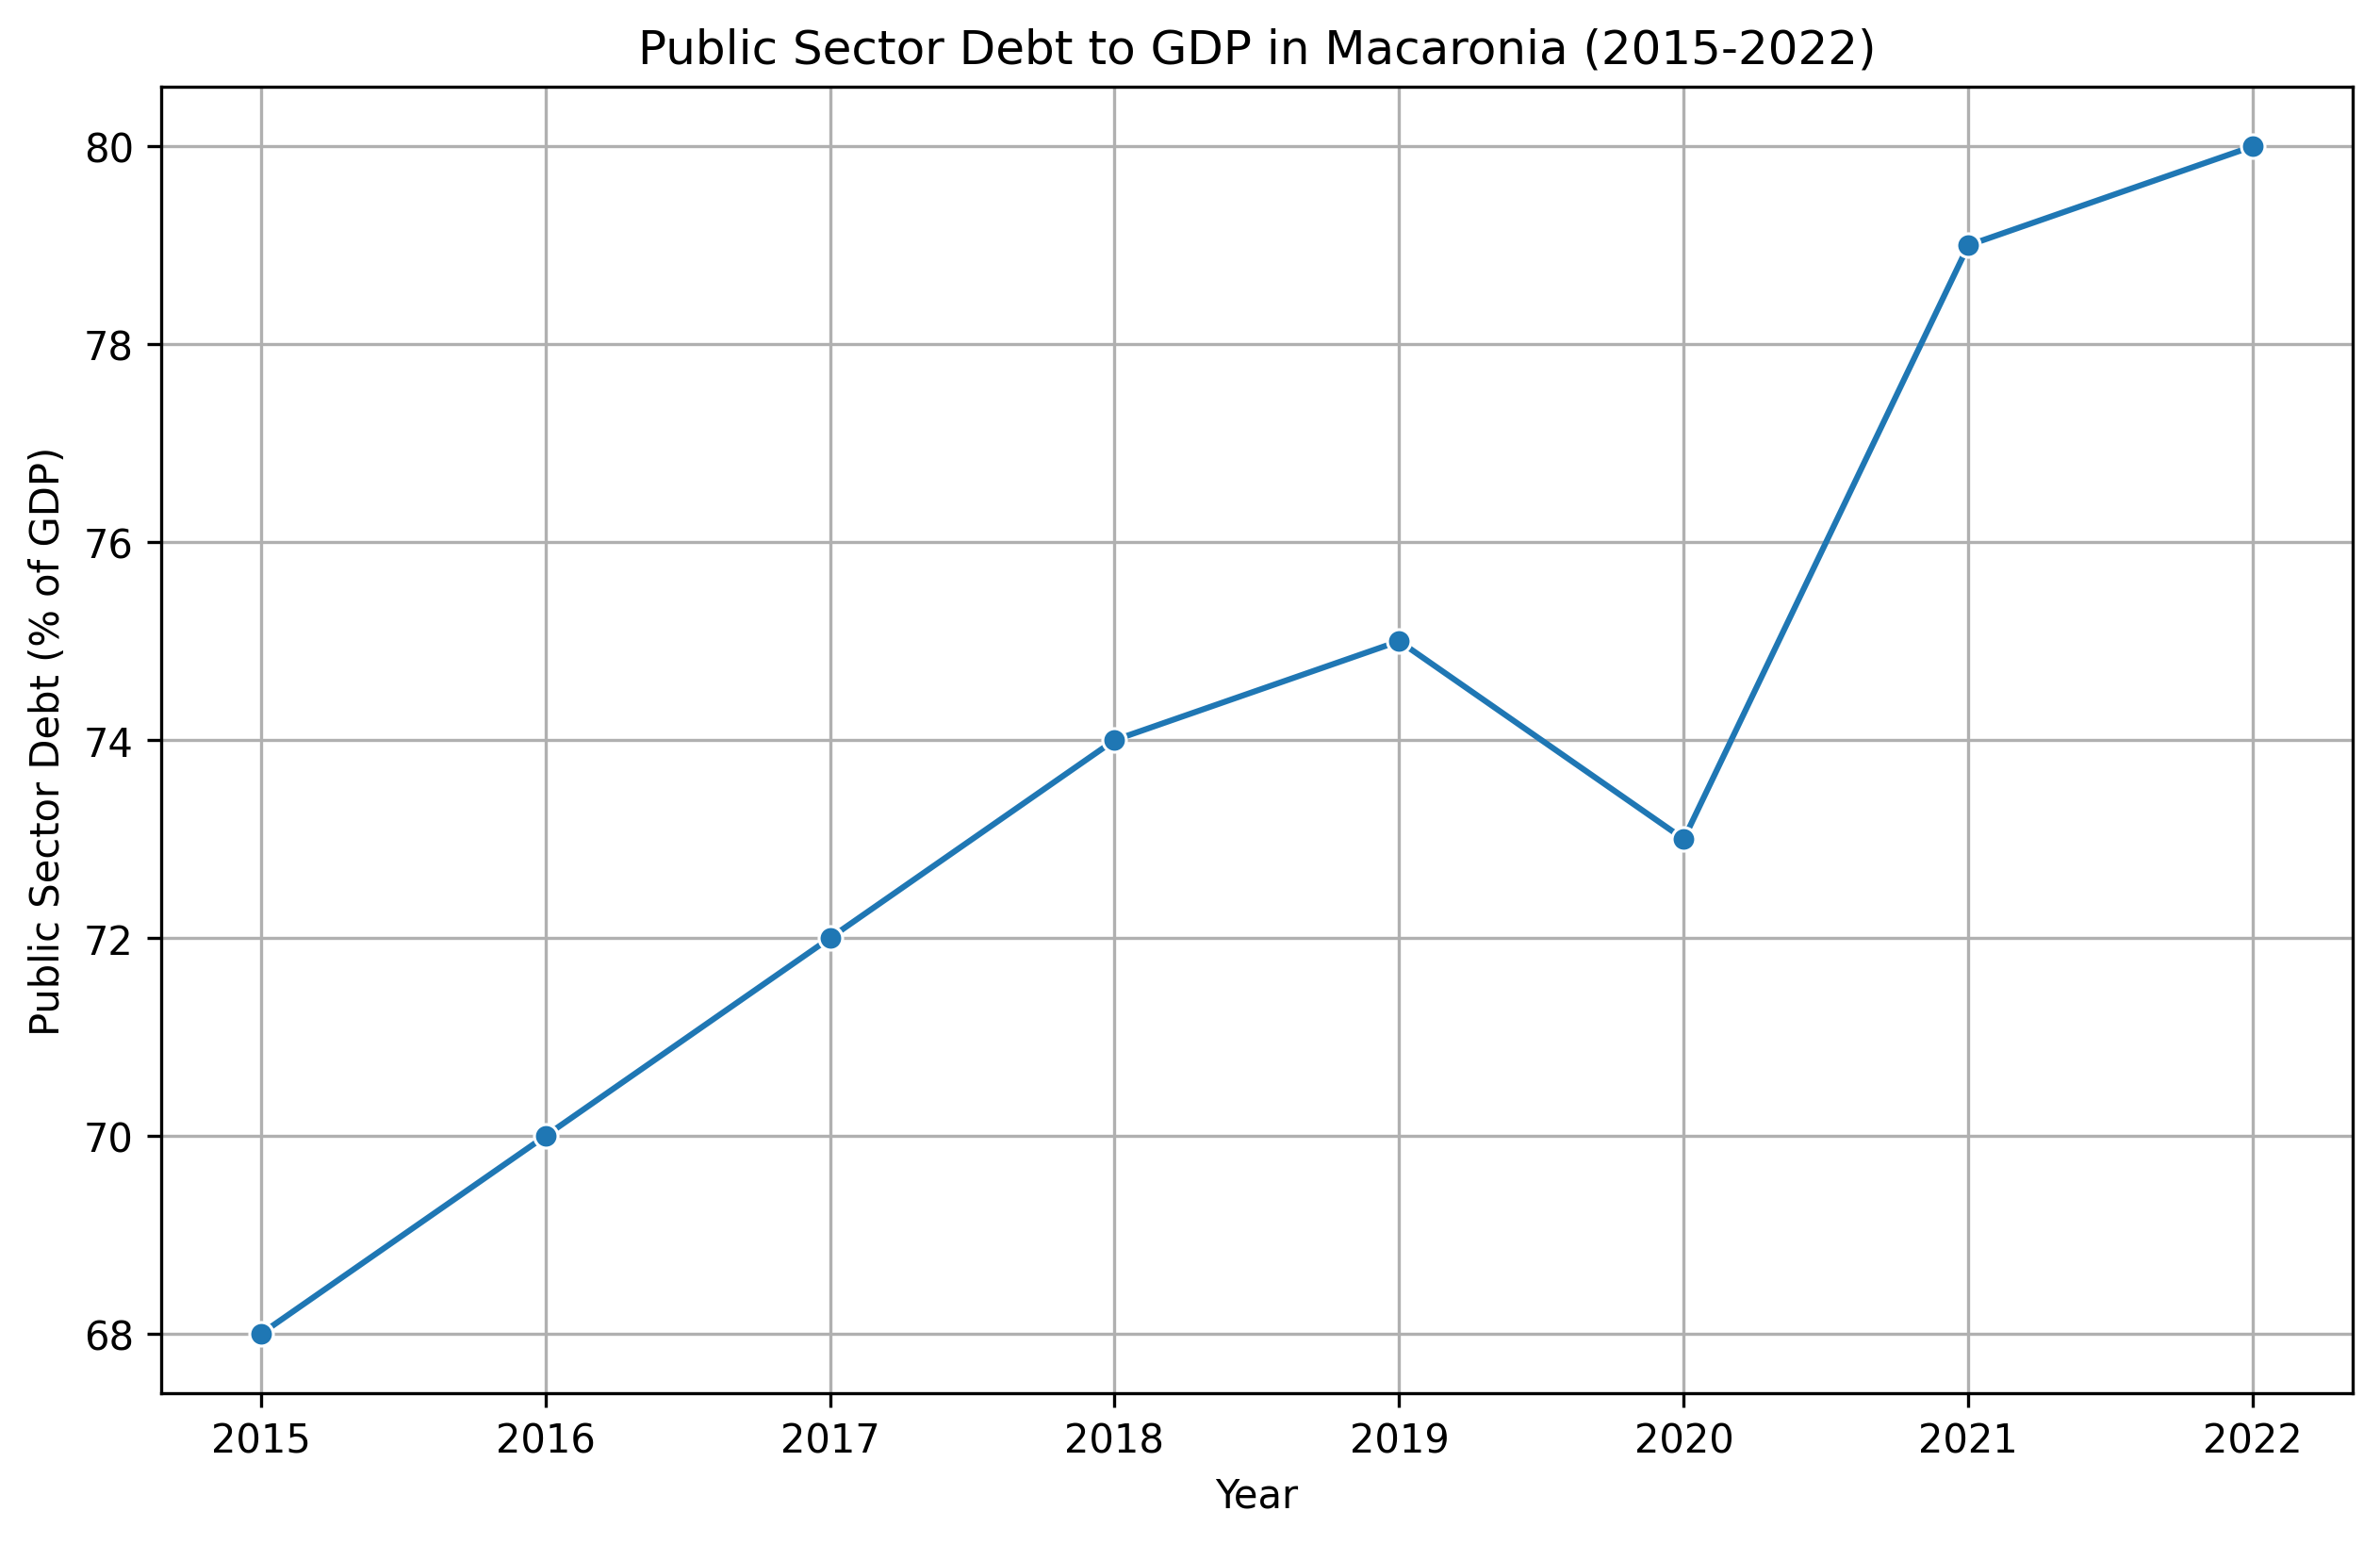
\includegraphics[width=\textwidth]{debt_to_gdp.png}
        \caption{\small Public Sector Debt to GDP in Macaronia}
        \label{fig:debt_to_gdp}
    \end{subfigure}
    \hfill
    \begin{subfigure}{0.48\textwidth}
        \centering
        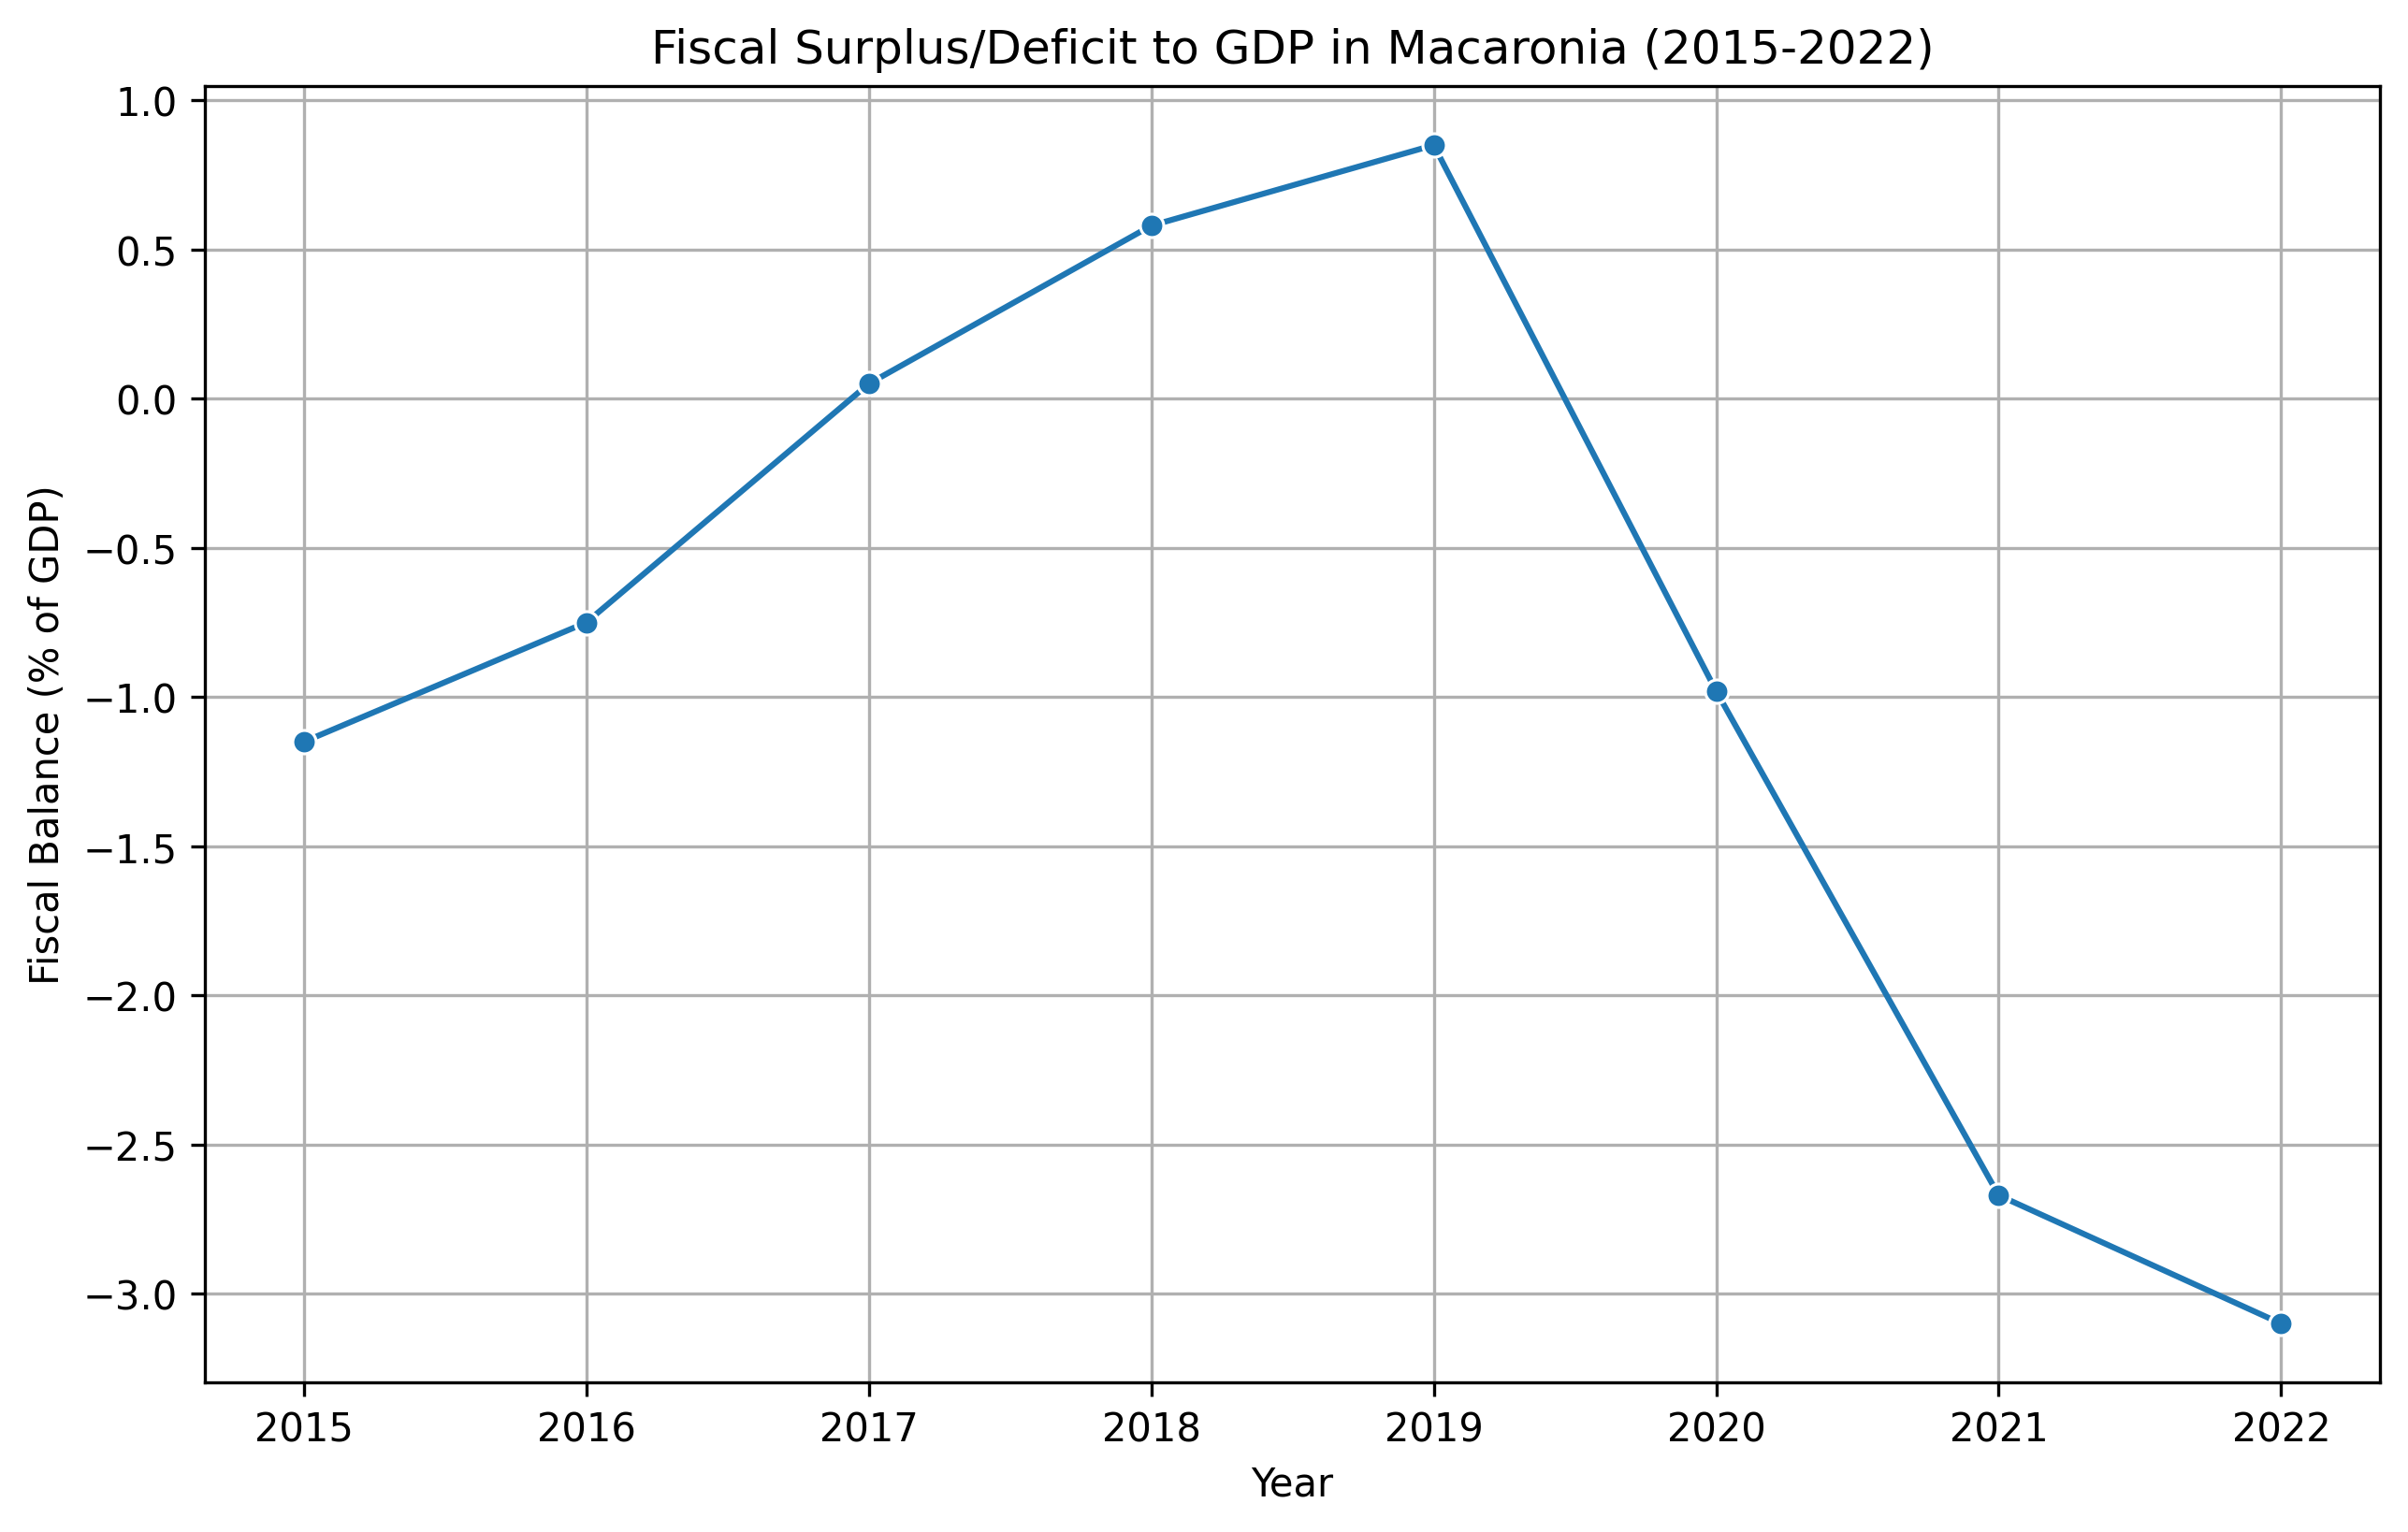
\includegraphics[width=\textwidth]{fiscal_to_gdp.png}
        \caption{\small Fiscal Surplus/Deficit to GDP in Macaronia}
        \label{fig:fiscal_to_gdp}
    \end{subfigure}
    \caption{Macaronia’s Public Debt and Fiscal Position (2015-2022)}  % Main figure caption
    \label{fig:public_debt_fiscal}
\end{figure}


As depicted in Figure 2(a), Macaronia's public sector debt has steadily increased, reaching
\textcolor{teal}{\textbf{80\% of GDP}} in 2022 from \textcolor{teal}{\textbf{68\% of GDP}} 
in 2015, reflecting a concerning trend. This trajectory indicates a growing reliance on borrowing
to finance government expenditures. Concurrently, Figure 2(b) illustrates a significant deterioration
in the fiscal position, with \textcolor{teal}{\textbf{fiscal deficits}} widening to 
\textcolor{teal}{\textbf{-3.1\% of GDP}} in 2022. This widening deficit suggests that 
government spending has outpaced revenues, contributing to the rising debt burden. 
The combination of high debt levels and persistent deficits raises serious concerns 
about the sustainability of Macaronia's fiscal position, particularly in light of tightening 
\textcolor{teal}{\textbf{global financial conditions}}.

%(Insert "Credit Extended by Banks and Credit Unions" graph here)
%(Insert "Liquidity Ratios – Banks and Credit Unions" graph here)
%(Insert "Capital Adequacy Ratios – Banks and Credit Unions" graph here)

\subsection*{Implications for Economic Theory}

\begin{enumerate}
    \item \colorbold{teal}{Moral Hazard in Financial Regulation}: The moral hazard theory states that financial
                         institutions, particularly banks and credit unions in Macaronia, have taken excessive
                         risks of overexposure to volatile REITs. They operated under the assumption that the
                         central bank would intervene in times of crisis \textcolor{orange}{\cite{holmstrom1997}}. This said
                         behaviour increases systemic risk in the economy. \textcolor{orange}{\cite{allen2015}}.

    \item \colorbold{teal}{Ricardian Equivalence and Public Debt}: The Ricardian Equivalence Theory suggests that rising 
                          public debt may lead to decreased private consumption as people foresee future tax increases.
                          In Macaronia, rising public debt could effectively shrink consumer confidence and as a result,
                          dampen economic recovery.

    \item \colorbold{teal}{Exchange Rate and Reserve Management}: Rapid depleting reserves pose a grave concern for Macaronia’s
                           central bank. According to Mundell’s (1961) theory, a floating exchange rate can repair external 
                           shocks, however, a large depletion of the reserves may force the central bank to intervene to ensure
                           the stability of its currency. \textcolor{orange}{\cite{mundell1961}}
\end{enumerate}

\subsection*{Global Financial Outlook}

% (Insert the "Global Economic Growth" graph here)
\begin{figure}[h]
     \centering
     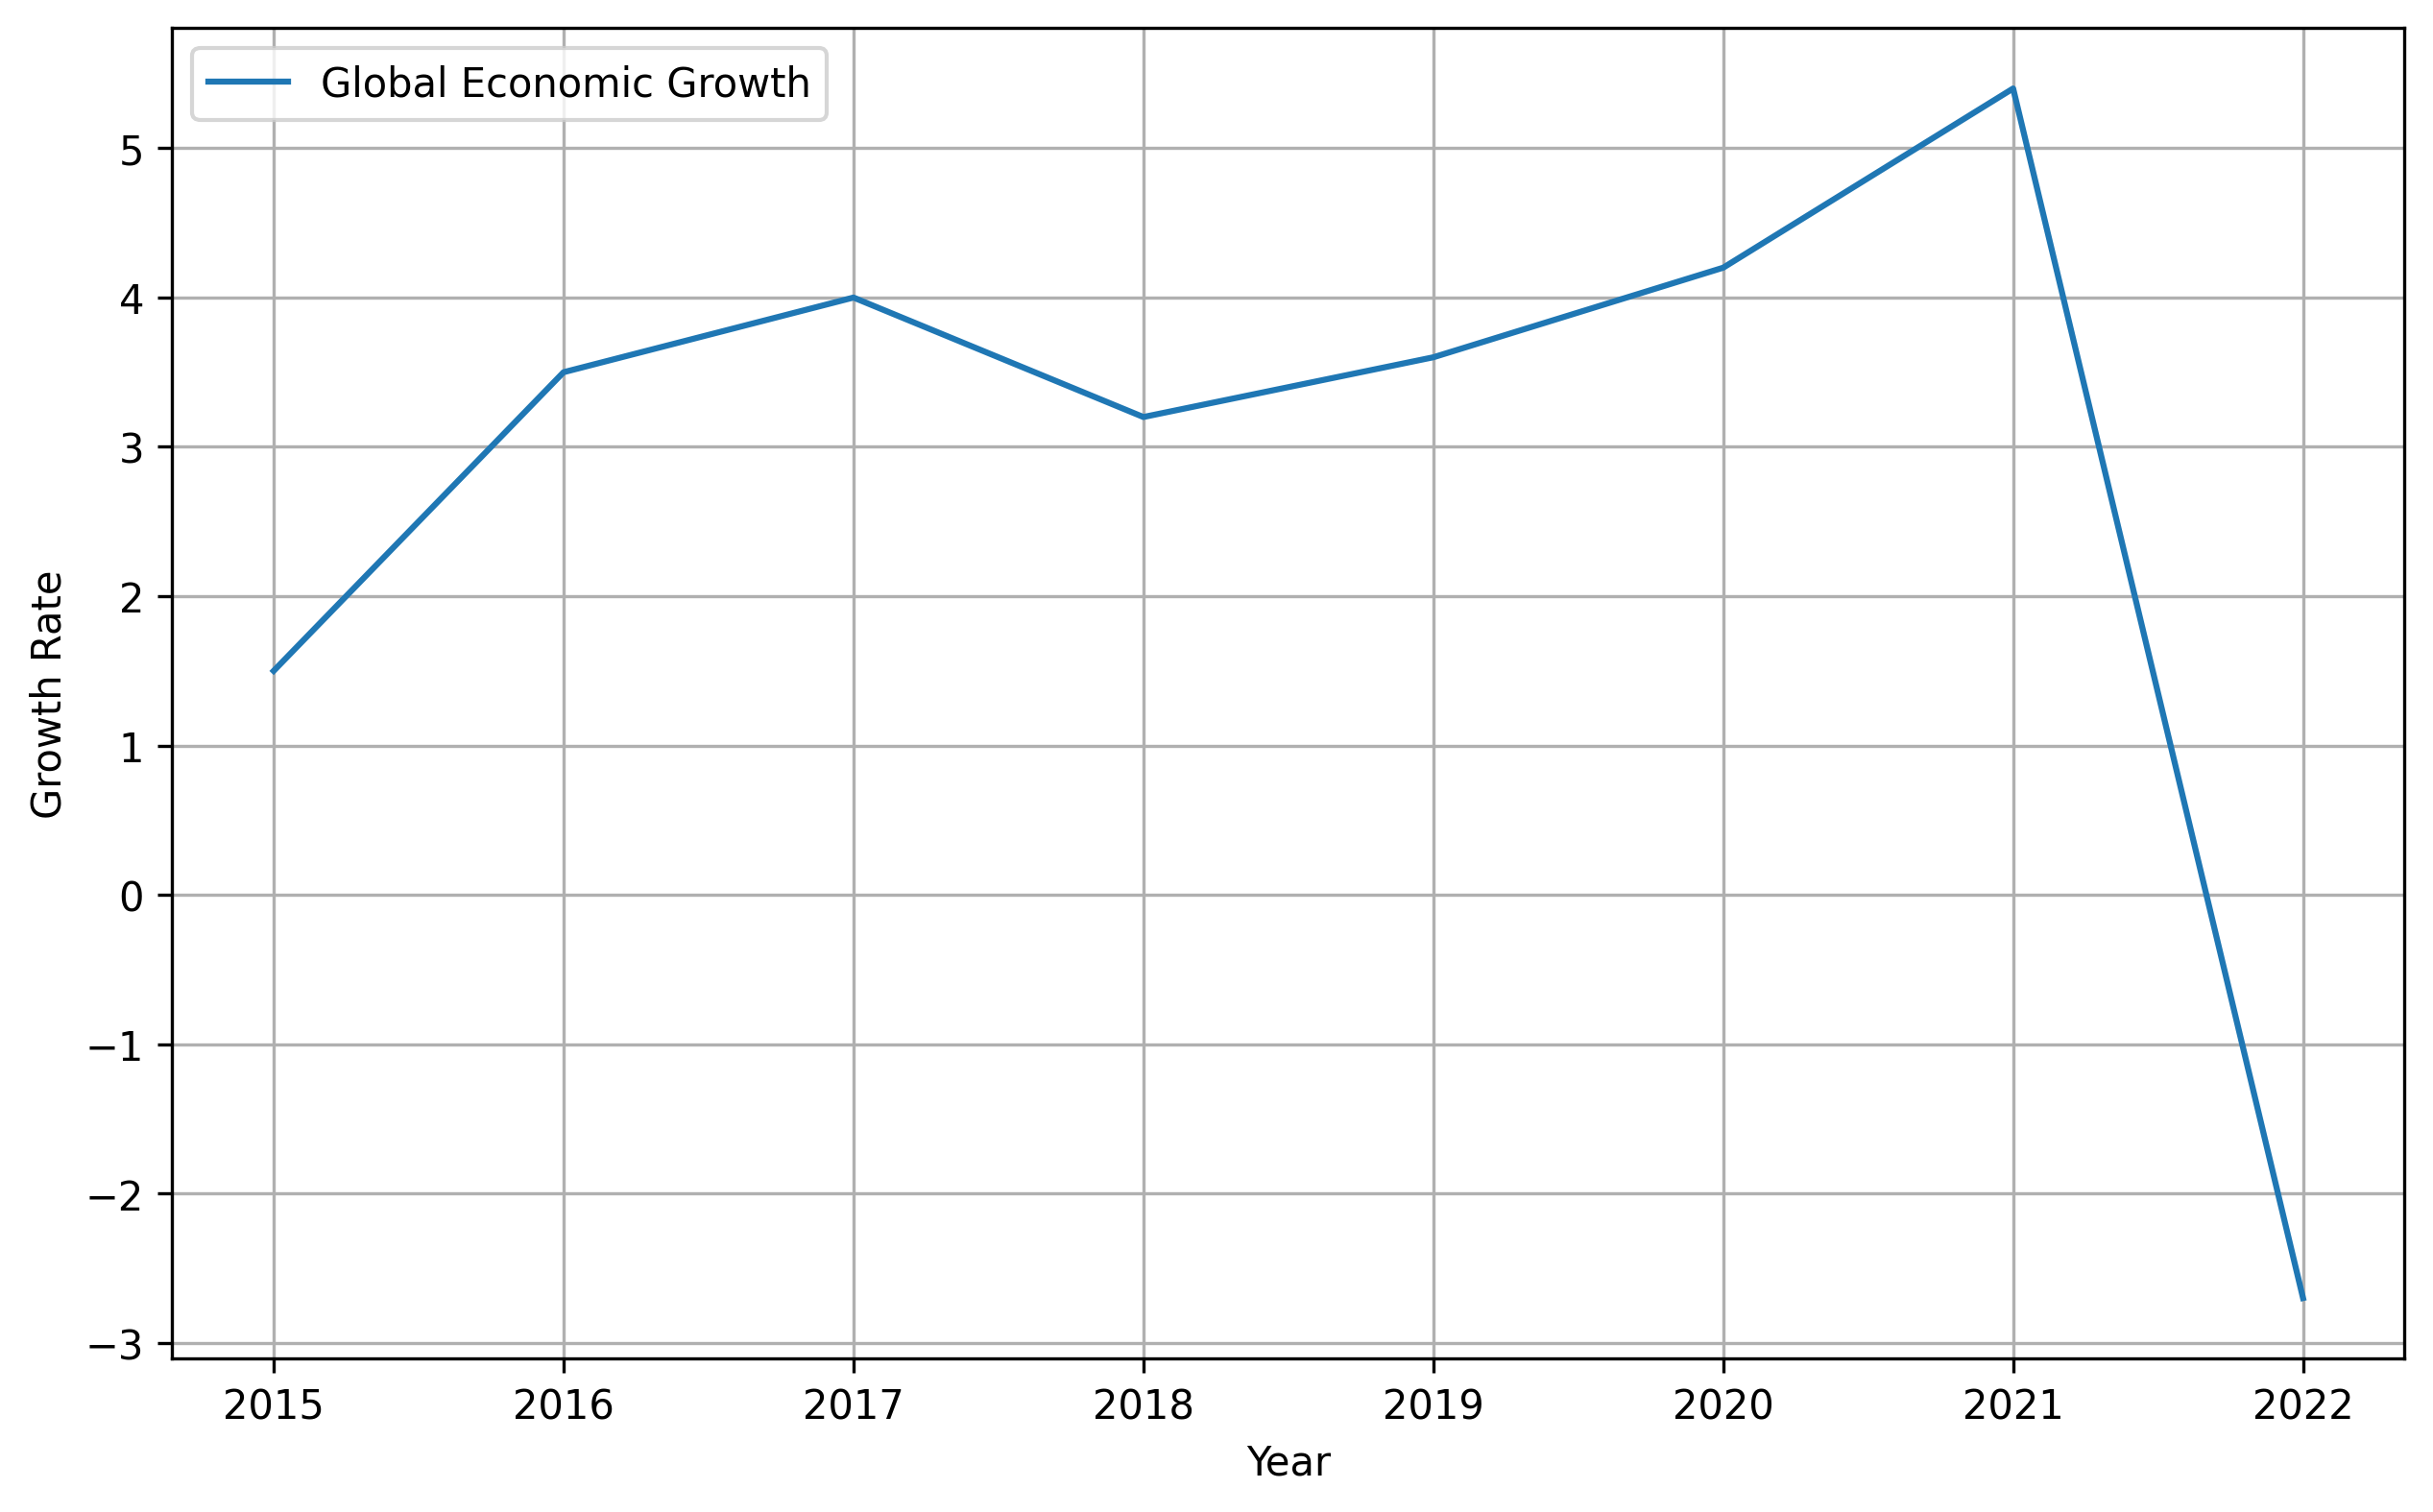
\includegraphics[width=0.6\textwidth]{growth2.png}
     \caption{Global Economic Growth}
     \label{fig:graph_1}
\end{figure}

As depicted in Figure 3, the global economy has experienced significant volatility, with severe shocks 
affecting financial stability. One such shock was due to the collapse of a major U.S. financial institution,
which led to disruptions in global credit markets and increased uncertainty.

As previously mentioned, the IMF estimates a contraction in global economic activity in 2023 by \textcolor{teal}{\textbf{2.5\%}}
and in 2024 by \textcolor{teal}{\textbf{3\%}}. These conditions raise concerns for small, open economies like
Macaronia, which are heavily bound to international financial markets. The ongoing weakening of investor
confidence continues to deplete Macaronia's international reserves due to capital flight, further straining
Macaronia's financial stability.



% Analysis of the Issue
%\onecolumn
\section*{Anaylsis of the Issue}

\begin{figure}[H]
     \centering
     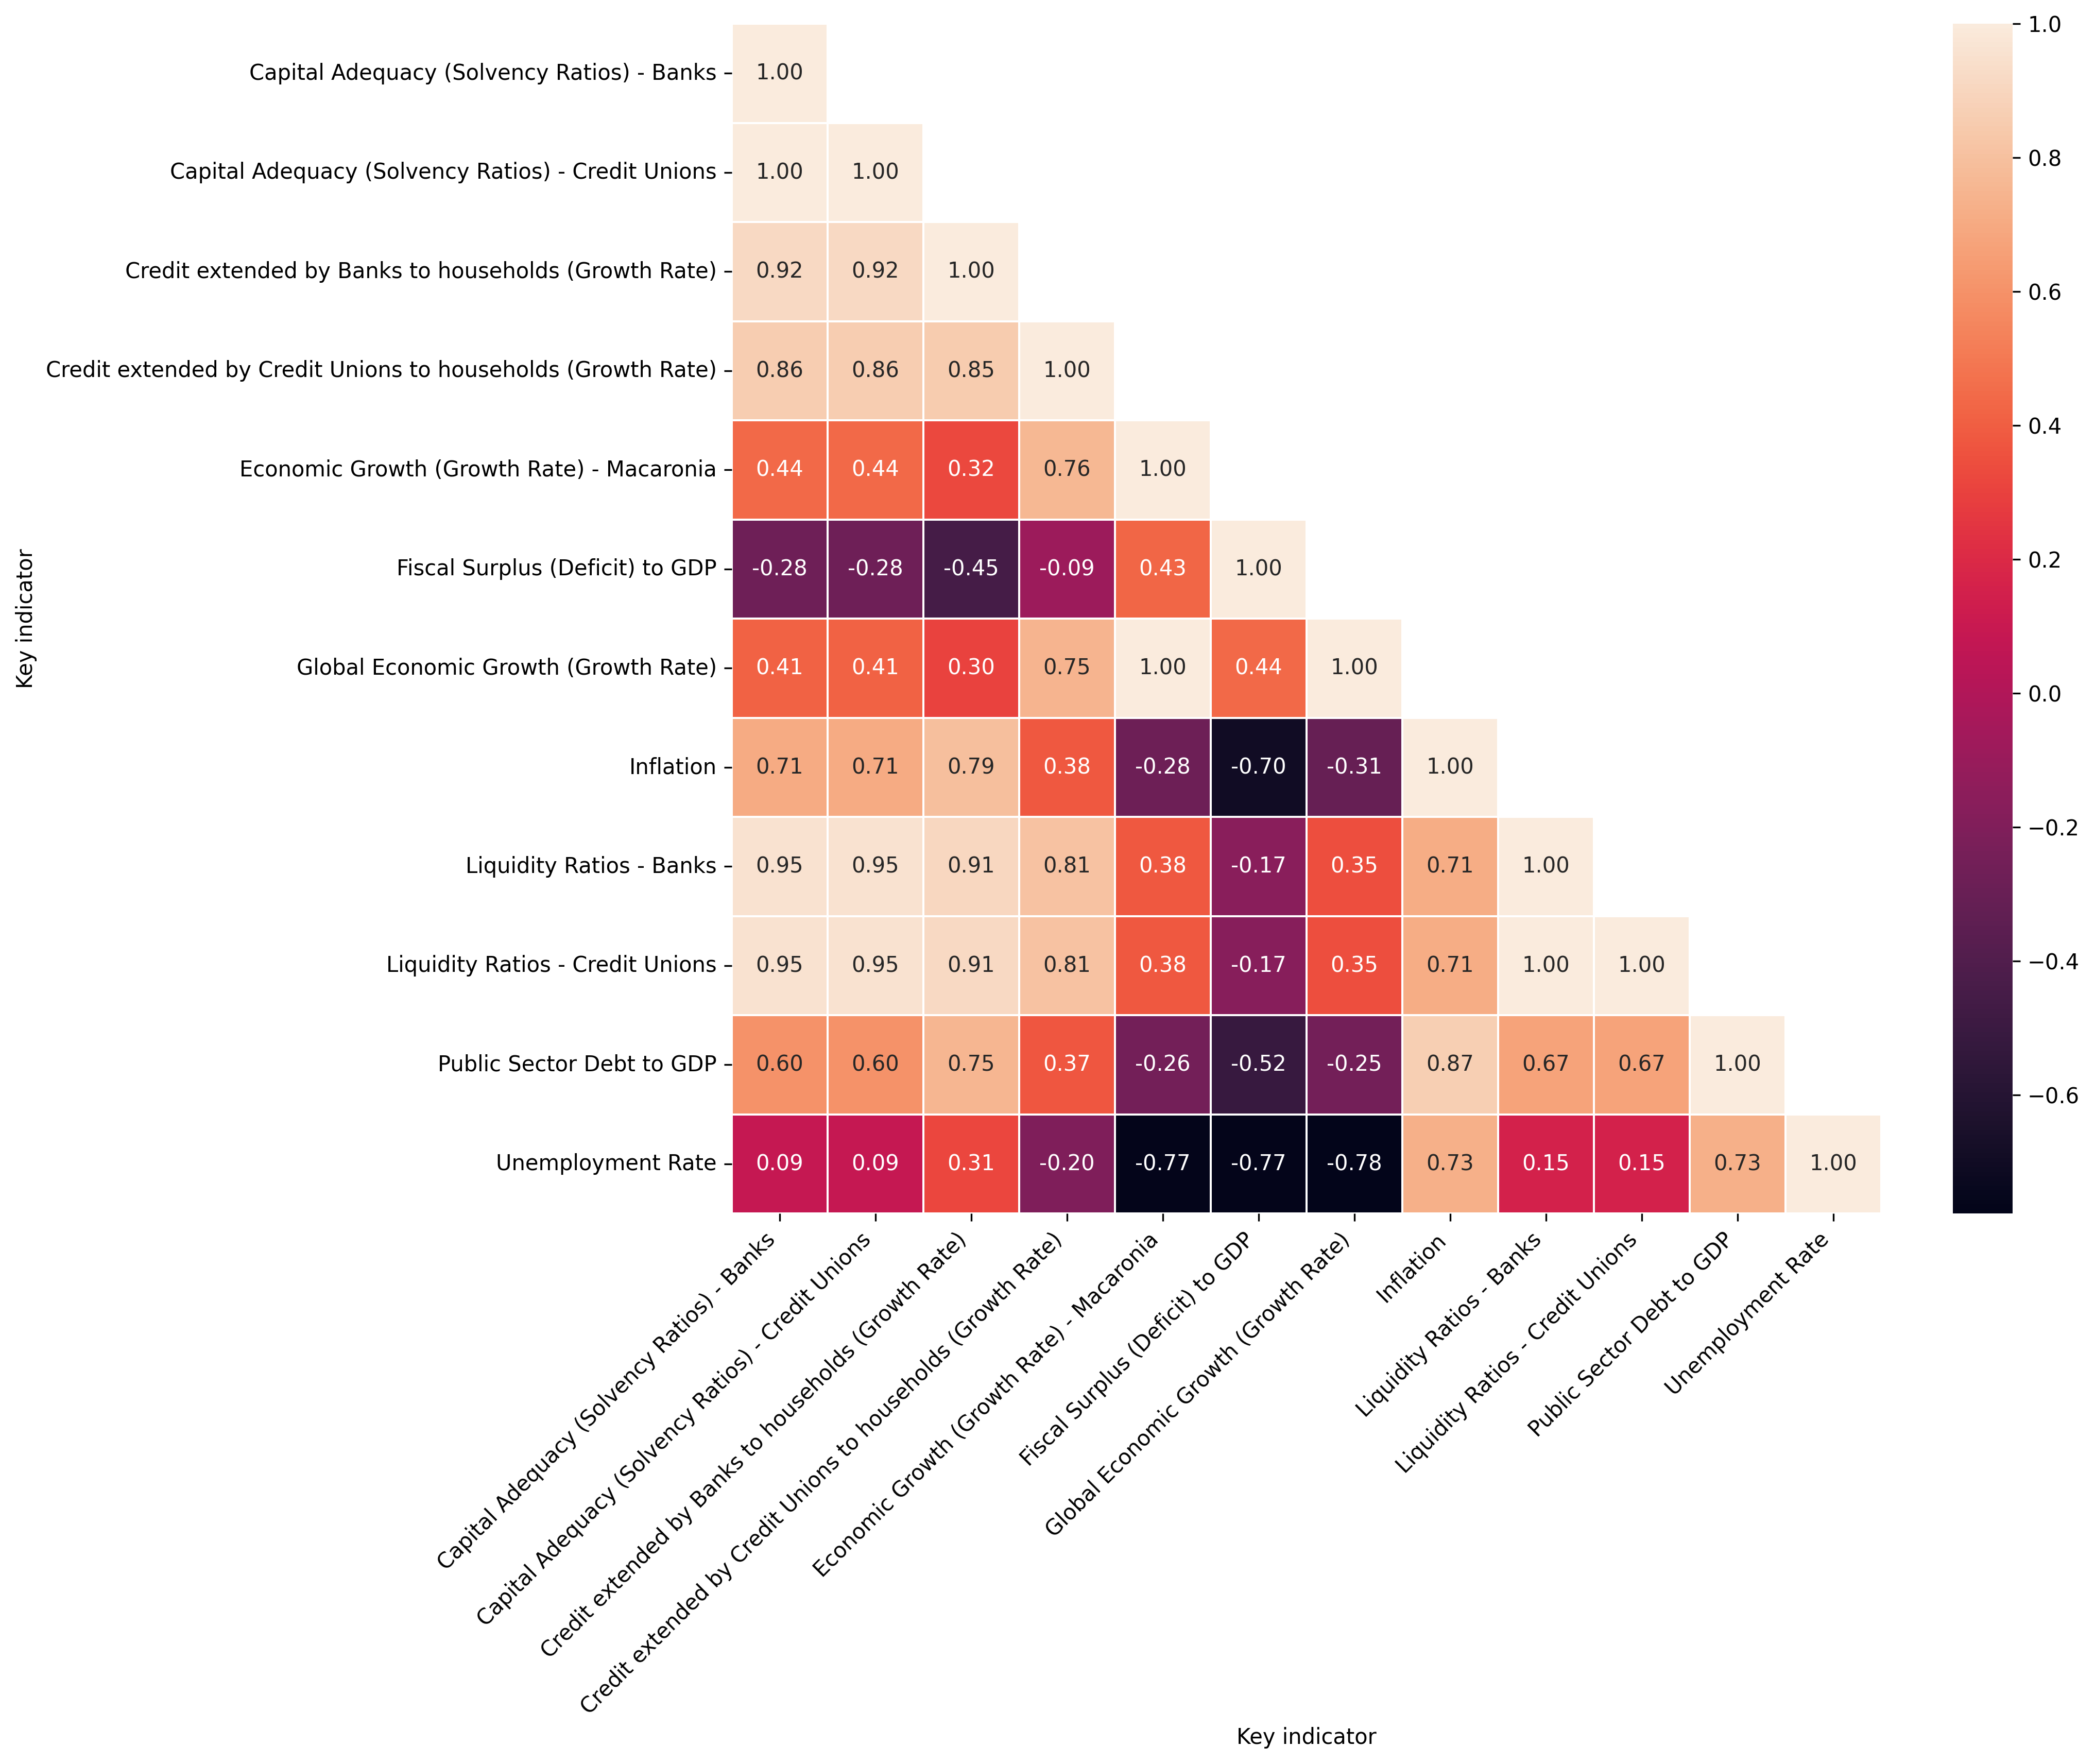
\includegraphics[width=0.86\textwidth]{correlation_matrix.png} % Include the image
     \caption{Correlation Matrix Heatmap}
     \label{fig:correlation_matrix}
\end{figure}


Macaronia’s economic crisis was driven by an aggressive push for growth, but the foundations supporting that growth were far from stable. 
This section begins by assessing the true financial health of banks and credit unions, adjusting their liquidity and capital adequacy ratios to account for credit expansion and risk exposure.
It then examines how heavy investments in REITs heightened financial vulnerabilities, making institutions more susceptible to market shocks. Finally, it explores the key events that triggered the crisis, 
the role of external financial pressures, and the lasting consequences on Macaronia’s economy.



% \newpage
\section{INTERNAL ISSUES}




\begin{figure}[h]
     \centering
     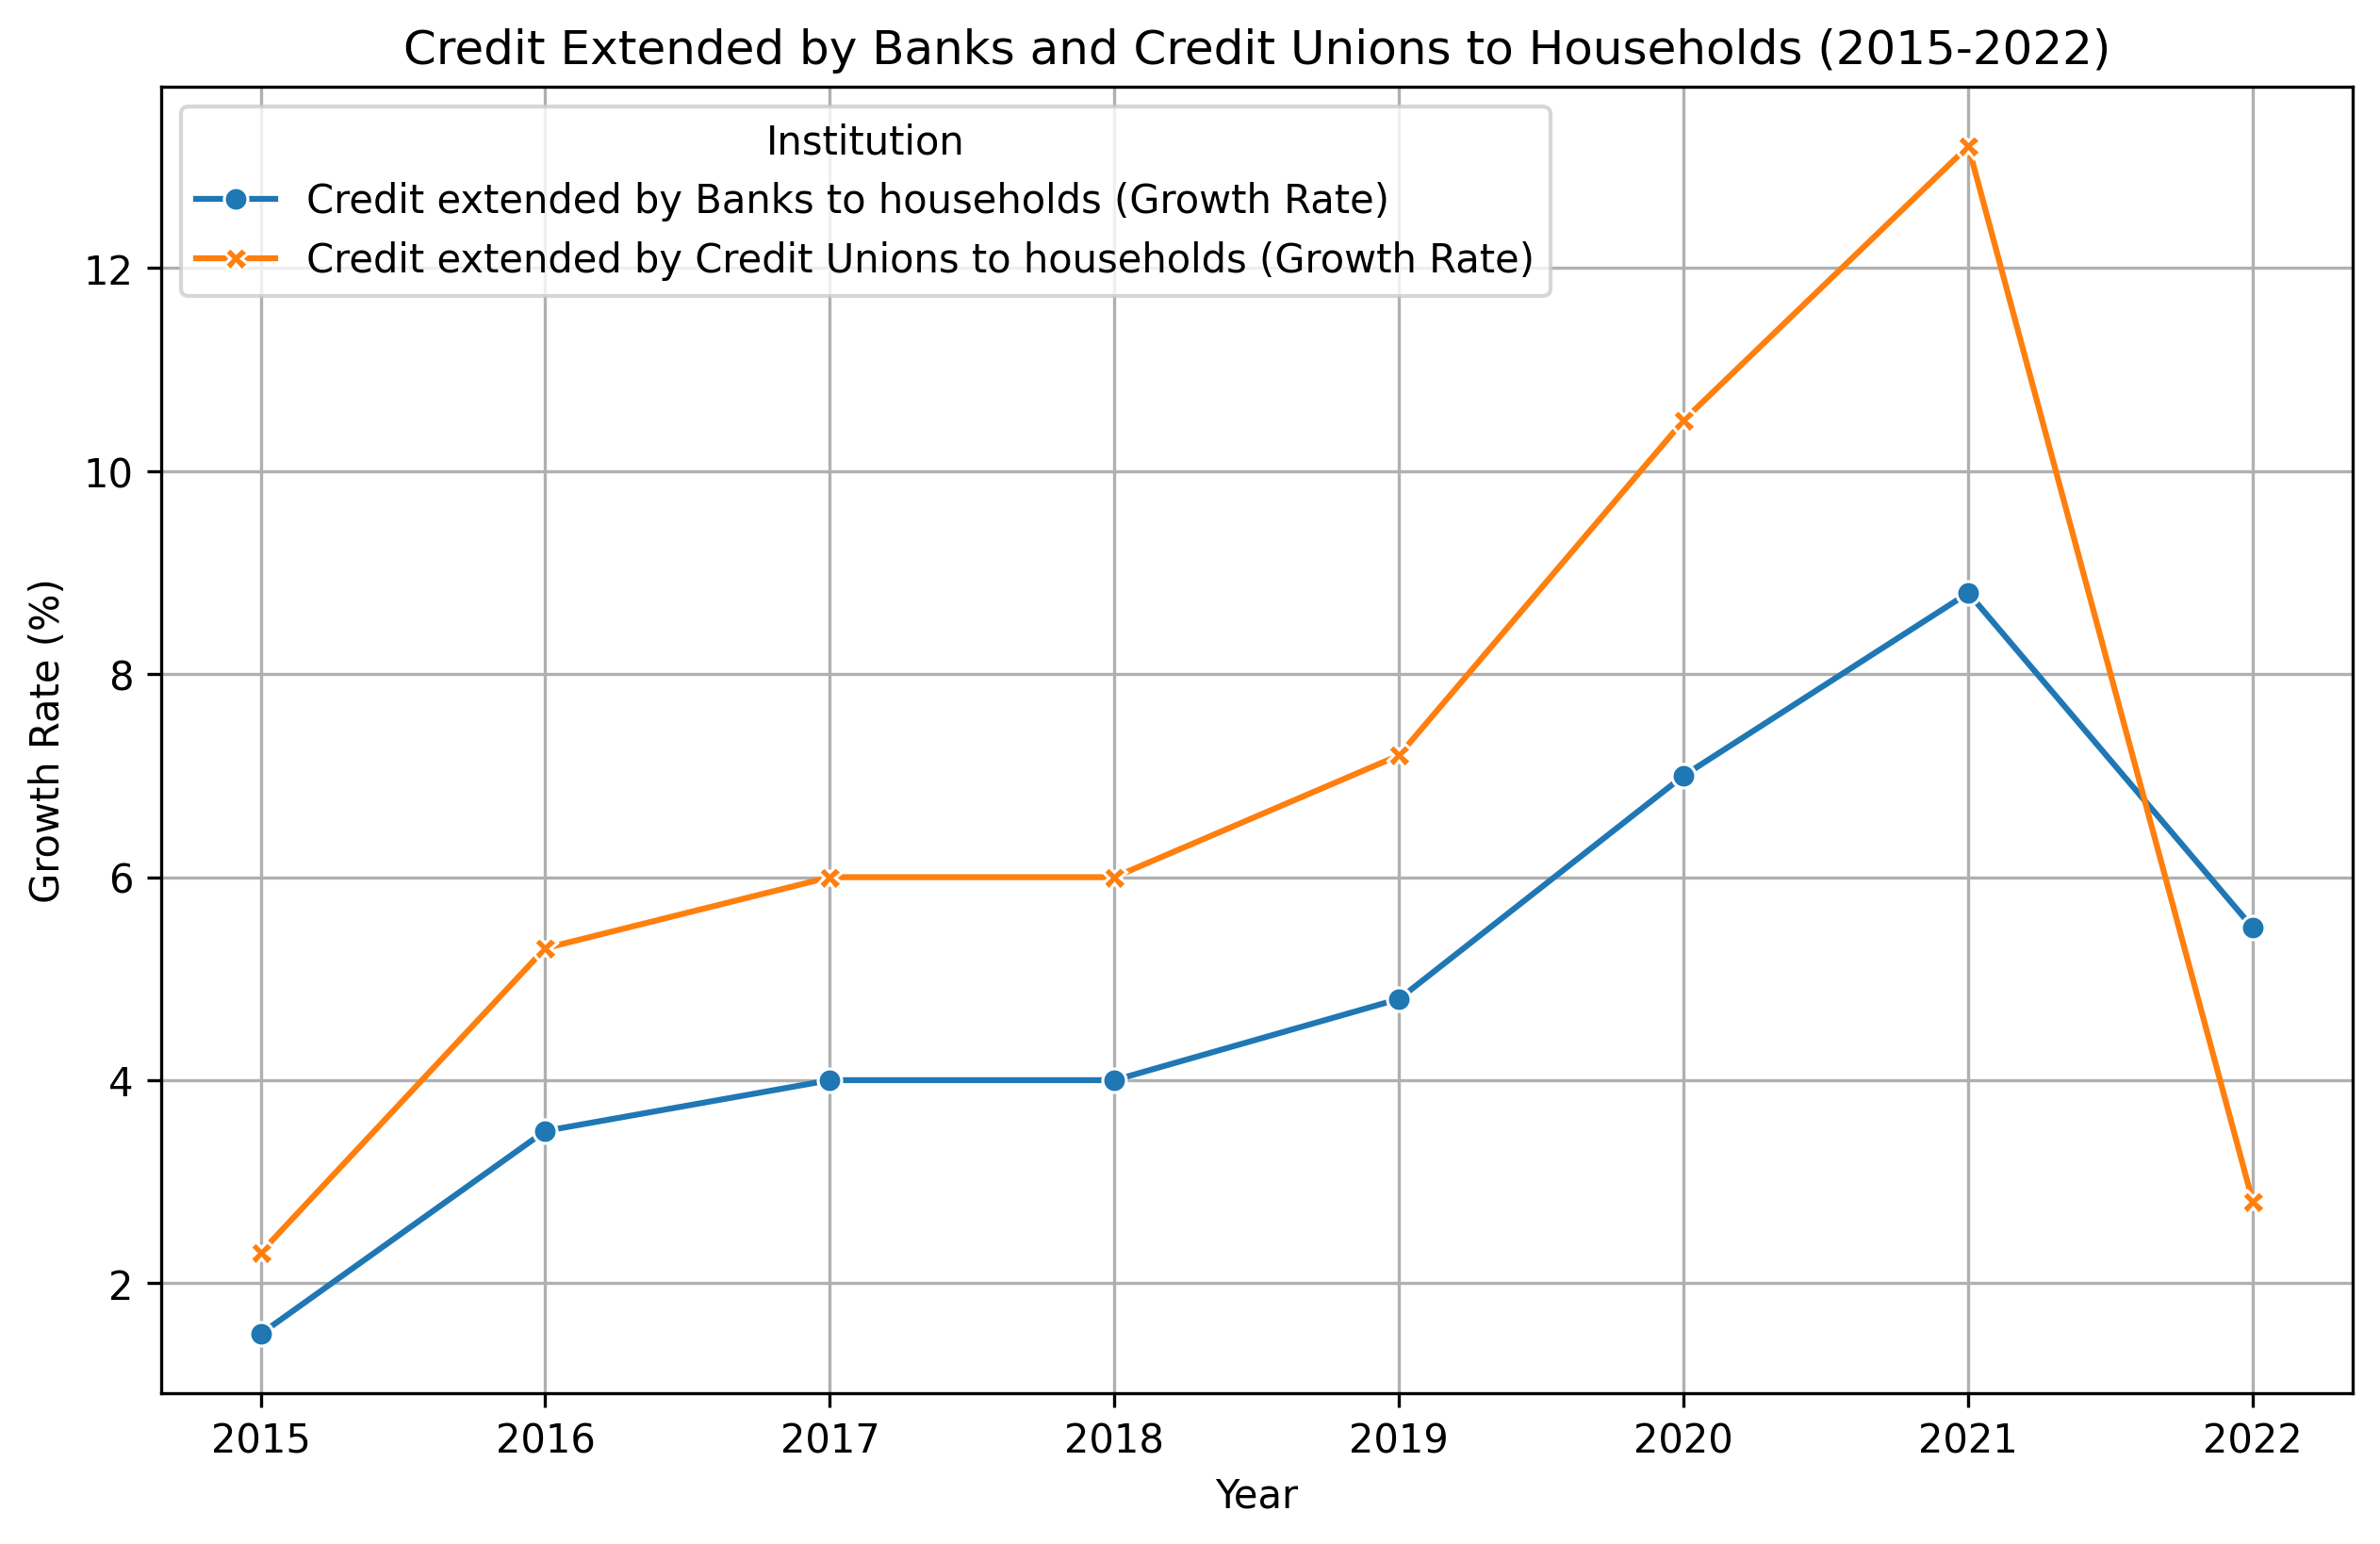
\includegraphics[width=0.8\textwidth]{graph_1.png}
     \caption{Credit Extended By Banks and Credit Unions to Households (2015 - 2022)}
     \label{fig:graph_1}
\end{figure}


\subsection*{Weak Financial Regulation and Insufficient Liquidity}

Macaronia's financial sector suffers from inadequate regulatory oversight, particularly in the near-bank financial sector. This lack of stringent regulation has allowed commercial banks and credit unions to engage in \textcolor{teal}{\textbf{high-risk lending practices}}, such as issuing subprime mortgages and accumulating excessive exposure to volatile real estate markets. The collapse of two commercial banks due to poor capitalization highlights the fragility of the financial system.

The correlation between liquidity ratios and prudential capital adequacy benchmarks (0.59) suggests that weak financial oversight has resulted in \textcolor{teal}{\textbf{undercapitalized banks}}, leaving them vulnerable to economic shocks. Furthermore, the strong correlation between credit extended by banks (0.88) and credit unions (0.81) with solvency ratios underscores how unchecked aggressive lending has weakened financial institutions, jeopardizing their solvency. The high correlation between public debt to GDP and unemployment (0.82) indicates that weak oversight has contributed to an overleveraged public sector, further destabilizing the economy.

For example, the lack of stringent capital requirements has allowed banks to operate with thin capital buffers, making them susceptible to sudden shocks. Additionally, the absence of robust stress-testing mechanisms has left regulators ill-prepared to anticipate and mitigate \textcolor{teal}{\textbf{systemic risks}}. This regulatory gap has created an environment where financial institutions prioritize short-term profits over long-term stability, leading to excessive risk-taking and financial fragility.

\newpage

\subsection*{Ratios Above Benchmarks on Paper, but Insufficient Liquidity}

\begin{figure}[h]
    \centering
    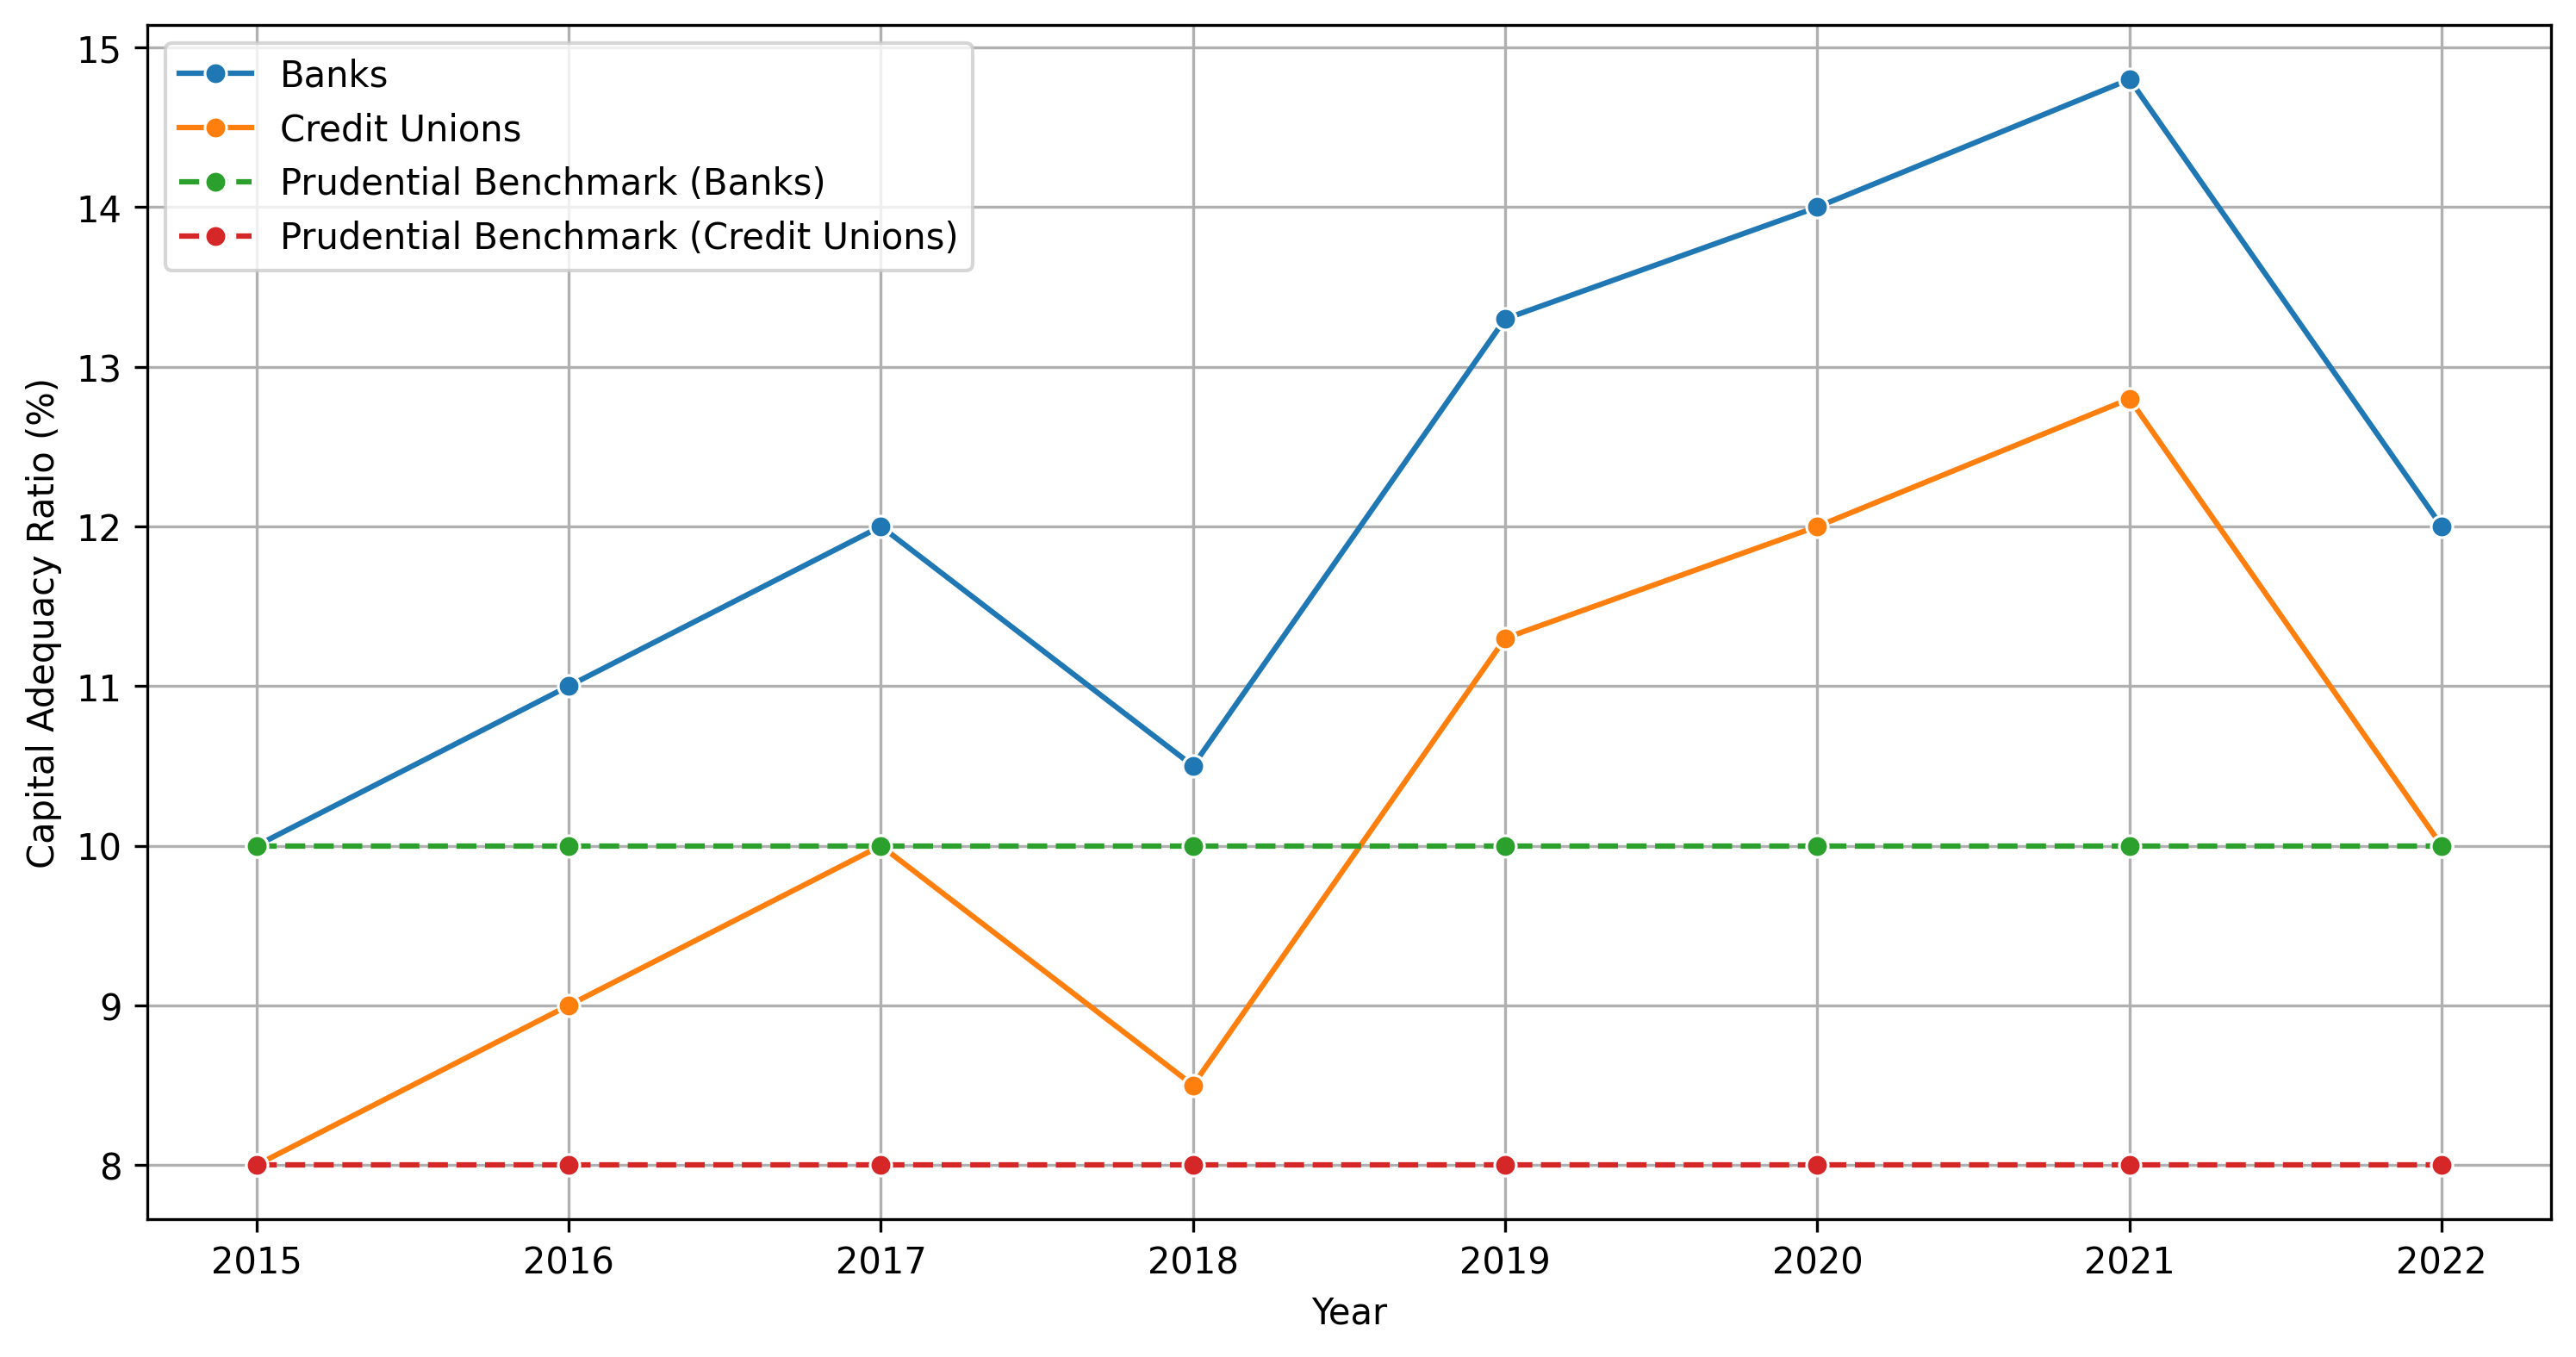
\includegraphics[width=0.8\textwidth]{Benchmarks.png}
    \caption{Credit Extended By Banks and Credit Unions to Households (2015 - 2022)}
    \label{fig:graph_1}
\end{figure}

While the \textbf{liquidity ratios} and \textbf{capital adequacy ratios} for both banks and credit unions are above the prudential benchmarks on paper, the \textbf{credit extension data} reveals a different story. On the surface, the ratios suggest that financial institutions are solvent and have sufficient liquidity to meet short-term obligations:
\begin{itemize}
    \item \textbf{Liquidity Ratios}:
        \begin{itemize}
            \item Banks: 50.0\% to 75.0\% (benchmark: 60.0\%)
            \item Credit Unions: 52.5\% to 78.8\% (benchmark: 50.0\%)
        \end{itemize}
    \item \textbf{Capital Adequacy Ratios}:
        \begin{itemize}
            \item Banks: 10.0\% to 14.8\% (benchmark: 10.0\%)
            \item Credit Unions: 8.0\% to 12.8\% (benchmark: 8.0\%)
        \end{itemize}
\end{itemize}

However, these ratios may not be sufficient to support the \textbf{scale of credit extension} in a high-risk environment like Macaronia's real estate market. Despite meeting the prudential benchmarks, the financial system is under significant strain due to \textbf{aggressive lending practices}:
\begin{itemize}
    \item \textbf{Aggressive Lending}: Banks and credit unions have extended substantial amounts of credit to households, particularly in the real estate sector. For example:
        \begin{itemize}
            \item Credit extended by banks grew from \textbf{1.5\% in 2015 to 8.8\% in 2021}.
            \item Credit extended by credit unions grew from \textbf{2.3\% in 2015 to 13.2\% in 2021}.
        \end{itemize}
    \item \textbf{High-Risk Exposure}: A large portion of this credit is tied to \textbf{high-risk mortgages} and \textbf{Real Estate Investment Trusts (REITs)}, which are highly volatile and sensitive to economic shocks.
\end{itemize}

\subsection*{Insufficient Liquidity to Support Credit Extension}

While the liquidity ratios are above the prudential benchmarks, they fall short of \textbf{international standards} required to support the level of credit extension in a high-risk environment:
\begin{itemize}
    \item According to the \textbf{Basel III framework}, banks should maintain a \textbf{Liquidity Coverage Ratio (LCR)} of at least \textbf{100\%}. This means banks must hold enough high-quality liquid assets to cover their net cash outflows for 30 days.
    \item In Macaronia's case, the liquidity ratios (50.0\% to 75.0\% for banks and 52.5\% to 78.8\% for credit unions) are \textbf{below the recommended 100\% threshold}, indicating that the financial system may not have sufficient liquidity to withstand a sudden surge in withdrawals or a sharp decline in asset values.
\end{itemize}

\subsection*{Weak Financial Regulation}

The fact that financial institutions are meeting the prudential benchmarks but still engaging in \textbf{high-risk lending} and facing \textbf{liquidity shortages} highlights the \textbf{weakness of the regulatory framework}:
\begin{itemize}
    \item \textbf{Lack of Enforcement}: Regulators may not be enforcing the benchmarks effectively, allowing banks and credit unions to operate with thin liquidity buffers.
    \item \textbf{Inadequate Stress Testing}: The absence of robust stress-testing mechanisms means that the institutions may not be prepared for severe economic shocks, such as a collapse in the real estate market.
    \item \textbf{Moral Hazard}: The presence of deposit insurance may have encouraged banks to take excessive risks, knowing that deposits are insured.
\end{itemize}

\subsection*{References to International Standards}

\begin{itemize}
    \item \textbf{Basel III Liquidity Coverage Ratio (LCR)}:
        \begin{itemize}
            \item The Basel III framework requires banks to maintain a \textbf{Liquidity Coverage Ratio (LCR)} of at least \textbf{100\%}. This means banks must hold enough high-quality liquid assets to cover their net cash outflows for 30 days.
            \item Source: \href{https://www.bis.org/bcbs/basel3.htm}{Bank for International Settlements (BIS)}
        \end{itemize}
    \item \textbf{Liquidity Ratios in High-Risk Environments}:
        \begin{itemize}
            \item In economies with high credit growth and exposure to volatile sectors, liquidity ratios should be \textbf{significantly higher} than the minimum benchmarks to account for increased risk.
            \item Source: \href{https://www.imf.org/en/Publications/WP/Issues/2016/12/31/Liquidity-Risk-and-Credit-in-the-Transmission-of-Monetary-Policy-24322}{International Monetary Fund (IMF)}
        \end{itemize}
\end{itemize}

\newpage

\subsection*{Overreliance on the Real Estate Sector}

Macaronia’s economic growth has been heavily dependent on its booming real estate market. Commercial banks and credit unions have significantly exposed themselves to Real Estate Investment Trusts (REITs), with 15\% and 25\% of their total assets tied to these instruments, respectively. However, REITs are highly volatile, particularly during economic shocks, and rely heavily on debt to finance property acquisitions and developments. They also have limited economic growth potential, tax implications, and sensitivity to interest rate fluctuations. As REIT values decline sharply, the balance sheets of financial institutions deteriorate. This erosion of equity can lead to \textcolor{teal}{\textbf{insolvency}}, limiting the institutions’ ability to lend and slowing economic activity.

The high correlations between credit extended by banks to households (0.88) and credit unions (0.81) with solvency ratios demonstrate that real estate-driven lending has been a primary factor in the financial health of banks and credit unions. The correlation between economic growth and credit union lending (0.77) underscores how the real estate boom has fueled Macaronia’s GDP expansion. However, the liquidity ratios of banks (0.61) and credit unions (0.75) alongside inflation reveal that inflationary pressures have emerged alongside credit expansion, further straining the economy. 

With REIT values declining sharply, highly leveraged banks and credit unions now face significant balance sheet deterioration, threatening their stability.

\subsection*{Aggressive Lending Practices and Economic Instability}

Aggressive lending practices have been a hallmark of Macaronia’s financial sector, driven by the real estate boom. However, this credit-fueled expansion has proven unsustainable, contributing to inflationary pressures and weakening bank balance sheets. The correlation between bank and credit union lending with economic growth (0.77) indicates that economic growth has been heavily reliant on unsustainable credit expansion. Excessive credit growth has also contributed to rising inflation, as evidenced by the correlation between liquidity ratios and inflation (0.61), further destabilizing the economy. Moreover, the strong correlation between banks’ lending and capital adequacy (0.88) shows that aggressive lending practices have directly weakened bank balance sheets, increasing systemic risk.

For example, banks have extended loans to borrowers with poor creditworthiness, often without adequate collateral. This has increased the risk of defaults, particularly in a deteriorating economic environment. Additionally, the lack of diversification in loan portfolios has left banks overly exposed to the real estate sector, amplifying the impact of sector-specific shocks.

\subsection{Currency Instability}

Macaronia’s currency has experienced significant depreciation, driven by a combination of fiscal deficits, liquidity shortages, and inflationary pressures. This instability has further exacerbated the economic crisis. The negative correlation between the exchange rate and inflation (-0.85) indicates that currency depreciation is fueling inflation, likely due to higher import costs. Persistent fiscal deficits are also driving currency instability, as shown by the correlation between fiscal deficit and exchange rate (-0.37), undermining investor confidence. Additionally, liquidity shortages are worsening currency volatility, as evidenced by the correlation between liquidity ratios and exchange rate (-0.28), creating a vicious cycle of economic instability.
For instance, the depreciation of the currency has led to a surge in the cost of imported goods, further straining household budgets and reducing consumer spending. This has had a knock-on effect on businesses, particularly those reliant on imported inputs, leading to reduced production and layoffs.haken depositor trust.

\subsection{Depositor Confidence Erosion}


The erosion of depositor confidence is a critical issue, as it threatens to trigger bank runs and further destabilize the financial system.
Declining solvency ratios and public debt concerns have shaken depositor trust. The high correlation between liquidity ratios and solvency ratios (0.94) 
suggests that depositors are withdrawing funds due to declining solvency, exacerbating liquidity issues. Depositor confidence is further undermined by concerns 
over high public debt levels, as indicated by the correlation between public debt to GDP and exchange rate (-0.68). Financial distress, reflected in the stock market decline, 
is eroding overall economic stability, as depositors and investors lose faith in the financial system.
For example, the recent collapse of two major banks has led to widespread panic among depositors, resulting in a surge in withdrawals. 
This has forced banks to liquidate assets at distressed prices, further weakening their financial position and creating a downward spiral.

%
\newpage
 

\subsection*{Financial Health}

\begin{figure}[h]
    \centering
    \begin{subfigure}{0.48\textwidth}
        \centering
        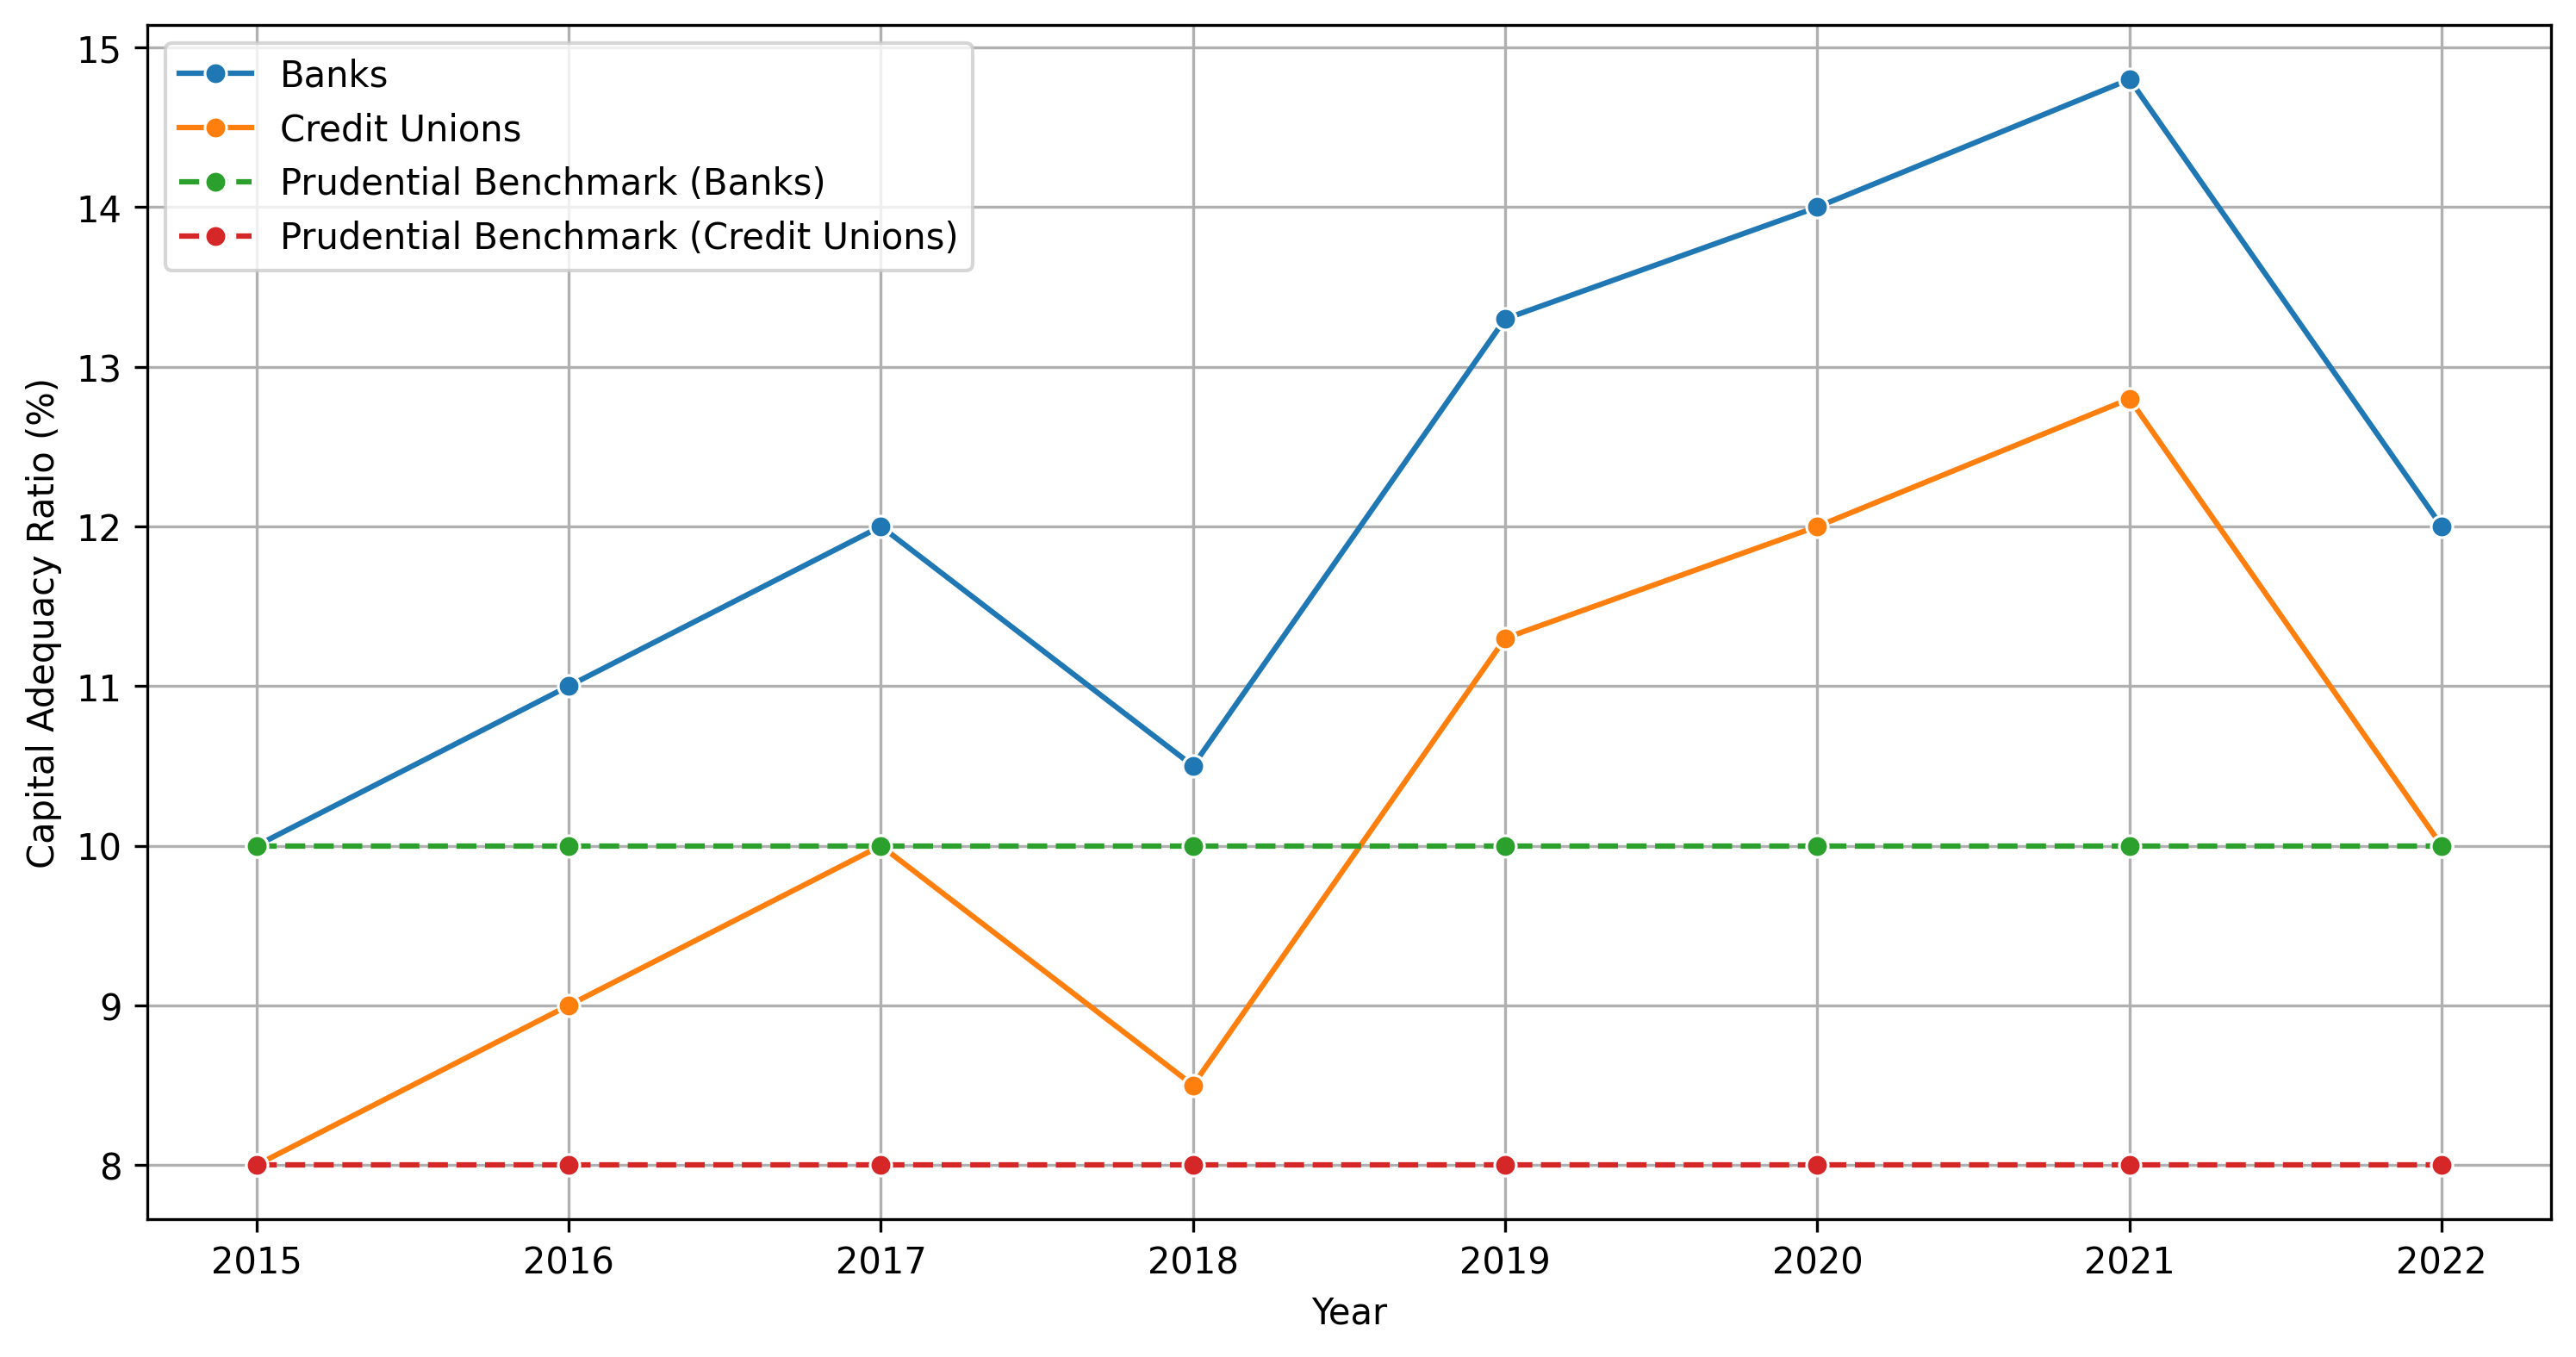
\includegraphics[width=\textwidth]{Benchmarks.png}
        \caption{\small Credit Extended by Banks and Credit Unions}
        \label{fig:benchmarks}
    \end{subfigure}
    \hfill
    \begin{subfigure}{0.48\textwidth}
        \centering
        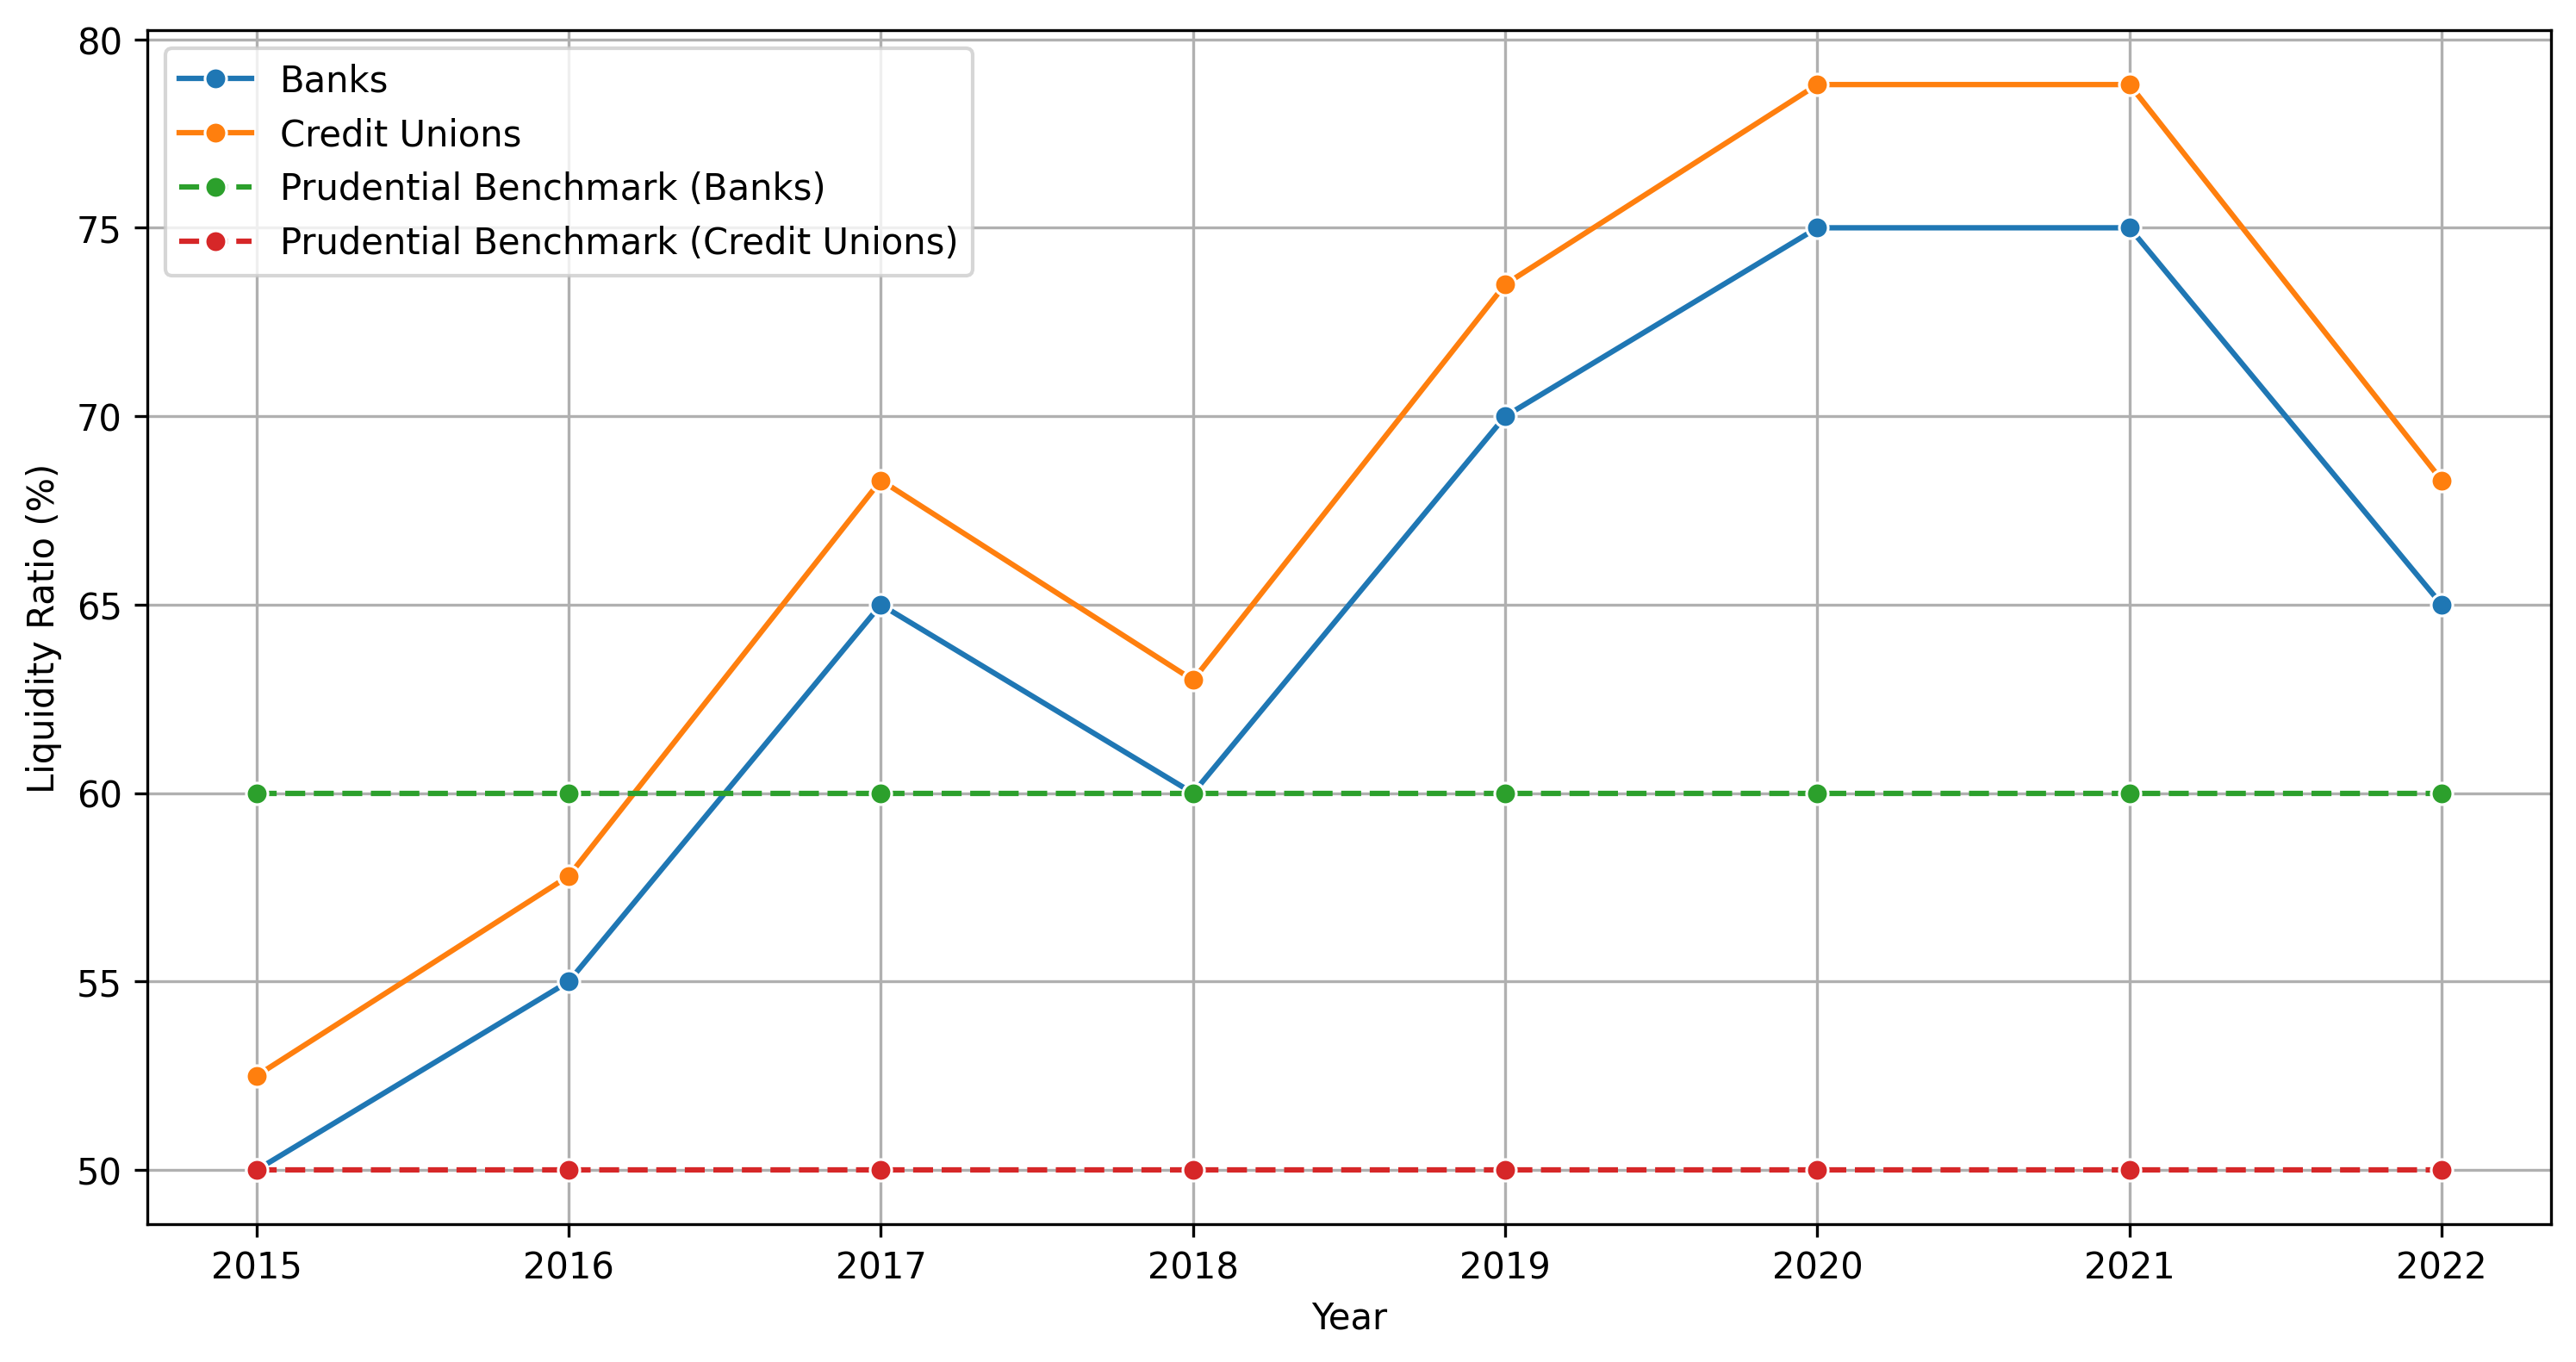
\includegraphics[width=\textwidth]{liquidity_ratio.png}
        \caption{\small Liquidity Ratios for Banks and Credit Unions}
        \label{fig:liquidity_ratios}
    \end{subfigure}
    \caption{Banking Sector Credit and Liquidity Ratios}  % Main figure caption
    \label{fig:credit_liquidity}
\end{figure}



Nominally, Macaronia's \textcolor{teal}{liquidity} and \textcolor{teal}{capital adequacy ratios} are both above the set \textcolor{teal}{prudential benchmarks}.  
Over the years, \textcolor{teal}{banks} and \textcolor{teal}{credit unions} have attained \textcolor{teal}{liquidity ratios} of \textbf{\textcolor{teal}{75\%}} (a \textbf{\textcolor{teal}{25\% increase}})  
and \textbf{\textcolor{teal}{78.8\%}} (a \textbf{\textcolor{teal}{26.3\% increase}}), respectively.  
Similarly, \textcolor{teal}{capital adequacy ratios} have reached \textbf{\textcolor{teal}{14.8\%}} (a \textbf{\textcolor{teal}{4.8\% increase}}) for \textcolor{teal}{banks}  
and \textbf{\textcolor{teal}{12.8\%}} (a \textbf{\textcolor{teal}{4.8\% increase}}) for \textcolor{teal}{credit unions}.  
On paper, these ratios appear strong, suggesting that \textcolor{teal}{financial institutions} are \textcolor{teal}{solvent}  
and have sufficient \textcolor{teal}{liquidity} to meet \textcolor{teal}{short-term obligations}.


However, much like inflation erodes the real value of money, the effectiveness of these ratios is being 
undermined by the rapid expansion of credit. While the ratios are rising, the scale of credit being extended 
to Macaronia's households has grown at a significant rate as well. For instance:

\begin{itemize}
    \item \textbf{\textcolor{teal}{Credit extended by banks}} grew from \textbf{\textcolor{teal}{1.5\% in 2015}} to \textbf{\textcolor{teal}{8.8\% in 2021}}.
    \item \textbf{\textcolor{teal}{Credit extended by credit unions}} grew from \textbf{\textcolor{teal}{2.3\% in 2015}} to \textbf{\textcolor{teal}{13.3\% in 2021}}.
\end{itemize}

This rapid growth in credit is evidenced by the strong correlations between 
\textbf{credit extended by banks (0.92)} and \textbf{credit unions (0.86)} with their respective 
solvency ratios, as well as between \textbf{credit extended by banks (0.91)} and \textbf{credit unions (0.81)} 
with their respective liquidity ratios.

\begin{figure}[h]     
     \centering
     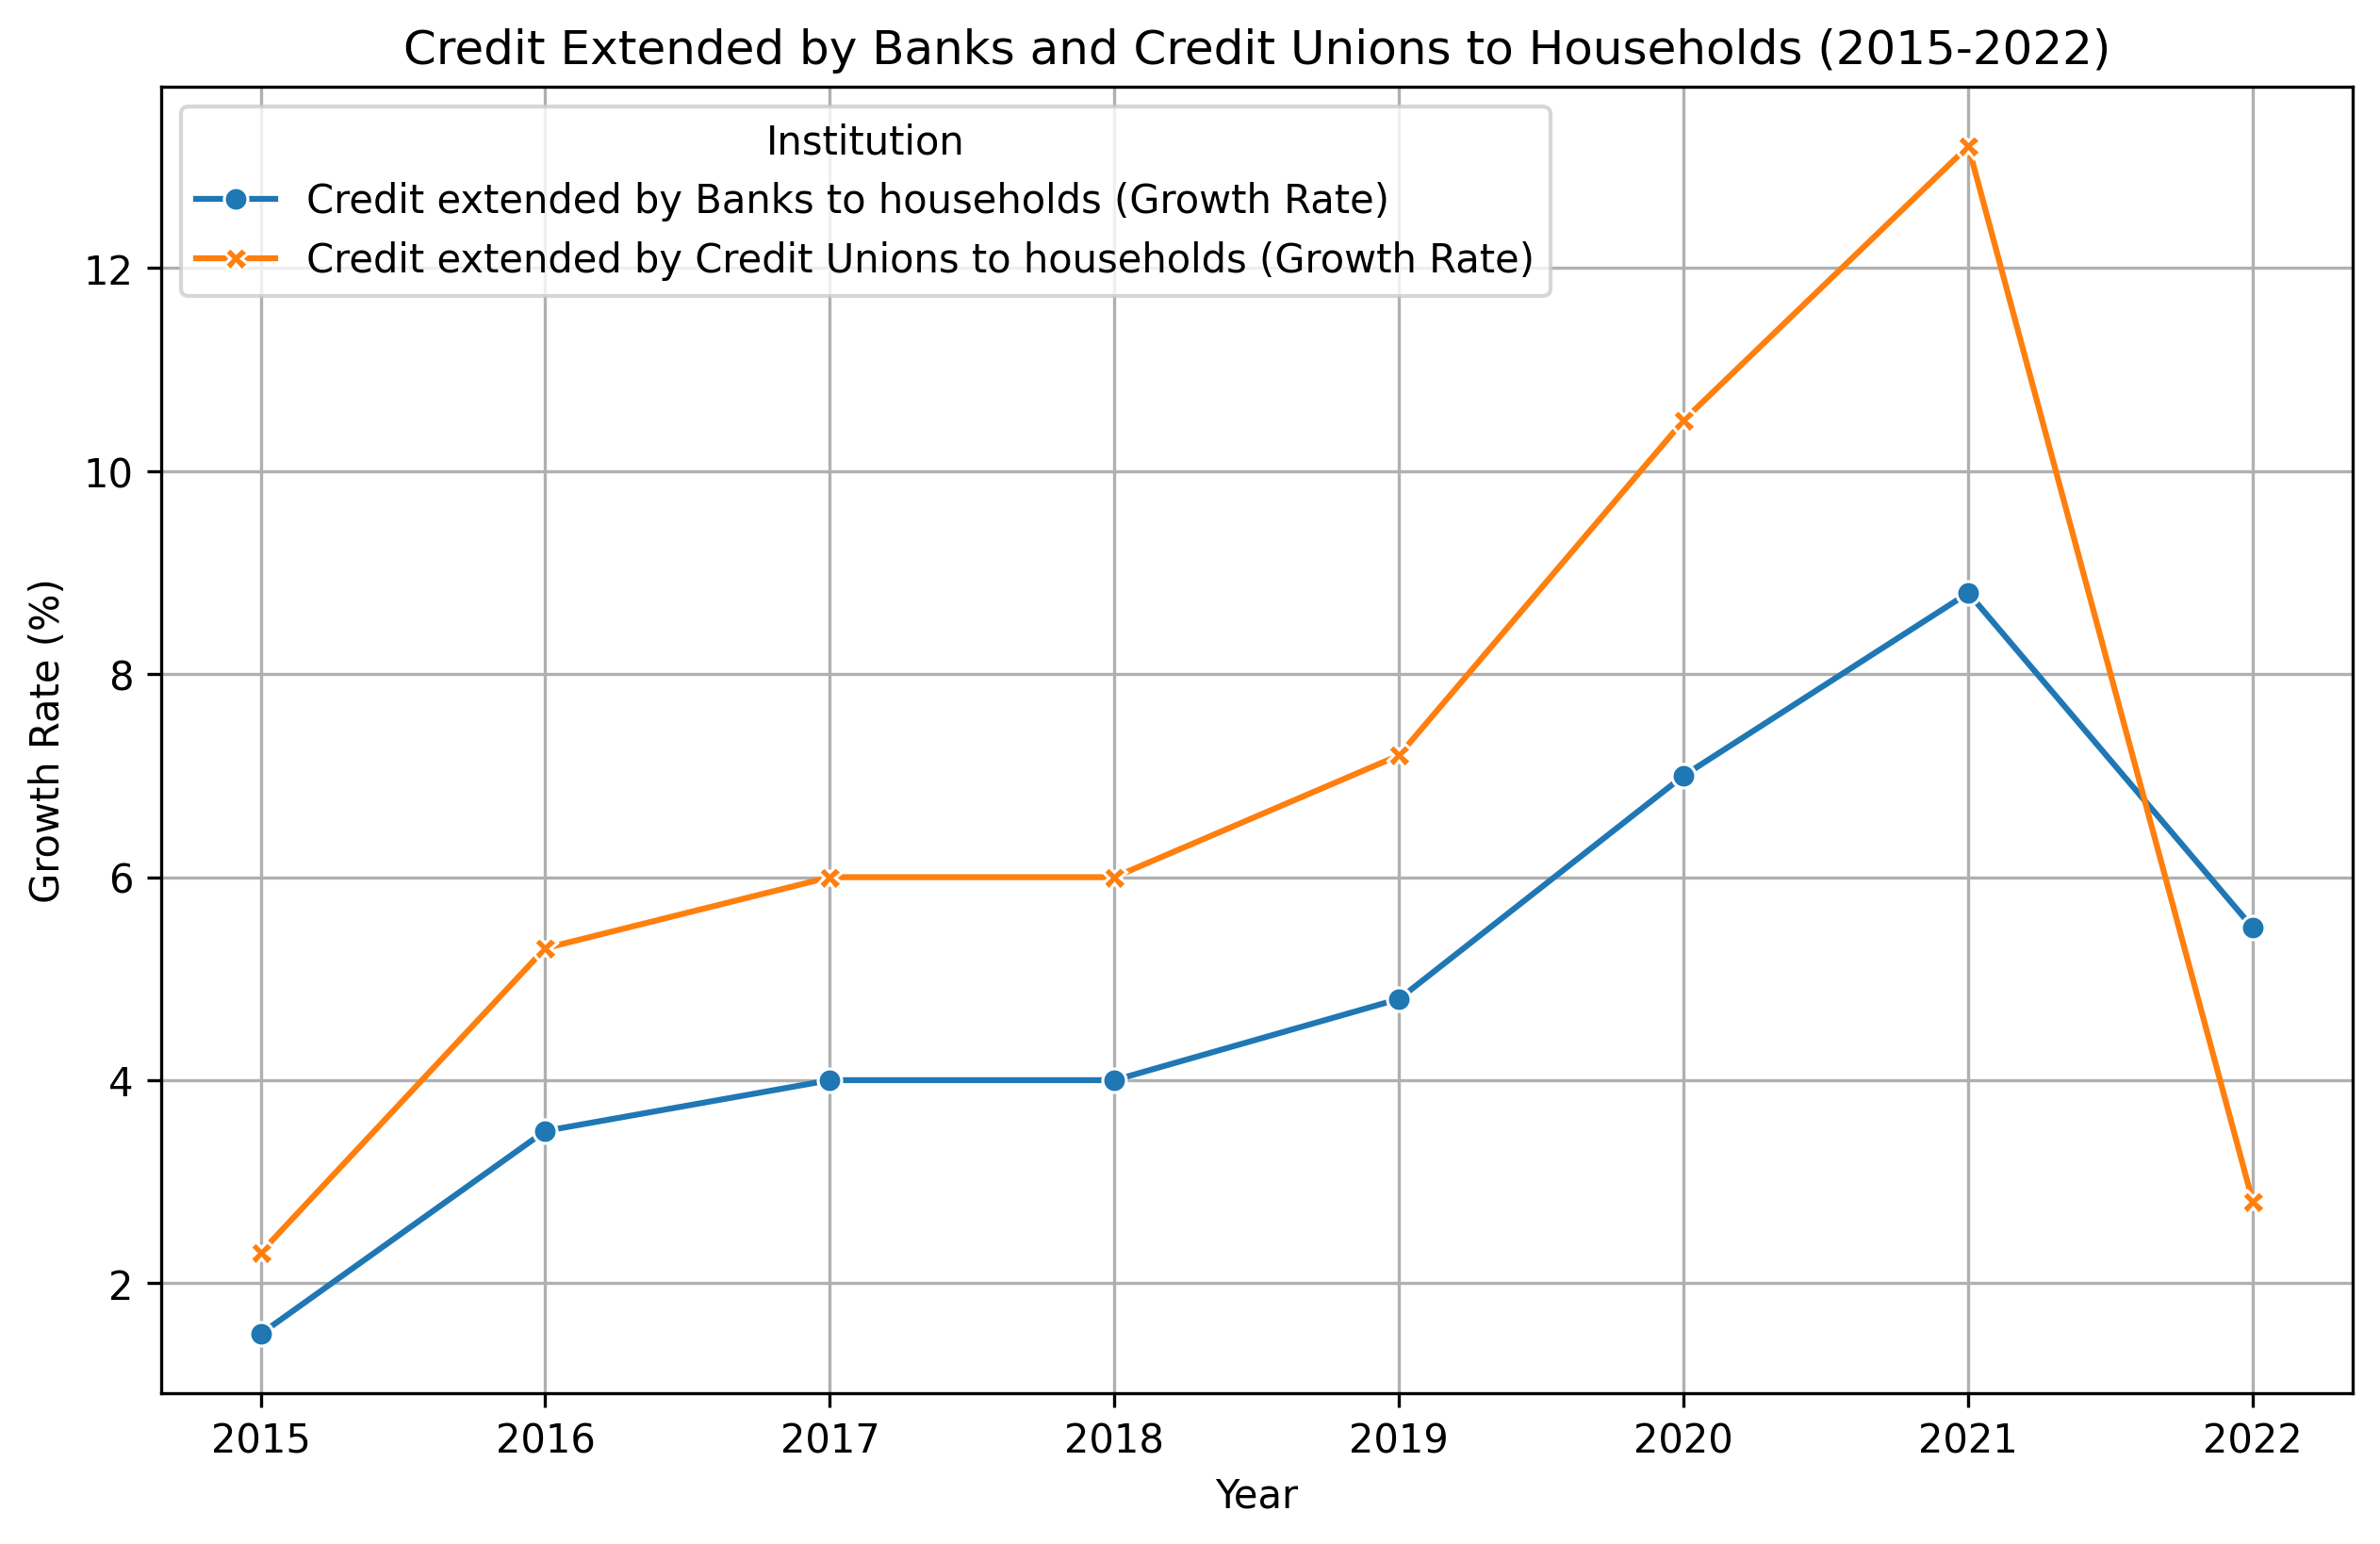
\includegraphics[width=0.53\textwidth]{graph_1.png}
     \caption{Credit Extended By Banks and Credit Unions to Households (2015 - 2022)}
     \label{fig:graph_1}
\end{figure}

To make matters worse, both banks and credit unions in Macaronia are heavily exposed to \textbf{\textcolor{teal}{Real Estate Investment Trusts (REITs)}}, 
with banks having \textbf{\textcolor{teal}{15\%}} of their assets tied to REITs, and credit unions having \textbf{\textcolor{teal}{25\%}}. 
REITs are highly volatile, with their values subject to significant fluctuations based on market conditions, 
interest rates, and economic cycles. In times of economic uncertainty, these assets put financial institutions
in a precarious position, as they would struggle to meet their short-term obligations in the event of a bank run
or an external shock.  \textcolor{orange}{\cite{FSB2023GlobalMonitoring}}


\begin{figure}[h]
    \centering
    \begin{subfigure}{0.48\textwidth}
        \centering
        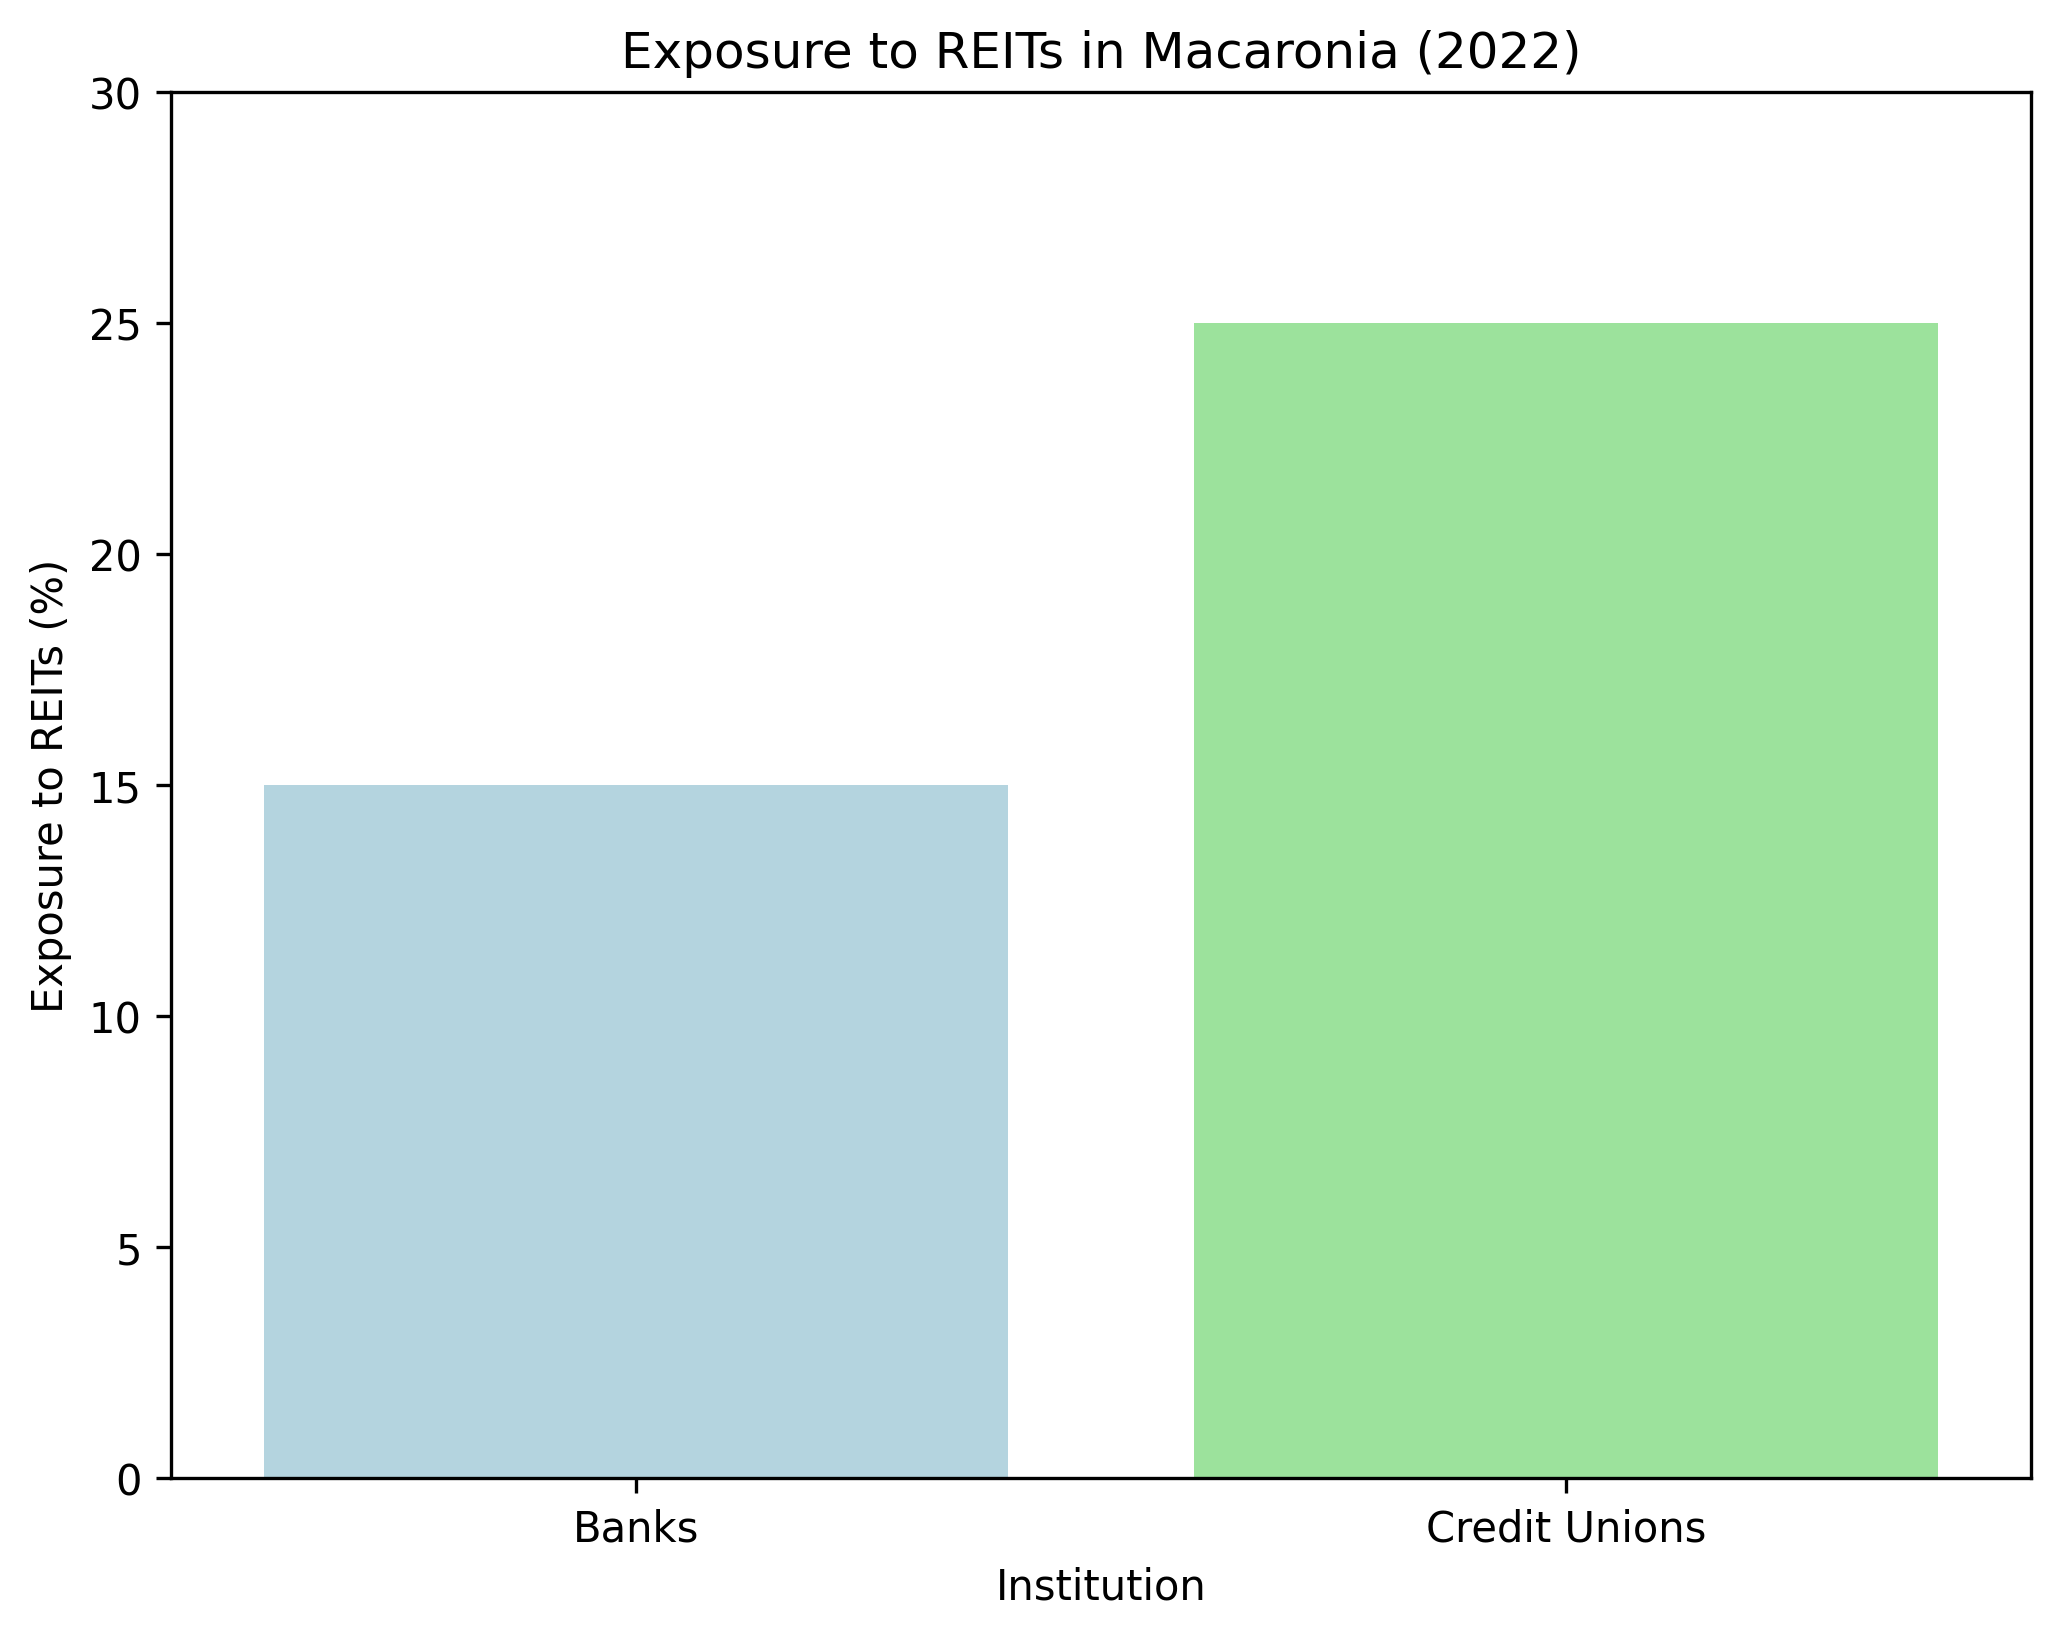
\includegraphics[width=\textwidth]{REIT.png}
        \caption{\small REIT Exposure}
        \label{fig:reit_exposure}
    \end{subfigure}
    \hfill
    \begin{subfigure}{0.48\textwidth}
        \centering
        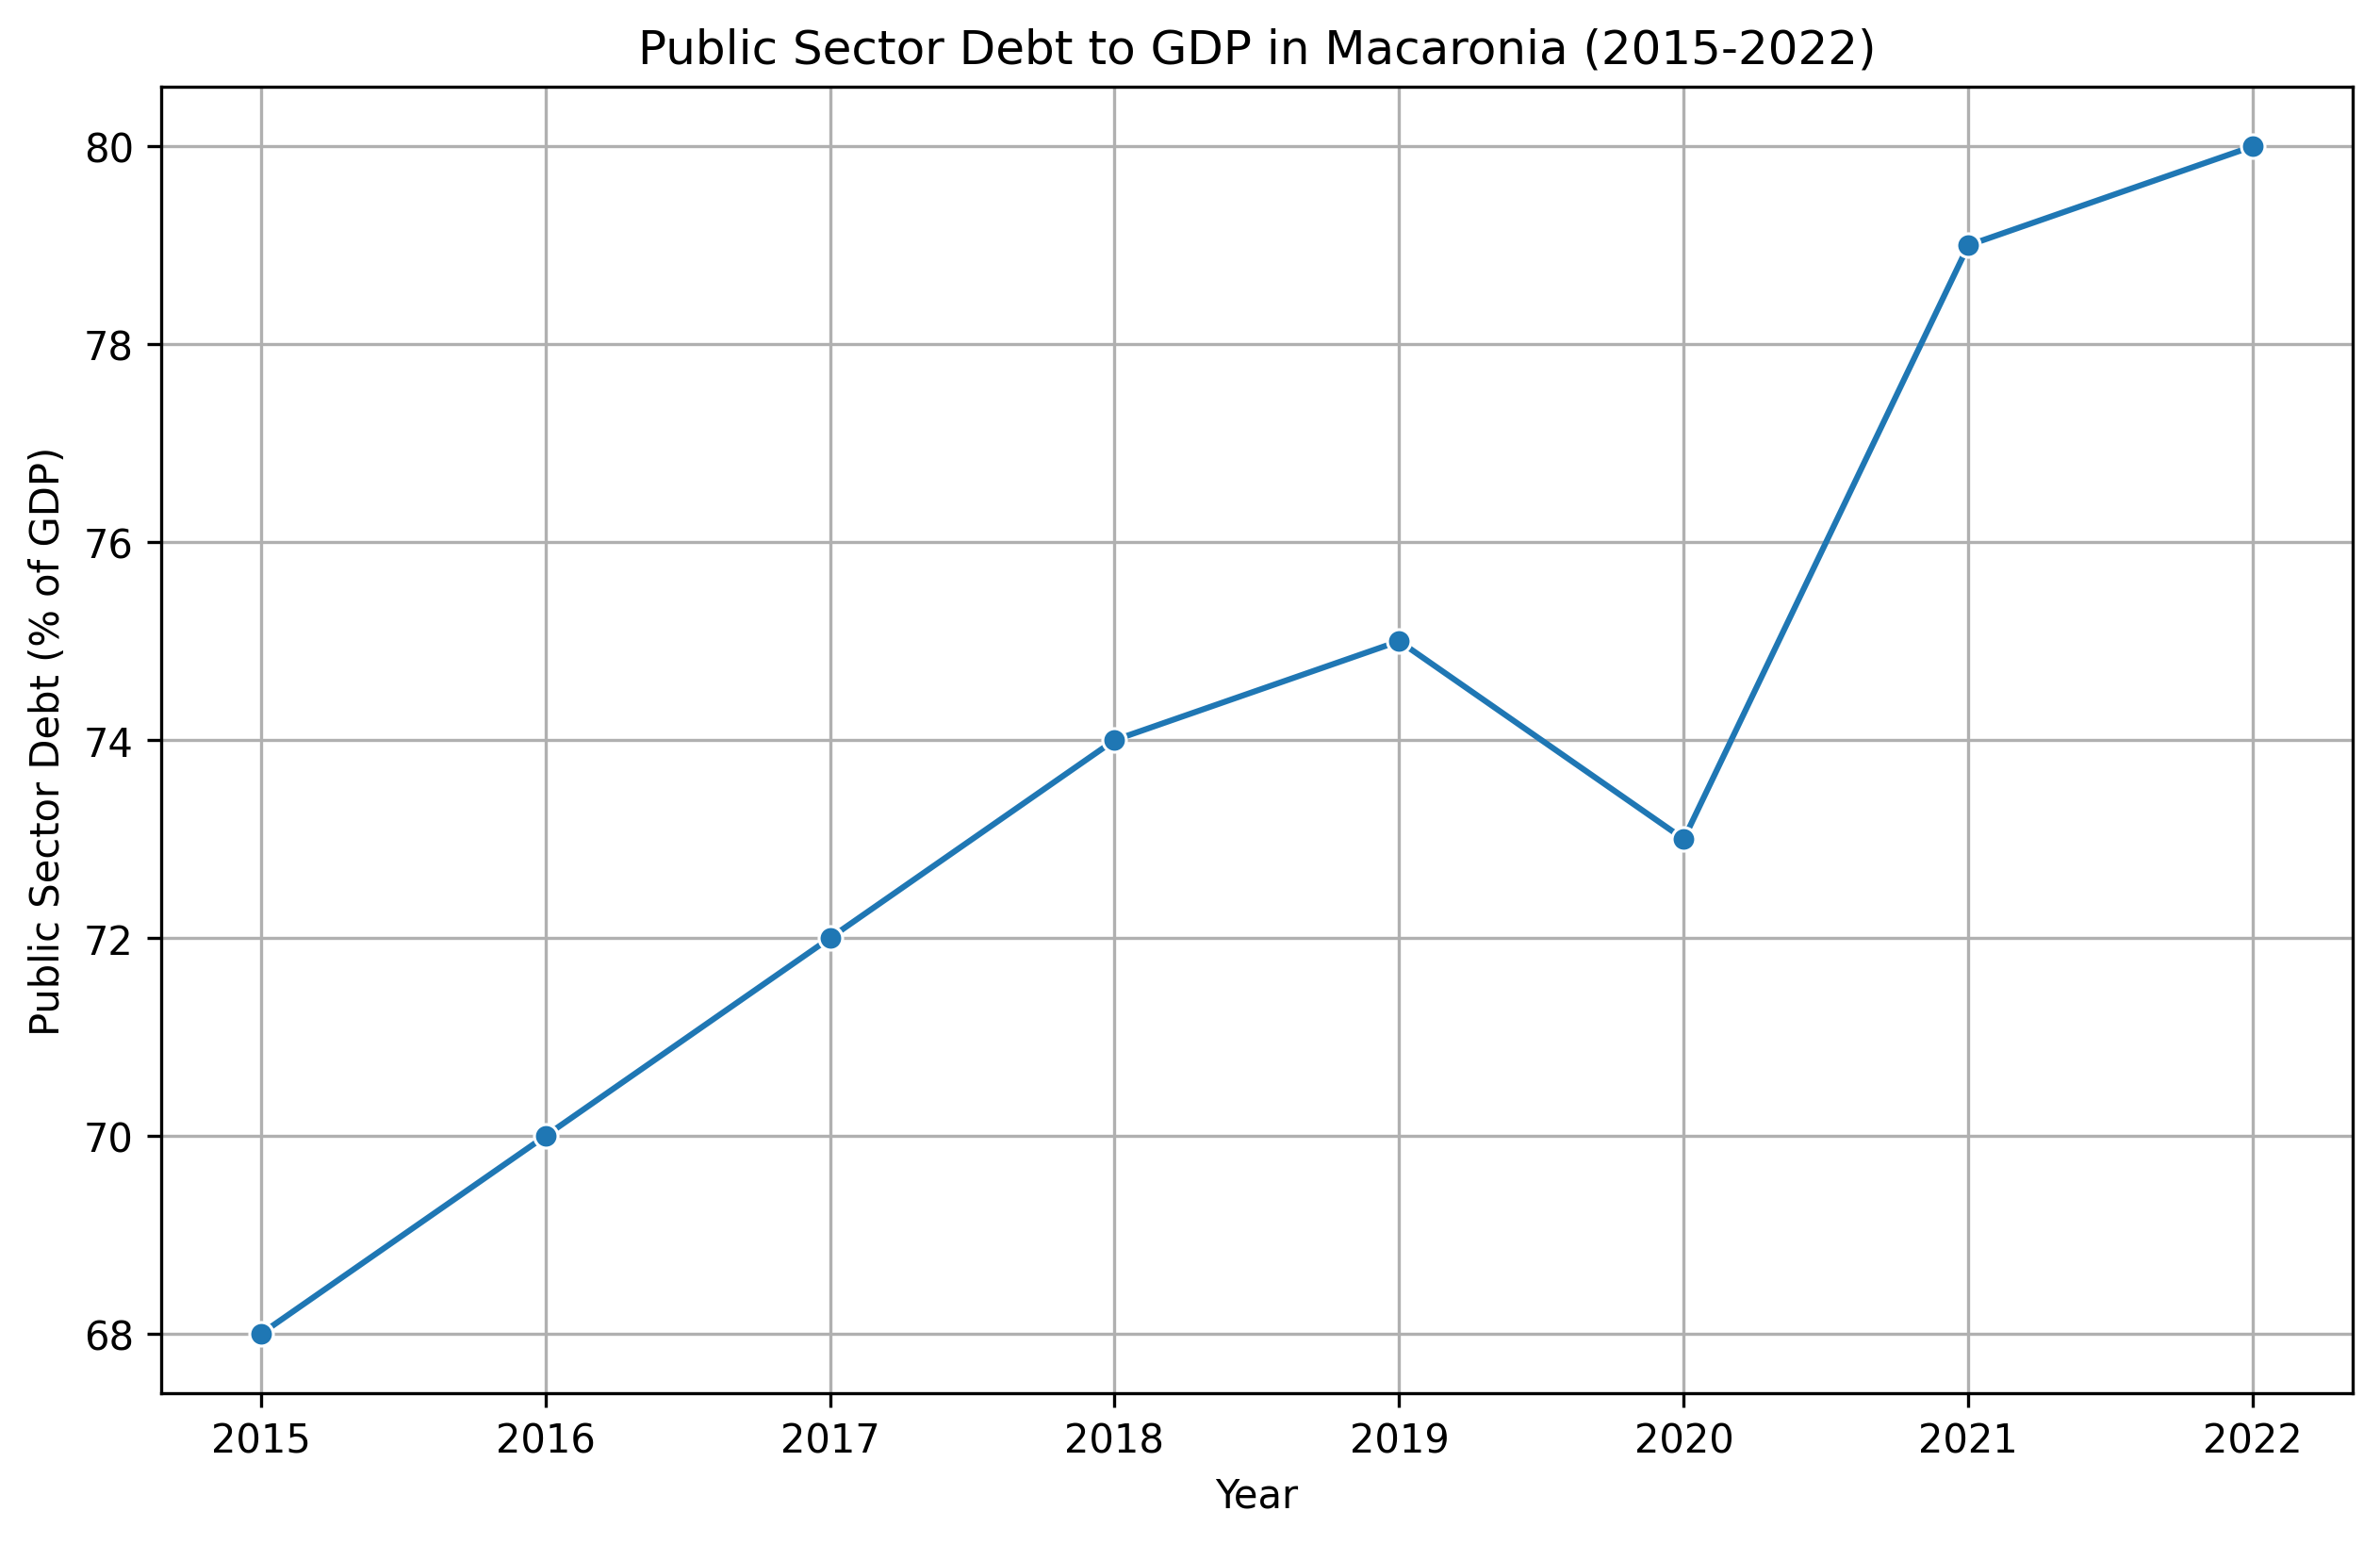
\includegraphics[width=\textwidth]{graph_2.png}
        \caption{\small Public Debt to GDP}
        \label{fig:public_debt_gdp}
    \end{subfigure}
    \caption{Macaronia's REIT Exposure and Public Debt Levels}  % Main figure caption
    \label{fig:reit_debt}
\end{figure}


Given that \textbf{\textcolor{teal}{REITs}} constitute a significant portion of their equity, the risk of \textbf{\textcolor{teal}{insolvency}} is 
substantially higher. A market downturn could trigger a sharp decline in the value of these assets,
eroding the financial institutions' capital bases. To mitigate these risks and strengthen their balance sheets, 
these institutions have resorted to aggressive \textbf{\textcolor{teal}{lending practices}}.

However, the public sector's debt level, which stands at a staggering \textbf{\textcolor{teal}{80\%}} of GDP, 
raises serious concerns about the government's capacity to meet its own financial obligations, 
let alone provide \textbf{\textcolor{teal}{bailouts}} to struggling financial institutions in the event of a crisis. 
In light of this precarious fiscal position, it is essential to move beyond nominal ratios and 
assess the true health of financial institutions by accounting for \textbf{\textcolor{teal}{credit extension}}, 
\textbf{\textcolor{teal}{risk}} and \textbf{\textcolor{teal}{REIT exposure}}.

When these nominal ratios are adjusted, their real value is significantly lower than the nominal figures suggest.
This adjustment uncovers the underlying vulnerabilities in the financial system, emphasizing the urgent need for a more 
accurate assessment of \textbf{\textcolor{teal}{solvency}} and \textbf{\textcolor{teal}{liquidity risks}}.

The adjusted ratio is calculated as:
\begin{equation}
\boxed{
    \text{Adjusted Ratio} = \frac{\text{Nominal Ratio}}{\text{Adjustment Factor}}
}
\end{equation}

To reflect the compounding impact of credit growth, risk exposure and REIT exposure, the adjustment factor is: 

The adjustment factor is calculated as:
\begin{equation}
\boxed{
    \text{Adjustment Factor} = (1 + \text{Credit Growth Rate}) \cdot (1 + \text{Risk Exposure Factor}) \cdot (1 + \text{REIT Exposure})
}
\end{equation}


The risk exposure factor is a subjective measure that reflects the level of risk in the financial system due to factors like economic instblity, 
high levels of debt, or exposure to volatile sectors. In this case, the risk exposure factor is assumed to be 0.5 in 2021 due to the rapid 
credit growth, High REIT exposure and Systemic instability. 



\subsubsection*{Calculations for Banks and Credit Unions real ratios} 



% Increase row height
\renewcommand{\arraystretch}{1.5} % Adjust this value to increase/decrease row height

\begin{table}[h!]
\centering
\begin{tabular}{|>{\centering\arraybackslash}p{4cm}|>{\centering\arraybackslash}p{4cm}|>{\centering\arraybackslash}p{4cm}|} % Centered columns
\hline
\textbf{Parameter} & \textbf{Banks} & \textbf{Credit Unions} \\
\hline
Credit Growth Rate & 0.088 (8.8\%) & 0.132 (13.2\%) \\
\hline
Risk Exposure Factor & 0.5 & 0.5 \\
\hline
REIT Exposure & 0.15 & 0.25 \\
\hline
\textbf{Adjustment Factor} & \textbf{Calculation} & \textbf{Calculation} \\
\hline
& \((1 + 0.088) \times (1 + 0.5) \times (1 + 0.15)\) & \((1 + 0.132) \times (1 + 0.5) \times (1 + 0.25)\) \\
& \(= 1.088 \times 1.5 \times 1.15\) & \(= 1.132 \times 1.5 \times 1.25\) \\
& \(= 1.878\) & \(= 2.122\) \\
\hline
\textbf{Adjusted Real Ratios} & \textbf{Calculation} & \textbf{Calculation} \\
\hline
$\text{Real Liquidity Ratio}_{2021}$ & \(75.0/1.878 = 39.94\) & \(78.8/2.122 = 37.14\) \\
\hline
$\text{Real Adequacy Ratio}_{2021}$ & \(14.8/1.878 = 7.88\) & \(12.8/2.122 = 6.03\) \\
\hline
\end{tabular}
\caption{Adjustment Factor and Adjusted Real Ratios for Banks and Credit Unions (2021)}
\end{table}

The real liquidity ratio for banks stands at \textcolor{teal}{39.94}, and for credit unions, it is \textcolor{teal}{37.14}. Similarly, the real solvency ratio for banks is approximately \textcolor{teal}{7.88}, compared to \textcolor{teal}{6.03} for credit unions. While these ratios may appear stable at first glance, the adjusted figures accounting for \textcolor{teal}{credit growth} and \textcolor{teal}{high-risk asset exposure} reveal a far more concerning reality: both banks and credit unions are \textcolor{teal}{undercapitalized}. This imbalance represents a latent threat within the financial system, one that grows more precarious as external pressures mount.

The parallels to the \textcolor{teal}{2007-2009 financial crisis} are hard to ignore. During that period, undercapitalized institutions were unable to absorb losses when the housing market collapsed, setting off a chain reaction that destabilized the global economy. Today, a similar vulnerability exists. Banks and credit unions, which are meant to serve as pillars of economic stability, could instead become conduits for \textcolor{teal}{systemic risk}. In times of economic stress, their weakened positions could transform them from stabilizers into amplifiers of crisis.

A significant contributor to this risk is the heavy reliance of financial institutions on the \textcolor{teal}{volatile real estate market}. During periods of economic expansion, real estate investments can generate substantial returns, masking underlying weaknesses in balance sheets. However, when market conditions deteriorate, these same investments can quickly become liabilities.

This combination of \textcolor{teal}{undercapitalization} and \textcolor{teal}{overexposure to risky assets} creates the potential for a \textcolor{teal}{domino effect}. If a single institution faces a liquidity or solvency crisis, it could set off a chain reaction, destabilizing the broader financial system. The 2007-2009 crisis demonstrated how the collapse of the housing market could trigger a global recession. In the year 2021 in Macaronia, the same dynamics are at play. Financial institutions, weakened by undercapitalization and over-leveraged portfolios, may struggle to withstand the next economic shock, putting the entire financial ecosystem at risk.

The question is not whether this scenario will unfold, but when. This urgency is further amplified by the fact that Macaronia's economy is \textcolor{teal}{perfectly correlated with global economic growth}, with a correlation coefficient of \textcolor{teal}{1}. This means that any downturn or shock in the global economy will have an immediate and proportional impact on Macaronia, leaving its already fragile financial system even more exposed to \textcolor{teal}{external pressures}.
\textcolor{orange}{\cite{UNCTAD2023FDI}}

\begin{figure}[h]
     \centering
     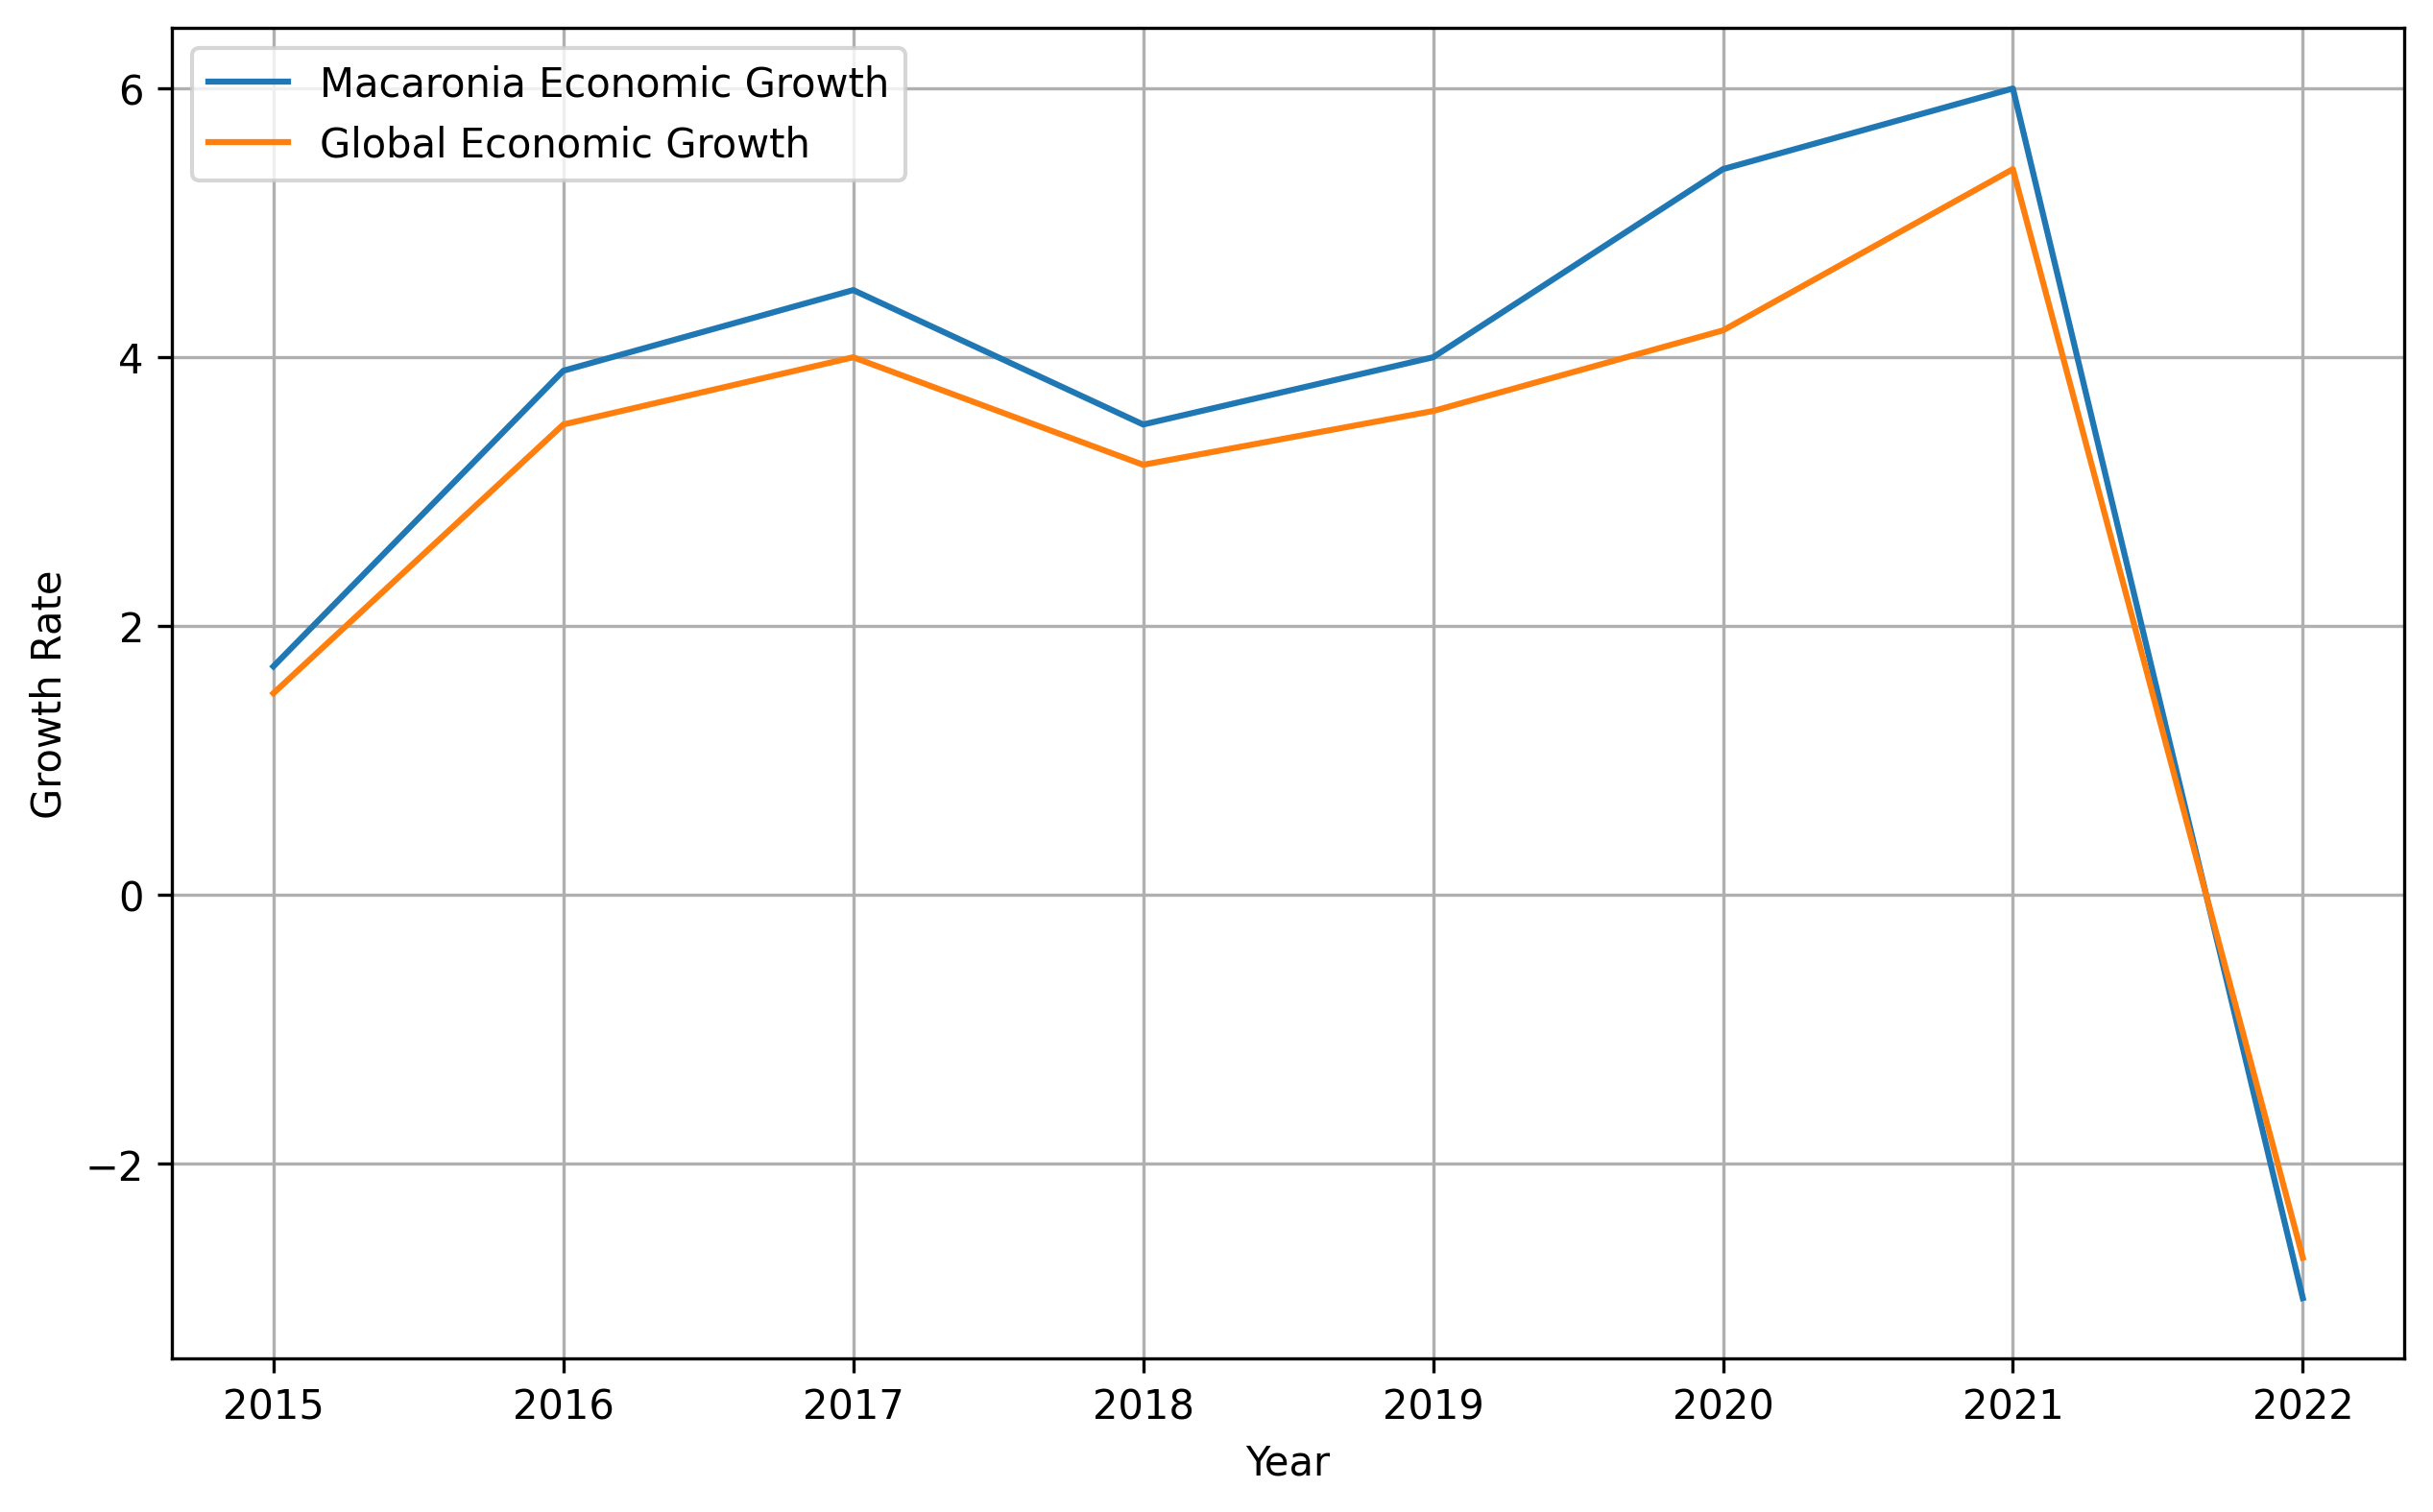
\includegraphics[width=0.5\textwidth]{growth.png}
     \caption{Macaronia Economic Growth vs Global Economic Growth}
     \label{fig:graph_1}
\end{figure}
\subsection*{The Perfect Storm}  

The collapse of a major U.S. financial institution and the ensuing turmoil in global credit markets have brought to light Macaronia's deep-seated vulnerabilities. 
This event sparked widespread uncertainty, prompting international investors to withdraw funds from emerging markets, including Macaronia. The nation’s stock market, cross-listed with U.S. exchanges,
experienced steep declines as capital fled, draining foreign reserves and weakening the national currency. With dwindling reserves, the central bank was unable to supply adequate emergency liquidity,
echoing the struggles seen in countries like \textbf{\textcolor{teal}{Argentina}} and \textbf{\textcolor{teal}{Greece}} during their financial crises.  \textcolor{orange}{\cite{IMF2023WEO}} % CITE: IMF2023WEO

This convergence of external shocks and internal frailties has pushed Macaronia’s financial system to the brink. \textbf{\textcolor{teal}{Undercapitalized banks}}, 
excessive exposure to \textbf{\textcolor{teal}{volatile REITs}}, and a lack of domestic financial resilience have created a fragile ecosystem, highly susceptible to global disruptions. 
The question is no longer if a crisis will occur, but when the next shock will tip the system into chaos. Amid rising global economic uncertainty, the countdown has begun, and the stakes are immense.  



\subsection*{Breakdown of Macaronia's Structural Vulnerabilities}  
Macaronia’s situation reflects a common challenge among Caribbean economies: \textbf{\textcolor{teal}{shallow domestic credit markets}} and limited financial depth.
These structural flaws make such economies highly prone to \textbf{\textcolor{teal}{external shocks}}. As global financial conditions tightened, the nation’s reliance on foreign liquidity 
shifted from a growth engine to a critical weakness. This sudden change laid bare the fragility of its financial system, already strained by undercapitalized banks, heavy investments in volatile REITs, 
and risky lending practices.  \textcolor{orange}{\cite{UNCTAD2023FDI}}



\subsection*{Breakdown of Global Economic Pressures}  
The first signs of trouble appeared as global interest rates rose and \textbf{\textcolor{teal}{credit conditions}} tightened. Higher borrowing costs made it harder for businesses and financial institutions to secure external financing, leading to a sharp drop in \textbf{\textcolor{teal}{foreign direct investment (FDI)}}. The 2007-2009 global financial crisis had already underscored the perils of overreliance on foreign capital. During that period, Macaronia, like other nations dependent on external funding, saw \textbf{\textcolor{teal}{capital flight}} as investors retreated from riskier markets.  

The recent failure of a major U.S. financial institution further destabilized global credit markets, intensifying Macaronia’s challenges. This event triggered a wave of uncertainty, prompting foreign investors to pull out of emerging markets, including Macaronia. The nation’s stock market, tied to U.S. exchanges, plummeted as capital fled, draining foreign reserves and weakening the currency. The central bank, already grappling with shrinking reserves, was unable to provide sufficient emergency liquidity, mirroring the struggles of countries like \textbf{\textcolor{teal}{Argentina}} and \textbf{\textcolor{teal}{Greece}} during their crises.  


\subsection*{Breakdown of Domestic Amplification of External Shocks}  
The global economic downturn, worsened by the U.S. financial institution’s collapse, had immediate and severe domestic consequences. \textbf{\textcolor{teal}{Inflation}}, previously stable, surged to \textbf{\textcolor{teal}{6.0\%}} in 2022, eroding purchasing power and straining household budgets. Simultaneously, \textbf{\textcolor{teal}{unemployment}} rose to \textbf{\textcolor{teal}{8.0\%}}, reflecting the broader economic contraction and fueling social tensions.  

These domestic pressures magnified the impact of external shocks, creating a vicious cycle. Rising inflation and joblessness reduced consumer spending, further weakening the economy. The interplay of global financial disruptions and internal economic distress pushed Macaronia’s financial system to the edge of collapse.  



\subsection*{Breakdown of Financial Sector Vulnerabilities}  
Macaronia’s financial sector, already burdened by heavy exposure to \textbf{\textcolor{teal}{Real Estate Investment Trusts (REITs)}}, faced heightened challenges as global credit markets tightened. Falling REIT values caused significant losses for banks and credit unions, many of which had heavily invested in these volatile assets. This triggered a \textbf{\textcolor{teal}{liquidity crunch}}, as institutions struggled to maintain adequate reserves and meet short-term obligations.  

The U.S. financial institution’s collapse served as a stark reminder of how declining asset values, particularly in real estate, can ignite widespread financial instability. In Macaronia, the effects were immediate: the stock market plunged, capital flight accelerated, and the currency came under intense pressure. With limited reserves, the central bank was unable to stabilize the situation, leaving the financial system dangerously exposed.  



\subsection*{Breakdown of Structural Weaknesses}  
Macaronia’s financial system was further crippled by deep-rooted structural flaws. High \textbf{\textcolor{teal}{collateral requirements}} and limited access to domestic credit, particularly for small and medium-sized enterprises, stifled economic growth and reinforced reliance on external financing. As global credit conditions tightened, this dependence became a critical liability.  

The absence of robust \textbf{\textcolor{teal}{macroprudential oversight}} also played a key role in the crisis. Unlike nations with strong systemic risk monitoring frameworks, such as those 
under the \textbf{\textcolor{teal}{European Systemic Risk Board}}, Macaronia lacked effective mechanisms to identify and address vulnerabilities. This left the country unprepared to manage the cascading failures 
triggered by global financial disruptions.  \textcolor{orange}{\cite{ECB2023ESRB}}



% 
\section{External Issues: Amplifyng the Crisis}

\subsection{ Collapse of a Major U.S. Financial Institution}


The Globalization of financial systems means that Macaronia’s economy is not immune to such external shocks. The moderate correlation between global economic growth and Macaronia’s economic growth (0.44) indicates that Macaronia's economy is somewhat exposed to global trends. Cross-listing of securities means that Macaronia's stock market is suffering from U.S. market volatility. The global credit crunch has limited foreign funding, worsening capital flight and currency depreciation, further destabilizing the economy.
For instance, the collapse has led to a tightening of global credit conditions, making it more difficult for Macaronia’s banks to access foreign funding. This has exacerbated liquidity shortages and increased borrowing costs, further straining the financial system.


\subsection{Global Economic Contractions}
Global economic contractions have further strained Macaronia's economy, although domestic factors remain the primary drivers of the crisis. While global trends affect Macaronia, as shown by the correlation between Macaronia's economic growth and global economic growth (0.44), domestic credit expansion has played a larger role in the current crisis. The correlation between credit union lending and economic growth (0.77) highlights that Macaronia's economic expansion has been debt-driven rather than export-driven. Slower global growth is dampening inflationary pressures, as indicated by the negative correlation between inflation and global growth (-0.46), but this provides little relief given the domestic challenges.
For example, the slowdown in global trade has reduced demand for Macaronia’s exports, further weakening the economy. This has been compounded by declining remittances from overseas workers, which have traditionally been a key source of foreign exchange.
\subsection{Capital Flight}

Capital flight has accelerated in response to the economic crisis, driven by concerns over currency depreciation and financial instability. The correlation between public debt to GDP and exchange rate (-0.68) confirms that capital flight is accelerating currency depreciation. Capital flight is also reducing financial stability, as shown by the correlation between liquidity ratios and exchange rate (-0.28), creating a vicious cycle of economic decline. Foreign investors are withdrawing from Macaronia's markets, further destabilizing the economy, as evidenced by the stock market decline and capital flight.
For instance, the withdrawal of foreign capital has led to a sharp decline in asset prices, particularly in the real estate and stock markets. This has further eroded investor confidence and increased the risk of a full-blown financial crisis.

\subsection{ Decline in Foreign Direct Investment (FDI)}
The decline in FDI is a significant concern, as it reflects eroding investor confidence in Macaronia's economic prospects. Investors fear further currency depreciation, which would erode returns on their investments, as indicated by the expected correlation between exchange rate and FDI (-0.68). Falling equity markets signal higher investment risks, discouraging FDI inflows. High public debt levels make Macaronia less attractive to foreign investors, as they perceive higher sovereign risk, as shown by the correlation between public debt to GDP and FDI (-0.45). The collapse of the real estate market, a key driver of FDI, has further reduced investor confidence.
For example, the cancellation of several major infrastructure projects due to funding shortages has sent a negative signal to foreign investors, further reducing FDI inflows.


% \section{Theoretical Frameworks and Analysis}

To gain a deeper understanding of Macaronia's economic crisis, we can apply several theoretical frameworks that elucidate the mechanisms amplifying financial instability.

\subsection{Financial Accelerator Theory}

The Financial Accelerator Theory, introduced by economists such as Ben Bernanke, Mark Gertler, and Simon Gilchrist, describes how financial market imperfections can amplify economic fluctuations. In essence, small economic shocks can be magnified through their impact on borrowers' balance sheets and the external finance premium—the cost difference between internal and external financing. For example, a decline in asset values reduces borrowers' net worth, increasing the external finance premium, which leads to reduced borrowing and investment, further suppressing economic activity. This cyclical process can exacerbate economic downturns.
federalreserve.gov

In Macaronia's context, the heavy reliance on the real estate sector has heightened this effect. As property values decline, borrowers' net worth diminishes, leading to higher borrowing costs and reduced access to credit. This contraction in lending further suppresses economic activity, creating a feedback loop that exacerbates the downturn. Such dynamics illustrate how initial shocks to asset values can be magnified through financial channels, deepening the economic crisis.

\subsection{Liquidity Transformation and Bank Vulnerability}

Liquidity transformation refers to the process by which banks fund long-term, illiquid assets with short-term, liquid liabilities, such as demand deposits. While this supports economic activity by providing liquidity to borrowers, it also exposes banks to liquidity risk. If many depositors withdraw their funds simultaneously—a scenario known as a bank run—banks may struggle to meet these demands due to the illiquidity of their assets. This fragility is inherent in the banking system's structure.

In Macaronia, banks' significant exposure to the volatile real estate market has intensified this risk. Declining real estate values impair banks' asset quality, making it challenging to meet short-term obligations and potentially leading to insolvency. This scenario underscores the fragility inherent in liquidity transformation, especially when asset markets experience significant downturns.

\subsection{Contagion Effects and Financial Globalization}

Financial contagion refers to the spread of market disturbances from one institution to others, leading to systemic crises. The collapse of a major U.S. financial institution has had ripple effects on Macaronia's financial system, highlighting the dangers of such contagion. Interconnectedness through cross-border investments and financial linkages means that shocks in one market can quickly transmit to others. This interconnectedness can lead to synchronized declines in asset values and increased volatility, further destabilizing economies like Macaronia's.

\subsection{Currency Instability and Exchange Rate Dynamics}

Currency instability can arise from various factors, including fiscal deficits, inflationary pressures, and capital flight. In Macaronia, persistent fiscal deficits and declining investor confidence have led to currency depreciation. This depreciation increases the cost of imports, fueling inflation and reducing purchasing power. The interplay between exchange rates and economic fundamentals can create a vicious cycle, where currency instability begets further economic challenges, complicating stabilization efforts.

\subsection{Deposit Insurance and Moral Hazard}

Deposit insurance is designed to protect depositors and maintain confidence in the banking system. However, it can also lead to moral hazard, where banks engage in riskier behavior, knowing that deposits are insured. In Macaronia, the presence of deposit insurance may have encouraged banks to undertake excessive risks, contributing to financial instability. This moral hazard underscores the need for careful design and regulation of deposit insurance schemes to balance depositor protection with prudent risk management.

% recommendations 
%\newpage 

\section*{Recommendations}

After the analysis, the government and the Central Bank should adopt a comprehensive strategy to 
stabilize the \textbf{\textcolor{teal}{financial sector}}, rebuild investor confidence, and promote 
long-term economic resilience in Macaronia. The following recommendations focus on enhancing
\textbf{\textcolor{teal}{monetary policy}}, strengthening financial stability, ensuring 
\textbf{\textcolor{teal}{exchange rate steadiness}}, and supporting vulnerable populations. 

\subsection*{Adjusting Monetary Policy to Help Balance Inflation \& Liquidity}

\begin{figure}[h]     
     \centering
     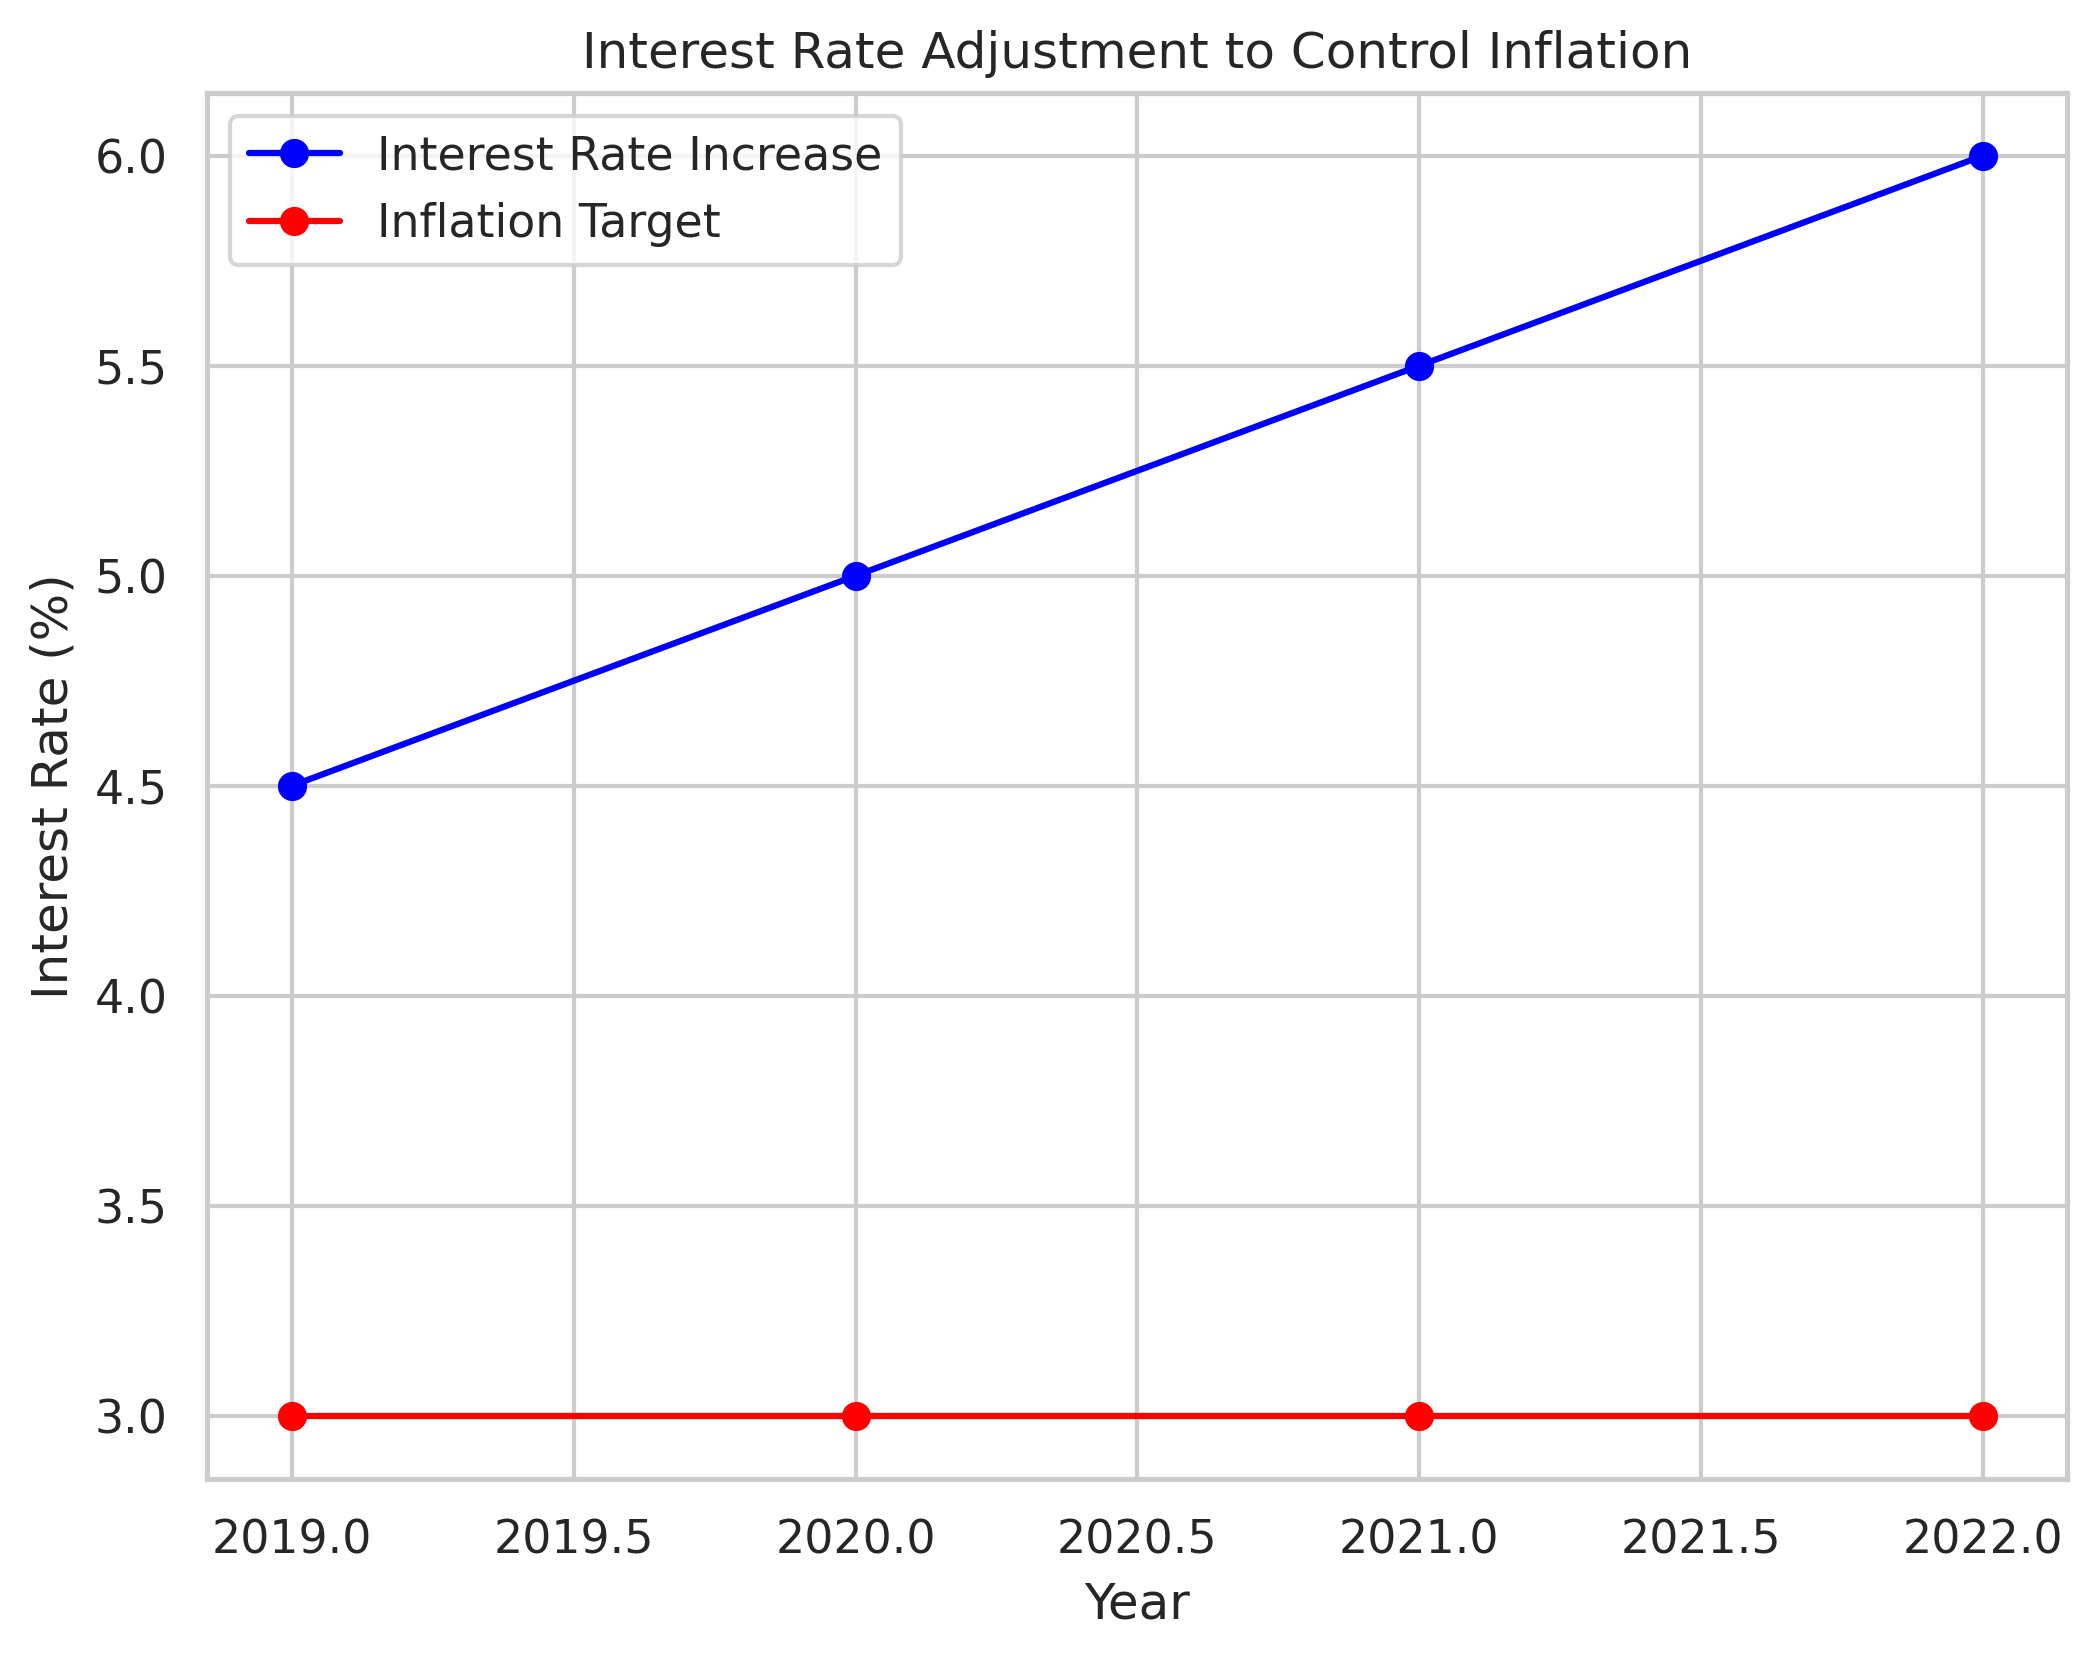
\includegraphics[width=0.53\textwidth]{adjustment.png}
     \caption{Interset Rate Ajustment to Control Inflation}
     \label{fig:graph_1}
\end{figure}

Monetary policy should aim to balance \textbf{\textcolor{teal}{inflation}} and liquidity. While raising \textbf{\textcolor{teal}{interest rates}} 
can help curb inflation, an overly aggressive approach may stifle economic activity and tighten credit conditions. A moderate increase from the current 
\textbf{\textcolor{teal}{4.5\%}} rate could ease inflationary pressures while preserving credit availability. 
Additionally, the Central Bank should introduce a \textbf{\textcolor{teal}{liquidity assistance program}} 
to provide short-term funding for institutions facing deposit outflows, ensuring stability without encouraging
excessive lending. 

Furthermore, targeted \textbf{\textcolor{teal}{open market operations (OMOs)}} should be 
employed to manage liquidity fluctuations. By selectively buying or selling bonds, the Central Bank can regulate
money supply and contain inflation without imposing unnecessary credit constraints \textcolor{orange}{\cite{claessens2017}}.
As shown in Figure 9, a moderate interest rate increase can help align the current rate with the inflation target, 
effectively controlling \textcolor{teal}{\textbf{inflationary pressures}}.

\newpage
\subsection*{Stabilizing the Exchange Rate and Strengthening Foreign Reserves}

\begin{figure}[h]     
     \centering
     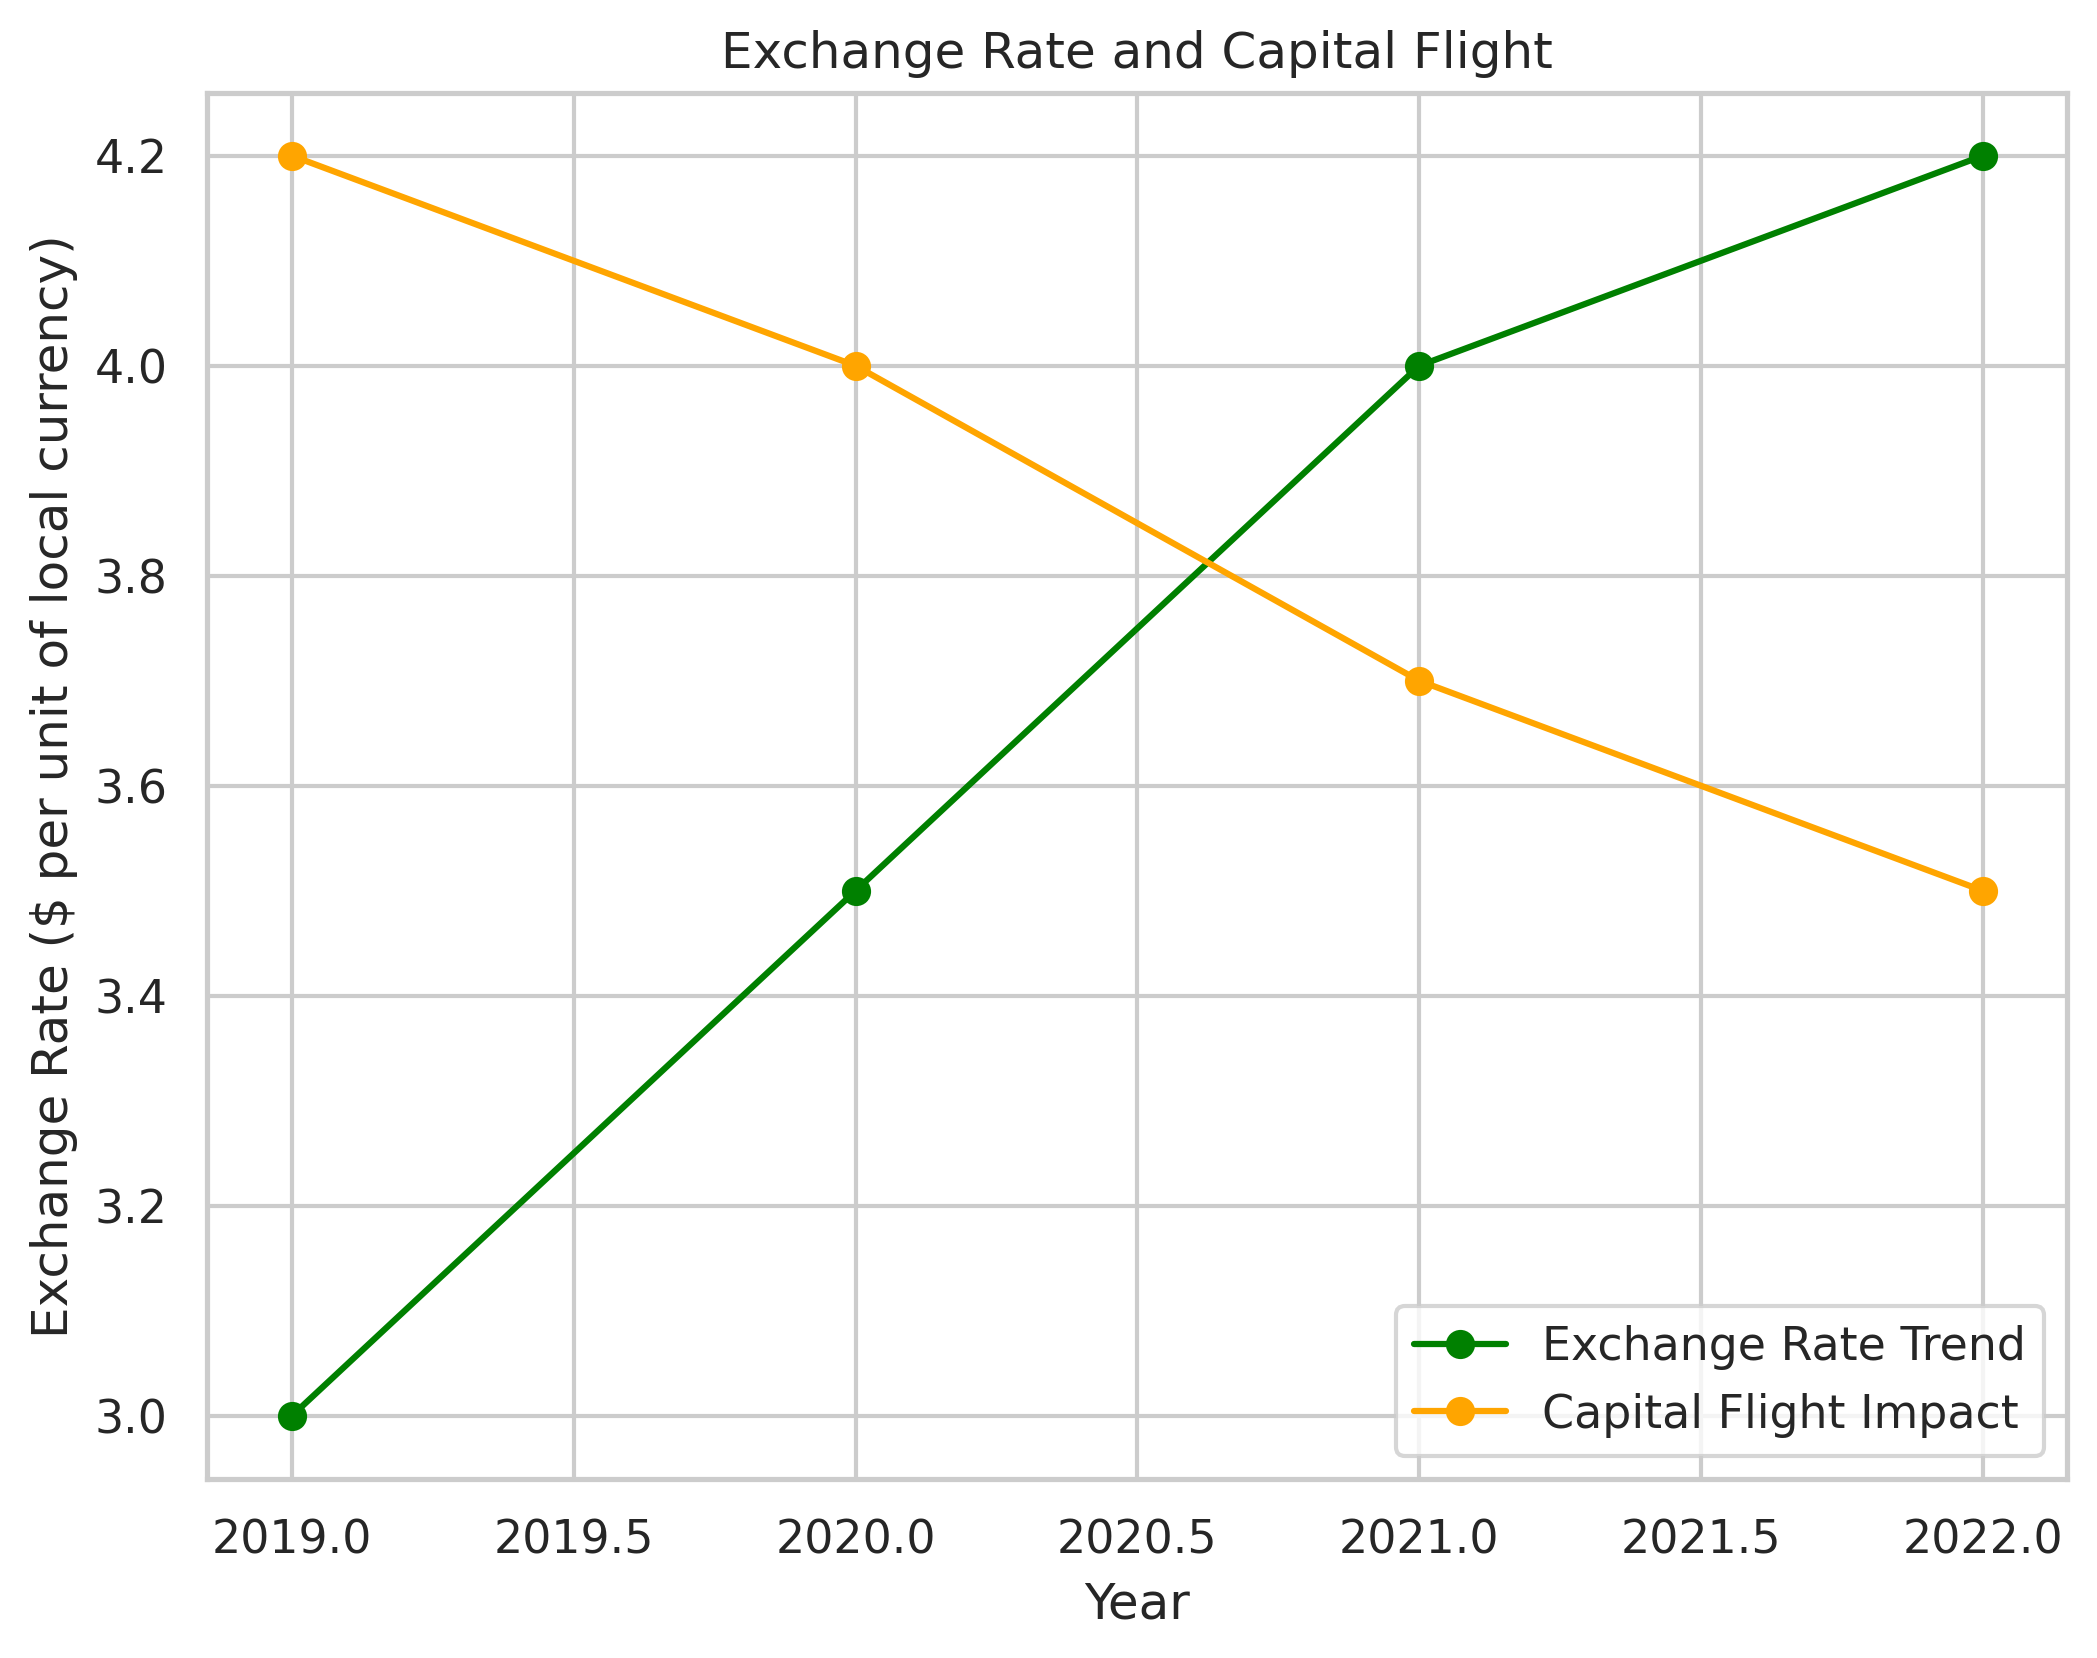
\includegraphics[width=0.53\textwidth]{exchange.png}
     \caption{Exchange Rate and Capital Flight}
     \label{fig:graph_1}
\end{figure}

As depicted in Figure 10, Macaronia's floating exchange rate is under significant
pressure due to \textcolor{teal}{\textbf{capital flight}} and investor withdrawals, 
leading to a rapid depletion of \textcolor{teal}{\textbf{international reserves}}. 
To counter this, the government should engage with the International Monetary Fund (IMF)
to secure a stabilization loan, ensuring that any assistance supports 
\textcolor{teal}{\textbf{long-term economic stability}} rather than providing only short-term 
liquidity relief. Additionally, to rebuild investor confidence, the government should implement 
measured \textcolor{teal}{\textbf{capital controls}} that deter speculative currency outflows while
preserving flexibility for legitimate trade and investment \textcolor{orange}{\cite{imf2024}}.



\subsection*{Strengthening Financial Sector Stability}
Macaronia’s financial sector, particularly commercial banks and credit unions, 
is highly exposed to the \textbf{\textcolor{teal}{real estate market}}, with 
\textbf{\textcolor{teal}{15\%}} and \textbf{\textcolor{teal}{20\%}} of their assets linked to 
\textbf{\textcolor{teal}{Real Estate Investment Trusts (REITs)}}. This concentration has heightened 
systemic risks, especially as REIT values have declined. To mitigate these vulnerabilities, 
the Central Bank should enforce stricter \textbf{\textcolor{teal}{capital adequacy ratios}},
requiring financial institutions to allocate more assets to lower-risk investments
\textcolor{orange}{\cite{mishkin2021}}.


A phased \textbf{\textcolor{teal}{recapitalization process}} should support weaker banks,
incorporating private capital injections, foreign financial assistance, and government-backed stabilization
funds. Furthermore, banks and credit unions should be encouraged to diversify their asset portfolios by
investing in more stable sectors such as \textbf{\textcolor{teal}{manufacturing}},
\textbf{\textcolor{teal}{technology}}, and \textbf{\textcolor{teal}{renewable energy}}. 
Strengthening financial regulations is essential to prevent future crises,
including the creation of an independent financial stability oversight council to monitor systemic risks.
Enhanced transparency and disclosure requirements would further bolster market confidence in financial 
institution \textcolor{orange}{\cite{reinhart2009}}.

\subsection*{Restoring Investor and Depositor Confidence}

\begin{figure}[h]     
     \centering
     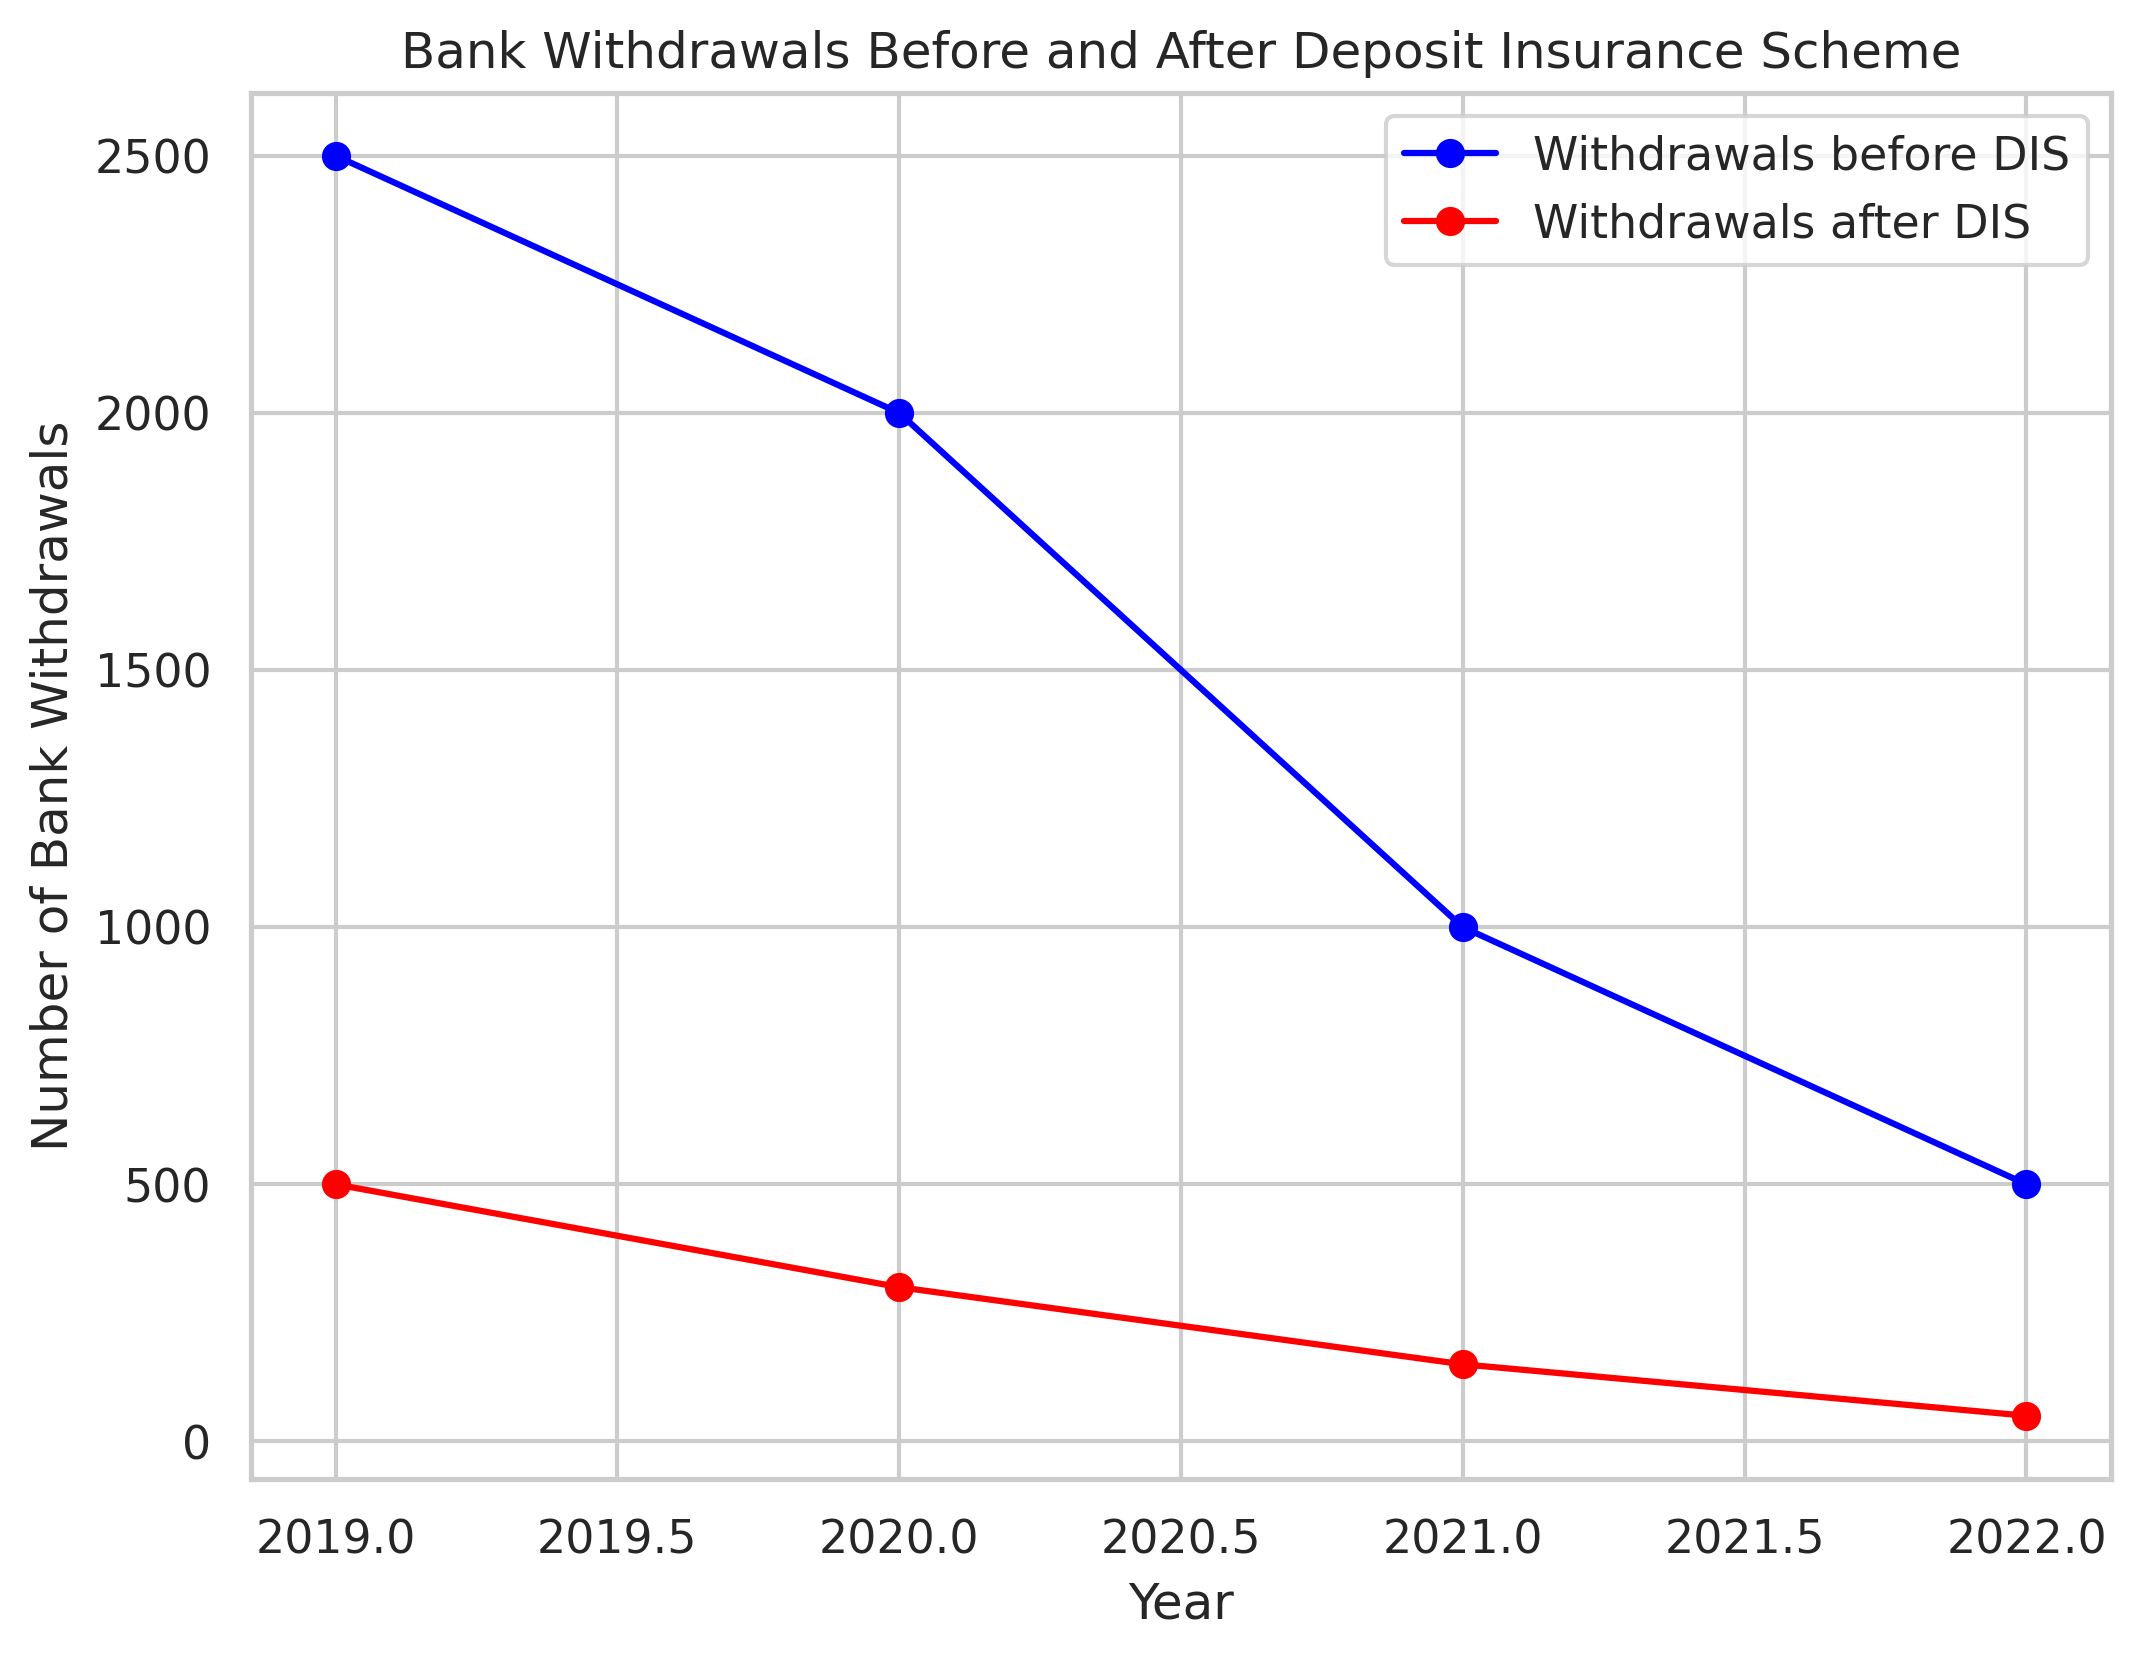
\includegraphics[width=0.53\textwidth]{restore.png}
     \caption{Bank Witdrawals Before And After Deposit Insurance Scheme}
     \label{fig:graph_1}
\end{figure}

Macaronia faces a growing crisis of \textcolor{teal}{\textbf{depositor confidence}}, leading 
to increasing bank withdrawals, a trend evident in Figure 11. The recent collapse of two commercial
banks due to poor capitalization has intensified concerns over \textcolor{teal}{\textbf{financial stability}}.
To address this, the government should introduce a \textcolor{teal}{\textbf{Deposit Insurance Scheme (DIS)}},
which, as Figure 11 suggests, would protect deposits up to a set limit, reducing panic-driven bank runs and 
reassuring depositors of their funds' security. \textcolor{teal}{\textbf{Restoring investor confidence}} is
essential for revitalizing capital inflows into the economy.

To enhance financial transparency,the Central Bank and regulatory authorities 
should regularly publish financial stability reports outlining the state of the
banking sector and ongoing stabilization measures. Additionally, the government
should use tax incentives, investment guarantees, and low-interest loans to attract 
long-term investors. Strengthening investor protection laws and corporate governance will 
further assure both foreign and domestic investors of asset security \textcolor{orange}{\cite{gorton2012}}.

\subsection*{Supporting Financially Excluded and Repressed Households}

The economic downturn has disproportionately affected lower-income households, vulnerable groups, 
and small businesses in Macaronia, limiting access to credit, employment, and essential services.
To mitigate these impacts, the government, should implement targeted 
\textcolor{teal}{\textbf{social protection programs}}, including direct cash transfers to low-income 
households to ensure basic needs are met, subsidized credit programs to support small and medium-sized
businesses, and temporary rent and mortgage relief to prevent widespread foreclosures and homelessness
amid the real estate downturn. As illustrated in Figure 12, a significant portion of the targeted social 
protection programs should be allocated to \textcolor{teal}{\textbf{low-income households}}
(\textcolor{teal}{\textbf{40.0\%}}), followed by \textcolor{teal}{\textbf{financially vulnerable groups}} 
(\textcolor{teal}{\textbf{30.0\%}}) and \textcolor{teal}{\textbf{small businesses}}
(\textcolor{teal}{\textbf{30.0\%}}).


\begin{figure}[h]     
     \centering
     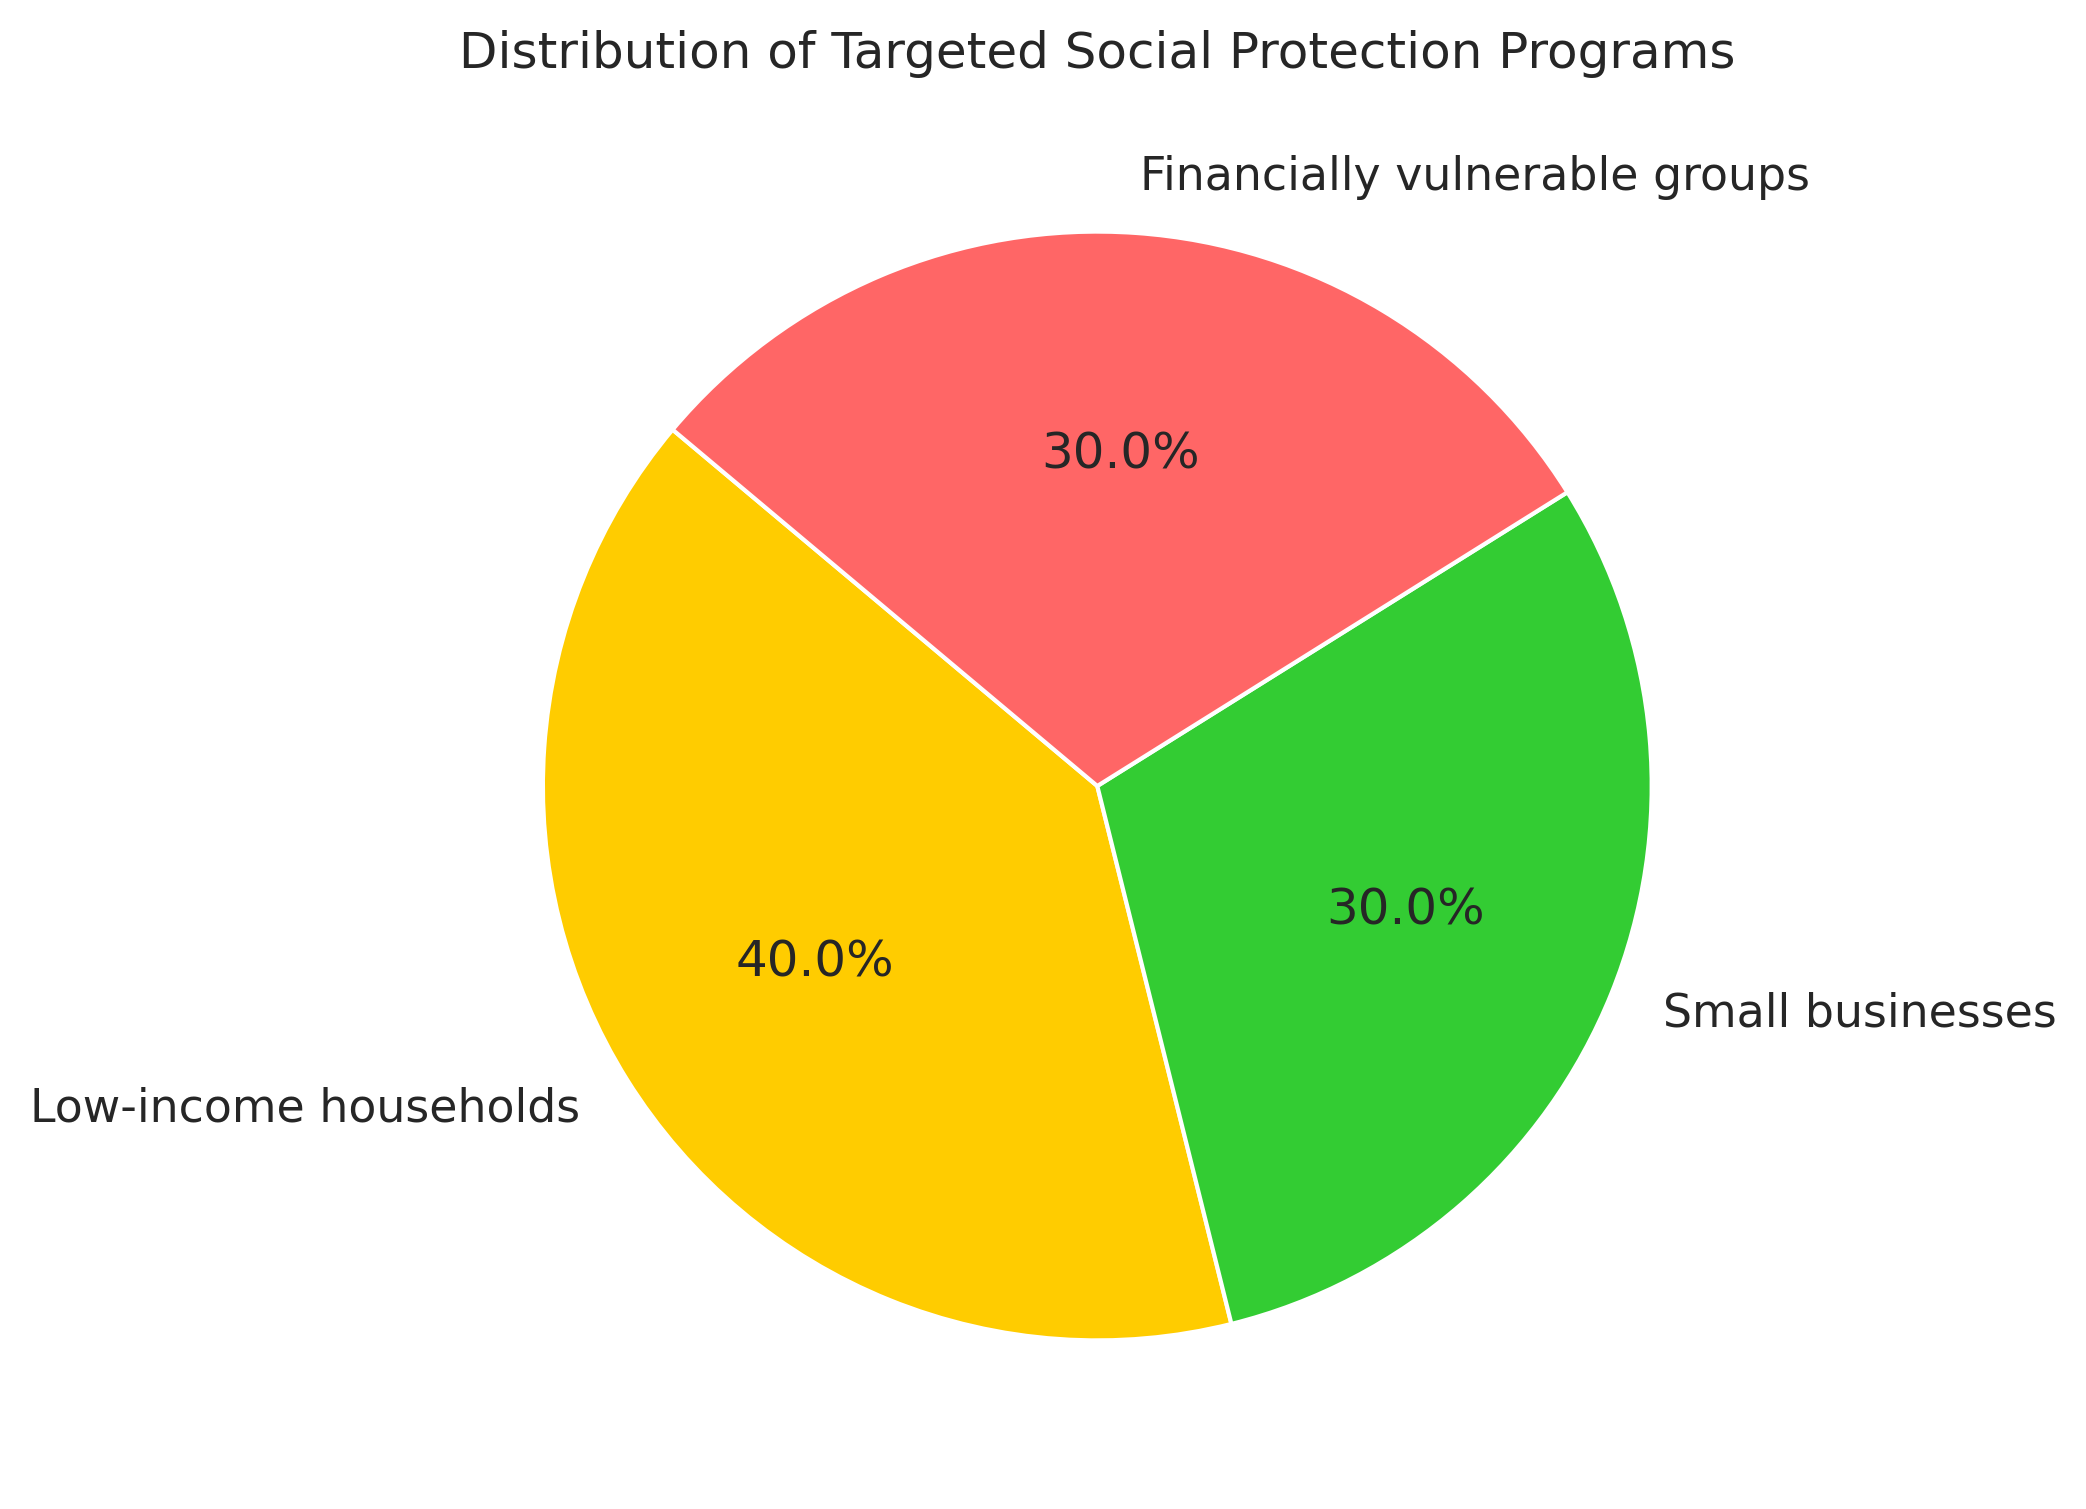
\includegraphics[width=0.53\textwidth]{support.png}
     \caption{Distribution of Targeted Social Platforms}
     \label{fig:graph_1}
\end{figure}

Expanding financial inclusion initiatives will further ensure that 
at-risk populations have access to affordable financial services. Strengthening the 
role of credit unions and microfinance institutions in providing low-interest loans to 
small businesses and individuals will promote economic resilience and stability \textcolor{orange}{\cite{worldbank2023}}.

\subsection*{Promoting Economic Diversification and Long-Term Growth}

\begin{figure}[h]     
     \centering
     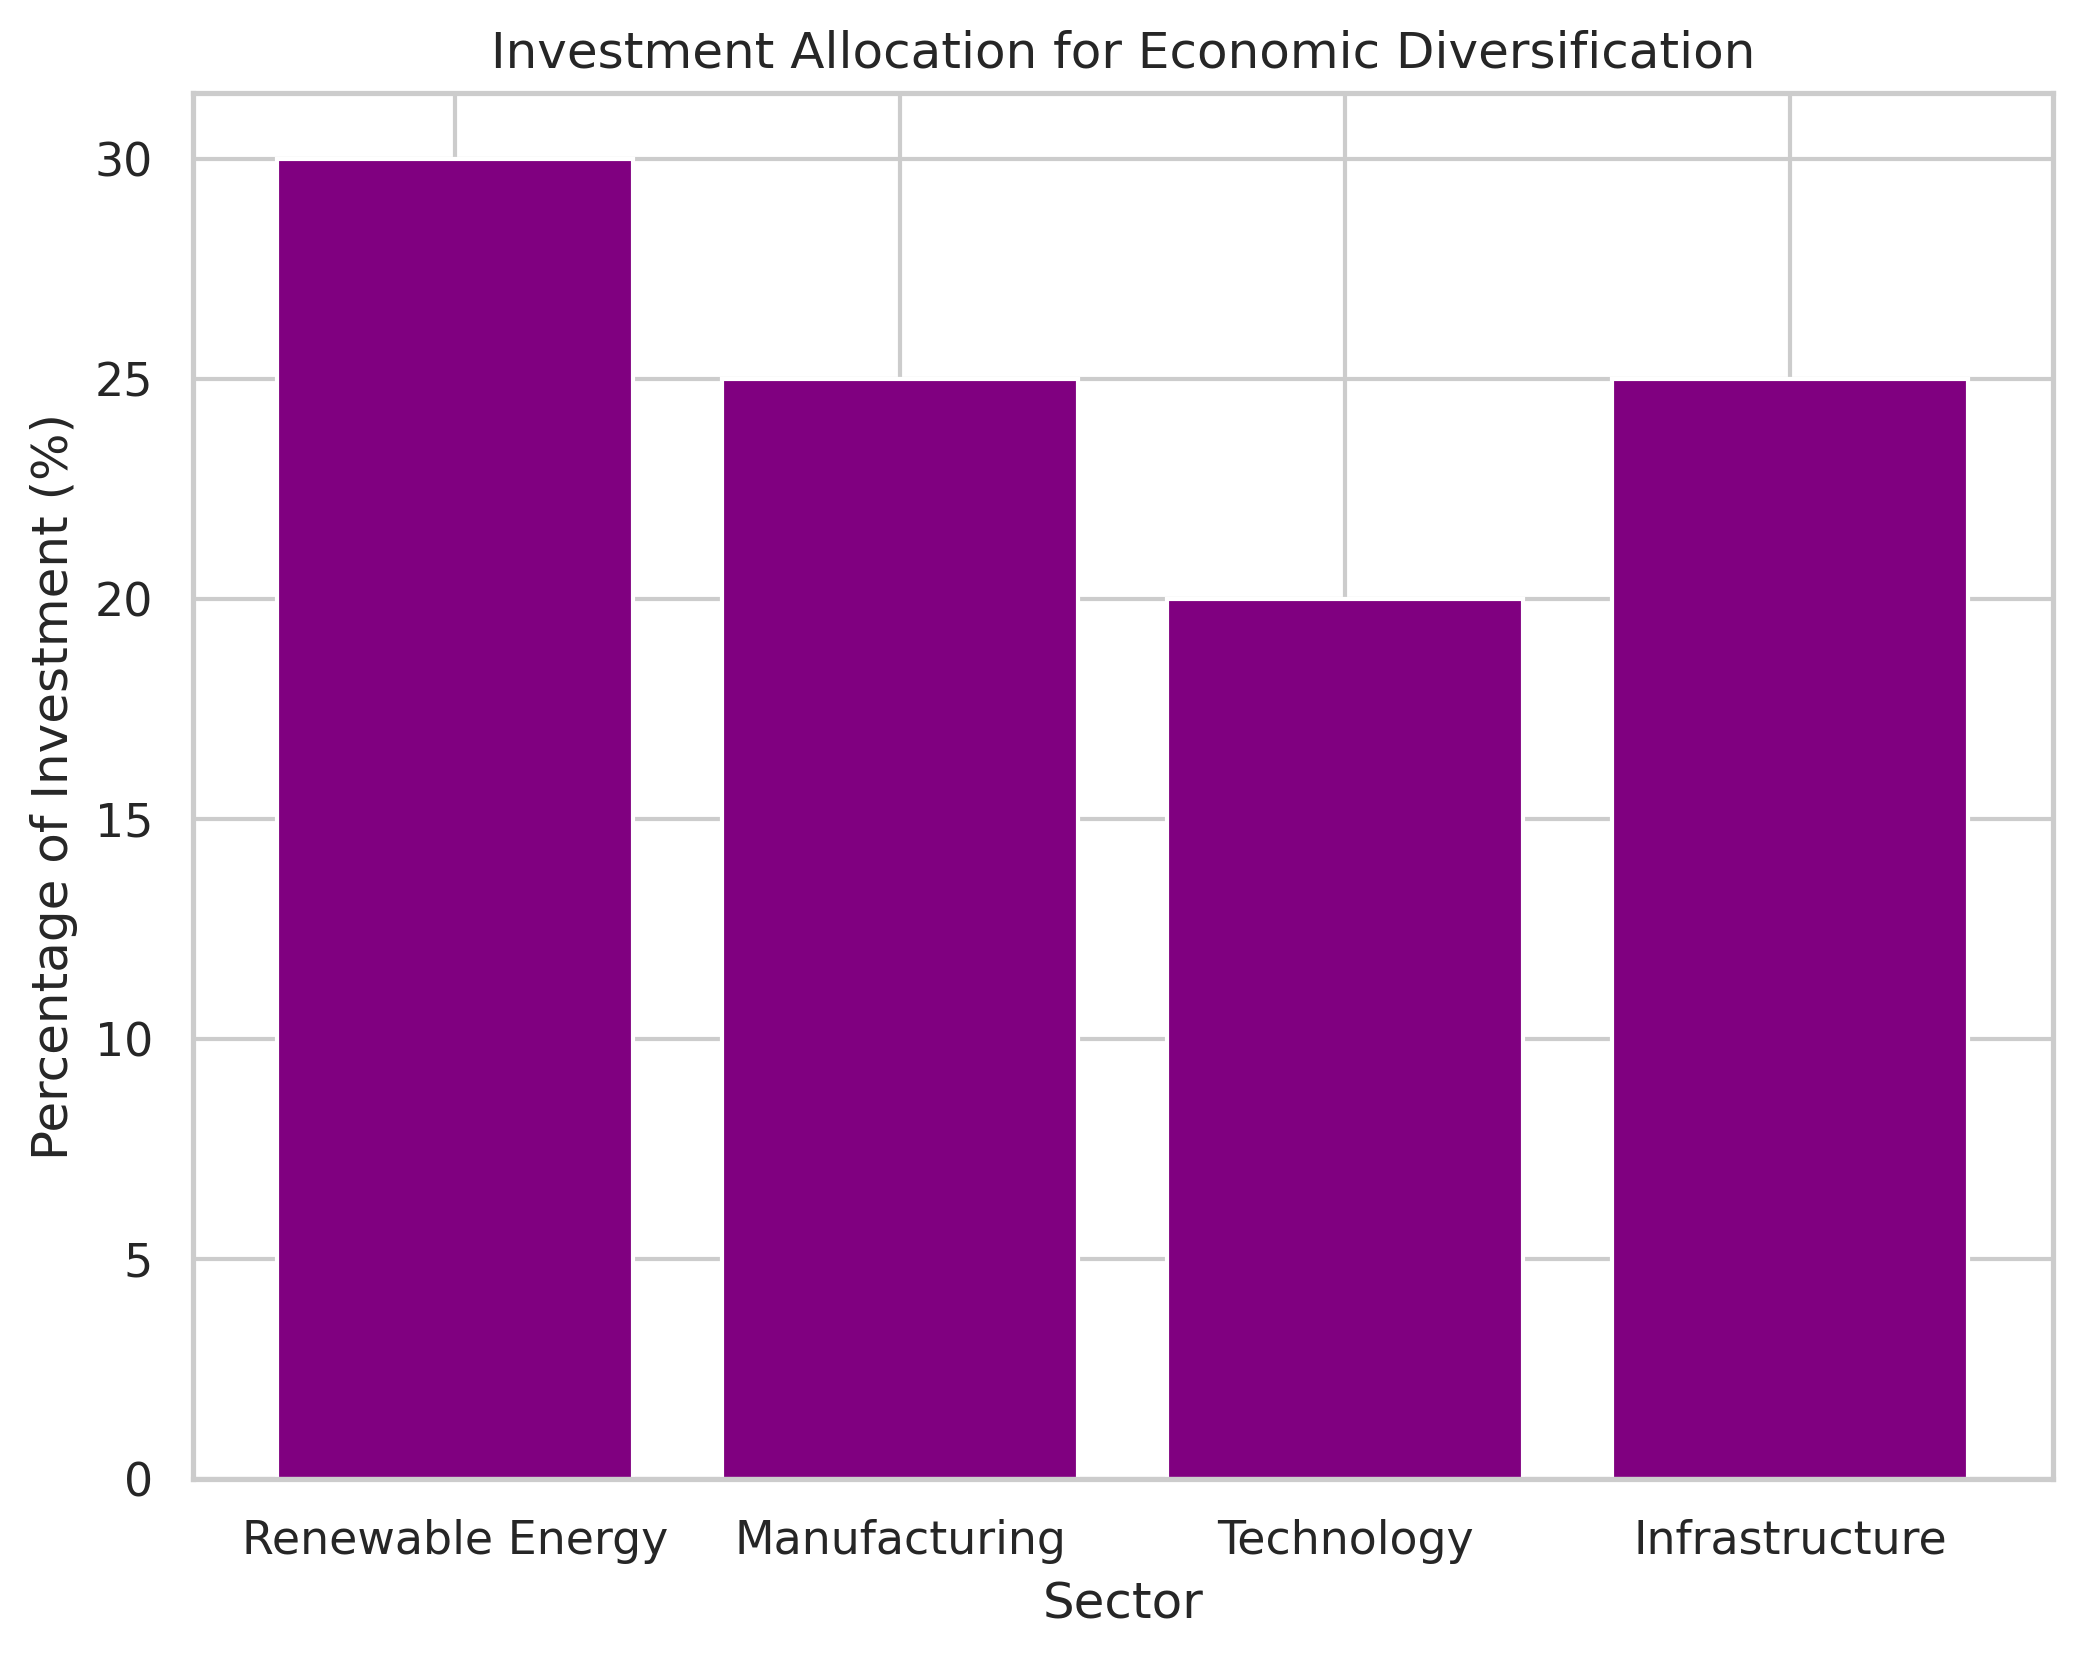
\includegraphics[width=0.53\textwidth]{diversification.png}
     \caption{Investment Allocation for Economic Diversification}
     \label{fig:graph_1}
\end{figure}


Macaronia's economic expansion has been overly reliant on a booming
\textcolor{teal}{\textbf{real estate market}}, which has proven unsustainable.
\textcolor{teal}{\textbf{Diversification}} is essential, and the government should
prioritize domestic economic growth through targeted infrastructure and industrial 
expansion. A key strategy to achieve this is through
\textcolor{teal}{\textbf{Public-Private Partnerships (PPPs)}}, enabling 
collaboration between the private sector and government to develop and manage public
infrastructure. To address logistical bottlenecks and enhance business efficiency, investments
should focus on \textcolor{teal}{\textbf{energy}}, \textcolor{teal}{\textbf{transportation}},
and \textcolor{teal}{\textbf{digital infrastructure}}. As shown in Figure 13, the recommended
investment allocation for economic diversification includes 
\textcolor{teal}{\textbf{Renewable Energy}} (\textcolor{teal}{\textbf{30\%}}),
\textcolor{teal}{\textbf{Manufacturing}} (\textcolor{teal}{\textbf{25\%}}), 
\textcolor{teal}{\textbf{Technology}} (\textcolor{teal}{\textbf{20\%}}), and 
\textcolor{teal}{\textbf{Infrastructure}} (\textcolor{teal}{\textbf{25\%}}). 
Expanding renewable energy, modernizing ports, and improving road networks will boost
competitiveness, attract long-term investment, and reduce import dependency \textcolor{orange}{\cite{engel2014}}.

Given Macaronia's high \textcolor{teal}{\textbf{public debt}} of \textcolor{teal}{\textbf{80\% of GDP}},
direct government-funded projects are financially unfeasible. Utilizing PPPs will allow critical investments
without further straining fiscal deficits. Structuring agreements with risk-sharing mechanisms will ensure 
financial risks are distributed between public and private entities rather than burdening the government alone.
Additionally, infrastructure projects and industrial investments can drive 
\textcolor{teal}{\textbf{job creation}} and \textcolor{teal}{\textbf{economic inclusion}}, 
particularly for low-income and financially marginalized populations. Encouraging private sector
participation in vocational training programs will help develop a skilled workforce to support
diversified economic growth. Strengthening public-private partnerships will ensure that economic
expansion is not overly reliant on foreign capital inflows \textcolor{orange}{\cite{bernanke2013}}.

% Conclusion
%\section*{Conclusion}

Macaronia’s economic disaster stems from both internal financial susceptibilities and external shocks. The disproportionate reliance on \textbf{\textcolor{teal}{real estate investments}}, weak financial inaccuracy, and aggressive \textbf{\textcolor{teal}{lending practices}} have considerably debilitated the economy, making the economy highly susceptible to global financial turmoil. Coupled with the breakdown of one of their major U.S. financial institutions and the intensifying \textbf{\textcolor{teal}{public sector debt}} and investor withdrawals, the economy has been pushed to the brink of a \textbf{\textcolor{teal}{financial meltdown}}.  

A comprehensive intervention strategy is needed to navigate out of this crisis; Macaronia must implement a set of reforms that highlight \textbf{\textcolor{teal}{investor confidence}}, \textbf{\textcolor{teal}{financial stability}}, and \textbf{\textcolor{teal}{economic diversification}}. Adjusting \textbf{\textcolor{teal}{monetary policy}} through restrained \textbf{\textcolor{teal}{interest rate upsurges}} and targeted \textbf{\textcolor{teal}{liquidity support}} will help maintain inflation without stifling economic activity. Securing \textbf{\textcolor{teal}{IMF}} assistance and employing strategic \textbf{\textcolor{teal}{exchange rate management}} measures will immensely help restore currency stability and rebuild foreign reserves. 

Strengthening \textbf{\textcolor{teal}{financial regulations}} and lowering the country’s banks’ overreliance on real estate investment will enable the long-term stability of the \textbf{\textcolor{teal}{financial sector}}. Announcing a \textbf{\textcolor{teal}{deposit insurance structure}} and communicating concise recovery measures will help restore depositor and investor confidence. Along with \textbf{\textcolor{teal}{social protection programs}} and \textbf{\textcolor{teal}{financial inclusion initiatives}} being employed, vulnerable households and small businesses will feel supported, thus ensuring that economic recovery curricula benefit all segments of society. 

Ultimately, Macaronia must embrace \textbf{\textcolor{teal}{economic diversification}} to have a decline in its dependence on volatile asset markets. With the promotion of \textbf{\textcolor{teal}{infrastructure development}} for economic resilience, reduction of the government’s fiscal burden, and the enhancement of \textbf{\textcolor{teal}{job creation}} and \textbf{\textcolor{teal}{economic inclusion}}, a structural economic strategy is employed that not only stabilizes the economy but also advocates for long-term sustained growth beyond fiscal sector reforms. To conclude, the path to the country’s recovery will require long-term commitment, decisive action, and cooperation between the government, financial institutions, and international partners. This will all be essential to successfully navigating and managing the crisis and fortifying long-term prosperity.

%\nocite{*}
%\printbibliography % Generates the references section

% EXAM NOTES %
%------------%
\tableofcontents

\newpage

\lecturetitle{1}{Introduction to Financial Systems}


\section{The Global Financial System}

The global financial system is a complex network of financial institutions, markets, instruments, and regulations that operate internationally to facilitate the allocation of capital, risk-sharing, and financial services across borders. This system encompasses banks, capital markets, insurers, central banks, and international financial institutions, as well as regulatory frameworks that govern cross-border financial activities.

\section{The Financial System}

The financial system is complex, and comprises different types of private sector financial institutions. Financial Markets channel funds from households, firms, and governments to those who may have a shortage of funds. They do this through financial intermediaries and financial markets. Key institutions include:
\begin{itemize}
    \item Banks
    \item Credit Unions
    \item Insurance Companies
    \item Mutual Funds
    \item Pension Funds
    \item Finance Companies
\end{itemize}

\section{The Financial Systems of CARICOM}

The financial sector within CARICOM is predominantly bank-centric with other important sectors such as credit unions, insurance companies and pension funds. The banking sectors in the region are a mix of local and foreign-owned entities (usually subsidiaries of Canadian parent companies).

\section{The Function of Financial Markets}

\subsection{Direct Finance}
\begin{itemize}
    \item Borrowers borrow funds directly from lenders in financial markets by selling them securities/financial instruments (which are claims on the borrower’s future income or assets).
    \item \textbf{Why is this important?}
    \begin{itemize}
        \item Persons who save are not the same as the ones who may profit from investment opportunities.
        \item In the absence of financial markets, lenders and borrowers are unlikely to meet/connect.
    \end{itemize}
\end{itemize}
\textit{The principal lender-savers are households, while governments, businesses, and foreigners may also have additional funds to lend out. On the other hand, the most important borrower-spenders are businesses and the government.}

\subsection{Indirect Finance}
\begin{itemize}
    \item The Financial Intermediary (FI) borrows funds from lenders-savers and then makes loans to borrowers/spenders.
    \item This process is called \textbf{financial intermediation} and is the primary route for moving funds between lenders and borrowers.
    \item In considering indirect finance, we must also consider transaction costs, risk sharing, and information costs in financial markets.
\end{itemize}
\textit{Funds may also move from lenders to borrowers through indirect finance – because it relies on a financial intermediary (FI) to facilitate the transaction.}

\section{The Structure of Financial Markets}

\subsection{Debt and Equity Markets}
A firm or individual may obtain funds in a financial market in two ways. The most common method is to issue a \textbf{debt instrument}, such as a bond or a mortgage. The maturity of a debt instrument is number of years (term) until that instrument’s expiration date. Alternatively, they can issue \textbf{equity}, such as common stock, which are claims to share in the net income and assets of a business.

\subsection{Primary and Secondary Markets}
\begin{itemize}
    \item A \textbf{primary market} is a financial market in which new issues of a security, such as a bond or a stock, are sold to initial buyers by the cooperation or government agency borrowing funds.
    \item A \textbf{secondary market} is a financial market in which securities which have been previously issued can be resold.
\end{itemize}

\subsection{Exchanges and Over-the-Counter Markets}
\textit{Secondary markets are organized in two ways:}
\begin{itemize}
    \item \textbf{Exchanges} are where buyers and sellers of securities (or their agents or brokers) meet in one central location to conduct trades, e.g. NYSE, FTSE, Chicago Board of Trade (CBOT).
    \item \textbf{Over-the-Counter (OTC) Markets} are markets in which dealers at different locations have an inventory of securities which they make available for trade (available to be bought and sold).
\end{itemize}

\subsection{Money and Capital Markets}
\begin{itemize}
    \item The \textbf{money market} is a financial market in which only short-term debt instruments (generally with a maturity less than one year) are traded.
    \item The \textbf{capital market} is the market in which longer-term debt (generally with original maturity of one year or greater) and equity instruments are traded.
\end{itemize}

\section{Transaction Costs}

\textit{Transaction costs relate to the time and money spent in carrying out financial transactions.}

\subsection{Transaction costs and Financial Intermediaries}
\begin{itemize}
    \item Financial intermediaries reduce transaction costs because they have developed the expertise and scale to be able to lower them.
    \item This ability to reduce transaction costs allows FIs to be able to provide funds to households and businesses with productive investment opportunities.
    \item Additionally, with low transaction costs, FIs can provide its customers with liquidity services to allow customers to conduct transactions.
\end{itemize}

\section{Risk Sharing}

\textit{An additional benefit of low transaction costs of FIs is that they can help reduce exposure of investors to risk, i.e. uncertainty regarding the returns to assets.}

\subsection{Risk Sharing and Financial Intermediaries}
\begin{itemize}
    \item Financial intermediaries reduce risk through a process known as \textbf{risk sharing}.
    \item FIs create assets with risk characteristics that people are comfortable with, and use this revenue to acquire more risky assets with higher return profiles. This process of risk sharing is also known as \textbf{asset transformation}.
    \item FIs also promote risk sharing by helping individuals to diversify their portfolios.
\end{itemize}

\section{Information Costs / Asymmetric Information}

\textit{In financial markets, one party often does not know enough about the other party to make accurate decisions. This is known as \textbf{asymmetric information}.}

\subsection{Asymmetric Information and Financial Intermediaries}
\begin{itemize}
    \item \textbf{Adverse selection} is the problem created by asymmetric information \emph{before} the transaction occurs. This happens when potential borrowers who may produce a poor (adverse) outcome are the ones who actively seek out loans. Because adverse selection makes it more likely that loans might be made to bad credit risks, lenders may decide not to make any loans even though there are good credit risks in the marketplace.
    \item \textbf{Moral hazard} is the problem created by asymmetric information \emph{after} the transaction occurs. Moral hazard is the risk (hazard) that the borrower might engage in activities that are undesirable (immoral) from the lender’s point of view, because they make it less likely that the loan will be paid back. Because moral hazard lowers the probability that the loan will be repaid, lenders may decide that they would rather not make a loan.
    \item Financial intermediaries can reduce problems arising from asymmetric information by screening potential borrowers (reducing adverse selection) and monitoring borrowers' activities (reducing moral hazard).
\end{itemize}

\section{Financial Market Infrastructure (FMI)}

Supporting the activities of financial markets and financial intermediaries are financial market infrastructures (FMIs). These are primarily payment and settlement system institutions such as real-time gross settlement systems (RTGS), automated clearing houses (ACH) and exchanges.

\subsection{The Caribbean’s Financial Market Infrastructure}
Financial market infrastructures are at varying levels of development across the region. Credit bureau development has been relatively slow.

\section{Types of Financial Institutions}

Financial intermediaries fall into three (3) categories:
\begin{enumerate}
    \item Depository institutions (Banks)
    \item Contractual savings institutions, and
    \item Investment Intermediaries.
\end{enumerate}
These are alternatively termed: (1) Banks, (2) Near-bank financial institutions, and (3) Non-Bank Financial institutions. Examples of these institutions include:
\begin{itemize}
    \item Commercial banks
    \item Savings and loans associations
    \item Credit unions
    \item Insurance companies
    \item Pension funds
    \item Mutual funds
    \item Money market mutual funds
\end{itemize}

\section{Regulation of Financial Institutions}

The financial system remains one of the most heavily regulated sectors in most economies. The government regulates the financial markets and institutions for two (2) main reasons:
\begin{enumerate}
    \item To increase the information available to investors, and
    \item Ensure the soundness of the financial system and by extension the institutions.
\end{enumerate}
Key regulatory concepts and frameworks include:
\begin{itemize}
    \item Basel Committee on Bank Supervision standards (e.g., Basel III)
    \item Solvency I and II (for insurance companies)
    \item PEARLS (for credit unions)
\end{itemize}

\subsection{Micro-prudential Regulation and Supervision}
\begin{itemize}
    \item \textbf{Micro-prudential regulation:} public regulations that aim at maintaining stability of individual institutions.
    \item \textbf{Micro-prudential supervision:} Oversight of specific intermediaries or markets. Examines the responses of an individual intermediary (banks, credit unions, insurance companies, pension funds) or market to exogenous shocks. Neglects the systemic implications of common behavior.
    \item Focuses on individual institutions.
\end{itemize}

\subsection{Macro-prudential Regulation and Supervision}
\begin{itemize}
    \item \textbf{Macro-prudential regulation:} public regulations that aim at maintaining systemic stability.
    \item \textbf{Macro-prudential supervision:} Public oversight that aims at identifying and containing systemic risks. Identification and assessment of risks and vulnerabilities in a whole financial system.
    \item Focuses on systemic risk.
\end{itemize}

\newpage

\section{Problem Set 1}

\begin{enumerate}

    \item Define \textbf{financial systems}. What are their primary components, and why are
    they significant in the economy?
       \begin{itemize}
           \item Financial systems are a network of instruments, institutions, markets and regulation that facilitate the flow of funds within the economy. It comprises of banks, near-bank institutions(such as credit unions), non-bank financial institutions (such as insurance companines), etc. These systems are detrimental because 
                 they efficently help allocate resources efficently by channelling funds from savers (those who have surplus funds) to borrowers (those in need of funds). For example, households may need financing for big purchases like cars or houses, while businesses may seek capital to expand their operations through investments in
                 infrastructure or equipment. 
       \end{itemize}

    \item What is the difference between \textbf{direct and indirect finance}? Provide examples
    of each.
      \begin{itemize}
          \item Direct finance occurs when borrower obtain funds directly from lenders without the use of financial intermediaries. This typically occurs through financial markets, such as when instruments (corporation bonds or stocks) are bought by investors. Indirect finance, on the other hand involves financial intermediation-such as banks 
                or credit unions who channel funds from savers to borrowers. For instance, when an individual deposits money into a bank, the bank may lend a portion of those funds to businesses or households, effectively transfering funds indirectly.
      \end{itemize}
    \item Explain the importance of \textbf{financial intermediaries} in reducing transaction
    costs and risks.
      \begin{itemize}
          \item Minimum efficent scale is larger for businesses than most individuals can invest. Someone with \$100, \$1000, \$1000, \$10,000 or even \$100,000 to invest would 
                have a hard time turning over a profit. This in because most of their profits would be eaten up by transaction costs like banking and broker fees, dealer spreads, attorney 
                fees, liquidity and diversification losses and the opportunity cost of his or her time. Financial intermediaries on the other hand are specialized to deal with transaction costs due to economics of scale 
                and risk sharing. By pooling together funds from many investors, they also enable diversification and risk-sharing, making investments more efficient and less risky for individual particpants.  
      \end{itemize}

    \item Discuss the function of \textbf{financial markets}. How do they facilitate the connection
    between savers and borrowers?
       \begin{itemize}
           \item Financial markets serve the primary function of channeling funds from savers to those who need it for either consumption or investment purchases. Savers provide funds by purchasing financial instruments 
                 such as bonds, stocks or deposits. These instruments represent a financial claim or future income. Borrowers such as businesses or governments seeking funding for public projects-issue these instruments to raise capital. 
       \end{itemize}

    \item Differentiate between \textbf{primary and secondary markets}. How do they contribute
    to the overall financial system?

    \item Explain the key differences between \textbf{debt markets and equity markets}.

    \item Describe the structure of the \textbf{Caribbean financial system}. What are the
    primary institutions involved?

    \item Discuss the \textbf{challenges facing the development} of financial market
    infrastructure in the Caribbean.

    \item Why is the \textbf{financial sector heavily regulated}? Outline the two main reasons for
    regulation.

    \item Explain how \textbf{financial intermediaries manage risks} through risk sharing and
    asset transformation.

\end{enumerate}

\newpage

\lecturetitle{2}{Theories of Financial Intermediation}


\subsection*{What is a Financial Intermediary?}

\begin{itemize}
    \item ``An Economic agent which specializes in the activities of buying and selling (usually at the same time) financial claims.''
    \item This definition is also linked to the idea of an intermediary seen in industrial organization as:
    \item ``An agent who buys certain goods or services from producers and sells them to final consumers.''
    \item Banks can be described as retailers of financial securities – buying securities issued by borrowers (extending loans) and selling to lenders (collecting deposits).
\end{itemize}

Banks tend to focus on or execute transactions primarily related to financial contracts (loans and deposits) as opposed to financial securities (stocks and bonds). Thus, these contracts must be held on balance sheets until expiration. Key theoretical areas underpinning financial intermediation include: Information Asymmetry, Transaction Costs and Efficiency, Liquidity and Risk Management, Regulatory Constraints, and Economic Development.

\subsection{Theories Based on Information Asymmetry}
\begin{itemize}
    \item \textbf{Delegated Monitoring Theory (Diamond, 1984):} Banks act as monitors to reduce information asymmetry and prevent borrower opportunism.
    \item \textbf{Adverse Selection Theory (Akerlof, 1970; Stiglitz \& Weiss, 1981):} Financial intermediaries screen borrowers to mitigate hidden risk before lending.
    \item \textbf{Moral Hazard Theory (Holmström \& Tirole, 1997):} Banks monitor borrowers post-lending to reduce risk-taking behaviour.
    \item \textbf{Credit Rationing Theory (Stiglitz \& Weiss, 1981):} Lenders ration credit rather than increasing interest rates due to asymmetric information.
\end{itemize}

\subsection{Theories Based on Transaction Costs and Efficiency}
\begin{itemize}
    \item \textbf{Transaction Cost Theory (Benston \& Smith, 1976):} Financial intermediaries lower transaction costs by centralizing lending, borrowing, and payments.
    \item \textbf{Economies of Scale in Banking (Klein, 1971):} Intermediaries reduce per-unit costs of financial services by spreading fixed costs over a larger volume.
    \item \textbf{Bank-Based vs. Market-Based Intermediation (Levine, 2002):} Efficiency varies between bank-centric and market-centric financial systems.
\end{itemize}

\subsection{Theories Based on Liquidity and Risk Management}
\begin{itemize}
    \item \textbf{Liquidity Transformation Theory (Diamond \& Dybvig, 1983):} Banks convert short-term deposits into long-term loans, managing liquidity risk.
    \item \textbf{Risk Transformation Theory:} Banks pool and redistribute risk, offering diversification benefits to depositors.
    \item \textbf{Financial Accelerator Theory (Bernanke, Gertler \& Gilchrist, 1999):} Credit cycles amplify economic fluctuations due to shifts in financial conditions.
\end{itemize}

\subsection{Theories Based on Regulatory Constraints and Policy Implications}
\begin{itemize}
    \item \textbf{Financial Repression Theory (McKinnon \& Shaw, 1973):} Government-imposed restrictions (e.g., interest rate caps) distort financial intermediation.
    \item \textbf{Too Big to Fail and Moral Hazard (Kane, 1989):} Implicit government guarantees create risk-taking incentives for large financial institutions.
    \item \textbf{Regulatory Arbitrage Theory:} Banks exploit differences in regulations to maximize profits, often shifting risks outside the regulated system.
\end{itemize}

\subsection{Theories Linking Financial Intermediation to Economic Development}
\begin{itemize}
    \item \textbf{Theory of Financial Intermediation and Economic Growth (Schumpeter, 1911; Levine, 1997):} Financial intermediaries promote growth by allocating capital efficiently.
    \item \textbf{Financial Liberalization and Development (McKinnon \& Shaw, 1973):} Market-based intermediation fosters economic efficiency and development.
\end{itemize}

\section{Delegated Monitoring}

Understanding this theory elucidates the role of financial intermediaries, particularly banks, in mitigating information asymmetries between borrowers and lenders.

\begin{itemize}
    \item \textbf{Information Asymmetry:} Borrowers possess more information about their investment projects than lenders, leading to potential adverse selection and moral hazard.
    \item \textbf{Monitoring Costs:} Direct monitoring by individual lenders is costly and inefficient due to duplication of efforts.
    \item \textbf{Delegation to Intermediaries:} Financial intermediaries, such as banks, act as delegated monitors, pooling resources to efficiently oversee borrowers on behalf of individual lenders.
    \item \textbf{Diversification:} By diversifying their loan portfolios, intermediaries reduce the risk of borrower default, enhancing their monitoring efficiency.
\end{itemize}

Monitoring here is referred to broadly in the following ways:
\begin{itemize}
    \item \textbf{Screening:} inserts an a priori element in an adverse selection context (Broecker 1990);
    \item \textbf{Preventing:} reduces or prevents opportunistic behaviour during the realization of the project (Holmstrom and Tirole 1997);
    \item \textbf{Punishing or auditing:} occurs when a borrower fails to meet contractual obligations - and becomes costly in the context of state verification.
\end{itemize}

The theory overall suggests that financial intermediaries such as banks have a comparative advantage in monitoring activities. If they do have an advantage, then several tenets are necessary:
\begin{itemize}
    \item \textbf{Economies of Scale in monitoring:} This suggests that an FI has the ability to finance many projects.
    \item \textbf{Limited capacity of investors:} When compared with the size of the projects, this element implies that each project needs the resources of several investors.
    \item \textbf{Low costs of Delegation:} The cost of monitoring or controlling the FI is less than the surplus gained from exploiting scale economies in monitoring or controlling investment projects.
\end{itemize}

\subsection*{Divergences from the Theory}
\begin{itemize}
    \item \textbf{Direct Lending:} In some markets, lenders may choose to lend directly to borrowers without involving intermediaries, especially when:
        \begin{itemize}
            \item The cost of monitoring is low.
            \item Lenders have sufficient expertise to assess and manage risks.
        \end{itemize}
    \item \textbf{Peer-to-Peer Lending Platforms:} These platforms connect lenders and borrowers directly, utilizing technology to reduce information asymmetries and monitoring costs. However, they may lack the diversification benefits and risk management expertise of traditional financial intermediaries.
\end{itemize}

\section{Transaction Costs Theory}

The transaction cost approach to the theory of financial intermediation focuses on how financial intermediaries reduce the various costs associated with financial transactions. This approach views intermediaries as mechanisms that lower the frictions in the financial system, making it more efficient for both savers and borrowers.

\begin{itemize}
    \item \textbf{Cost Reduction:} The transaction cost approach posits that financial intermediaries exist to minimize the expenses associated with financial activities. These costs can include those incurred when making transactions, searching for suitable counterparties, and monitoring investments.
    \item \textbf{Economies of Scale and Scope:} Financial intermediaries can achieve economies of scale by spreading the fixed costs of asset evaluation, information gathering, and transaction processing over a larger number of transactions. This reduces the cost per transaction, making it more efficient than if individuals tried to perform these tasks on their own. They can also achieve economies of scope by offering a range of services and products to customers.
    \item \textbf{Market Making:} Financial intermediaries, such as market makers and dealers, play a crucial role in reducing information costs by providing a marketplace where potential buyers and sellers can meet. By doing so, they lower the costs associated with searching for counterparties. They also take positions in assets, providing liquidity to the market.
    \item \textbf{Search Costs:} Intermediaries reduce search costs associated with finding a suitable party for a transaction. Instead of an individual searching for a lender or a borrower, an intermediary creates a market where these parties can easily transact.
    \item \textbf{Monitoring and Auditing Costs:} Financial intermediaries lower the costs of monitoring and auditing borrowers by acting as delegated monitors, specializing in overseeing the behaviour of borrowers. They develop expertise in evaluating and monitoring borrowers, making this process more efficient and less costly than if individual savers attempted to do it themselves.
    \item \textbf{Transactions Technology:} The transaction costs approach considers that the financial intermediaries act as coalitions of individual lenders or borrowers who exploit economies of scale or scope in the transaction technology. The notion of transaction costs includes not only exchange or monetary transaction costs but also search and monitoring costs.
\end{itemize}

\subsection*{Divergences from the Theory}
\begin{itemize}
    \item \textbf{Risk Management as a Primary Driver:} A major divergence is the argument that risk management, rather than solely transaction cost reduction, is the primary driver of financial intermediation. This perspective suggests that financial intermediaries are not just agents that reduce transaction costs but are active participants that absorb and transform risks. They bridge the gap between risk-averse savers and risk-seeking investors by offering products that cater to different risk preferences. This view posits that financial intermediaries create value by managing various forms of risk, such as maturity risk, counterparty risk, and market risk.
    \item \textbf{Regulation and its Endogenous Nature:} The transaction cost approach often considers regulation as an exogenous factor that creates market imperfections. However, some argue that regulation is endogenous, meaning it's influenced by and in turn influences the financial industry. Regulation may generate rents for regulated intermediaries, and financial institutions may try to circumvent or adapt to regulations.
    \item \textbf{The Role of Value Creation:} A criticism of the transaction cost approach is that it portrays financial intermediaries as merely responding to market imperfections. An alternative view emphasizes the value creation aspect of financial intermediation. This perspective posits that intermediaries actively create new financial instruments and markets by meeting the specific needs of savers and investors. They transform savings into investments and develop customized financial solutions, which cannot always be created by savers and investors on their own.
\end{itemize}

\section{Liquidity Transformation Theory (Diamond-Dybvig Model)}

The Diamond-Dybvig model of financial intermediation focuses on how banks transform illiquid assets into liquid liabilities, addressing the demand for liquidity in an economy with uncertain consumption needs. This model provides an explanation for why banks, despite being vulnerable to runs, are able to attract deposits and perform a valuable economic function.

\subsection{The Demand for and Provision of Liquidity}
\begin{itemize}
    \item \textbf{Demand for Liquidity and Uncertainty:} The model starts with the premise that individuals encounter risks that are privately observed, leading to a need for liquidity. Agents are uncertain about their consumption requirements and recognize them in the first period. Type 1 agents focus solely on their consumption during this initial period, while type 2 agents prioritize consumption in the second period. This uncertainty necessitates a mechanism that enables them to access consumption at critical moments, which is liquidity.
    \item \textbf{Role of Banks as Liquidity Providers:} Banks address this need by converting illiquid assets into liquid liabilities. They engage in long-term capital investments that are somewhat irreversible and provide demand deposits. These deposits are classified as liquid liabilities since they allow depositors to withdraw their funds whenever needed, while the bank’s assets (long-term investments) are not easily liquidated into cash.
    \item \textbf{Role of Insurance:} Banks play a crucial role by providing insurance that ensures investors receive a return when cashing in before maturity. This feature enables agents to consume at critical moments, which is essential for effective risk-sharing within the economy. Banks achieve this by converting illiquid assets into liquid liabilities.
    \item \textbf{Importance of Transformation:} The process of turning illiquid assets into liquid liabilities is significant as it promotes a more consistent return pattern over time compared to what illiquid assets can provide. However, this transformation carries its own set of risks: by providing liquid liabilities, banks expose themselves to the possibility of runs.
\end{itemize}

\subsection{Vulnerability to Bank Runs}
\begin{itemize}
    \item \textbf{Multiple Equilibria:} The transformation of illiquid assets into liquid liabilities creates multiple equilibria. One is an efficient risk-sharing equilibrium, and another is a bank run.
    \item \textbf{Efficient Equilibrium:} If depositors are confident in the bank, they will withdraw only when they need to under optimal risk-sharing. A withdrawal signals that a depositor should withdraw under optimal risk sharing.
    \item \textbf{Bank Run Equilibrium:} If depositors panic, they will rush to withdraw their deposits before the bank runs out of assets, regardless of their true need.
    \item \textbf{Self-Fulfilling Prophecy:} A bank run can manifest as a self-fulfilling prophecy, where the mere anticipation of a run triggers its occurrence. This can transpire even when the bank is financially sound, as the process of liquidating assets leads to losses.
    \item \textbf{Forced Liquidation:} A bank run compels the institution to liquidate its assets, often at a loss, even if not all depositors choose to withdraw their funds. The bank is required to sell all its assets, resulting in losses during the liquidation process.
    \item \textbf{Real Economic Damage:} Bank runs inflict genuine economic harm rather than merely indicating existing issues. The necessity to liquidate assets at a loss during a run diminishes overall economic value.
\end{itemize}

\subsection{Key Mechanisms and Assumptions}
\begin{itemize}
    \item \textbf{Sequential Service Constraint:} Demand deposit contracts operate under a sequential service constraint. This indicates that the bank's payments to any depositor are determined solely by their position in the queue, rather than any future information. Depositors are served in a random sequence, mimicking continuous time where deposits and withdrawals occur at unpredictable intervals.
    \item \textbf{Asymmetric Information:} Asymmetric information underlies the necessity for liquidity. The agent's type is private knowledge, leading to a requirement for liquidity and creating conditions that may result in a bank run. With complete information, the demand for liquidity would diminish, thereby lowering the susceptibility of banks.
    \item \textbf{Irreversible Long-Term Investments:} The model posits that long-term capital investments are largely irreversible, a notion supported by any transaction costs incurred when selling assets prior to their maturity. Consequently, it becomes expensive for the bank to liquidate assets ahead of schedule.
\end{itemize}

\subsection{Implications and Extensions}
\begin{itemize}
    \item \textbf{Deposit Insurance:} Deposit insurance can eliminate the incentive for depositors to run on a bank, thus preventing a costly liquidation of assets.
    \item \textbf{Liquidity Crises Beyond Banking:} The model's insights extend beyond banking. Any firm that issues short-term bonds to finance illiquid assets can face a similar liquidity crisis.
    \item \textbf{Bankruptcy Laws:} The protection from creditors that bankruptcy laws provide serves a similar function as the suspension of convertibility because it allows a viable but illiquid firm to survive.
    \item \textbf{Liquidity Insurance:} Banks with deposit insurance can provide "liquidity insurance" to firms, preventing liquidity crises for firms with short-term debt. This limits the need for firms to use bankruptcy to stop such crises.
    \item \textbf{Focus on Intermediaries:} The model's focus on financial intermediaries is supported by the fact that banks directly hold a significant fraction of the short-term debt of corporations. This highlights that most of the aggregate liquidity risk is channeled through insured financial intermediaries.
\end{itemize}

\section{Financial Accelerator Theory}

The financial accelerator theory, articulated by Bernanke and colleagues, illustrates how disruptions in credit markets can enhance and transmit shocks throughout the macroeconomy. It highlights the significance of borrowers' net worth in influencing the external finance premium and its subsequent impact on investment and economic performance. The fundamental aspects of this theory can be categorized into several key themes.

\subsection{Credit Market Frictions and the External Finance Premium}
\begin{itemize}
    \item \textbf{Asymmetric Information:} The model is based on the idea that asymmetric information between borrowers and lenders is a key feature of credit markets. Lenders face costs of gathering information and monitoring borrowers, which leads to agency problems and an external finance premium.
    \item \textbf{External Finance Premium:} The external finance premium is the difference between the cost of funds raised externally and the opportunity cost of funds internal to the firm. This premium reflects the agency costs associated with lending.
    \item \textbf{Net Worth as a Mitigating Factor:} The net worth of potential borrowers, defined as their liquid assets plus the collateral value of illiquid assets less outstanding obligations, plays a critical role. Higher levels of net worth reduce the external finance premium because it mitigates the agency problems associated with external finance. When borrowers have more of their own wealth to contribute to project financing, the potential divergence of interests between the borrower and the suppliers of external funds is reduced, thus reducing agency costs and the premium on external finance.
    \item \textbf{Inverse Relationship:} There is an inverse relationship between a borrower's net worth and the external finance premium. Borrowers with lower net worth face a higher premium due to increased agency costs, while those with higher net worth face a lower premium.
\end{itemize}

\subsection{The Financial Accelerator Mechanism}
\begin{itemize}
    \item \textbf{Procyclical Net Worth:} Borrowers' net worth tends to be procyclical, increasing during economic expansions due to rising profits and asset prices, and decreasing during recessions.
    \item \textbf{Countercyclical External Finance Premium:} Because of the inverse relationship between net worth and the external finance premium, the premium is countercyclical: It decreases during expansions, encouraging borrowing and investment, and increases during recessions, discouraging borrowing and investment.
    \item \textbf{Amplification of Shocks:} The countercyclical characteristic of the external finance premium acts as a financial accelerator, magnifying the impact of economic shocks. When positive shocks occur, boosting asset prices and profits, net worth rises, which reduces the external finance premium. This encourages greater borrowing and investment, further enhancing economic growth. In contrast, negative shocks lead to a decline in asset prices, a drop in net worth, and an increase in the external finance premium, resulting in decreased borrowing and investment, which further contracts the economy.
    \item \textbf{Propagation of Shocks:} The mechanism of the financial accelerator also serves to propagate the effects of shocks over time. Since changes in net worth take time to return to their usual levels, the impact of these shocks on investment and output is distributed over several periods.
\end{itemize}

\subsection{Key Implications and Extensions}
\begin{itemize}
    \item \textbf{Monetary Policy Transmission:} The model demonstrates how credit market imperfections influence the transmission of monetary policy. Credit frictions can amplify the effects of monetary policy shocks. For example, a monetary easing leads to increased asset prices and net worth, which reduces the external finance premium, leading to more borrowing and investment.
    \item \textbf{Explanation of Business Cycles:} The financial accelerator helps to explain why relatively small shocks can have large real effects on the economy. The mechanism amplifies both real and nominal shocks and also helps explain the persistence of business cycles.
    \item \textbf{Role in Crises:} The financial accelerator mechanism provides a rationale for why financial crises can have devastating effects on the real economy. A collapse in asset prices reduces net worth, increases the external finance premium, and can lead to a sharp contraction in lending, investment, and output.
    \item \textbf{Importance of Net Worth:} The model underscores the importance of borrowers' net worth in macroeconomic dynamics. The endogenous evolution of net worth is central to the propagation of shocks.
\end{itemize}

\section{Financial Repression Theory}

The McKinnon-Shaw hypothesis suggests that financial repression, typically marked by low or negative real interest rates, obstructs financial intermediation and hampers economic growth. It can also arise when governmental policies maintain real interest rates at artificially low or negative levels. Such conditions may result from interest rate ceilings or various regulatory measures. This situation discourages saving and diminishes the availability of credit, as savers do not receive proper compensation for their funds. It highlights how government interventions that disrupt financial markets, like imposing interest rate ceilings, can hinder the effective distribution of capital. Below are the key aspects of the financial repression theory.

\subsection{The Role of Real Interest Rates}
\begin{itemize}
    \item \textbf{Real Interest Rates as a Key Indicator:} The McKinnon-Shaw hypothesis suggests that the level of financial intermediation is closely related to the prevailing level of the real interest rate. According to this view, the real interest rate indicates the extent of financial repression.
    \item \textbf{Positive Real Interest Rates:} The theory argues that a positive real interest rate stimulates financial savings and financial intermediation. This increased savings then increases the supply of credit to the private sector, which in turn stimulates investment and growth.
\end{itemize}

\subsection{Impact on Financial Intermediation}
\begin{itemize}
    \item \textbf{Savings and Credit Supply:} The main channel of transmission emphasized by the McKinnon-Shaw hypothesis is the effect of real interest rates on the volume of savings. Positive real interest rates encourage savings, increasing the supply of loanable funds. Conversely, low or negative real interest rates discourage savings, reducing the pool of funds available for lending.
    \item \textbf{Efficient Allocation of Funds:} The theory also posits that positive real interest rates make the allocation of investable funds more efficient, thus providing an additional positive effect on economic growth. When interest rates are allowed to reflect market conditions, funds tend to flow to the most productive uses.
    \item \textbf{Reduced Financial Intermediation:} Financial repression, by keeping interest rates low, hinders the efficient flow of funds from savers to borrowers. This can lead to credit rationing where funds may not be allocated to the most productive uses because there is not sufficient incentive to save and invest in the financial system.
\end{itemize}

\subsection{Relationship with Economic Growth}
\begin{itemize}
    \item \textbf{Stimulating Investment and Growth:} According to the McKinnon-Shaw hypothesis, a positive real interest rate stimulates financial savings and financial intermediation, which in turn increases the supply of credit to the private sector. This leads to increased investment and ultimately stimulates economic growth.
    \item \textbf{Negative Impact of Repression:} Financial repression, on the other hand, has a negative impact on economic growth by reducing the volume of savings and investment and by inefficient allocation of resources. When real interest rates are kept artificially low, there is less incentive to save, and credit may be misallocated, leading to lower overall growth.
    \item \textbf{Inflation's Role:} High inflation rates can correspond to low economic growth rates, further complicating the relationship between interest rates and financial intermediation. High inflation erodes the real return on savings, further reducing incentives to save and invest.
\end{itemize}

\newpage

\section{Problem Set 2}

\begin{enumerate}

    \item \textbf{Development banks} are financial institutions which typically provide funding
    to small businesses and for other purposes such as education. Consequently,
    they have a comparative advantage in monitoring these types of clients versus
    other institutions such as credit unions which tend to focus primarily on
    households. 
    
    \begin{enumerate}
        \item Using an established theory, explain why development banks may
        have this type of advantage, and why they may be best placed to effect
        transactions with these types of clients.

        \begin{itemize}
            \item Development banks have a comparative advantage in monitoring small businesses mainly due 
                  to their specialization in reducing assymetrical information, a core concept in financial intermediation. The Delegated Monitoring Theory 
                  provides an established framework for understanding this concept. This theory states that financial intermedaries have the expertise and expereience 
                  to efficiently reduce assymetrical information and borrower opportunism, leading to their role as monitors.  
        \end{itemize}
        
        \item Discuss briefly how financial institutions may be losing (gaining) in this advantage 
        given advances in lending approaches.
    \end{enumerate}

    \item \textbf{Transaction Costs Theory and the Efficiency of Financial Markets.} 
    
    \begin{enumerate}
        \item Explain how financial intermediaries reduce transaction costs using the framework
        developed by Benston \& Smith (1976).

        \begin{itemize}
        
        \item Bentson and Smith argue that financial intremedaries were soley created to reduce the transaction costs for the 
              individual lender. This is for two reason, the benefits of their ability to create and own markets and their ability 
              to use economies of scale and economies of scope.

          \item Financial intermediaries create a platform that allows a lender to easily connect with a borrower, this is great for one reason-Costs. The minimum efficent scale of a business
                is higher than that of the individual lender. Before the lender could take a profit from their investment, she/he would be consumed by broker fees, attorney fees, bank fees and the opportunity cost of his/her
                time, making their invesment worthless. Financial intermediaries, on the other hand have lower costs due to economies of scale and economies of scope.  
        \end{itemize}
      
        \item What are the differences between \textbf{economies of scale} and \textbf{economies of scope} 
        in banking? 

        \begin{itemize}
            \item Economies of scale refers to the increase in output due to the increase in the scale of operations. 
            \item Economies of scope refers to the increase in output due to the increase in the instruments or products available.
        \end{itemize}
        
        \item How do they contribute to financial intermediation efficiency? 

            The more of each the easier it is to carry out tasks. 
            
        \item Further, which elements of an institution’s operations are likely to contribute to a 
        divergence from this theory?

        Marginal Product of Capital/Labor. 
    \end{enumerate}

    \item The \textbf{Transaction Cost Theory} (Benston \& Smith, 1976) explains the role of
    financial intermediaries in minimizing the frictions in financial transactions. 
    
    \begin{enumerate}
        \item Explain the concept of \textbf{transaction costs} in financial markets and provide
        examples of different types of transaction costs that arise in direct lending.

        \begin{itemize}
            \item Transactions costs in financial markets operate in the same fashion as it would with Financial Intermediaries. It is the cost of carrying out transactions. Common transaction costs within the financial markets are brokerage fees, liquidity losses, spread fees. 
        \end{itemize}
        
        \item Discuss how financial intermediaries help to reduce transaction costs and
        enhance market efficiency.
    \end{enumerate}

    \item In March 2023, the \textbf{Silicon Valley Bank} (SVB) experienced a bank run in which
    US\$42.0 billion was withdrawn from the institution. To alleviate this bank run,
    the US Federal Reserve responded with prompt regulatory action. 
    
    \begin{enumerate}
        \item Using the \textbf{Diamond-Dybvig Model} (1983), explain the nature and causes of 
        bank runs and the implications for regulation in limiting the broader economic impact 
        of bank runs.
    \end{enumerate}

    \item Explain how \textbf{credit market frictions and external finance premiums} contribute
    to economic activity in the \textbf{Financial Accelerator Theory} (Bernanke, Gertler \&
    Gilchrist, 1999). 
    
    \begin{enumerate}
        \item How do changes in the wealth of households affect borrowing
        costs and financial system stability during economic downturns? 
        
        \item Is there a role for financial system regulation?
    \end{enumerate}

    \item \textbf{Financial repression} is often seen as a major constraint on financial sector
    development, particularly in emerging and developing economies. The
    \textbf{Financial Repression Theory}, as developed by McKinnon \& Shaw (1973),
    argues that government-imposed restrictions on financial markets distort the
    efficient allocation of capital, hinder economic growth, and limit the
    effectiveness of financial intermediation. 
    
    \begin{enumerate}
        \item Explain how this is likely to occur and
        the likely impact upon an economy such as Barbados.
    \end{enumerate}

\end{enumerate}

\newpage

\lecturetitle{3}{The role of Financial Intrmediaries in the Caribbean}


Financial intermediation facilitates the flow of funds between savers and borrowers, playing a critical role in economic development. In the Caribbean, this process is shaped by unique regional characteristics, opportunities, and challenges.

\subsection{Key Aspects of Financial Intermediation}
\begin{itemize}
    \item \textbf{Financial Depth:} Many Caribbean nations exhibit relatively low ratios of private credit to GDP compared to global or even Latin American averages, indicating shallower credit markets. Some countries, like Jamaica and Suriname, have seen stagnation in credit market development since the 1980s. The Bahamas and Barbados stand out with higher ratios.
    \item \textbf{Access to Finance:} While basic savings products are widely used, Caribbean firms often report lower credit utilization than global peers. Access appears particularly limited in Jamaica, The Bahamas, and Suriname. Conversely, countries like Barbados and Guyana show non-negative financing gaps, suggesting firms perceive sufficient access.
    \item \textbf{Financial Adequacy:} Many firms struggle to secure sufficient credit amounts, with severe deficits noted in Jamaica and Suriname. Barbados, however, shows a significant positive financing gap, indicating firms feel adequately financed.
\end{itemize}

\subsection{Structure of Financial Systems}
\begin{itemize}
    \item \textbf{Banks:} Generally dominate Caribbean financial systems but are often smaller than expected based on socioeconomic factors. They typically focus on short-term deposits and lending.
    \item \textbf{Insurance:} Insurance sectors, especially life insurance, tend to be larger than predicted relative to economic size.
    \item \textbf{Stock Exchanges:} Exist in some countries (e.g., Jamaica, Trinidad \& Tobago, Barbados) but are often illiquid and highly concentrated with few listed firms.
\end{itemize}

\subsection{Impediments to Financial Access}
Several factors hinder deeper financial intermediation and broader access in the region:
\begin{itemize}
    \item \textbf{Collateral Requirements:} A high percentage of loans require collateral (often over 80\% in some countries), significantly above the Latin American average, restricting access for those without sufficient assets.
    \item \textbf{Borrowing Costs:} High interest rates and wide spreads between deposit and loan rates are common, suggesting potential lack of competition or significant information asymmetry challenges for lenders.
    \item \textbf{Macroeconomic Environment:} Instability (inflation, interest rates, exchange rates) and uncertainty act as major impediments. High public debt and government borrowing can also crowd out private sector credit (notably in Jamaica).
    \item \textbf{Contractual Frameworks:} Weaknesses in contract enforcement and property registration are prevalent. Many countries lack integrated legal frameworks for secured transactions, collateral registries, or clear creditor priority in bankruptcy.
    \item \textbf{Credit Information Sharing:} This is generally weak. Only a few Caribbean countries have private credit bureaus, and official credit registries are absent.
    \item \textbf{Small Size of Economies:} Limits the ability to achieve economies of scale in providing financial services.
\end{itemize}

\subsection{Other Influencing Factors}
\begin{itemize}
    \item \textbf{Offshore Financial Sectors:} Present in countries like The Bahamas and Barbados, these sectors provide jobs and revenue but generally do not support the domestic economy through intermediation.
    \item \textbf{Government Influence:} Heavy reliance on domestic financial markets by governments can crowd out private financing.
    \item \textbf{Natural Resource Dependence:} May correlate with less developed financial systems if resource windfalls bypass domestic intermediation (e.g., appropriated by government, held offshore).
    \item \textbf{Interlinkages:} Complex relationships exist between banking and insurance sectors, often within conglomerates, posing challenges for consolidated supervision (highlighted by the CL Financial collapse in Trinidad and Tobago).
    \item \textbf{Domestic Savings:} Low domestic savings rates can further constrain the intermediation capacity of the financial system.
\end{itemize}

\section{Near-Bank Financial Intermediaries: Credit Unions}

Credit unions are significant players in the Caribbean financial landscape, often categorized as near-bank financial institutions. They operate similarly to banks but may be subject to different regulations and potentially have only ad-hoc access to safety nets.

\subsection{Definition and Principles}
Credit unions are member-owned, not-for-profit financial cooperatives built on principles of serving members with affordable financial services and promoting community economic empowerment.

\subsection{Key Characteristics}
\begin{itemize}
    \item \textbf{Member-Owned and Democratic Governance:} Owned by their members (customers), operating under a "one member, one vote" principle, ensuring equal say regardless of deposit size.
    \item \textbf{Not-for-Profit Structure:} Surplus revenue is returned to members via better rates or services, not distributed to external shareholders.
    \item \textbf{Common Bond Requirement:} Membership is typically restricted based on affiliation (workplace, location, organization).
    \item \textbf{Financial Inclusion and Community Focus:} Prioritize member and community well-being over profit maximization, often serving underserved populations with affordable products and financial literacy initiatives.
    \item \textbf{Deposit-Taking and Lending Activities:} Accept member deposits and provide loans, often at more favourable rates than commercial banks.
    \item \textbf{Regulation and Supervision:} Subject to oversight, varying by country (specific credit union acts, cooperative laws, or bank-like regulation).
    \item \textbf{Limited Product Offerings (Compared to Banks):} Provide core services but may offer fewer specialized products than large commercial banks.
    \item \textbf{Risk Management and Stability:} Tend towards conservative lending/investment; many participate in deposit insurance schemes.
\end{itemize}

\subsection{Role in Financial Intermediation}
\begin{itemize}
    \item \textbf{Mobilizing Savings:} Pool member deposits, forming the primary funding source.
    \item \textbf{Providing Loans to Members:} Channel deposited funds into loans (personal, auto, mortgage, small business) for other members, typically at lower rates.
    \item \textbf{Reducing Asymmetric Information:} The common bond can provide better insight into members' financial standing, potentially reducing credit risk and enabling lending to underserved segments.
    \item \textbf{Facilitating Payments:} Offer checking accounts, electronic banking, and sometimes card services.
    \item \textbf{Promoting Economic Stability/Development:} Help members build wealth, avoid predatory lending, and finance local needs, contributing to community resilience.
\end{itemize}

\section{Non-Bank Financial Intermediaries: Insurance Companies}

Insurance companies are major non-bank financial intermediaries, playing a distinct role focused on risk management and transfer.

\subsection{Fundamentals of Insurance}
\begin{itemize}
    \item \textbf{Definition:} Insurance provides conditional financial promises for the future, involving the acceptance and management of insurable risks and providing compensation for actual losses incurred. It operates by pooling or transferring risk for a fee (premium).
    \item \textbf{Insurable Risks:} Typically risks faced by policyholders that are beyond their control, not systematic (i.e., diversifiable via the law of large numbers), and non-financial (not directly tied to economic cycles).
    \item \textbf{Insurance vs. Finance:} While finance often focuses on optimizing risk-return trade-offs (Modern Portfolio Theory), insurance fundamentally addresses risk aversion – the preference to pay a known premium rather than face uncertain, potentially large losses. The concept of risk, central to insurance, was formally integrated into economics by figures like Frank Knight (1921).
    \item \textbf{Key Principles:}
        \begin{enumerate}
            \item \textbf{Insurable Interest:} A relationship must exist where the beneficiary would suffer harm from the insured event.
            \item \textbf{Utmost Good Faith:} The insured must provide full and accurate information.
            \item \textbf{Indemnity:} The insured should not profit from the insurance coverage; compensation aims to restore the insured to their pre-loss financial position.
            \item \textbf{Subrogation/Contribution:} If a third party compensates the insured, the insurer's obligation is reduced. If multiple policies cover the same loss, insurers coordinate payments.
            \item \textbf{Law of Large Numbers:} Insurers need a large number of similar exposure units to spread risk and make losses predictable for the group.
            \item \textbf{Quantifiable Loss:} The financial impact of the loss must be measurable.
            \item \textbf{Calculable Probability:} The insurer must be able to estimate the likelihood and severity of the loss to set appropriate premiums.
        \end{enumerate}
\end{itemize}

\subsection{Macroeconomic Role}
\begin{itemize}
    \item \textbf{Link to Economic Growth:} Insurance development often parallels economic growth. Empirical evidence suggests a positive correlation, possibly by increasing capital intensity (through investment of premiums) and enhancing efficiency (by reducing uncertainty). For OECD countries, studies suggest a 1\% increase in life insurance premiums correlates with ~0.06\% annual real GDP growth.
    \item \textbf{Economic Stabilizer:} Insurance helps smooth consumption for individuals/businesses facing shocks (personal accidents, natural disasters). This is crucial in lower-income nations lacking robust disaster preparedness and borrowing capacity, where risk transfer via insurance can mitigate severe economic impacts.
\end{itemize}

\subsection{Addressing Asymmetric Information}
Insurance markets face significant information problems:
\begin{itemize}
    \item \textbf{Adverse Selection:} Occurs when individuals with higher-than-average risk are more likely to seek insurance (e.g., sicker people seeking health insurance, people in floodplains seeking flood insurance). If not managed, this leads to higher claims and premiums, potentially driving low-risk individuals out of the market.
    \item \textbf{Moral Hazard:} Arises after insurance is purchased, where the insured behaves more recklessly because they are protected from the full cost of loss (e.g., driving less carefully with comprehensive car insurance).
    \item \textbf{Mitigation Techniques:} Insurers use \textbf{deductibles} (the amount the insured pays before the insurer pays anything) to combat moral hazard by ensuring the policyholder retains some "skin in the game." Adverse selection is managed through screening and risk-based premiums (see below).
\end{itemize}

\subsection{Types of Insurance}
\begin{itemize}
    \item \textbf{Life Insurance:} Provides income for heirs upon death. Can include savings/retirement components. Premiums depend on age, life expectancy, health, lifestyle, and operating costs.
    \item \textbf{Property and Casualty (P\&C) Insurance:} Protects property (homes, cars, etc.) against losses from accidents, fire, disasters. Policies are typically short-term, renewable, and do not usually include a savings component. Premiums are based on the probability and severity of potential losses. Marine insurance is the oldest form.
\end{itemize}

\subsection{Risk Management in the Insurance Industry}
Insurers employ several strategies to manage risk and remain profitable:
\begin{itemize}
    \item \textbf{Screening:} Gathering information to differentiate between high-risk and low-risk applicants, combating adverse selection.
    \item \textbf{Risk-Based Premiums:} Charging premiums that reflect the individual risk profile of the policyholder. Essential for profitability when facing adverse selection.
    \item \textbf{Restrictive Provisions:} Including policy clauses that limit coverage or discourage risky behavior (e.g., exclusions for certain activities), reducing moral hazard.
    \item \textbf{Reinsurance:} Allocating a portion of the risk (and premium) to another insurance company. This allows insurers to write larger policies than their own capital might support and diversifies their risk exposure. Commonly used by smaller firms. Since the originating insurer usually retains a significant portion of the risk, adverse selection/moral hazard issues between the insurer and reinsurer are typically less severe.
    % \item \textbf{Diversification:} Spreading risks across different geographical areas and lines of business. % Implicit but worth noting
\end{itemize}
% Optional: Include the reinsurance diagram graphic if available and desired
% \begin{figure}[h]
% \centering
% \includegraphics[width=0.6\textwidth]{reinsurance_diagram.png} % Placeholder name
% \caption{Illustration of Reinsurance Mechanism.}
% \label{fig:reinsurance}
% \end{figure}

\section{Other Financial Intermediaries}

Beyond banks, credit unions, and insurance companies, other intermediaries play roles:

\subsection{Asset Managers}
Professionally manage investments (selecting, buying, selling assets) as fiduciaries on behalf of clients (individuals or institutions). Examples include:
\begin{itemize}
    \item \textbf{Pension Funds:} Manage retirement savings.
    \item \textbf{Insurance Companies:} Manage assets backing policyholder liabilities and own capital.
    \item \textbf{Hedge Funds:} Employ diverse strategies for sophisticated investors.
    \item \textbf{Family Offices:} Manage wealth for high-net-worth families.
    \item \textbf{Money Market Funds:} Invest in short-term, high-quality debt instruments.
\end{itemize}

\subsection{Mutual Funds}
\begin{itemize}
    \item \textbf{Structure:} Pool money from many investors who buy redeemable shares in the fund. Each share represents part ownership of the fund's portfolio and income.
    \item \textbf{Investment Strategy:} Invest in a portfolio of securities (stocks, bonds, short-term debt) according to a stated objective.
    \item \textbf{Benefits:} Offer investors professional management, diversification (reducing risk), affordability (access to diverse portfolio with small investment), and liquidity (shares can usually be sold easily).
\end{itemize}

\section{Conclusion}

Financial intermediaries are vital to the Caribbean economy, channeling savings into investment and managing risk. However, the region faces specific challenges including shallow credit markets, access limitations due to high collateral requirements and costs, and institutional weaknesses. Banks dominate, but credit unions play a crucial role in financial inclusion, while the insurance sector is relatively large and important for risk management. Addressing impediments and strengthening regulatory frameworks, including consolidated supervision for interlinked sectors, are key to enhancing the contribution of financial intermediaries to sustainable development in the Caribbean.

\section{References}
\textit{(As listed on the final slide)}
\begin{itemize}
    \item Mishkin, F. S., \& Eakins, S. G. (2012). \textit{Financial Markets and Institutions} (7th ed.). Pearson Education.
    \item Hufeld, F., Koijen, R. S. J., \& Thimann, C. (Eds.). \textit{The Economics, Regulation, and Systemic Risk of Insurance Markets.} (Note: Specific publication details like year/publisher might be needed for a full citation if this is a book/collection).
\end{itemize}

\newpage

\section*{Question 1} 

Explain how the governance structure of credit unions differs from that of commercial banks and dicuss the implications for credit allocation. Given the 
"common bond" membership requirement of credit unions, discuss whether credit unions are better suited than commercial banks to address financial exclusion in rural 
and undeserved communities. 


\subsection*{Solution:}


The governance structure of a credit union significantly diverges from that of commercial banks in three principle areas: member ownership and democratic control, regulatory frameworks, and 
non-profit operational models.

Firstly, credit unions are member-owned institutions, where customers are also stakeholders. Credit unions have a "one member, one vote" principle, ensuring that each member possesses an equal voice 
in the decision, irrespective of their deposit size. Conversely, commercial banks are typically structured with shareholder influence proportional to indiviual shareholdings, where larger shares equate to 
greater control. 

A credit unions governance structure differ from that of commercial banks in three major areas, member-owned (democratic governance), regulaions and it's non-profit structure. 
Credit Unions are supported by their members who are also their customers, it operates on a one member one vote basis. This means that regardless of the size of their deposits, 
every member has a vote. Central Banks are influnced depending on the percentage share of it's individual shareholders. The more shares held the more power over the bank the share holder has. A credit union's membership 
is also based on the a "common/shared bond" which is based on geographical location, Work Affiliation, etc. 


\section*{Question 2}

Discuss three (3) major barriers to financial access in Caribbean economies. Propose two policy interventions that could help overcome these barriers 
and expand financial access in the Caribbean.

\subsection*{Solution: }

The Caribbean Region is impended by various barriers: Collateral Requirements, Borrowing Costs, Contractual Frameworks, etc. Large proportions of loans require high collateral, often exceeding 80\% in some countries, compared to 38\% in Latin America. High intrest rates 
and wide spreads between deposit and loan rates are common in some countries. Many Caribbean countries rank poorly in contract enforcement and property registration. There are a lack of integrated legal frameworks for secured transcations, collateral registries, or legl priority for secured credutiors in bankruptcy. 


\section*{Question 3}

Discuss the role of insurance companies in financial intermediation, particularly in
risk pooling and redistribution. How can insurance companies contribute to
macroeconomic stability, particularly in mitigating economic shocks and
smoothing consumption.

\subsection*{Solution: }


\section*{Question 4}

Insurance penetration remains low in many developing economies. What policy
measures can governments implement to increase the role of insurance in financial
intermediation?

\subsection*{Solution}

To enhance the role of insurance's financial intremediation, governments can implement a variety of 
policy measures. Raising public awareness of the benefits of insurance and increasing insurance literacy should be the governments first 
steps. National campaigns can educate individuals and businesses on the importance of risk management and the various types of coverage available. 
Integrating insurance topics into financial literacy education programs can also raise demand for insurance products. 


\section*{Question 5}

Define adverse selection and moral hazard in the context of insurance markets,
providing real-world examples. Explain how insurers may mitigate these risks
through screening mechanisms, deductibles, and risk-based pricing.


\section*{Question 6}

Using examples from other developing countries, propose strategies for improving
capital market depth and liquidity in the Caribbean.



\newpage 

\lecturetitle{4}{Central Bankning and Monetary Policy} 


Central banks, such as the U.S. Federal Reserve (the Fed), play a pivotal role in modern economies and financial markets. Their actions influence key economic variables including interest rates, credit availability, and the money supply, thereby impacting inflation, employment, and financial stability. This note explores the structure, independence, and policy conduct of central banks, focusing initially on the Federal Reserve, comparing it with other major central banks, and then examining central banking within the Caribbean context.

\section{The U.S. Federal Reserve System}

\subsection{Structure}
The Federal Reserve System has a decentralized structure designed with checks and balances, comprising several key entities:
\begin{itemize}
    \item \textbf{Federal Reserve Banks (12 Banks):} Regional banks spread across the U.S., each with a main bank and potentially branches. They act as operating arms, supervising member banks in their district, providing payment services, and contributing to policy formulation. The New York, Chicago, and San Francisco Feds are particularly large, holding over half the system's assets. The New York Fed is especially important due to its role in conducting open market operations and interacting with foreign central banks.
    \item \textbf{Board of Governors:} Located in Washington, D.C., this is the main governing body. It consists of seven members appointed by the U.S. President and confirmed by the Senate for staggered 14-year nonrenewable terms. The Chair of the Board is a key figure, also chairing the FOMC. The Board oversees the Reserve Banks' budgets and operations, sets reserve requirements, and approves the discount rate.
    \item \textbf{Federal Open Market Committee (FOMC):} The primary monetary policy-making body. It comprises the seven members of the Board of Governors plus five Federal Reserve Bank presidents (the President of the New York Fed is a permanent voting member, while the other four spots rotate among the remaining 11 Reserve Bank presidents). The FOMC directs open market operations, the main tool for influencing the federal funds rate target.
    \item \textbf{Member Commercial Banks:} Nationally chartered banks are required to be members; state-chartered banks may choose to join. Approximately 2,800 banks are members. They hold accounts at their district Federal Reserve Bank and elect some directors of the Reserve Banks.
\end{itemize}

\subsection{Independence}
The Federal Reserve enjoys a significant degree of independence from direct political control, intended to allow it to focus on long-term economic goals without short-term political pressures. Sources of independence include:
\begin{itemize}
    \item \textbf{Long, Nonrenewable Governor Terms:} 14-year terms insulate Governors from immediate political cycles.
    \item \textbf{Budgetary Independence:} The Fed generates its own income (primarily from interest on securities holdings) and controls its own budget, not requiring Congressional appropriations.
    \item \textbf{Autonomy in Policy Decisions:} Monetary policy actions do not require approval from the President or Congress.
\end{itemize}
However, independence is not absolute:
\begin{itemize}
    \item \textbf{Congressional Authority:} Congress created the Fed and can amend the Federal Reserve Act, altering its structure and powers.
    \item \textbf{Political Pressure:} The Fed faces pressure from Congress and the Executive branch.
    \item \textbf{Accountability:} The Fed Chair testifies regularly before Congress, and the Fed is subject to oversight.
\end{itemize}
This relative independence is generally seen as beneficial for maintaining credibility and focusing on long-term price stability.

\section{Structure and Independence of Other Major Central Banks}

\subsection{European Central Bank (ECB)}
\begin{itemize}
    \item \textbf{Structure:} Central bank for the Eurozone (countries using the Euro). Part of the European System of Central Banks (ESCB), which includes the ECB and the National Central Banks (NCBs) of all EU member states. Key decision-making bodies are the Executive Board (similar to the Fed's Board, implements policy) and the Governing Council (similar to the FOMC, sets policy, includes Executive Board members and NCB governors from Eurozone countries).
    \item \textbf{Independence:} Highly independent by design. Executive Board members have long, nonrenewable terms (8 years). NCBs are required to be independent of national governments. Monetary operations are often conducted decentrally by NCBs, which also manage their own budgets. The ECB structure is arguably more decentralized than the Fed's.
\end{itemize}

\subsection{Bank of England (BoE)}
\begin{itemize}
    \item \textbf{Structure:} Central bank of the UK. Key bodies include the Monetary Policy Committee (MPC), which sets interest rates and policy to meet an inflation target set by the government, and the Prudential Regulation Authority (PRA), responsible for financial supervision (a "twin peaks" model).
    \item \textbf{Independence:} Operationally independent in setting monetary policy since 1997. Accountable to Parliament and operates with an explicit inflation target.
\end{itemize}

\subsection{Bank of Canada (BoC)}
\begin{itemize}
    \item \textbf{Structure:} Central bank of Canada. Policy is set by the Governing Council. Notably, Canada does not have reserve requirements, relying on daily open market operations and its standing facilities to influence overnight rates.
    \item \textbf{Independence:} Operationally independent in making monetary policy decisions. Accountable to the government and also operates with an explicit inflation target (jointly agreed with the government).
\end{itemize}

\subsection{Brief Comparison}
While differing in details, these major central banks share common structural elements (a governing board/council, research staff, operational arms) and varying degrees of independence designed to facilitate credible monetary policy focused on price stability. Inflation targeting frameworks are common (BoE, BoC, also implicitly ECB).

\section{The European Systemic Risk Board (ESRB)}

Established in 2010 following the global financial crisis, the ESRB is responsible for the macroprudential oversight of the EU financial system. Its key functions include:
\begin{itemize}
    \item \textbf{Monitoring and Assessing Systemic Risks:} Identifying potential threats to financial stability across the EU.
    \item \textbf{Issuing Warnings and Recommendations:} Alerting relevant authorities (national supervisors, EU bodies) to identified risks and recommending mitigating actions.
    \item \textbf{Contributing to Macroprudential Policy Development:} Advising on and coordinating the development of tools and strategies to enhance system-wide financial stability.
    \item \textbf{Coordinating with Other Bodies:} Working closely with the ECB, national supervisors, and other EU institutions to ensure a cohesive approach to financial stability.
\end{itemize}

\section{Monetary Policy Implementation}

\subsection{Objectives}
Central banks generally aim to achieve:
\begin{itemize}
    \item Price stability (low and stable inflation)
    \item High employment / Maximum sustainable employment
    \item Financial stability
    \item Sustainable economic growth
    \item (Sometimes) Interest rate stability and exchange rate stability
\end{itemize}
The relative emphasis can vary depending on the central bank's mandate.

\subsection{Tools in Normal Times (Pre-Crisis)}
In periods without widespread financial distress, central banks typically relied on a standard toolkit:
\begin{itemize}
    \item \textbf{Open Market Operations (OMOs):} The primary tool. Buying government securities injects reserves and lowers short-term rates; selling withdraws reserves and raises rates. Repurchase agreements (repos) are often used for temporary adjustments.
        \begin{itemize}
            \item \textit{Example:} If the Fed buys \$100 of bonds from Person A, Person A deposits the Fed's check into their bank. The bank credits the account and sends the check to the Fed. The Fed credits the bank's reserve account by \$100. Result: Bank reserves increase by \$100, monetary base increases by \$100.
        \end{itemize}
    \item \textbf{Discount Rate:} The rate at which banks borrow directly from the Fed's discount window. Typically set above the target federal funds rate to act as a backup source of liquidity and ceiling for the policy rate, rather than an active tool for changing policy stance.
    \item \textbf{Reserve Requirements:} Setting the minimum percentage of deposits banks must hold as reserves. Changes impact the amount of funds available for lending but are used infrequently as an active policy tool in many advanced economies.
\end{itemize}

\subsection{Tools and Strategies in Crisis Times (Post-2007)}
The 2007-2009 global financial crisis revealed limitations of the standard toolkit and led to the adoption of unconventional measures:
\begin{itemize}
    \item \textbf{Enhanced Lender of Last Resort (LOLR):} Central banks aggressively provided liquidity via the discount window and created new facilities (like the Fed's TAF) to lend against broadened collateral types and to a wider range of counterparties when private funding markets seized up. In some cases, central banks acted as "market makers of last resort."
    \item \textbf{Large Scale Asset Purchase Programs (LSAPs / Quantitative Easing - QE):} Central banks purchased large quantities of government bonds and other securities (like mortgage-backed securities) to lower long-term interest rates directly, provide liquidity, and support specific markets, significantly expanding their balance sheets.
    \item \textbf{Forward Guidance:} Communicating intentions about the future path of policy rates and asset purchases to influence market expectations and anchor longer-term rates, especially when short-term rates were near zero.
    \item \textbf{Emergency Liquidity Assistance (ELA):} Provision of liquidity (often against specific collateral) to individual solvent but illiquid banks facing distress, outside the standard monetary policy framework.
\end{itemize}
Post-crisis frameworks often involve managing large central bank balance sheets and potentially using tools like interest on reserves more actively to control policy rates.

\section{Central Banking and Monetary Policy in the Caribbean}

\subsection{Overview}
The Caribbean features a mix of independent central banks and a significant monetary union, the Eastern Caribbean Currency Union (ECCU). Common objectives include price stability, financial stability, and promoting economic growth, often within the constraints of small, open economies highly sensitive to external factors.

\subsection{Examples of Caribbean Central Banks}
\begin{itemize}
    \item \textbf{Eastern Caribbean Central Bank (ECCB):} Serves eight island economies within the ECCU. Maintains a fixed exchange rate peg to the US dollar. Focuses on monetary and financial stability within the union. Tools include reserve requirements, a discount rate facility, and limited open market operations (though the fixed exchange rate limits independent monetary policy).
    \item \textbf{Bank of Jamaica (BOJ):} Operates under an inflation-targeting framework with a flexible exchange rate regime. Uses OMOs and reserve requirements as key tools. Also responsible for financial sector supervision.
    \item \textbf{Central Bank of Barbados (CBB):} Manages a fixed exchange rate peg to the US dollar. Focuses on monetary stability, economic development, and financial stability. Tools include reserve requirements and a discount rate facility. The peg constrains independent monetary policy aimed at domestic targets.
    \item \textbf{Central Bank of Trinidad and Tobago (CBTT):} Manages the exchange rate of the TT dollar (a managed float). Employs OMOs and reserve requirements. Supervises the financial sector.
\end{itemize}

\subsection{Financial Intermediation and Regulation}
Banks are crucial intermediaries in the Caribbean. Central banks play a vital role in maintaining confidence in the system and ensuring its safety and soundness through regulation and supervision. Current regulatory trends emphasize:
\begin{itemize}
    \item Compliance with international standards (e.g., Basel framework).
    \item Robust Anti-Money Laundering and Combating the Financing of Terrorism (AML/CFT) frameworks.
    \item Implementation of comprehensive risk management frameworks by financial institutions.
    \item Use of deposit insurance schemes to protect depositors.
    \item Increased scrutiny of financial institutions' operations.
\end{itemize}

\subsection{Common Monetary Tools}
Tools commonly employed by Caribbean central banks (where applicable given exchange rate regimes) include:
\begin{itemize}
    \item Reserve requirements
    \item Discount rates / Lending facilities
    \item Open market operations
    \item Foreign exchange interventions (especially for managed floats or defending pegs)
\end{itemize}

\section{Conclusion}

Central banks are indispensable institutions in modern economies. Their structure and degree of independence are designed to foster credibility and enable effective monetary policy focused on long-term goals like price stability. While standard tools like OMOs remain central in normal times, the experience of the global financial crisis demonstrated the need for unconventional tools and flexible frameworks to address severe financial distress and support the economy. Central banks in the Caribbean operate within unique contexts, managing monetary policy often under specific exchange rate regimes and focusing heavily on financial stability and development in small, open economies.

\newpage

\section{Problem Set 4}

\begin{enumerate}

    \item The \textbf{2007–2009 Global Financial Crisis (GFC)} highlighted the interconnectedness
    of financial institutions and systemic risk transmission. The crisis led to an
    overhaul of monetary policy strategies and regulatory frameworks globally.
    
    \begin{enumerate}
        \item How did central banks, including the Federal Reserve and the European Central
        Bank (ECB), use unconventional monetary policies (e.g., quantitative easing,
        forward guidance) to mitigate the impact of the crisis?

        \begin{itemize}
            \item The FED and the ECB implemented two new policies, quantitative easing and forward guidance. T
        \end{itemize}

        
        \item Compare these responses to the role of Caribbean central banks, such as the
        Eastern Caribbean Central Bank (ECCB) and the Bank of Jamaica (BOJ), in
        managing financial shocks.
    \end{enumerate}

    \item \textbf{Bank runs} have historically destabilized financial systems, with depositors
    withdrawing funds due to panic, loss of confidence, or perceived insolvency risks.
    The collapse of Silicon Valley Bank (SVB) in March 2023 prompted significant
    central bank intervention.
    
    \begin{enumerate}
        \item Using the SVB collapse as a case study, discuss how liquidity risk and interest
        rate risk exposure contributed to the failure of the bank.

        \begin{itemize}
            \item The Liquidity Theory, particularly the diamond-dybvig model, highligts the fragile tension 
                  between the equilibrium of bank-runs and optimal efficient risk-sharing. A notable chartaceristic 
                  of bank runs is that they are a self-fulfilling prophecy, as even the mere mention or expectation of one incites 
                  panic and thus it's occurence. This implies that a bank can be completely sound and still fail due to a bank run. The Silicone 
                  Valley Bank held an undiversified portfolio with a significant portion contributing to a single sector (tech and venture), mortgage-backed securties 
                  and treasury-bonds. When tech and venture startups faced difficulties in securing and raising capital with the bank, they began withdrawing their deposits 
                  from SVB. Eventually word of their financial struggle broke through to the media, propogating panic and leading depositors to commence a mass withdrawl. Unable to liquidate 
                  their long-term assets to meet their short-term obligations the Silicon Valley Bank collapsed. In tandeem with liquidity risks the bank was also susceptible to interest rate risks-the flutuctions of 
                  interest rates due to financial market, policy implementation or economic conditions-which mainly affected their investments in treasury bonds and mortgaged-backed securties. At the time the US economy was experiencing 
                  inflation. The FED rose interest rates to discourage borrowing and expenditure but indirectly worsened SVB position. Given their investments long-term assets, higher interest rates depreciated their value making it difficult 
                  for the bank to meet it's obligations. 
        \end{itemize}
        \item Analyse the role of deposit insurance schemes and LOLR mechanisms in
        preventing crises in banking systems.
        
        \item Should Caribbean central banks expand their LOLR facilities to support
        nonbank financial institutions (NBFIs) (e.g., credit unions and insurance
        companies)? Give your perspective on this matter.
    \end{enumerate}

    \item \textbf{Monetary policy effectiveness} is often tied to central bank independence,
    credibility, and policy transparency. Caribbean economies have unique monetary
    policy frameworks, ranging from inflation targeting (BOJ) to fixed exchange rate
    regimes (ECCB).
    
    \begin{enumerate}
        \item Compare the degree of independence of the Federal Reserve, European Central
        Bank (ECB), and Eastern Caribbean Central Bank (ECCB). How does
        institutional design affect policy outcomes?
        
        \item Discuss the trade-offs between inflation targeting and exchange rate
        management in small open economies, using the Bank of Jamaica (BOJ) and
        Central Bank of Barbados (CBB) as examples.
        
        \item Given high global inflation rates, should Caribbean central banks prioritize
        inflation control over economic growth? Support your argument with real-world
        cases.
    \end{enumerate}

\end{enumerate}

\newpage 

\lecturetitle{5}{Monetary Policy}


Monetary policy refers to the actions undertaken by a central bank, like the U.S. Federal Reserve (the Fed), to manage the money supply and credit conditions to foster price stability and maximum sustainable employment. The Fed plays a crucial role in managing liquidity within the banking system, controlling inflation, and ensuring overall financial stability. Key traditional tools include Open Market Operations (OMOs), the Discount Rate, and Reserve Requirements. Central banks globally employ similar tools and pursue related goals, though specific frameworks and emphasis may differ.

\section{Goals, Instruments, and Strategy}

\subsection{Overall Objectives of Central Banks}
Central banks typically pursue multiple objectives, often mandated by law:
\begin{itemize}
    \item \textbf{Maintain Monetary Stability:} Primarily focused on controlling inflation and managing the money supply to preserve the purchasing power of the currency.
    \item \textbf{Ensure Financial Stability:} Preventing banking crises, managing systemic risk, and ensuring the smooth functioning of the financial system. This includes regulating and supervising financial institutions.
    \item \textbf{Act as Lender of Last Resort (LOLR):} Providing emergency liquidity to solvent but illiquid institutions during crises to prevent panics and contagion.
    \item \textbf{Implement Macroprudential Policies:} Using specific tools to mitigate systemic risks across the financial system (often overlapping with financial stability goals).
    \item \textbf{Support Sustainable Economic Growth and Employment:} Adjusting monetary conditions (like interest rates) to foster economic activity and high levels of employment, often balanced against the inflation objective.
\end{itemize}

\subsection{Intermediate Targets and Criteria}
Central banks often use intermediate targets or indicators to guide policy implementation towards ultimate goals. Key examples include:
\begin{itemize}
    \item \textbf{Interest Rate Targeting:} Focusing on controlling a specific short-term interest rate (like the federal funds rate in the U.S.).
    \item \textbf{Monetary Aggregates Targeting:} Focusing on controlling the growth rate of specific measures of the money supply (e.g., M1, M2). (Less common now).
    \item \textbf{Inflation Targeting:} Explicitly setting a target level or range for inflation and adjusting policy to achieve it.
\end{itemize}
Criteria for selecting operating instruments or intermediate targets include:
\begin{itemize}
    \item \textbf{Observability and Measurability:} The variable should be trackable in a timely manner.
    \item \textbf{Controllability:} The central bank should be able to influence the variable effectively with its tools.
    \item \textbf{Predictable Link to Goals:} Changes in the variable should have a reliable relationship with the ultimate policy objectives (e.g., inflation, employment).
\end{itemize}
*(Note: The slides mention "Fed Watchers" - analysts who scrutinize economic data and Fed communications to predict future policy actions).*

\subsection{Policy Instruments (Tools)}
Central banks deploy various tools to implement monetary policy:
\begin{itemize}
    \item \textbf{Open Market Operations (OMOs):} Buying and selling securities (usually government bonds) to adjust the level of reserves in the banking system.
    \item \textbf{Discount Rate Policy:} Setting the interest rate at which commercial banks can borrow directly from the central bank's "discount window."
    \item \textbf{Reserve Requirements:} Setting the minimum fraction of deposits that banks must hold as reserves (less frequently used as an active tool now).
    \item \textbf{Macroprudential Measures:} Tools like leverage ratio limits, capital buffers (e.g., CCyB), stress tests.
    \item \textbf{Foreign Exchange Interventions:} Buying or selling domestic currency in foreign exchange markets to influence the exchange rate.
    \item \textbf{Capital Control Measures:} Restrictions on the inflow or outflow of capital (more common in emerging economies).
\end{itemize}

\section{The Monetary Policy Implementation Framework}

An effective framework for implementing monetary policy should adhere to several principles.

\subsection{Core Principles}
\begin{itemize}
    \item \textbf{Leanness and Efficiency:} Achieve interest rate control with minimal, standardized instruments and operations. Complexity increases costs and reduces predictability. Clear operational targets (like the overnight rate) and separating operational adjustments from policy signals enhance efficiency.
    \item \textbf{Reliance on Rules:} Limit discretionary actions that create uncertainty. Rule-based procedures (e.g., fixed-rate full allotment auctions, pre-set volumes) improve predictability and reduce market speculation compared to discretionary allotments.
    \item \textbf{Financial Efficiency of the Central Bank:} Maximize returns on the central bank's balance sheet (funded by seigniorage, reserves) without compromising policy goals. Choose frameworks that are financially efficient.
    \item \textbf{Minimizing Costs on Banks' Liquidity Management:} Avoid overly rigid requirements (like strict daily reserve targets) that impose high costs. Tools like reserve averaging over a period and intraday liquidity facilities improve bank efficiency.
    \item \textbf{Facilitating Financial Stability:} The framework should support a robust banking system. This involves appropriate collateral policies (broad but prudent, risk-based haircuts) and clear rules for counterparty access to central bank liquidity, especially during crises (LOLR function).
    \item \textbf{Supporting Active Interbank Markets:} Avoid excessive central bank liquidity provision that could stifle private interbank lending and weaken market discipline. The central bank's footprint should ideally be minimized in normal times.
    \item \textbf{Market Neutrality:} Avoid unintentionally distorting relative asset prices or favoring specific sectors (like government debt) through asset purchases or collateral policies, unless explicitly intended as part of policy (e.g., quantitative easing).
    \item \textbf{Universality:} The framework should be robust and adaptable across different economic conditions and cycles, avoiding frequent, costly changes.
\end{itemize}

\subsection{The Market for Reserves and Rate Stabilization}
Understanding the market for bank reserves is key to understanding how the Fed influences the federal funds rate (the rate banks charge each other for overnight loans of reserves).

\begin{itemize}
    \item \textbf{Demand for Reserves (Rd):} Comes from:
        \begin{itemize}
            \item \textit{Required Reserves:} Determined by the reserve requirement ratio set by the Fed.
            \item \textit{Excess Reserves:} Held voluntarily by banks as a buffer against outflows. The demand for excess reserves is negatively related to the opportunity cost of holding them, which is the federal funds rate ($i_{ff}$) minus the interest rate paid on reserves ($i_{er}$). When $i_{ff}$ falls to $i_{er}$, the opportunity cost is zero, and the demand curve becomes perfectly elastic (flat) at $i_{er}$.
        \end{itemize}
    \item \textbf{Supply of Reserves (Rs):} Comes from:
        \begin{itemize}
            \item \textit{Non-Borrowed Reserves (NBR):} Supplied by the Fed via OMOs (vertical portion of supply curve).
            \item \textit{Borrowed Reserves (BR):} Supplied via the Fed's discount window. Banks won't borrow if $i_{ff}$ is below the discount rate ($i_d$). If $i_{ff}$ rises above $i_d$, banks find it profitable to borrow from the Fed at $i_d$ and lend at $i_{ff}$. This makes the supply curve perfectly elastic (flat) at the discount rate $i_d$.
        \end{itemize}
    \item \textbf{Equilibrium:} The equilibrium federal funds rate is determined where $R^d = R^s$. The rate adjusts to clear the market.
    \item \textbf{Stabilizing the Federal Funds Rate (The Corridor System):} By setting the interest rate on reserves ($i_{er}$) and the discount rate ($i_d$), the Fed creates a floor and a ceiling for the federal funds rate.
        \begin{itemize}
            \item If demand for reserves unexpectedly increases, the rate rises until it hits $i_d$. At this point, banks borrow from the discount window, preventing the rate from exceeding $i_d$.
            \item If demand for reserves unexpectedly decreases, the rate falls until it hits $i_{er}$. Banks are unwilling to lend below the rate they earn by simply holding reserves at the Fed, preventing the rate from falling below $i_{er}$.
        \end{itemize}
    This framework limits fluctuations in the federal funds rate around the Fed's target, even with shifts in reserve demand, especially if the $i_d - i_{er}$ corridor is relatively narrow.
\end{itemize}

\section{Monetary Policy Tools in Detail}

\subsection{Open Market Operations (OMOs)}
\begin{itemize}
    \item \textbf{Definition \& Mechanism:} The primary tool for implementing monetary policy daily. Involves the Fed buying or selling government securities (usually Treasury bonds) in the open market. Conducted by the Trading Desk at the Federal Reserve Bank of New York.
    \item \textbf{Impact:}
        \begin{itemize}
            \item \textit{Fed Buys Securities:} Injects reserves into the banking system, increasing the money supply, tending to lower the federal funds rate.
            \item \textit{Fed Sells Securities:} Withdraws reserves from the banking system, decreasing the money supply, tending to raise the federal funds rate.
        \end{itemize}
    \item \textbf{Trading Desk Operations:} Implements the Federal Open Market Committee's (FOMC) policy directive in real-time, considering economic data, market liquidity, and policy objectives to keep the federal funds rate near its target.
\end{itemize}

\subsection{Discount Policy}
\begin{itemize}
    \item \textbf{Definition:} Setting the terms (interest rate and conditions) for loans provided directly by the Fed to depository institutions through the "discount window." Acts as a safety valve for the banking system.
    \item \textbf{Types of Discount Lending (Credit):}
        \begin{itemize}
            \item \textit{Primary Credit:} Available to healthy banks, typically at a rate set above the federal funds target (forming the ceiling of the corridor).
            \item \textit{Secondary Credit:} For institutions facing financial difficulties, at a higher penalty rate.
            \item \textit{Seasonal Credit:} For smaller banks with seasonal funding needs (e.g., in agricultural areas).
        \end{itemize}
    \item \textbf{Effect of Discount Rate Changes:} The impact on the federal funds rate depends on whether banks are actually borrowing reserves (BR > 0).
        \begin{itemize}
            \item If no discount lending occurs (the usual case, as $i_d$ is typically above $i_{ff}$), changing $i_d$ has no effect on the equilibrium $i_{ff}$.
            \item If banks are borrowing (demand intersects the flat part of the supply curve at $i_d$), then lowering $i_d$ directly lowers the equilibrium $i_{ff}$.
        \end{itemize}
\end{itemize}

\subsection{Emergency Liquidity Assistance (Lender of Last Resort)}
\begin{itemize}
    \item \textbf{Purpose:} The Fed's role as LOLR involves providing emergency liquidity to the financial system during crises to prevent bank runs, fire sales, and systemic collapse (contagion).
    \item \textbf{Example (2007-2009 Crisis):} The Fed intervened extensively, providing liquidity support to institutions like Bear Stearns and creating new facilities (e.g., Term Auction Facility - TAF) to inject liquidity when traditional markets seized up.
\end{itemize}

\subsection{Reserve Requirements}
\begin{itemize}
    \item \textbf{Definition:} The fraction of checkable deposits that banks must hold in reserve (either as vault cash or deposits at the Fed) and cannot lend out.
    \item \textbf{Implications:} Historically, changing reserve requirements was a powerful tool.
        \begin{itemize}
            \item \textit{Increasing Requirements:} Reduces funds available for lending, tightens credit, raises federal funds rate (shifts demand curve right).
            \item \textit{Decreasing Requirements:} Increases funds available for lending, eases credit, lowers federal funds rate (shifts demand curve left).
        \end{itemize}
    \item \textbf{Current Context:} Reserve requirements are used less frequently as an active policy tool in the U.S., partly because the banking system often operates with reserves well above the required minimum (especially after large-scale asset purchases). In some regimes, they have been set to zero.
\end{itemize}

\section{Conclusion}

Effective monetary policy relies on a clear understanding of the central bank's goals, a well-defined strategy and implementation framework, and the skillful use of policy tools. The Federal Reserve utilizes tools like OMOs, the discount rate, and interest on reserves within a corridor system to influence the federal funds rate and manage liquidity. This framework aims for efficiency, predictability, and stability, supporting the Fed's broader objectives of price stability, maximum employment, and financial system resilience. While traditional tools remain important, central banks continually adapt their frameworks and toolkit, especially in response to financial crises and evolving market structures.

\newpage

\section{Problem Set 5}



\begin{enumerate}

    \item \textbf{Open Market Operations (OMOs)} are the primary tool for adjusting the
    federal funds rate and influencing liquidity in the banking system. Using
    graphs where appropriate:
    
    \begin{enumerate}
        \item Explain in detail how an open market purchase affects:
        \begin{enumerate}
            \item The supply of reserves,
            \item The federal funds rate, and
            \item The broader economic implications on lending and inflation.
        \end{enumerate}

        \item Consider a scenario where the economy is experiencing rising inflation and
        excessive credit expansion. Describe how the Federal Reserve would use an
        open market sale to:
        \begin{enumerate}
            \item Reduce excess liquidity,
            \item Increase interest rates, and
            \item Curb inflationary pressures.
        \end{enumerate}


        \item Under what conditions might an open market operation fail to influence the
        federal funds rate? Discuss the role of:
        \begin{enumerate}
            \item The interest rate on excess reserves (IER) as a policy tool,
            \item The liquidity trap, and
            \item The scenario where the supply curve intersects the flat portion of
            the demand curve.
        \end{enumerate}
    \end{enumerate}

    \item \textbf{Discount lending} serves as a critical monetary policy and financial stability
    tool during periods of liquidity stress.

    \begin{enumerate}
        \item Define and explain the three types of discount lending offered by the
        Federal Reserve and discuss the specific economic conditions under
        which each type can be used.

        \item Suppose that the demand for reserves intersects the vertical section of the
        supply curve, meaning no banks are borrowing from the Fed.
        \begin{enumerate}
            \item If the Fed lowers the discount rate, explain why this action would
            have no immediate impact on the federal funds rate.
            \item Discuss the rationale for setting the discount rate above the federal
            funds rate target in normal economic conditions.
        \end{enumerate}

        \item Under what circumstances would a reduction in the discount rate lead to
        a direct and significant impact on the federal funds rate? Consider:
        \begin{enumerate}
            \item The role of borrowed reserves (BR) in the supply of reserves,
            \item A financial crisis scenario where banks become reliant on discount
            window borrowing, and
            \item The potential for moral hazard when banks excessively use discount
            lending.
        \end{enumerate}
    \end{enumerate}

    \item \textbf{The reserve requirement ratio} affects both money creation and liquidity in the
    banking system.

    \begin{enumerate}
        \item Explain the impact of a higher reserve requirement ratio on:
        \begin{enumerate}
            \item The demand for reserves,
            \item The federal funds rate, and
            \item The money multiplier effect on the economy.
        \end{enumerate}

        \item Compare the effectiveness of reserve requirement changes to open
        market operations in controlling short-term interest rates.
        \begin{enumerate}
            \item Why are OMOs preferred for fine-tuning monetary policy?
            \item What are the downsides of adjusting reserve requirements
            frequently?
            \item How do reserve requirements affect bank profitability and credit
            availability?
        \end{enumerate}
    \end{enumerate}

    \item \textbf{During financial crises}, traditional monetary policy tools are often insufficient,
    requiring the use of unconventional interventions.

    \begin{enumerate}
        \item Explain how the Federal Reserve responded to the 2008 financial
        crisis by implementing new liquidity facilities such as the Term Auction
        Facility (TAF), the Primary Dealer Credit Facility (PDCF), and the
        Term Securities Lending Facility (TSLF) to help stabilize financial
        markets.

        \item The lender of last resort (LOLR) function can introduce moral hazard.
        \begin{enumerate}
            \item Define moral hazard in the context of central banking.
            \item How might banks take excessive risks if they expect continuous
            central bank support?
            \item What regulatory measures can be used to reduce moral hazard
            while ensuring financial stability?
        \end{enumerate}

        \item During financial crises, central banks often expand the range of
        eligible collateral for lending operations.
        \begin{enumerate}
            \item Why is this necessary?
            \item What types of assets become eligible as collateral during crises?
            \item What are the potential risks of this approach for the central
            bank’s balance sheet?
        \end{enumerate}
    \end{enumerate}

    \item \textbf{Quantitative Easing (QE)} is a non-traditional monetary policy tool used when
    short-term interest rates approach zero.

    \begin{enumerate}
        \item Compare Quantitative Easing (QE) to Open Market Operations
        (OMOs) by addressing:
        \begin{enumerate}
            \item The differences in scale and objectives,
            \item How QE targets long-term interest rates, and
            \item Why QE is used when interest rates are already near zero.
        \end{enumerate}

        \item What economic conditions make QE necessary? Discuss:
        \begin{enumerate}
            \item Deflationary risks,
            \item Liquidity traps, and
            \item The need to stimulate lending and economic activity when
            traditional rate cuts become ineffective.
        \end{enumerate}

        \item Discuss one major long-term risk of QE, particularly regarding:
        \begin{enumerate}
            \item The potential for asset bubbles,
            \item The impact on wealth inequality, and
            \item The challenge of unwinding QE without disrupting financial
            markets.
        \end{enumerate}
    \end{enumerate}

    \item \textbf{When traditional monetary policy loses effectiveness}, central banks consider
    unconventional tools like Negative Interest Rate Policy (NIRP).

    \begin{enumerate}
        \item Define a liquidity trap and explain why:
        \begin{enumerate}
            \item Traditional interest rate cuts may become ineffective,
            \item The public and businesses prefer to hold cash instead of
            investing, and
            \item Inflation expectations become anchored at low levels, making
            monetary stimulus ineffective.
        \end{enumerate}

        \item Explain how Negative Interest Rate Policy (NIRP) is intended to
        stimulate the economy. Discuss:
        \begin{enumerate}
            \item How NIRP affects commercial banks,
            \item The incentive for banks to lend instead of hoarding excess
            reserves, and
            \item The impact on exchange rates and global capital flows.
        \end{enumerate}
    \end{enumerate}

\end{enumerate}

\subsection{Question 2 Solution}

The Federal Reserves sell government securties(commonly treasury bonds) to the commercial banks(or any relevant/related financial institutions). 
The banks pay for these transactions by transferring funds from their reserve account. This directly reduces reserves from the banking system. Since 
reserves form the base money needed to create loans or meet short-term obligations, reducing them overall drains liquidity from the banking system. 

When the FED drains reserves, banks have less money to lend to each other in the Federal funds market. To meet their reserve requirement or fuel funding needs, banks 
needing to borrow reserves must now compete more intensely for scarcer funds, bidding up the interest they are willing to pay. The increase in the federal funds rate 
typically ripples through the financial system. Banks will increase the rates they charge their customer for loans (like the prime rate), and other short-term and even
longer term interest tend full suit as the overall cost of borrowing increases.

As explained in the previous text, the open market sale leads to higher interest rates across the economy. Higher interest rates make borrowing more expensive for businesses and households. 
This leads to a decrease in consumption and investment spending as it is more expensive to take out loans to purchase big-ticket items like homes, appliances, cars or finance new projects, equipment purchasees 
or inventory expansion. The reduction in consumption and investment decreases the overall supply and demand of goods and services within the economy. Bussinesses will now face less pressure to raise prices. In fact, 
they may need to compete on prices to attract customers. This slowdown in price increases helps curb inflation. 





\newpage 

\lecturetitle{6}{Financial Markets and Institutions}

Financial markets and institutions form the backbone of modern economies, facilitating the flow of funds between savers and borrowers. Financial institutions, particularly banks, play a crucial role in this process. However, their operations inherently involve various risks that must be carefully managed to ensure profitability, stability, and the overall health of the financial system. Key risks include interest rate risk, liquidity risk, and credit risk. Effective risk management, often guided by regulatory frameworks like the Basel Accords, is paramount. This note explores these core concepts, focusing on risk management strategies and the regulatory landscape.


\subsection{The Balance Sheet of a Commercial Bank}

A bank's balance sheet provides a snapshot of its financial position at a specific point in time. It adheres to the fundamental accounting equation: Assets = Liabilities + Capital (Equity).

\subsubsection{Key Components}

\begin{itemize}
    \item \textbf{Assets (Uses of Funds):}
    \begin{itemize}
        \item \textbf{Reserves:} Vault cash held by the bank plus deposits held at the central bank. Required for meeting depositor withdrawals and regulatory requirements.
        \item \textbf{Securities:} Holdings of debt instruments like government bonds (e.g., Treasury securities) and municipal bonds. These provide income and can be sold for liquidity.
        \item \textbf{Loans:} The primary source of bank income. Includes commercial loans (to businesses), real estate loans (mortgages), and consumer loans (credit cards, auto loans). They represent the largest asset category but also the main source of credit risk.
        \item \textbf{Other Assets:} Physical assets such as buildings, equipment, and software.
    \end{itemize}
    \item \textbf{Liabilities (Sources of Funds):}
    \begin{itemize}
        \item \textbf{Checkable Deposits:} Funds held in accounts that allow depositors to write checks or use debit cards (e.g., demand deposits, NOW accounts). These are typically low-cost funds for the bank but can be withdrawn on demand.
        \item \textbf{Nontransaction Deposits:} Interest-bearing deposits with limited check-writing features, such as savings accounts and time deposits (Certificates of Deposit - CDs). They are generally a more stable source of funding than checkable deposits.
        \item \textbf{Borrowings:} Funds borrowed from other banks in the federal funds market, loans from the central bank (discount loans), or other sources like issuing debt.
    \end{itemize}
    \item \textbf{Capital (Bank Equity)}
    \begin{itemize}
        \item The net worth of the bank, representing the difference between total assets and total liabilities.
        \item Acts as a crucial buffer to absorb losses from bad loans or other risks, protecting depositors and creditors.
        \item Regulatory requirements mandate minimum capital levels (capital adequacy).
    \end{itemize}
\end{itemize}

\subsection{Basic Banking Operations and Management}

Banks engage in several core activities to generate profit while managing inherent risks.

\begin{itemize}
    \item \textbf{Profit Generation:} Banks primarily earn income from the \textbf{interest rate spread} – the difference between the interest earned on assets (like loans and securities) and the interest paid on liabilities (like deposits and borrowings).
    \item \textbf{Liquidity Management:} Ensuring the bank has sufficient liquid assets (cash and easily sellable securities) to meet depositor withdrawals and other immediate obligations. If facing a shortfall, a bank might:
    \begin{itemize}
        \item Borrow from other banks (federal funds market).
        \item Sell securities from its portfolio.
        \item Borrow from the central bank (discount window).
        \item Call in loans (less common) or reduce new lending.
    \end{itemize}
    \item \textbf{Asset Management:} Managing the bank's assets to maximize returns while minimizing risk. Key strategies include:
    \begin{itemize}
        \item Diversifying the loan portfolio across different types of borrowers and industries.
        \item Holding sufficient liquid assets.
        \item Carefully assessing the creditworthiness of borrowers before granting loans.
        \item Actively managing interest rate risk exposure.
    \end{itemize}
    \item \textbf{Liability Management:} Managing the sources of the bank's funds. This involves:
    \begin{itemize}
        \item Attracting stable, low-cost deposits.
        \item Utilizing short-term borrowings strategically when needed.
        \item Managing the interest rate sensitivity of liabilities relative to assets.
    \end{itemize}
    \item \textbf{Capital Adequacy Management:} Maintaining sufficient capital to absorb potential losses and comply with regulatory requirements (e.g., Basel III).
    \begin{itemize}
        \item Higher capital increases a bank's safety and stability but can reduce shareholder returns (ROE).
        \item Key metrics include Return on Assets (ROA) and Return on Equity (ROE):
            \begin{itemize}
                \item $ROA = \frac{\text{Net Profit}}{\text{Total Assets}}$
                \item $ROE = \frac{\text{Net Profit}}{\text{Equity Capital}}$
            \end{itemize}
        \item The relationship $ROE = ROA \times \text{Equity Multiplier}$ (where Equity Multiplier = Total Assets / Equity Capital) shows how leverage (higher multiplier) can increase ROE, but also increases risk.
    \end{itemize}
\end{itemize}

\subsection{Off-Balance-Sheet Activities}

Banks increasingly engage in activities that do not appear directly on the traditional balance sheet but generate fee income and potentially significant risks. Examples include:
\begin{itemize}
    \item \textbf{Loan Commitments:} Promises to lend funds to a firm up to a certain amount (lines of credit).
    \item \textbf{Derivatives Trading:} Dealing in financial contracts (swaps, options, futures) whose value is derived from an underlying asset or rate. Used for hedging or speculation.
    \item \textbf{Securitization:} Pooling loans (e.g., mortgages) and selling them as securities to investors.
    \item \textbf{Fee-Based Services:} Investment banking, wealth management, brokerage services.
\end{itemize}
These activities boost earnings but can expose banks to complex risks (e.g., counterparty risk, operational risk, market risk).

\subsection{Risk Management in Financial Institutions}

Managing risk is central to banking. The main types of financial risks faced are interest rate risk, liquidity risk, and credit risk.

\subsection{Interest Rate Risk Management}

\subsubsection{Understanding Interest Rate Risk}
Interest rate risk arises from fluctuations in market interest rates. It impacts a financial institution's:
\begin{itemize}
    \item \textbf{Earnings:} Changes in rates affect the interest income from assets and interest expense on liabilities, impacting the net interest margin (NIM).
    \item \textbf{Asset Values:} The market value of fixed-income assets (like bonds and fixed-rate loans) moves inversely to interest rate changes. Rising rates decrease the value of existing fixed-rate assets.
\end{itemize}
Since banks profit from the spread between asset yields and liability costs, managing this risk is crucial for profitability and stability.

\subsubsection{Measuring Interest Rate Risk}
\begin{itemize}
    \item \textbf{Gap Analysis:} Measures the difference (gap) between rate-sensitive assets (RSA) and rate-sensitive liabilities (RSL) over a specific period.
        \begin{itemize}
            \item \textbf{Positive Gap (RSA > RSL):} Profits may increase if interest rates rise, as assets reprice faster or more significantly than liabilities.
            \item \textbf{Negative Gap (RSL > RSA):} Profits may decrease if interest rates rise, as liability costs increase faster than asset yields.
        \end{itemize}
    \item \textbf{Duration Analysis:} Measures the sensitivity of the market value of assets and liabilities to changes in interest rates. Duration represents a weighted average time until cash flows are received.
        \begin{itemize}
            \item Longer duration assets/liabilities are more sensitive to interest rate changes.
            \item Banks aim to manage the duration gap (Duration of Assets - Duration of Liabilities, weighted by value) to limit the impact of rate changes on the bank's net worth.
        \end{itemize}
    \item \textbf{Convexity Analysis:} Refines duration analysis by accounting for the non-linear relationship between bond prices and interest rates, providing a more accurate risk assessment, especially for larger rate changes.
\end{itemize}

\subsubsection{Strategies to Mitigate Interest Rate Risk}
\begin{itemize}
    \item \textbf{Asset-Liability Management (ALM):} Adjusting the composition and maturity structure of assets and liabilities to balance interest rate sensitivity (e.g., matching the duration of assets and liabilities).
    \item \textbf{Using Derivatives:} Employing financial instruments to hedge against rate movements:
        \begin{itemize}
            \item \textbf{Interest Rate Swaps:} Exchanging fixed-rate payments for floating-rate payments (or vice versa) with another party.
            \item \textbf{Futures Contracts:} Locking in a future interest rate for buying or selling a financial instrument.
            \item \textbf{Options, Caps, and Floors:} Providing protection against adverse rate movements beyond certain levels. Caps limit the maximum rate paid on liabilities; floors set a minimum rate received on assets.
        \end{itemize}
\end{itemize}

\subsection{Liquidity Risk Management}

\subsubsection{Understanding Liquidity Risk}
Liquidity risk is the risk that a financial institution may not be able to meet its short-term financial obligations (like depositor withdrawals or loan demands) as they come due without incurring unacceptable losses.

\subsubsection{Techniques for Managing Liquidity Risk}
\begin{itemize}
    \item \textbf{Holding Liquid Assets:} Maintaining sufficient reserves (cash) and holding high-quality liquid assets (HQLA), such as government securities, that can be easily sold without significant loss of value.
    \item \textbf{Liability Management:}
        \begin{itemize}
            \item Establishing contingency funding plans (CFPs) for potential stress scenarios.
            \item Diversifying funding sources (deposits, borrowings, equity).
            \item Relying more on stable, long-term funding sources rather than volatile short-term deposits or borrowings.
        \end{itemize}
    \item \textbf{Liquidity Ratios and Monitoring:} Tracking key regulatory ratios:
        \begin{itemize}
            \item \textbf{Liquidity Coverage Ratio (LCR):} Requires banks to hold enough HQLA to cover net cash outflows over a 30-day stress period (Basel III).
            \item \textbf{Net Stable Funding Ratio (NSFR):} Promotes longer-term funding stability by requiring a minimum amount of stable funding based on the liquidity characteristics of assets and off-balance-sheet activities over a one-year horizon (Basel III).
        \end{itemize}
    \item \textbf{Central Bank Liquidity Support:} Accessing the central bank's discount window or other emergency lending facilities as a lender of last resort.
\end{itemize}
Maintaining a balance between liquidity (safety) and profitability (investing in higher-yielding but less liquid assets like loans) is a key challenge.

\subsection{Credit Risk Management}

\subsubsection{Understanding Credit Risk}
Credit risk (or default risk) is the possibility that borrowers (individuals or corporations) will fail to repay their loans or meet other contractual obligations, leading to financial losses for the lender. This is often the most significant risk for commercial banks due to the large proportion of loans in their assets. Poor credit risk management was a major factor in the 2008 Global Financial Crisis.

\subsubsection{Evaluating Credit Risk}
\begin{itemize}
    \item \textbf{Credit Scoring Models:} Using statistical models based on borrowers' past repayment history, financial ratios (e.g., debt-to-income), and other characteristics to assess creditworthiness.
    \item \textbf{Risk-Based Pricing:} Charging interest rates on loans that reflect the assessed credit risk of the borrower (higher risk borrowers pay higher rates).
    \item \textbf{Loan Portfolio Diversification:} Spreading loans across different industries, geographical regions, and types of borrowers to avoid concentration risk (large losses from problems in one sector).
\end{itemize}

\subsubsection{Strategies to Mitigate Credit Risk}
\begin{itemize}
    \item \textbf{Collateral Requirements:} Requiring borrowers to pledge assets (e.g., property for a mortgage) as security for a loan, reducing the potential loss severity if default occurs.
    \item \textbf{Credit Derivatives:} Using instruments like Credit Default Swaps (CDS) to transfer credit risk to another party (though this introduces counterparty risk).
    \item \textbf{Loan Covenants:} Including conditions in loan agreements that borrowers must meet (e.g., maintaining certain financial ratios).
    \item \textbf{Regulatory Compliance and Capital Buffers:} Holding sufficient capital as required by regulations (like Basel Accords) to absorb unexpected credit losses.
\end{itemize}

\subsubsection{Stress Testing and Capital Adequacy}
\begin{itemize}
    \item \textbf{Stress Testing:} A simulation technique used by banks and regulators to assess how a bank's financial position (especially capital levels) would fare under severe adverse economic or financial market scenarios (e.g., deep recession, sharp interest rate hikes, market crashes). This helps evaluate resilience to credit, market, and liquidity shocks.
    \item \textbf{Capital Adequacy Requirements:} Regulatory mandates (primarily from Basel frameworks) that require banks to maintain minimum capital levels relative to their risk-weighted assets (RWAs). This ensures banks have a sufficient buffer to absorb losses and remain solvent during financial distress, protecting the financial system.
\end{itemize}

\subsection{Regulatory Frameworks: The Basel Accords}

International regulatory standards, primarily the Basel Accords developed by the Basel Committee on Banking Supervision (BCBS), play a crucial role in governing bank risk management and capital adequacy.

\begin{itemize}
    \item \textbf{Basel I (1988):} Introduced the concept of risk-weighted assets and set minimum capital requirements (initially 8\% of RWAs), focusing primarily on credit risk. Aimed to reduce banking failures and level the international playing field.
    \item \textbf{Basel II (2004):} Enhanced risk measurement techniques. Introduced three pillars:
        \begin{enumerate}
            \item Minimum Capital Requirements (refined risk weights, included operational risk).
            \item Supervisory Review Process (ensuring banks have sound internal processes and adequate capital beyond the minimum).
            \item Market Discipline (enhancing disclosure to allow market participants to assess bank risk).
        \end{enumerate}
        Required banks (especially larger ones) to hold capital more proportional to their actual risk exposures, allowing sophisticated internal models for risk assessment.
    \item \textbf{Basel III (Post-2008 Crisis):} Significantly strengthened global banking regulations in response to the financial crisis. Key enhancements include:
        \begin{itemize}
            \item Higher and better-quality capital requirements (increased minimum common equity Tier 1 capital).
            \item New capital conservation and counter-cyclical capital buffers.
            \item A minimum leverage ratio (non-risk-based backstop).
            \item Introduction of global liquidity standards (LCR and NSFR).
            \item Measures to address systemic risk posed by systemically important financial institutions (SIFIs).
        \end{itemize}
\end{itemize}
\textbf{Importance of Regulatory Compliance:} Compliance ensures institutions remain solvent, boosts depositor and investor confidence, helps maintain overall financial stability, prevents excessive risk-taking, and reduces systemic risk (the risk of failure spreading through the financial system).

\subsection{Comparison with the Insurance Sector}

While banks and insurance companies are both financial intermediaries, they have distinct business models, balance sheet structures, and risk profiles, leading to different focuses in financial stability assessments.

\subsection{Key Differences: Banking vs. Insurance}
\begin{itemize}
    \item \textbf{Primary Risk Focus:} Banks focus heavily on credit risk (loan book quality) driven by the real economy. Insurers focus more on market risk (investment yields) and insurance-specific underwriting risks (life, non-life, health).
    \item \textbf{Balance Sheet Structure:} Banking is asset-driven (loans). Insurance is liability-driven; assets primarily exist to back future policyholder claims (technical provisions).
    \item \textbf{Business Cycle:} Insurance involves an inverted production cycle – premiums are collected upfront for coverage provided later.
    \item \textbf{Time Horizon:} Insurers typically operate with a much longer time horizon than banks, especially life insurers with long-duration liabilities.
    \item \textbf{Liabilities Nature:} Insurance liabilities (technical provisions) are often complex to estimate, depending on actuarial assumptions and future events.
    \item \textbf{Liquidity Risk:} Generally less critical for insurers (especially life insurers) than for banks due to more predictable outflows and lack of demand deposits.
\end{itemize}

\subsection{Stylized Balance Sheet and Regulation (Solvency II)}
European insurance regulation (Solvency II) provides a framework analogous to Basel for banks.
\begin{itemize}
    \item \textbf{Economic Balance Sheet:} Values assets and liabilities on a market-consistent basis.
    \item \textbf{Technical Provisions (Liabilities):} Represent the amount needed to settle future obligations to policyholders. Composed of:
        \begin{itemize}
            \item \textbf{Best Estimate Liability (BEL):} Present value of expected future cash flows using risk-free rates.
            \item \textbf{Risk Margin (RM):} Additional amount reflecting the uncertainty of the BEL, calculated using a cost-of-capital approach.
        \end{itemize}
    \item \textbf{Own Funds (Capital):} Assets minus Technical Provisions. Must be sufficient to cover regulatory capital requirements.
    \item \textbf{Solvency Capital Requirement (SCR):} Capital required to absorb significant losses, calibrated to ensure solvency over a one-year period with a 99.5\% confidence level (Value-at-Risk concept). Covers underwriting, market, credit, and operational risks.
    \item \textbf{Minimum Capital Requirement (MCR):} An absolute floor below the SCR. Breach triggers intensive regulatory intervention.
\end{itemize}

\section{Conclusion and Key Takeaways}

Effective risk management is critical for the survival and success of financial institutions and the stability of the financial system.
\begin{itemize}
    \item Financial institutions face significant \textbf{interest rate risk}, \textbf{liquidity risk}, and \textbf{credit risk}.
    \item Various techniques are employed to measure and manage these risks, including \textbf{Gap Analysis}, \textbf{Duration Analysis}, maintaining \textbf{liquid assets}, \textbf{credit scoring}, \textbf{portfolio diversification}, and using \textbf{derivatives} for hedging.
    \item \textbf{Regulatory frameworks}, notably the \textbf{Basel Accords} for banks and Solvency II for insurers, mandate minimum capital and liquidity levels and promote sound risk management practices.
    \item Maintaining adequate \textbf{capital} acts as a buffer against losses, protecting depositors and preventing systemic crises.
    \item \textbf{Stress testing} has become a key tool for assessing resilience under adverse conditions.
    \item While sharing some similarities, banks and insurers have fundamentally different risk profiles and regulatory focuses, reflecting their distinct business models.
\end{itemize}
The constant evolution of financial markets necessitates ongoing vigilance and adaptation in risk management strategies and regulatory oversight to ensure financial stability.


\newpage

\section*{Questions}
1. Define interest rate risk and explain why it is a key concern for financial
institutions.

2. Describe three key strategies banks use to manage liquidity risk and ensure they
can meet short-term obligations.

3. Define credit risk and explain its impact on financial institutions’ solvency and
profitability.

4. Explain the role of stress testing in assessing a bank’s ability to withstand
adverse financial conditions. Provide an example of how a stress test is
conducted.

5. Explain how financial institutions contribute to both financial stability and
systemic risk.

6. Discuss the concept of the financial accelerator and how it amplifies economic
fluctuations through credit markets.

7. During financial crises, central banks often provide liquidity support to prevent
system-wide failures. Explain the benefits and risks of central banks acting as
lenders of last resort (LOLR).



\newpage

\lecturetitle{7}{Systemic Risk and Financial Stability}

\subsection{Definition and Importance}
Systemic risk refers to the risk that disruptions affecting a part of the financial system (e.g., a single institution or market) can trigger widespread instability or a cascade of failures, potentially leading to the collapse or severe impairment of the entire financial system. Understanding and mitigating systemic risk is crucial for maintaining financial stability, which is essential for sustainable economic growth.

\subsection{Key Dimensions}
Systemic risk has distinct characteristics:
\begin{itemize}
    \item \textbf{Time-Series Dimension:} Systemic risk evolves over the financial cycle. It tends to build up endogenously during periods of economic expansion and credit booms, leading to increased financial fragility. This fragility makes the system vulnerable, and crises often occur in waves following the boom phase, with risk decreasing during recessions as imbalances unwind (often painfully).
    \item \textbf{Cross-Sectional Dimension:} Not all institutions contribute equally to systemic risk. Some are more systemically important due to their size, complexity, interconnectedness, and substitutability. Measuring this dimension helps identify which intermediaries pose the greatest risk to the system.
\end{itemize}

\subsection{Endogenous Nature and Shock Transmission}
A key aspect of systemic risk is its \textbf{endogenous nature}. It is not just an external force but can be actively taken on by financial intermediaries through their collective behavior (e.g., correlated risk-taking during asset price bubbles like real estate, excessive leverage). This endogenous build-up can create shocks from within the financial sector itself.

Systemic risk also involves the \textbf{transmission and amplification of shocks}. An initial shock (which could be idiosyncratic, affecting one firm, or endogenous, stemming from built-up imbalances) can spread throughout the system via various contagion channels, magnifying its impact. It's important to distinguish between the initial build-up of vulnerabilities (endogenous risk creation) and the subsequent propagation of distress (contagion).

\section{Drivers and Amplifiers of Systemic Risk}

Several factors contribute to the build-up and amplification of systemic risk.

\subsection{Financial Imbalances}
Historical analysis across many countries shows that periods of excessive credit growth are often the best leading indicators of impending financial instability. This links closely with asset price bubbles (particularly in real estate and equity markets) and the build-up of leverage within the financial system. These imbalances create financial fragility.

\subsection{Wholesale Markets and Interlinkages}
The growing importance of wholesale funding markets and the 'shadow banking' system has introduced new sources of systemic risk. Interlinkages have increased significantly:
\begin{itemize}
    \item \textbf{Between Banks and Markets:} Through activities like asset securitization, asset-backed commercial paper (ABCP) conduits, and repurchase agreement (repo) operations.
    \item \textbf{Between Different Financial Systems:} Global integration means distress can spread internationally, e.g., US money market funds holding European bank debt.
\end{itemize}
These markets are often prone to shifts in sentiment, involving both rational revisions based on news about fundamentals and potentially irrational panics unrelated to fundamentals.

\subsection{Beliefs, Sentiments, and Agency Problems}
\begin{itemize}
    \item \textbf{Beliefs and Sentiments:} Psychological biases can influence asset prices and investor behavior, leading to "irrational exuberance" and bubbles. "Animal spirits," or fluctuations in confidence and trust, can drive excessive risk-taking.
    \item \textbf{Agency Problems:} Incentives within financial institutions can exacerbate risk. Loan officers might prioritize volume over quality, especially if institutional memory of past losses fades. Increased competition can pressure banks to lower lending standards to maintain market share.
    \item \textbf{Bank Governance:} Shareholders' interests may diverge from those of depositors or regulators. Because shareholders benefit from upside gains but have limited liability on the downside (their payoff resembles a call option on the bank's assets), they may have incentives to encourage higher risk-taking by the bank.
    \item \textbf{Deposit Insurance:} While protecting depositors, deposit insurance can create moral hazard, reducing the incentive for depositors to monitor banks and potentially encouraging banks to take on more risk (e.g., shifting from liquid assets to higher-risk assets), knowing depositors are covered.
\end{itemize}

\subsection{Impact of Low Interest Rates}
Prolonged periods of low monetary policy interest rates can contribute to systemic risk by:
\begin{itemize}
    \item Inducing a "search for yield," making low-risk assets less attractive and pushing banks and investors towards riskier assets.
    \item Potentially leading to an excessive softening of lending standards, particularly in sectors like real estate.
    \item Contributing to the growth of shadow banking activities as institutions seek higher returns outside the traditional, more regulated banking sector.
\end{itemize}

\section{Contagion Mechanisms}

Contagion is the process by which financial distress spreads from one institution or market to others, amplifying initial shocks. Key channels include:

\begin{itemize}
    \item \textbf{Contagion through Expectations:} Changes in expectations can become self-fulfilling. Rumors or negative sentiment can trigger bank runs (by retail depositors) or funding freezes (by wholesale investors), leading to liquidity crises even for solvent institutions. The default of one institution can trigger fears about counterparties, leading to a chain reaction. Derivatives and complex financial contracts amplify this interconnectedness.
    \item \textbf{Contagion through Liquidity Shortages:} If one institution faces liquidity problems and starts selling assets (potentially at fire-sale prices) or hoarding liquidity, it can negatively impact market prices and funding availability for others. This can lead to a broader credit crunch as banks reduce lending to conserve liquidity or meet capital requirements under stress.
    \item \textbf{Contagion to Other Markets (Spillovers):} Distress often spills over from one market segment to others (e.g., banking sector problems affecting equity and bond markets). Feedback loops between markets can amplify shocks.
    \item \textbf{Information Contagion/Reassessment:} Negative news about one institution (e.g., disclosure of large losses) can lead investors to reassess the health of similar institutions, causing a loss of confidence and funding even without direct exposures.
    \item \textbf{Cross-Country Contagion:} In a globalized system, distress spreads internationally via trade links, direct financial linkages (cross-border lending/investment), and correlated investor sentiment.
\end{itemize}
These channels often interact and reinforce each other, potentially leading to a cascade of failures. The magnitude of contagion depends on the initial fragility of the system, the degree of interconnectedness, and prevailing behaviors like herding.

\section{Real Effects of Systemic Crises}

Systemic financial crises have severe and persistent negative consequences for the real economy.

\subsection{Mechanisms of Impact}
\begin{itemize}
    \item \textbf{Credit Crunch:} Financial institutions reduce lending due to losses, capital constraints, funding difficulties, or increased risk aversion. This particularly affects credit-dependent borrowers like Small and Medium-sized Enterprises (SMEs).
    \item \textbf{Investment Decline:} Reduced credit availability and heightened economic uncertainty deter businesses from investing in capital projects.
    \item \textbf{Consumption Decline:} Households cut spending due to job losses, uncertainty about future income, reduced credit access, and negative wealth effects (falling asset prices like homes and stocks).
    \item \textbf{Increased Unemployment:} Businesses reduce production and investment, leading to layoffs, which further dampens consumption and economic activity.
\end{itemize}

\subsection{Fiscal Costs}
Governments often intervene during crises to stabilize the financial system and support the economy through:
\begin{itemize}
    \item Bailouts or capital injections for financial institutions.
    \item Liquidity support operations.
    \item Stimulus measures for the broader economy.
\end{itemize}
These interventions result in significant fiscal costs, leading to increased government debt, potentially crowding out other public spending, and having long-term implications for fiscal sustainability.

\subsection{Long-Term Effects}
Systemic crises can lower an economy's potential output persistently through reduced investment in physical and human capital, destruction of organizational capital, and hysteresis effects in the labor market. Cross-country evidence confirms that systemic crises typically lead to significant and lasting declines in economic output, though the magnitude varies depending on crisis severity and policy responses.

\subsection{Policy Responses to Mitigate Real Effects}
Effective policy responses are crucial to limit the real damage. These include:
\begin{itemize}
    \item \textbf{Monetary Policy:} Lowering interest rates, providing ample liquidity.
    \item \textbf{Fiscal Policy:} Targeted government spending, automatic stabilizers.
    \item \textbf{Financial Sector Policies:} Capital injections, guarantees, resolution mechanisms.
\end{itemize}
Early intervention is often key to preventing escalation. Interventions must be carefully designed to avoid exacerbating moral hazard or creating other unintended consequences.

\section{Measuring Systemic Risk}

Measuring systemic risk is essential for effective macroprudential policy but poses significant challenges.

\subsection{Importance and Objectives}
\begin{itemize}
    \item Develop summary indexes of overall system risk.
    \item Identify the cross-sectional contribution of individual institutions to systemic risk.
    \item Provide early warnings of rising vulnerabilities.
    \item Inform the calibration of macroprudential tools.
\end{itemize}

\subsection{Data Requirements and Limitations}
Ideal measurement requires detailed, high-frequency data on:
\begin{itemize}
    \item Financial institutions' balance sheets and risk exposures.
    \item Interconnections (credit exposures, derivatives, repo, interbank lending).
\end{itemize}
However, a complete map of financial connections is often unavailable, especially globally or for non-listed entities and emerging markets. Lack of high-frequency data hinders tracking rapid shifts in risk.

\subsection{Measurement Approaches}
Given data limitations, policymakers use a range of approaches:
\begin{itemize}
    \item \textbf{Macroeconomic Indicators:} Monitoring aggregate variables like credit-to-GDP gaps, asset price growth (potential bubbles), leverage ratios.
    \item \textbf{Market-Based Measures:} Using information from market prices, such as volatility indices (e.g., VIX), credit default swap (CDS) spreads, equity price correlations, measures of systemic expected shortfall (e.g., SRISK, CoVaR).
    \item \textbf{Accounting-Based Measures:} Using balance sheet data, such as capital adequacy ratios (Tier 1, leverage ratio), asset quality measures (non-performing loans), liquidity ratios (LCR, NSFR).
    \item \textbf{Network Models:} Attempting to map direct and indirect exposures between institutions to simulate contagion effects from defaults or stress events. These require detailed data and face challenges given the rarity of systemic events.
\end{itemize}
Practical measurement often involves combining indicators from multiple approaches and applying expert judgment.

\section{Financial Regulation and Systemic Risk}

Financial regulation aims to ensure the stability and efficiency of the financial system.

\subsection{Rationale for Regulation}
Regulation is justified by market failures, including:
\begin{itemize}
    \item \textbf{Asymmetric Information:} Between financial institutions and their customers/counterparties.
    \item \textbf{Externalities:} The failure of one institution can impose costs on others and the wider economy (systemic risk).
    \item \textbf{Moral Hazard:} Deposit insurance or expectations of bailouts can incentivize excessive risk-taking.
\end{itemize}
Without regulation, banks' private choices regarding capital, leverage, and risk might be inadequate from a societal perspective, leading to inefficiencies and instability.

\subsection{Microprudential Regulation}
Focuses on the safety and soundness of individual financial institutions.
\begin{itemize}
    \item \textbf{Objectives:} Reduce the risk of individual bank insolvency, protect depositors and taxpayers, promote stability at the firm level.
    \item \textbf{Tools:} Minimum capital requirements (risk-weighted and leverage-based), liquidity requirements (LCR, NSFR), restrictions on activities, supervisory oversight and monitoring, prompt corrective action frameworks.
    \item \textbf{Basel Accords (esp. Basel II):} Provided core principles for effective banking supervision, emphasizing microprudential soundness.
    \item \textbf{Limitations:} Primarily focuses on idiosyncratic risk, may not adequately address system-wide risks, and can sometimes have unintended consequences (e.g., encouraging risk migration to less regulated sectors or procyclical effects where tightening standards in a downturn exacerbates it).
\end{itemize}

\subsection{Macroprudential Regulation}
Focuses on the stability of the financial system as a whole, complementing microprudential regulation.
\begin{itemize}
    \item \textbf{Goals:} Limit the build-up of systemic risk across the financial cycle (time dimension) and across institutions (cross-sectional dimension); increase the resilience of the system to shocks.
    \item \textbf{Basel III Framework:} Incorporated macroprudential elements alongside strengthened microprudential standards.
    \item \textbf{Key Tools:}
        \begin{itemize}
            \item \textbf{Countercyclical Capital Buffers (CCyB):} Require banks to hold more capital during credit booms, releasable during downturns to absorb losses and sustain lending.
            \item \textbf{Dynamic Loan Loss Provisioning:} Setting aside provisions based on expected losses over the cycle, smoothing lending.
            \item \textbf{Loan-to-Value (LTV) and Debt-to-Income (DTI) Ratio Caps:} Limit leverage in household borrowing (especially mortgages) to prevent asset bubbles and reduce default risk.
            \item \textbf{Limits on Credit Growth:} Direct restrictions on lending expansion to control overheating.
            \item \textbf{Systemic Risk Surcharges:} Higher capital requirements for SIFIs.
            \item \textbf{Liquidity Regulation (LCR/NSFR):} Also has macroprudential benefits by reducing funding risk system-wide.
        \end{itemize}
\end{itemize}
Macroprudential policy aims to address the externalities and system-wide feedback loops that microprudential regulation alone cannot tackle effectively.

\section{Conclusion}

Systemic risk is an inherent feature of modern financial systems, driven by endogenous risk-taking, complex interlinkages, and behavioral factors, and amplified through various contagion channels. It poses a significant threat to financial stability and can inflict severe and lasting damage on the real economy. While challenging to measure precisely, understanding its drivers and propagation mechanisms is critical. Both microprudential regulation (focused on individual firm soundness) and macroprudential regulation (focused on system-wide stability) are necessary, complementary components of a framework designed to mitigate systemic risk and foster a resilient financial system capable of supporting sustainable economic growth.

\section{Problem Set 7}


1.Define systemic risk. How does it differ from idiosyncratic risk? Provide an example of each.

2. Explain two key channels through which systemic risk can propagate in a financial system. How might these channels interact during a crisis?

3. Describe how liquidity shortages at one institution can become a system-wide crisis. Refer to at least one historical example.

4. Discuss the role of leverage and procyclicality in amplifying systemic risk. What regulatory tools can be used to mitigate these effects?

5. What is the role of macroprudential regulation in reducing systemic risk? Mention at least two specific tools and explain their function.

\newpage

\lecturetitle{8}{Macroprudential Policy and Financial Stability}


\section{Introduction to Macroprudential Policy}

Macroprudential policy is a regulatory approach focused on the financial system as a whole, aiming to mitigate risks that could harm the overall economy. It emerged as a key policy area, particularly after the Global Financial Crisis highlighted the limitations of focusing solely on individual institutions.

\subsection{Definition and Primary Objective}
The primary objective of macroprudential policy is to \textbf{limit systemic risk}, which is the risk of disruptions to financial services that are caused by an impairment of all or parts of the financial system and have the potential to cause serious negative consequences for the real economy.

\subsection{Necessity and Goals}
Macroprudential policy is necessary to:
\begin{itemize}
    \item \textbf{Limit the risks and costs of systemic crises:} Prevent widespread financial instability and minimize associated economic disruptions.
    \item \textbf{Increase resilience to aggregate shocks:} Build financial buffers (like capital and liquidity) during good times that can be released during stress periods to absorb losses and maintain lending.
    \item \textbf{Contain the build-up of systemic vulnerabilities:}
        \begin{itemize}
            \item Address the 'time dimension' of risk: Reduce procyclical feedback between asset prices and credit, control unsustainable increases in leverage and debt (dampening financial imbalances and booms).
            \item Address the 'cross-sectional dimension' of risk: Manage structural vulnerabilities arising from interlinkages, common exposures, risk concentrations, and the critical role of specific institutions (Systemically Important Financial Institutions - SIFIs).
        \end{itemize}
\end{itemize}
Compared to monetary policy (often too blunt) and fiscal policy (often less flexible), macroprudential tools can be more tailored to specific risks, sectors, or loan portfolios, making them a complementary policy lever. The lack of a macroprudential perspective was identified as a key factor contributing to the Global Financial Crisis.

\section{Macroprudential vs. Microprudential Policy}

Macroprudential policy complements, but differs significantly from, traditional microprudential policy.

\begin{itemize}
    \item \textbf{Focus:}
        \begin{itemize}
            \item \textbf{Microprudential:} Safety and soundness of individual financial institutions. Aims to protect depositors/policyholders by reducing the probability of individual firm failure.
            \item \textbf{Macroprudential:} Stability of the financial system as a whole. Aims to protect the economy from system-wide financial distress.
        \end{itemize}
    \item \textbf{Risk Consideration:}
        \begin{itemize}
            \item \textbf{Microprudential:} Treats risks as largely exogenous (outside the control of the firm). Focuses on idiosyncratic risk of individual firms.
            \item \textbf{Macroprudential:} Treats risks as potentially endogenous (influenced by the collective behavior of firms). Focuses on systemic risk, including contagion, spillovers, and common exposures. Considers how actions rational for individual firms might collectively create system-wide problems (the \textbf{fallacy of composition}).
        \end{itemize}
    \item \textbf{Framework:}
        \begin{itemize}
            \item \textbf{Microprudential:} Often uses a partial equilibrium framework (analyzing a single firm in isolation).
            \item \textbf{Macroprudential:} Uses a system-wide, general equilibrium perspective, considering interactions and feedback loops.
        \end{itemize}
\end{itemize}
Macroprudential policy acts as an overlay to microprudential regulation, addressing risks that microprudential policy alone cannot sufficiently mitigate.

\section{Intermediate Objectives of Macroprudential Policy (ECB Example)}

The European Central Bank (ECB) outlines several intermediate objectives to guide its macroprudential policy actions:
\begin{enumerate}
    \item \textbf{Mitigate and prevent excessive credit growth and leverage:} Addresses the time dimension of systemic risk.
    \item \textbf{Mitigate and prevent excessive maturity mismatch and market illiquidity:} Focuses on structural funding vulnerabilities.
    \item \textbf{Limit direct and indirect exposure concentrations:} Addresses structural vulnerabilities from interconnectedness.
    \item \textbf{Limit the systemic impact of misaligned incentives} (with a view to reducing moral hazard): Controls structural vulnerabilities related to institutional behavior (e.g., remuneration, risk-taking).
\end{enumerate}

\section{Macroprudential Indicators}

Identifying and measuring systemic risk requires monitoring a range of indicators:

\begin{itemize}
    \item \textbf{Linked to Intermediate Objectives:}
        \begin{itemize}
            \item \textit{Excessive Credit/Leverage:} Credit-to-GDP gap (deviation from trend), household/corporate credit growth, asset prices (especially housing), leverage ratios.
            \item \textit{Maturity Mismatch/Illiquidity:} Structural funding ratios (e.g., Net Stable Funding Ratio - NSFR), liquidity stress indicators (e.g., Liquidity Coverage Ratio - LCR).
            \item \textit{Exposure Concentration:} Metrics related to size, complexity, substitutability, and interconnectedness of SIFIs; large exposure data.
            \item \textit{Misaligned Incentives:} Indicators related to compensation structures, risk appetite (often qualitative or under development).
        \end{itemize}
    \item \textbf{Timing Focus:}
        \begin{itemize}
            \item \textbf{Slow-moving leading indicators:} Signal risks building up over the medium term (e.g., credit-to-GDP gap, asset price bubbles). Often provide signals 2-4 years in advance. Supervisory information is also key here.
            \item \textbf{High-frequency market-based indicators:} Can help predict the imminent unwinding of systemic risk or measure current stress/interconnectedness (e.g., LIBOR-OIS spread, yield curve shape, CDS spreads, equity correlations).
        \end{itemize}
\end{itemize}
No single indicator is sufficient; policymakers use a suite of indicators, often presented in 'heat maps', and apply judgment to assess overall systemic risk. Distinguishing between benign ("good") shocks and potentially harmful ("bad") shocks is crucial.

\section{Macroprudential Instruments}

Authorities use a variety of tools, often existing prudential instruments calibrated with a systemic focus, to achieve macroprudential objectives. These instruments require appropriate governance arrangements.

\subsection{Capital-Related Measures}
These tools aim to increase the banking system's loss-absorbing capacity.
\begin{itemize}
    \item \textbf{Countercyclical Capital Buffer (CCyB):}
        \begin{itemize}
            \item \textit{Objective:} Build capital defences during periods of excessive credit growth (often linked to economic booms) to enhance resilience and control the financial cycle. Prevent systemic risk emergence.
            \item \textit{Mechanism:} Requires banks to accumulate additional Common Equity Tier 1 (CET1) capital (typically 0-2.5\% of Risk-Weighted Assets under Basel III, though national authorities can go higher) when systemic risk is judged to be building. This buffer can then be released during stress periods, allowing banks to absorb losses and maintain lending without breaching minimum requirements.
            \item \textit{Activation/Calibration:} Often guided by the credit-to-GDP gap, but also considers other indicators (asset prices, leverage) and requires significant judgment. National authorities decide on activation and release based on sound, transparent principles.
            \item \textit{Benefits:} Reduces crisis probability/severity, dampens financial/real cycles, mitigates credit crunches.
            \item \textit{Costs:} May raise lending costs (regulatory spread), potentially lower output/consumption growth in the medium term, risk of activity shifting to unregulated sectors (leakage).
            \item \textit{Interaction:} Acts as a macroprudential overlay within Basel III, complementing the permanent Capital Conservation Buffer.
        \end{itemize}
    \item \textbf{Sectoral Capital Requirements/Risk Weights:} Higher capital requirements or risk weights applied to exposures deemed systemically risky (e.g., specific types of mortgages).
    \item \textbf{Capital Surcharges for Systemically Important Financial Institutions (SIFIs):} Higher capital requirements for institutions whose failure would pose a greater risk to the system.
    \item \textbf{Contingent Capital (CoCos):} Debt instruments that convert to equity or are written down when a pre-specified trigger event occurs (e.g., bank's capital falls below a certain level).
\end{itemize}

\subsection{Credit-Related Measures}
These tools target borrowers or lending standards directly.
\begin{itemize}
    \item \textbf{Caps on Loan-to-Value (LTV) Ratios:} Limits the loan amount relative to the value of the collateral (e.g., house price).
    \item \textbf{Caps on Debt-to-Income (DTI) or Debt-Service-to-Income (DSTI) Ratios:} Limits the borrower's total debt or debt payments relative to their income.
    \item \textbf{Limits on Credit Growth:} Direct quantitative restrictions on overall or sectoral credit expansion.
    \item \textbf{Restrictions on Foreign Currency (FX) Lending:} Limits or stricter conditions on loans denominated in a foreign currency, particularly to unhedged borrowers.
    \item \textbf{Dynamic Loan Loss Provisioning:} Requires banks to build up provisions for loan losses during good times based on expected future losses (forward-looking), rather than just incurred losses.
    \item \textbf{Minimum Haircuts/Margins for Secured Lending:} Requirements for collateral value to exceed loan value by a certain margin in secured funding markets (e.g., repo).
\end{itemize}

\subsection{Liquidity-Related Measures}
These tools aim to mitigate funding risks.
\begin{itemize}
    \item \textbf{Liquidity Coverage Ratio (LCR):} Requires banks to hold sufficient high-quality liquid assets (HQLA) to withstand a 30-day stressed funding scenario (Basel III).
    \item \textbf{Net Stable Funding Ratio (NSFR):} Requires banks to maintain a stable funding profile over a one-year horizon based on the liquidity characteristics of their assets and liabilities (Basel III).
    \item \textbf{Limits on Net Open Currency Positions/Currency Mismatch:} Restricts exposure to foreign exchange risk.
    \item \textbf{Restrictions on Funding Sources:} Limits on reliance on volatile wholesale funding.
    \item \textbf{Reserve Requirements:} Requiring banks to hold a certain percentage of deposits as reserves (can sometimes be used with a macroprudential objective, e.g., differentiated for FX liabilities).
\end{itemize}

\subsection{Interconnectedness Measures}
These tools target risks arising from links between institutions.
\begin{itemize}
    \item \textbf{Limits on Interbank Exposures / Large Exposures:} Restricting the amount one financial institution can lend to or hold claims on another.
    \item \textbf{Regulations on Shadow Banking:} Rules addressing risks in non-bank financial intermediation that performs bank-like functions.
    \item \textbf{Trading Infrastructure Recommendations/Guidelines:} Standards for central counterparties (CCPs), trade repositories, etc., to enhance market resilience.
    \item \textbf{Securities Disclosure Recommendations:} Improving transparency in complex structured products.
\end{itemize}

\subsection{Other Tools}
\begin{itemize}
    \item \textbf{Taxation of Capital Flows or Non-Deposit Liabilities:} Levies designed to discourage potentially destabilizing inflows or funding structures.
    \item \textbf{Restrictions on Profit Distribution:} Limiting dividend payouts or share buybacks to conserve capital.
\end{itemize}

\section{How Macroprudential Instruments Work (Channels of Effectiveness)}

Macroprudential tools influence the financial system through several channels:
\begin{itemize}
    \item \textbf{Reducing Excessive Credit Growth and Leverage:} Directly via LTV/DTI caps or credit limits; indirectly via capital requirements (CCyB) making lending more expensive.
    \item \textbf{Building Financial Resilience:} Increasing loss-absorption capacity through higher capital (CCyB, SIFI surcharges) and liquidity buffers (LCR, NSFR), enabling institutions to withstand shocks and continue lending.
    \item \textbf{Limiting Procyclicality:} Building buffers in good times and releasing them in bad times (CCyB, dynamic provisioning) dampens the amplification of financial and business cycles.
    \item \textbf{Managing Specific Vulnerabilities:} Targeted instruments address risks like FX lending or maturity mismatches.
    \item \textbf{Influencing Expectations:} Clear communication of objectives, risk assessments, and policy strategies guides market behavior and reduces uncertainty.
    \item \textbf{Addressing Interconnectedness and Risk-Taking Incentives:} Limits on exposures reduce contagion risk. Higher capital requirements and LTV/DTI caps encourage more prudent lending standards and reduce moral hazard by internalizing some social costs of excessive risk-taking.
\end{itemize}

\section{Interaction with Monetary Policy}

Monetary and macroprudential policies interact significantly and require coordination.
\begin{itemize}
    \item \textbf{Monetary Policy Side Effects:} Accommodative monetary policy (low interest rates) can contribute to financial imbalances by encouraging borrowing (lower debt service costs, higher asset prices as collateral) and potentially excessive risk-taking (search for yield).
    \item \textbf{Macroprudential Policy Dampening Effects:} Macroprudential tools (LTV/DTI caps, CCyB) can mitigate these side effects, allowing monetary policy to focus on its primary mandate (often price stability) without unduly jeopardizing financial stability.
    \item \textbf{Macroprudential Tightening Effects:} Tightening macroprudential policy can dampen credit growth and output. Monetary policy might need to adjust to offset these effects, depending on the overall economic situation.
    \item \textbf{Enhancing Monetary Policy Effectiveness:} By building capital and liquidity buffers, macroprudential policy strengthens financial system resilience. During stress, releasing these buffers helps maintain credit flow and keeps the monetary policy transmission mechanism open, reducing the need for aggressive monetary easing and lowering the risk of hitting the zero lower bound on interest rates or relying heavily on non-traditional policies.
    \item \textbf{Non-traditional Monetary Policy:} Accommodative stances via non-traditional tools (QE, negative rates) can also incentivize risk-taking, increasing the importance of macroprudential backstops. Effective macroprudential policy ex-ante can reduce the need for extensive non-traditional easing ex-post during crises.
\end{itemize}

\section{Policy Coordination and Institutional Arrangements}

Effective macroprudential policy requires careful coordination and appropriate institutional structures.
\begin{itemize}
    \item \textbf{Coordination Challenges:} Monetary and macroprudential policies can have overlapping effects and potential conflicts (e.g., low rates for price stability might fuel financial imbalances). Coordination with microprudential and fiscal policy is also crucial.
    \item \textbf{Institutional Arrangements:} Essential elements include a clear mandate, operational independence, adequate powers (information gathering, instrument deployment), strong accountability, and effective communication strategies. The specific setup (e.g., within central bank, separate committee) varies by country. Mechanisms for conflict resolution may be needed.
    \item \textbf{Political Economy:} Macroprudential tools can be targeted and face political opposition from affected sectors, potentially impacting policy independence and requiring strong institutional backing. Establishing frameworks is often a lengthy process.
\end{itemize}

\section{Regulatory Structures and Implementation}

The structure of financial regulation impacts how macroprudential policy is implemented.
\begin{itemize}
    \item \textbf{Regulatory Models:}
        \begin{itemize}
            \item \textbf{Twin Peaks Model:} Separates prudential supervision (safety and soundness of firms) and conduct-of-business supervision (market integrity, consumer protection) into distinct authorities (e.g., Netherlands DNB/AFM). Macroprudential oversight is often integrated within or closely linked to the prudential authority.
            \item \textbf{Single Peak (Unified) Model:} A single authority handles both prudential and conduct supervision (e.g., UK FSA prior to reform).
        \end{itemize}
    \item \textbf{Impact on Intermediaries:} Prudential rules (capital, liquidity, risk management) make intermediaries resilient. Conduct rules shape interactions with customers and markets. Macroprudential tools (CCyB, LTV/DTI) overlay these, influencing lending capacity, costs, and risk models based on systemic considerations.
    \item \textbf{Implementation Approach:} Translating risk assessments into policy actions involves designing and calibrating tools. A "guided discretion" approach, combining rules/indicators with judgment, is common. Addressing potential leakage (risk migrating to less regulated sectors) is a key challenge.
\end{itemize}

\section{Implementation Challenges and Considerations}

\begin{itemize}
    \item \textbf{Monitoring and Detection:} Developing robust methods and indicators to monitor risk buildup and detect imminent threats.
    \item \textbf{Tool Design and Calibration:} Creating effective policy tools and calibrating them appropriately.
    \item \textbf{Trade-offs and Costs:} Balancing financial stability goals with potential negative impacts on economic activity, regulatory burden, and market distortions.
    \item \textbf{Cross-Border Issues:} In integrated economies, policies face leakages (activity moving abroad), spillovers (effects on other countries), and positive externalities (benefits of stability spilling over). International cooperation and consistency are vital.
    \item \textbf{Scope:} Monitoring and potentially extending regulation to cover systemic risks arising outside the traditional banking system (e.g., shadow banking, capital flows, securitization markets).
\end{itemize}

\section{Conclusion}

Macroprudential policy has become an essential pillar of financial regulation, aiming to safeguard the stability of the entire financial system. By addressing the build-up and transmission of systemic risk through various indicators and instruments, it complements microprudential regulation and interacts significantly with monetary policy. While challenges in coordination, implementation, calibration, and managing cross-border effects remain, macroprudential policy is crucial for strengthening the financial system's defences against shocks and ensuring it can continue to support sustainable economic growth.

\newpage

\section{Problem Set 8}

1. Define physical and transition risks in the context of climate-related financial
risks. Provide one example of each and explain how they can affect financial
institutions.

2. Explain the transmission channels through which climate-related risks can
impact financial stability. Highlight at least three distinct mechanisms.

3. Discuss the concept of double materiality as it applies to sustainable finance.
How does it differ from traditional financial materiality?

4. Describe the role of climate stress testing in assessing financial system
resilience. How does it differ from traditional macro-financial stress tests?

5. Identify two tools or strategies central banks or regulators can use to address
climate-related risks in the financial system. Briefly explain their purpose and
potential limitations.

6. How can sustainable finance contribute to financial stability and the transition
to a low-carbon economy? Provide one example of a sustainable finance
instrument and its potential impact.

\lecturetitle{9}{Financial Sector Assessment and Supervision}

Asymmetric information occurs when one party in a financial transaction possesses more or superior information compared to the other, leading to challenges such as adverse selection before the transaction and moral hazard after it. A prime example is the 2008 financial crisis, where the complexity of mortgage-backed securities masked the underlying risks, causing a significant loss of confidence in financial institutions. To address these issues, regulatory frameworks like the Dodd-Frank Act have been implemented to enhance transparency and accountability in financial markets.

The Savings and Loan crisis of the 1980s serves as a classic example of moral hazard stemming from asymmetric information. With the assurance of deposit insurance, S\&Ls were incentivized to undertake high-risk investments, confident that potential losses would be covered. Regulatory failures further compounded the issue, as inadequate oversight permitted these institutions to exploit information asymmetries, culminating in widespread financial instability. In response, the Financial Institutions Reform, Recovery, and Enforcement Act (FIRREA) was enacted to rectify regulatory deficiencies and enhance transparency within the financial sector.

Asymmetric information isn't limited to banking—it's a critical issue in the mutual fund industry as well. Investors often lack full knowledge of how fund managers operate, what strategies they employ, or how consistent their past performance has been. To combat these imbalances, the U.S. Securities and Exchange Commission (SEC) mandates detailed disclosures such as prospectuses and shareholder reports. These documents offer critical insights into a fund’s goals, fees, and risks. The SEC’s role in monitoring and enforcing ethical standards is vital to ensuring investor trust and maintaining efficient capital allocation.

\section{U.S. Banking Regulation and Supervision}

In the U.S., regulatory frameworks have historically aimed to prevent the concentration of financial power, thereby mitigating risks associated with asymmetric information. The dual banking system, encompassing both state and federal regulations, offers varied approaches to managing these risks. A notable example is the LIBOR manipulation scandal, where major banks exploited their informational advantage to manipulate benchmark interest rates, underscoring the need for stringent oversight and transparency in the banking sector.

Banking supervision in the United States is notably complex, involving a network of federal and state regulatory bodies. These include the FDIC, the Federal Reserve, and state banking authorities. The primary aim of this oversight is to ensure the safety and soundness of the financial system, protecting individual depositors and the broader economy. This supervisory structure also plays a crucial role in monitoring and mitigating systemic risks, which—if unchecked—can lead to crises similar to those witnessed in 2008. Each regulatory agency contributes to a multifaceted approach to ensure banks are solvent, transparent, and responsibly managed.

The Federal Reserve System plays a pivotal role in bank supervision, especially when it comes to state-chartered member banks and bank holding companies. By conducting regular examinations and setting reserve requirements, the Fed helps ensure institutions maintain sufficient liquidity and operate prudently. Beyond individual banks, the Federal Reserve's supervisory responsibilities extend to systemic oversight—identifying emerging financial threats that could impact the entire economy. Its influence makes it a central figure in the U.S. regulatory landscape, ensuring that both monetary policy and banking supervision reinforce financial stability.

State banking authorities play a critical role in the U.S. dual banking system by chartering and supervising state banks that are not members of the Federal Reserve System. Their responsibilities range from issuing new charters to conducting regular examinations focused on risk management, compliance, and solvency. State regulators often collaborate with federal agencies like the FDIC to ensure consistent enforcement and oversight standards. This cooperative regulatory structure provides both localized governance and national-level policy alignment, helping tailor supervision to local conditions while supporting overall financial stability.

The United States operates under a dual banking system, allowing institutions to be chartered either at the state or federal level. While this structure provides flexibility and fosters innovation in regulatory approaches, it also introduces complexity. Supervisory overlap is common, requiring close coordination among federal regulators like the FDIC and Federal Reserve, and their state counterparts. Despite its fragmented nature, the dual system is praised for balancing centralized oversight with localized sensitivity, contributing to the overall resilience and competitiveness of the U.S. financial system.

Thrifts—including Savings and Loans (S\&Ls) and mutual savings banks—were historically regulated by the Office of Thrift Supervision (OTS). However, the financial crisis of 2007–2009 exposed major weaknesses in thrift oversight, leading to the dissolution of the OTS under the Dodd-Frank Act. Its responsibilities were split among the Office of the Comptroller of the Currency (OCC), the Federal Reserve, and the FDIC. Today, S\&Ls and mutual savings banks are subject to comprehensive supervision similar to commercial banks, with greater emphasis on systemic risk, capital adequacy, and consumer protection.

Credit unions, which are member-owned financial cooperatives, fall under the regulatory purview of the National Credit Union Administration (NCUA). The NCUA not only supervises federal credit unions but also provides deposit insurance—mirroring the role of the FDIC for banks. This insurance protects member accounts up to \$250,000, bolstering public trust and financial system stability. Supervision by the NCUA ensures these institutions adhere to safety and soundness standards while preserving their unique cooperative structure and service mission.

Bank consolidation is a natural outcome of market dynamics, but in the U.S., it’s tightly regulated to preserve competition and minimize systemic risk. Federal regulators, including the Federal Reserve, FDIC, and OCC, must approve any merger or acquisition. These approvals depend on rigorous evaluations of capital adequacy, managerial expertise, and the overall impact on market concentration. Supervisory reviews are designed to ensure that mergers contribute to a healthier, more resilient financial system rather than pose new risks to stability or reduce consumer access.

Mutual funds are one of the most highly regulated investment vehicles in the U.S., overseen by the Securities and Exchange Commission (SEC). These funds are subject to strict rules designed to protect investors, including requirements for regular disclosure through prospectuses and shareholder reports. Additionally, governance regulations mandate that boards of directors include a majority of independent members to ensure fiduciary oversight. These regulations aim to reduce the risks associated with asymmetric information and build investor confidence in pooled investment products.

Regulatory frameworks for mutual funds emphasize both transparency and fiduciary accountability. Funds must establish a board of directors with a majority of independent members to ensure management decisions align with shareholder interests. Additionally, investment advisors are bound to operate strictly within the fund’s stated objectives and policies. The SEC also requires funds to issue detailed prospectuses and periodic reports, offering investors insights into fees, returns, portfolio strategy, and risk exposures. These safeguards aim to reduce information asymmetries and promote long-term investor confidence.

\section{Federal Deposit Insurance (FDIC)}

The Federal Deposit Insurance Corporation (FDIC) is one of the cornerstones of the U.S. financial safety net. It insures deposits up to \$250,000 per depositor at each insured bank, significantly reducing the risk of bank runs. But the FDIC's role goes far beyond insurance—it also examines the books of thousands of banks, ensuring compliance with financial regulations and safe operating procedures. When a bank fails, the FDIC takes over as the receiver, facilitating an orderly resolution that protects depositors and prevents systemic disruption. Its functions are crucial for maintaining trust in the American banking system.

Federal deposit insurance, primarily provided by the FDIC, was established to restore trust in the U.S. banking system following widespread failures during the Great Depression. It protects individual depositors by insuring accounts up to \$250,000 per institution, thereby eliminating the fear of losing savings in case a bank fails. More importantly, this mechanism drastically reduces the incidence of bank runs—where panic prompts mass withdrawals. As such, deposit insurance not only protects consumers but also underpins the stability and credibility of the entire financial system.

FDIC coverage is both broad and clearly defined. The standard insurance amount is \$250,000 per depositor, per insured bank, for each account ownership category. This includes protection for checking, savings, money market deposit accounts, and certificates of deposit (CDs). It’s crucial to note that investment products such as mutual funds, annuities, and stocks are not insured—even when offered by FDIC-insured banks. By understanding how categories work, depositors can strategically manage accounts to expand their insured coverage. The FDIC provides online tools and calculators to help consumers assess their protection.

While deposit insurance is vital for financial stability, it comes with an unintended consequence: moral hazard. Insured depositors are less likely to scrutinize their bank’s financial health or investment decisions. This lack of market discipline can embolden banks to take greater risks, confident that depositor withdrawals won’t threaten their stability. As risky behavior becomes normalized across institutions, the potential for systemic failure increases. This dynamic underscores the need for strong regulatory checks to ensure that the benefits of deposit protection do not come at the cost of reckless banking practices.

To mitigate the moral hazard created by deposit insurance, regulators employ several countermeasures. Chief among these are capital requirements and asset restrictions, which ensure that banks maintain sufficient equity and avoid excessive speculation. Routine supervision and audits by agencies like the FDIC and Federal Reserve are another essential tool for identifying risks early. Furthermore, the FDIC uses a system of risk-based premiums—charging higher insurance rates to riskier banks—which provides financial incentives for stability. These combined efforts create a balanced framework that supports the benefits of deposit protection without encouraging reckless behavior.

One of the most tangible successes of federal deposit insurance is its role in preventing bank runs. In the pre-FDIC era, even rumors of bank instability could trigger panic withdrawals and institutional collapse. Today, the FDIC’s insurance guarantee reassures depositors that their funds are protected, even if a bank fails. This has made traditional bank runs virtually obsolete in the insured banking sector. During financial crises—such as in 2008 or the COVID-19 onset—this mechanism has helped maintain trust and avoid systemic contagion, reinforcing deposit insurance as a foundational pillar of modern banking.

When banks fail, the FDIC plays a central role in preserving trust and minimizing economic disruption. It acts as the receiver for failed institutions, which involves either arranging a sale of the bank’s assets to another institution (a purchase-and-assumption transaction) or directly compensating insured depositors. This rapid intervention helps ensure that depositors retain access to their funds and avoids broader financial panic. By handling hundreds of bank resolutions since its inception, the FDIC has become a key pillar in ensuring continuity and stability in the banking sector.

The Federal Deposit Insurance Corporation was born out of crisis. Amid the Great Depression, over 9,000 U.S. banks collapsed, decimating public trust in the financial system. The FDIC was created in 1933 under the Banking Act—also known as the Glass-Steagall Act—to guarantee deposits and restore confidence. Initially insuring up to \$2,500 per depositor, this figure has steadily risen with inflation and the complexity of modern finance. As a cornerstone of New Deal legislation, the FDIC exemplified the shift toward proactive, institutional safety nets to mitigate future economic shocks.

\section{Deposit Insurance Systems in the Caribbean (ECCU \& CARICOM)}

Deposit Insurance Systems (DIS) serve as a vital mechanism in ensuring depositor confidence within the banking community, particularly in the Caribbean context. By providing a financial safety net for depositors, DIS plays a crucial role in safeguarding public trust while also stabilizing the financial system at large. The proposed ECCU framework indicates a significant step towards establishing a coherent and effective approach to DIS. Simultaneously, the CARICOM policy seeks to harmonize these frameworks across member states, emphasizing collaborative governance and the fundamental role these systems play in promoting economic stability.

Examining the active Deposit Insurance Corporations across CARICOM member states serves as an informative context for assessing how diverse financial environments manage deposit insurance. Trinidad and Tobago, Jamaica, The Bahamas, Barbados, Belize, and Guyana each offer unique examples of how these systems protect depositors. These variations are reflective of their individual economic conditions, regulatory frameworks, and historical contexts. By learning from their experiences, the ECCU can adopt best practices that enhance depositor protection while also align with broader regional goals.

The rationale behind the proposed Deposit Insurance System within the ECCU is multifaceted and critical for ensuring an influential financial landscape. Not only does it enhance the existing financial safety net, it also supports broader stability within the banking sector, shielding the economy from potential shocks. Furthermore, by creating a favorable environment for indigenous banks, the DIS ensures they remain integral players in the financial ecosystem, while lessening the fiscal burden on governments during crises. This system is crucial not only for protecting small depositors but also aligns with global best practices, reinforcing the region's financial resilience.

The structuring of an effective Deposit Insurance System in the ECCU involves numerous essential features designed to maximize protection for depositors and build greater trust in financial institutions. Central to this framework is the establishment of a public policy objective that prioritizes depositor safety. The 'pay box plus' model emphasizes the necessity for protection while also allowing intervention methods aimed at preempting crises. Key features such as a transparent governance structure and stringent membership requirements will ensure that only the most reliable banks participate, while clear coverage details provide essential assurance to depositors. Finally, robust funding mechanisms are critical to maintaining financial sustainability in the long run.

The proposed CARICOM Policy seeks to establish a unified framework for deposit insurance across member states. This emphasizes the development of robust financial systems that can respond to regional challenges, specifically through establishing a minimum standard of protection for depositors. Promoting market confidence is another key objective, fostering an environment where the public can trust financial institutions more readily. Ultimately, the successful implementation of this policy relies heavily on collaboration across member states to ensure that resources and best practices are shared effectively, thereby achieving a seamless integration of deposit insurance systems.

The CARICOM policy identifies several key strategies critical for fostering an effective deposit insurance structure. Promoting stability is paramount, as it sets the stage for long-term success within regional financial landscapes. By focusing on a minimum harmonization approach, CARICOM respects the distinctiveness of each member state's financial environment while pursuing shared goals. The establishment of a CARICOM Model Deposit Insurance Law ensures a coherent legal framework is in place, while the Paybox-Plus model permits the flexibility needed for systemic oversight. Furthermore, maintaining operational independence strengthens governance and effectively addresses emerging financial risks.

The establishment of minimum harmonization standards under the CARICOM Model Law is essential for the effective functioning of Deposit Insurance Systems across member states. These standards define public policy objectives that align with the broader goals of financial stability and depositor confidence. Additionally, governance structures must adhere to clearly defined regulations, ensuring operational transparency and sustainable funding. Membership criteria play a crucial role in maintaining the integrity of the DIS, while coverage and reimbursement standards ensure depositors are adequately informed and protected. Furthermore, instituting comprehensive public awareness initiatives empowers stakeholders by clarifying the protections afforded to them under the DIS.

The comparison between the proposed ECCU framework and the broader CARICOM policy illustrates the nuances of their respective goals and strategies. While there is a significant overlap in objectives, such as advancing depositor protection and financial stability, the methodologies differ. Notably, the 'pay box plus' framework serves as a focal point in intensifying the ECCU's explicit focus on operational constraints. Coverage ratios, funding mechanisms, and the adaptability of sub-regional systems underscore how tailored solutions can address specific regional needs while still remaining aligned with overarching policy objectives.

Evaluating the funding mechanisms of both the ECCU and CARICOM provides crucial insights into how each proposal can maintain its sustainability long-term. The ECCU emphasizes building a robust financial reserve, assuring depositors that their funds are secured at all times, while CARICOM prioritizes multi-faceted approaches to ensure that funding sources remain diverse and resilient. Implementing sustainable funding arrangements is core to the ongoing operational efficacy of these systems, as is the reliance on premium contributions that are commensurate with institutional risk profiles. Additionally, continuous actuarial reviews ensure that these funding frameworks adapt dynamically to changing financial landscapes.

The importance of public awareness initiatives cannot be overstated when it comes to Deposit Insurance Systems. A well-informed public is essential for engendering trust in financial institutions and the entire banking sector. The legal protection frameworks established for Deposit Insurance Corporations enhance operational integrity and ensure they are held accountable for their obligations. Collaboration between DIS and financial institutions is integral to amplify public awareness efforts, making it more effective. Effective communication strategies will also play a pivotal role in ensuring clear and consistent messages reach diverse audiences, solidifying confidence across all stakeholders in the insurance mechanisms safeguarding their deposits.

\section{The Dodd-Frank Act}

Major financial crises have historically reshaped the regulatory landscape in the U.S. The creation of the FDIC in 1933 was a direct response to the wave of bank failures during the Great Depression. Decades later, the Savings and Loan crisis exposed gaps in thrift regulation, prompting the enactment of FIRREA in 1989. Most recently, the 2007–2009 global financial crisis led to the Dodd-Frank Act, which introduced sweeping reforms including the oversight of systemically important financial institutions (SIFIs), consumer protection mechanisms, and resolution planning. These crises illustrate how supervision evolves to prevent recurrence and reinforce resilience.

The Dodd-Frank Wall Street Reform and Consumer Protection Act was signed into law in July 2010, marking the most comprehensive overhaul of U.S. financial regulation since the Great Depression. It was crafted in response to the devastating 2007–2009 financial crisis, which saw the collapse of Lehman Brothers, widespread bailouts, and millions of foreclosures. Dodd-Frank aimed to contain systemic risk, enforce market discipline on 'too big to fail' institutions, and safeguard consumers. It represented a decisive shift toward macroprudential oversight and regulatory integration to prevent another large-scale financial collapse.

The Dodd-Frank Act was designed as a comprehensive response to the failures revealed during the 2007–2009 crisis. At its core, it seeks to stabilize the financial system by identifying and mitigating systemic risks. It improves accountability through heightened disclosure requirements and restrictions on complex, high-risk financial activities. Additionally, the Act introduced strong consumer protection measures—most notably, the creation of the Consumer Financial Protection Bureau (CFPB), tasked with safeguarding consumers from predatory lending and unfair banking practices. Together, these reforms aim to make the financial system safer, fairer, and more transparent.

Dodd-Frank targeted key areas of financial fragility exposed by the 2008 crisis. One of its most critical reforms was the creation of the Financial Stability Oversight Council (FSOC), tasked with identifying emerging systemic risks and overseeing systemically important financial institutions (SIFIs). The Volcker Rule restricted proprietary trading by banks to curb speculative excesses. The Act also transformed derivatives markets, mandating clearing and exchange trading for many instruments to boost transparency and reduce counterparty risk. These provisions signaled a new era of macroprudential regulation focused on both individual firms and the broader system.

Dodd-Frank significantly influenced the structure and behavior of U.S. banks. Larger institutions, facing greater regulatory scrutiny and compliance costs, began streamlining their operations—often divesting from high-risk activities and focusing more on core banking services. Smaller banks expressed concerns over disproportionate burdens, though many were exempted from key provisions. The Volcker Rule, in particular, reined in speculative behavior by limiting proprietary trading, effectively nudging some institutions to adjust their risk profiles. While the law helped increase system resilience, it also raised debates about its impact on competition and innovation.

The Dodd-Frank Act revolutionized consumer financial protection by establishing the Consumer Financial Protection Bureau (CFPB). The CFPB is dedicated to regulating and enforcing fair practices across a wide array of consumer financial products—credit cards, mortgages, auto loans, and more. It requires clear, standardized disclosures and penalizes deceptive practices. Previously, enforcement was fragmented across various agencies; Dodd-Frank centralized this under one roof. This shift has been particularly impactful in promoting fairness, reducing predatory lending, and giving consumers tools and recourse to protect their financial rights.

\section{The Basel Framework}

The Basel Accords, developed by the Basel Committee on Banking Supervision, provide international benchmarks for bank capital adequacy, stress testing, and liquidity risk management. The most recent iteration, Basel III, emerged after the 2008 crisis and significantly raised capital and liquidity standards. In the U.S., Basel standards apply primarily to large, internationally active institutions—but domestic rules often go further. These accords foster global consistency while allowing national regulators to tailor their application, reinforcing both domestic stability and international competitiveness.

In understanding the Basel Framework, we recognize the pivotal role of the Basel Committee on Banking Supervision as a global standard-setting entity. This organization's mission is to harmonize banking regulations across countries, especially for internationally active banks that operate under diverse regulatory environments. A consistent regulatory framework allows for a consolidated basis of evaluating financial health and risk exposure. Moreover, this framework stresses the necessity for comprehensive risk assessments, ensuring that banks develop robust risk management strategies to mitigate potential financial crises.

Delving into the core principles and objectives of the Basel Framework reveals the underpinnings that fortify financial stability. The emphasis on robust rating and risk estimation systems not only aids banks in evaluating borrowers but also aligns their capital reserves with risk exposure. Likewise, implementing leverage restrictions serves as a bulwark against potential excesses, safeguarding institutions from taking on unsustainable risks. The categorization of banks into G-SIBs and D-SIBs underscores the framework's recognition of systemic risk, ensuring that crucial institutions maintain adequate capital levels to mitigate broader economic threats. Finally, the minimum requirements act as a foundational safeguard for financial robustness.

Pillar 1 of the Basel Framework stresses the importance of establishing stringent minimum capital requirements and a clear methodology for assessing risk-weighted assets. By mandating that banks maintain a minimum capital level proportional to their risk exposure, the framework works to foster a robust financial environment. The concept of risk-weighted assets is crucial as it reflects the bank's risk profile more accurately. Furthermore, the standardised approach serves to democratize regulatory compliance, providing smaller institutions with a clear and consistent method for risk assessment. In contrast, more advanced institutions may utilize internal ratings-based approaches for personalized risk evaluations. Overall, the capital requirement of 8\% underlines the commitment to safeguarding the financial system.

Pillar 2 focuses squarely on the Supervisory Review Process, which is integral to reinforcing the overall integrity and resilience of the financial system. Regulatory bodies are charged with the responsibility of conducting thorough evaluations of banks' capital adequacy and risk management practices, fostering an environment of accountability and transparency. This process places considerable emphasis on developing adequate capital procedures, allowing institutions to respond dynamically to evolving risk landscapes. Through the Supervisory Review Process, regulators can effectively assess how institutions manage risks and prompt remedial action when necessary. The evaluation of risk management practices, along with the establishment of strategic capital buffer plans, serves to fortify banks against potential economic downturns and mitigate systemic risks.

Pillar 3 elucidates the critical role of market discipline and disclosure within the Basel Framework, positioning transparency as a cornerstone of effective banking regulation. By committing to increased disclosure, financial institutions can provide stakeholders with vital information needed to assess their risk profiles and sustainability. This transparency fosters informed decision-making among market participants, reinforcing collective accountability and enhancing market discipline. Additionally, specific disclosures regarding credit exposures and prudential metrics empower investors and depositors to hold banks accountable for their operational strategies. An overarching risk management overview evokes confidence among stakeholders, cultivating a more resilient banking environment.

In examining the key elements and ongoing evolution of the Basel Framework, especially with the advent of Basel III, we observe a robust commitment to strengthening global banking stability. The increasing scrutiny of Global Systemically Important Banks and the introduction of Total Loss-Absorbing Capacity reflect an evolution toward greater accountability and resilience. The revisions introduced under Basel III aimed to rectify the weaknesses that became apparent during the 2008 financial crisis, emphasizing not only heightened capital requirements but also fostering improved risk management protocols. Furthermore, the establishment of liquidity standards ensures that banks maintain sufficient reserves to weather financial storms, thereby preserving the integrity of the banking system in the face of uncertainty.

\section{Adapting to Financial Innovation and Future Challenges}

The pace of financial innovation—from blockchain to AI-driven lending—has outstripped the evolution of traditional regulatory tools. Emerging platforms such as cryptocurrency exchanges, robo-advisors, and digital banks often fall outside the conventional oversight structure, creating challenges for ensuring transparency and risk control. Regulators are beginning to respond with more adaptive frameworks, including the use of big data, AI, and regulatory sandboxes. These tools help supervisors understand and contain the risks associated with disruptive innovations while supporting their potential benefits to consumers and financial inclusion.

Financial regulation is never static—especially after a transformative act like Dodd-Frank. Regulators have been fine-tuning provisions in response to practical implementation issues and emerging challenges. New risks like those posed by decentralized finance, cyber threats, and even climate-related exposures have prompted calls for updated regulatory tools. Moreover, global coordination and stress testing now play a central role in ensuring banks can survive extreme shocks. The regulatory ecosystem continues to evolve, balancing stability with innovation and growth in a rapidly shifting financial landscape.

\newpage

\section{Problem Set 9}

\begin{enumerate}

    \item 
    \textbf{A.} Define adverse selection and moral hazard, and explain how asymmetric information contributed to the 2008 financial crisis. 
    
    \textbf{B.} How did the Dodd-Frank Act attempt to address these issues in the U.S. regulatory framework?

    \item
    \textbf{A.} Explain the economic rationale for deposit insurance. 
    
    \textbf{B.} Discuss the moral hazard problem it creates and how supervisory mechanisms such as risk-based premiums help mitigate it. Refer to examples in the U.S. and the ECCU.

    \item
    \textbf{A.} Compare and contrast the roles of the Federal Reserve, the FDIC, and the OCC in the supervision of financial institutions. Highlight their functions during crises and how they contribute to financial stability.

    \item
    \textbf{A.} Summarize the three pillars of the Basel Framework.
    
    \textbf{B.} Explain how Pillar 2 enhances supervisory oversight, especially in the context of emerging financial innovations.

    \item
    \textbf{A.} Describe how rapid financial innovation (e.g., cryptocurrencies, digital banking) poses new challenges to traditional regulatory frameworks.
    
    \textbf{B.} What supervisory strategies are being explored to address these challenges?

    \item
    \textbf{A.} Explain the rationale for harmonizing deposit insurance systems across CARICOM.

\end{enumerate}


\end{document}
